\documentclass[a4paper]{article}	
\usepackage{graphicx} % Required for inserting images
\usepackage{amsmath}
\usepackage[]{geometry}
\usepackage{amssymb}
\usepackage{graphicx}
\usepackage{epstopdf}
\usepackage{inputenc}
\usepackage{geometry} 
\usepackage[pdfusetitle, colorlinks]{hyperref}
\usepackage{subcaption}
\usepackage[italian]{babel}
\usepackage{framed}
\usepackage{xcolor}
\usepackage{blindtext}
\usepackage{mathtools}
\usepackage{titlesec}
\usepackage{color,soul}
\usepackage{cancel}
\usepackage{tikz}
\usepackage{stmaryrd}
\usepackage{amsthm}
\usepackage{circledsteps}
\usepackage{pstricks}
\usepackage{comment}

\usepackage{mdframed} %pacchetto per leftbar non sfalzate fra di loro

\usepackage{makecell} %testo accanto immagini float



\usetikzlibrary{shapes}



\begin{document}	
\newcommand{\mail}[3][blue]{\href{#2}{\color{#1}{#3}}}%



\newcommand\vertarrowbox[3][2ex]{%
	\begin{array}[t]{@{}c@{}} #2 \\
		\left\downarrow\vcenter{\hrule height #1}\right.\kern-\nulldelimiterspace\\
		\makebox[0pt]{\scriptsize#3}
	\end{array}%
}


\newmdenv[
topline=false,
bottomline=false,
rightline=false,
leftline=true,
linecolor=gray,
linewidth=2pt,
innerrightmargin=0pt,
skipabove=\baselineskip,
skipbelow=\baselineskip
]{exbar}

\newmdenv[
topline=false,
bottomline=false,
rightline=false,
leftline=true,
linecolor=black,
linewidth=2pt,
innerrightmargin=0pt,
skipabove=\baselineskip,
skipbelow=\baselineskip
]{dembar}

\newmdenv[
topline=true,
bottomline=true,
rightline=true,
leftline=true,
linecolor=red,
linewidth=2pt,
innerrightmargin=0pt,
skipabove=\baselineskip,
skipbelow=\baselineskip
]{attbar}


\everymath{\displaystyle}

\theoremstyle{definition}
\newtheorem{definition}{Definizione}[section]
\newtheorem{proposition}{Proposizione}[section]
\newtheorem{example}{Esempio}[section]

\theoremstyle{plain}
\newtheorem{theorem}{Teorema}[section]
\newtheorem{corollary}{Corollario}[theorem]
\newtheorem{lemma}[theorem]{Lemma}

\numberwithin{equation}{subsection}

\begin{comment}
\newcommand\distr
{
	\underset{\mbox{\tiny{triangolare}}}{\stackrel{\mbox{\tiny{disugualianza}}}{\leq}}
}
\end{comment}

\newcommand\distr{ \overbracket[0pt][0pt]{
		\leq}^{\mathclap{\color{blue}{\genfrac{}{}{0pt}{}{\text{disuguaglianza}}{\text{triangolare}}}}}
}

\newcommand{\myarrow}[1][-45]{%
	\mathrel{%
		\text{$
			\begin{tikzpicture}[baseline = -0.5ex]
				\node[inner sep=0pt,outer sep=0pt,rotate = #1] (a) at (0,0)  {$\rightarrow{}$};
			\end{tikzpicture}
			$}%
	}%
}%

\makeatletter
\newcommand\mathcircled[1]{%
	\mathpalette\@mathcircled{#1}%
}
\newcommand\@mathcircled[2]{%
	\tikz[baseline=(math.base)] \node[draw,ellipse,inner sep=1pt] (math) {$\m@th#1#2$};%
}

\newcommand\inflim{\lim_{n \rightarrow +\infty}}


\newcommand\undercomment[3]{
	\vertarrowbox{\mathcircled{#1}} {\color{blue}{$\genfrac{}{}{0pt}{}{#2}{#3}$}}
}


\newcommand\lowercomment[3]{ \underbracket[0pt][0pt]{
	\mathcircled{#1}}_{\mathclap{\color{blue}{\genfrac{}{}{0pt}{}{#2}{#3}}}}
}

\newcommand\uppercomment[3]{ \overbracket[0pt][0pt]{
	\mathcircled{#1}}^{\mathclap{\color{blue}{\genfrac{}{}{0pt}{}{#2}{#3}}}}
}

\let\oldemptyset\emptyset
\let\emptyset\varnothing

%prevent mathmode breaking
\binoppenalty=10000 
\relpenalty=10000 

% cool math symbols
\renewcommand{\epsilon}{\varepsilon}
\renewcommand{\phi}{\varphi}
\newcommand\nrightrightarrows{		\cancel{\rightrightarrows}}


\makeatother


	
	\title{\Huge Analisi Matematica 2}
	\author{{\Large Emanuele Urso} \\
	{\small{\href{mailto:emanuele.urso@studenti.unipd.it}{\color{black}{emanuele.urso@studenti.unipd.it} }}}}
	\date{2022/2023}
	\maketitle
	
	\begin{figure}[!h]
		\centering
		
\includegraphics[width=0.5\linewidth]{header/UniPdlogo.png}
	\end{figure}
	
	\vfill
	
	Questo libro è tratto dalle lezioni del canale M-Z della facoltà di fisica dell'università di Padova, tenute durante l'anno accademico 2023. Ci tengo a ringraziare \textbf{Giacomo Veglio} per aver contribuito al progetto fornendomi parte del materiale per la stesura di questo manuale.
	
	\vspace{10em}
	
	
	\begin{center}
		\rule{.9\textwidth}{0.4pt}%
	\end{center}
	
	\hypersetup{linkcolor=black}
	\tableofcontents   
	
\newpage

\section{Serie numeriche} 
\subsection{Introduzione}

\begin{gather*}
	\sin x = \sum_{k=0}^{\infty} (-1)^{k} \frac{x^{2k+1}}{(2k+1)!}
	\\
	\sin 4 = \sum_{k=0}^{\infty} (-1)^{k} \frac{4^{2k+1}}{(2k+1)!} = 
	4 - \frac{4^3}{3!} + \frac{4^5}{5!} - \frac{4^7}{7!} + \ldots 
	\\
	\sum_{k=1}^{\infty} \frac{1}{k} = 1 + \frac{1}{2} + \frac{1}{3} + \frac{1}{4} + \frac{1}{5} + \ldots = +\infty
	\\
	\sum_{k=1}^{5} \frac{1}{k} = 1 + \frac{1}{2} + \frac{1}{3} + \frac{1}{4} + \frac{1}{5} 
	\\
	\sum_{k=1}^{10} \frac{1}{k} = 1 + \frac{1}{2} + \frac{1}{3} + \ldots + \frac{1}{10}
	\\
	\sum_{k=1}^n \frac{1}{k} = 1 + \frac{1}{2} + \frac{1}{3} + \ldots + \frac{1}{n} \qquad n \geq 1 
	\\
	\sum_{k=1}^{\infty} \frac{1}{k} = \lim_{n\rightarrow\infty} \sum_{k=1}^{n} \frac{1}{k} 
\end{gather*}


\begin{definition} 
	Una serie a valori in $\mathbb{C}$ è una coppia $(\{a_n\}_{n \in \mathbb{N}}, \{S_n\}_{n\in\mathbb{N}})$ tale che $\{a_n\}_{n\in\mathbb{N}} \subseteq \mathbb{C}$ è una successione e $\{S_n\}_{n\in\mathbb{N}}$ è la successione delle ridotte.
	$S_n=\sum_{k=0}^{n} a_k$ si dice ridotta n-esima.
\end{definition}


\begin{exbar} 
	\begin{gather*}
		S_0=a_0 \qquad S_1=a_0+a_1 \qquad	S_2=a_0+a_1+a_2 \\
		S_3=a_0+a_1+a_2+a_3 \qquad \ldots \qquad S_n=a_0+a_1+\ldots+a_n
	\end{gather*}
\end{exbar}

La coppia $(\{a_n\}_{n \in \mathbb{N}}, \{S_n\}_{n\in\mathbb{N}})$ è identificata con $\sum_{k=0}^{\infty} a_k$

\begin{definition}
	Una serie $\sum_{k=0}^{\infty} a_k$ si dice:
	\begin{enumerate}
		\item \textbf{Convergente} se converge la successione delle ridotte, cioè se $\exists$ finito
		
		$\lim_{n\rightarrow+\infty} S_n = \lim_{n\rightarrow+\infty} \sum_{k=0}^{n} a_k$
		
		\item \textbf{Divergente} 
		\begin{enumerate}
			\item a $+\infty$ se $\lim_{n\rightarrow+\infty} S_n = +\infty$
			\item a $-\infty$ se $\lim_{n\rightarrow+\infty} S_n = -\infty$
			\item a $\infty$ se $\lim_{n\rightarrow+\infty} S_n = \infty$, cioè se $\lim_{n\rightarrow+\infty} |S_n| = +\infty$
		\end{enumerate}
		
		\item  \textbf{Irregolare o indeterminata} se $\lim_{n\rightarrow+\infty} S_n$ non esiste.
	\end{enumerate}
\end{definition}

\begin{exbar}
	$\sum_{k=0}^\infty (-1)^k \frac{4^{2k+1}}{(2k+1)!} = \lim_{n\rightarrow+\infty} \sum_{k=0}^n (-1)^k \frac{4^{2k+1}}{(2k+1)!} = \sin(4)$ è convergente;
	
	$\sum_{k=1}^\infty \frac{1}{k} = \lim_{n\rightarrow+\infty}\sum_{k=1}^n = +\infty$ è divergente. 
\end{exbar}

\begin{definition}
	Se la serie $\sum_{k=0}^{\infty} a_k$ converge, il $\lim_{n\rightarrow+\infty} S_n = \lim_{n\rightarrow+\infty} \sum_{k=0}^{n} a_k$ si dice somma della serie ed è indicato con $\sum_{k=0}^\infty a_k$
\end{definition}

\begin{proposition}
	\label{prop:serie complessa}
	Sia $\sum_{k=0}^\infty a_k$ una serie a termini complessi. Allora $\sum_{k=0}^\infty a_k$ converge $\iff$ convergono $\sum_{k=0}^\infty \mathrm{Re}(a_k)$ e $\sum_{k=0}^\infty \mathrm{Im}(a_k)$
\end{proposition}

\begin{exbar}
	$a_k = \alpha_k + i \beta_k$ \qquad $\alpha_k$, $\beta_k\in\mathbb{R}$ \qquad $\alpha_k = \mathrm{Re}(a_k)$, $\beta_k = \mathrm{Im}(a_k)$
	
	$\sum_{k=0}^\infty a_k$ converge $\iff$ convergono entrambe le serie a termini in $\mathbb{R}$ $\sum_{k=0}^\infty \alpha_k$ e $\sum_{k=0}^\infty \beta_k$.
\end{exbar}

Della serie è interessante studiare il carattere, cioè se convergono, divergono o sono irregolari.

\begin{dembar}
	\textbf{Dimostrazione} della \textbf{Proposizione \ref{prop:serie complessa}} 
	\begin{itemize}
		\item \textit{Condizione sufficiente $(\Rightarrow)$}: $\sum_{k=0}^\infty a_k$ converge $\Rightarrow \sum_{k=0}^\infty \alpha_k$ e $\sum_{k=0}^\infty \beta_k$ convergono. 
		
		Sia $S_a + iS_b$ la somma di $\sum_{k=0}^\infty a_k$, $S_a + iS_b = \lim_{n\rightarrow+\infty} \sum_{k=0}^n (\alpha_k + i\beta_k)$.
		
		Faccio vedere che $\lim_{n\rightarrow+\infty} \sum_{k=0}^n \alpha_k = S_a$ e $\lim_{n\rightarrow+\infty} \sum_{k=0}^n \beta_k = S_b$.
		
		$0 \leq \biggl|\sum_{k=0}^n \alpha_k - S_a \biggr| = \biggl|\mathrm{Re}(\sum_{k=0}^n a_k - (S_a + iS_b)) \biggr| \leq \biggl| \sum_{k=0}^n a_k - (S_a + iS_b) \biggr| \rightarrow 0$ per $n\rightarrow+\infty$
		
		Per il teorema del confronto $\lim_{n\rightarrow+\infty} \biggl| \sum_{k=0}^n \alpha_k -S_a \biggr| = 0 \iff \lim_{n\rightarrow+\infty} \sum_{k=0}^n \alpha_k = S_a$.
		
		In modo analogo si dimostra che $\lim_{n\rightarrow+\infty} \sum_{k=0}^n \beta_k = S_b$.
		
		\vspace{5pt}
		
		\item \textit{Condizione necessaria $(\Leftarrow)$}: 
		$\sum_{k=0}^\infty \alpha_k$ e $\sum_{k=0}^\infty \beta_k$ convergono $\Rightarrow$ $\sum_{k=0}^\infty a_k$ converge. 
		
		\begin{equation*}
			\lim_{n\rightarrow+\infty} \sum_{k=0}^n \alpha_k = S_a \in \mathbb{R} \qquad \lim_{n\rightarrow+\infty} \sum_{k=0}^n \beta_k = S_b \in \mathbb{R}
		\end{equation*}
		\begin{align*}
			0 \leq \biggl| \sum_{k=0}^n a_k - (S_a + iS_b) \biggr|
			&= \biggl| (\sum_{k=0}^n \alpha_k -S_a) + i(\sum_{k=0}^n \beta_k - S_b) \biggr| \\
			& \distr \biggl| \sum_{k=0}^n \alpha_k -S_a) \biggr| + \biggl| \sum_{k=0}^n \beta_k - S_b \biggr| \xrightarrow{n\rightarrow+\infty}  0 
		\end{align*}
		
		e si conclude con il teorema del confronto. $\square$
	\end{itemize}
\end{dembar}


\subsubsection{Paradosso di Zenone} 
\begin{figure}[!h]
	\centering
	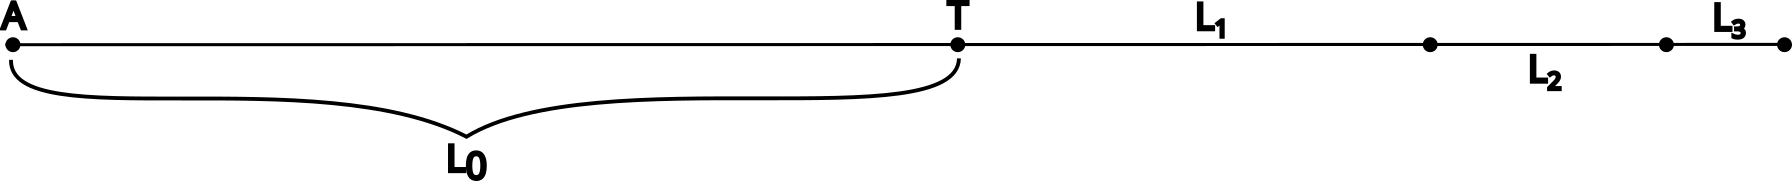
\includegraphics[width=0.7\linewidth]{serie_numeriche/zenone.png}
	\caption{Paradosso di Zenone}
	\label{fig:zenone}
\end{figure}

A Achille, T tartaruga, $v_A>v_T$ 

\begin{align*}
\centering
L_0 & \qquad t_0 = \frac{L_0}{v_A} 
\\
L_1=t_0\cdot v_T & \qquad t_1=\frac{L_1}{v_A} = t_0\frac{v_T}{v_A}
\\
L_2=t_1\cdot v_T & \qquad t_2=\frac{L_2}{v_A} = t_1 \frac{v_T}{v_A} = t_0 \biggl( \frac{v_T}{v_A} \biggr) ^2 
\\
L_3=t_2\cdot v_T & \qquad t_3=\frac{L_3}{v_A} =  t_0 \biggl( \frac{v_T}{v_A} \biggr) ^3
\end{align*}
Quanto tempo impiega Achille a raggiungere la tartaruga?

\newcommand\zenone{\stackrel{\mbox{\tiny{$v_T<v_A$}}}{=}}

\begin{align*}
	T   &= t_0 + t_1 + t_2 + \ldots = t_0 \biggl(1 + \frac{v_T}{v_A} + \biggl(\frac{v_T}{v_A}\biggr)^2 + \ldots + \biggl(\frac{v_T}{v_A}\biggr)^n + \ldots \biggr)	= t_0 \sum_{k=0}^\infty \biggl(\frac{v_T}{v_A}\biggr)^k = \\
	&\zenone t_0 \frac{1}{1-\frac{v_T}{v_A}} = \frac{\frac{L_0}{v_A}}{1-\frac{v_T}{v_A}}
\end{align*}

\subsubsection{Serie geometrica} di ragione r, con $r\in\mathbb{C}$

\begin{equation*}
	\sum_{k=0}^\infty r^k = r^0 + r^1 + r^2 + \ldots
\end{equation*}

\begin{itemize}
	\item $r=1$
	\begin{align*}
		\sum_{k=0}^\infty 1^k
		&= \lim_{n} \sum_{k=0}^n 1^k = \lim_{n} \underbrace{(1 + 1 + \ldots +1)}_\text{n+1 volte} = \\
		&=\lim_{n} (n+1) = +\infty
	\end{align*}
	
	\item $r\neq1$ \qquad Procuriamoci un'espressione della ridotta n-esima, cioè 
	\begin{equation*}
		S_n = \sum_{k=0}^n r^k = 1 + r + r^2 + \ldots + r^n
	\end{equation*}
	
	\begin{gather*}
		\begin{cases*}
			S_{n+1} = \sum_{k=0}^{n+1} r^k = \underbrace{1 + r + r^2 + \ldots + r^n}_\text{$S_n$} + r^{n+1} = S_n + r^{n+1} \\
			S_{n+1} = 1 + \underbrace{r + r^2 +r^3 + \ldots + r^n + r^{n+1}}_\text{raccolgo r a fattore comune} = 1 + r(1 + r + r^2 + \ldots + r^n) = 1 + rS_n
		\end{cases*}  \Rightarrow
		\\
		\Rightarrow S_n + r^{n+1} = 1 + rS_n
	\end{gather*}
	

	
	\begin{equation}
		S_n = \frac{1 - r^{n+1}}{1-r}
	\end{equation}
\end{itemize}

\begin{exbar}
	Per Achille e la Tartaruga $r=\frac{v_T}{v_A}$.
\end{exbar}

\begin{attbar}
	$\lim_{n} S_n = \lim_{n} \frac{1-r^{n+1}}{1-r} \exists$ finito e vale in tal caso $\frac{1}{1-r} \iff |r|<1$
\end{attbar}

\begin{attbar}
	La serie geometrica di ragione $r$, $\sum_{k=0}^\infty r^k$ converge $\iff |r|<1$ e in tal caso la sua somma vale $\frac{1}{1-r}$.
\end{attbar}

\begin{exbar}
	\begin{example} Dimostriamo che $0.\bar{9} = 1$
		\begin{align*}
			0.\bar{9} 
			&= \sum_{k=1}^\infty \frac{9}{10^k} = \lim_{n\rightarrow+\infty} \sum_{k=1}^n \frac{9}{10^k} = 9 \lim_{n\rightarrow+\infty} \sum_{k=1}^n \frac{1}{10^k} = 9 \lim_{n\rightarrow+\infty} \biggl( \sum_{k=0}^n \frac{1}{10^k} - \frac{1}{10^0} \biggr) = \\
			&= 9 \biggl( \sum_{k=0}^\infty \biggl(\frac{1}{10} \biggr)^k - 1 \biggr) = 9 \biggl( \frac{1}{1-\frac{1}{10}} -1 \biggr) = 9 \biggl( \frac{10}{9} -1 \biggr) = \\
			&=1
		\end{align*}	
	\end{example}
\end{exbar}

\subsubsection{Serie telescopiche}
\begin{equation*}
	\sum_{k=0}^\infty [f(k+1) - f(k)] \qquad f:\mathbb{N}\rightarrow\mathbb{C}
\end{equation*}


Studiamo il carattere. Procuriamoci, se possibile, l'espressione di una ridotta n-esima
\begin{align*}
	S_n &= \sum_{k=0}^n [f(k+1)-f(k)] = \\
	&= \overbrace{\cancel{f(1)}-f(0)}^{k=0} + \overbrace{\cancel{f(2)}-\cancel{f(1)}}^{k=1} + \overbrace{\cancel{f(3)}-\cancel{f(2)}}^{k=2} +  \overbrace{\cancel{f(4)}-\cancel{f(3)}}^{k=3} + \ldots + \overbrace{f(n+1)-\cancel{f(n)}}^{k=n} = \\
	&= f(n+1) -f(0)
\end{align*}
\begin{attbar}
	$\lim_{n}S_n = \lim_{n}[f(n+1)-f(0)]$ esiste $\iff$ esiste $\lim_{n} f(n)$.
	
	La serie converge $\iff$ $\lim_{n} f(n)$ esiste finito e in tal caso la somma della serie è 
	\begin{equation*}
			\sum_{k=0}^\infty [f(k+1)-f(k)] = \lim_{n\rightarrow+\infty} f(n)-f(0)
	\end{equation*}

\end{attbar}

\begin{exbar}
	\begin{example} (serie di Mengoli)
		\begin{align*}
			\sum_{k=1}^\infty \frac{1}{k(k+1)} 
			&= \sum_{k=1}^\infty \biggl( \frac{1}{k} -\frac{1}{k+1} \biggr) \\
			&= -\sum_{k=1}^\infty \biggl[\frac{1}{k+1} - \frac{1}{k}\biggr] & \mathrm{dove} \, \frac{1}{k}=f(k) \\
			&= -\lim_{n}[f(n)-f(1)] = f(1) = \\
			&= 1
		\end{align*}
	\end{example}
\end{exbar}

\subsubsection{Formula di Eulero} 

\begin{gather*}
	e^{i\theta} = \cos(\theta) + i \sin(\theta) 
	\\	
	e^{in\theta} = \cos(n\theta) + i\sin(n\theta)
	\\	
	\sum_{n=0}^\infty [\cos(n\theta)+i\sin(n\theta)] = \sum_{n=0}^\infty e^{in\theta} =  \sum_{n=0}^\infty (e^{i\theta})^n
\end{gather*}
Non converge, perché è una serie geometrica di ragione $e^{i\theta}$ e $|e^{i\theta}| = 1$.

Se $\theta = 0, 2\pi$:
\begin{itemize}
	\item $\sum_{n=0}^\infty \cos(n\theta) = \sum_{n=0}^\infty 1 = +\infty$
	\item $\sum_{n=0}^\infty \sin(n\theta) = \sum_{n=0}^\infty 0 = 0$
\end{itemize}

Se $\theta \neq 0, 2\pi$:
\begin{itemize}
	\item $\sum_{k=0}^n \cos(k\theta) = \mathrm{Re} \bigg(\sum_{k=0}^n (e^{i\theta})^k \bigg) = \mathrm{Re} \bigg( \frac{1-e^{i\theta(n+1)}}{1-e^{i\theta}} \bigg)$
	\item $\sum_{k=0}^n \sin(k\theta) = \mathrm{Im} \bigg(\sum_{k=0}^n (e^{i\theta})^k \bigg) = \mathrm{Im} \bigg( \frac{1-e^{i\theta(n+1)}}{1-e^{i\theta}} \bigg)$
\end{itemize}

\begin{align*}
	& \qquad \frac{1-e^{i\theta(n+1)}}{1-e^{i\theta}} \\
	&= \frac{1 - \cos[(n+1)\theta] - i \sin[(n+1)\theta]}{1-\cos\theta - i \sin\theta} \\
	&= \frac{1 - \cos[(n+1)\theta] - i\sin[(n+1)\theta]}{|1-\cos\theta-i\sin\theta|^2} \cdot (1 - \cos\theta + i\sin\theta) \\
	&= \frac{1}{2(1-\cos\theta)} \cdot \{1 - \cos[(n+1)\theta] - i\sin[(n+1)\theta]\} \cdot (1 - \cos\theta + i\sin\theta)= \\
	&= \frac{1}{2(1-\cos\theta)} \cdot \{ 1 - \cos\theta - \cos[(n+1)\theta] + \cos\theta\cos[(n+1)\theta] + \sin\theta\sin[(n+1)\theta] + \\
	& \quad + i[\sin\theta-\cos[(n+1)\theta]\sin\theta - \sin[(n+1)\theta] + \sin[(n+1)\theta] \cos\theta ] \}
\end{align*}

Separiamo parte reale e immaginaria e raccogliamo:
\begin{gather*}
	\sum_{k=0}^n \cos(k\theta) =  \frac{1}{2(1-\cos\theta)} \cdot [(1-\cos\theta)(1-\cos((n+1)\theta)) + \sin\theta\sin((n+1)\theta)]
	\\
	\sum_{k=0}^n \sin(k\theta) =  \frac{1}{2(1-\cos\theta)} \cdot [\sin\theta(1-\cos((n+1)\theta)) - \sin((n+1)\theta)(1-\cos\theta)]
\end{gather*}	
	
	
\subsection{Studio del carattere di una serie}
\begin{theorem}
	\label{th:termine generale}
	$\{a_k \}_{k\in\mathbb{N}} \subseteq \mathbb{C}$ $($oppure $\mathbb{R})$. Se $\sum_{k=0}^\infty a_k$ converge, allora $\lim_{k\rightarrow+\infty} a_k = 0$.
\end{theorem}
Se una serie è convergente il suo termine generale è infinitesimo.

\begin{exbar}
	\begin{example} (serie armonica)
		
		\textbf{Non è vero} che $\lim_{k\rightarrow+\infty} a_k = 0 \Rightarrow \sum_{k=0}^\infty a_k$ converge.
		
		$\sum_{k=1}^\infty \frac{1}{k}$ serie armonica diverge, ma $\lim_{k\rightarrow+\infty}\frac{1}{k} = 0$.
		
		Prendiamo $x$ compresa tra due numeri interi $k$ e $k+1$, con $k\geq 1$.
		\begin{gather*}
			k\leq x \leq k+1
			\\
			\frac{1}{k+1} \leq \colorbox{yellow}{\parbox{1.1cm}{$\frac{1}{x} \leq \frac{1}{k}$}}
			\\
			\int_{k}^{k+1} \frac{1}{x} \mathrm{d}x \leq \int_{k}^{k+1} \frac{1}{k} \mathrm{d}x = \frac{1}{k}
			\\
			\frac{1}{k} \geq \int_{k}^{k+1} \frac{1}{x} \mathrm{d}x = \ln(k+1) -\ln(k)
			\\
			\sum_{k=1}^n \frac{1}{k} \geq \sum_{k=1}^n [\ln(k+1)-\ln(k)] = \ln(n+1)-\ln(1) = \ln(n+1) 
		\end{gather*}
		
		Per il teorema del confronto $\lim_{n}\sum_{k=0}^n \frac{1}{k} \geq \lim_{n} \ln(n+1) = +\infty \Rightarrow \sum_{k=1}^\infty \frac{1}{k} = +\infty$.
	\end{example}
\end{exbar}

\begin{attbar}
	Il \textbf{Teorema \ref{th:termine generale}} si può rileggere: se $\lim_{k\rightarrow+\infty} a_k \neq 0 \Rightarrow \sum_{k=0}^\infty a_k$ non converge.
\end{attbar}

Riprendendo l'esempio del paragrafo precedente vediamo che i termini generale di $\sin(k\theta)$ e $\cos(k\theta)$ non esistono: $\lim_{k\rightarrow+\infty} \cos(k\theta)$ non esiste se $\theta \neq \frac{\pi}{2}, \frac{3\pi}{2}$ e $\lim_{k\rightarrow+\infty} \sin(k\theta)$ non esiste se $\theta\neq 0, 2\pi$.

\begin{dembar}
	\textbf{Dimostrazione} del \textbf{Teorema \ref{th:termine generale}} 
	
	Sappiamo che $\sum_{k=0}^\infty a_k$ converge.
	
	\begin{gather*}
		S_n = \sum_{k=0}^n a_k \qquad S_{n-1} = \sum_{k=0}^{n-1} a_k
		\\
		S_n - S_{n-1} = \sum_{k=0}^n a_k - \sum_{k=0}^{n-1} a_k = a_n + \sum_{k=0}^{n-1} a_k - \sum_{k=0}^{n-1} a_k = a_n
		\\
		\lim_{n} a_n = \lim_{n} (\vertarrowbox{S_n}{$S$} - \vertarrowbox{S_{n-1}}{$S$}) = 0 
	\end{gather*}
	
	$S\in\mathbb{C}$ somma della serie. $\square$
\end{dembar}

\begin{proposition}
	\label{prop:somma convergenti}
	Siano $\sum_{n=0}^\infty a_n$ e $\sum_{n=0}^\infty b_n$ serie convergenti di somma $S_a$ ed $S_b$ rispettivamente. Allora $\sum_{n=0}^\infty (a_n + b_n)$ converge e la sua somma è $S_a+S_b$
\end{proposition}

\begin{dembar}
	\textbf{Dimostrazione} della \textbf{Proposizione \ref{prop:somma convergenti}}
	
	\begin{equation*}
		\sum_{k=0}^n (a_k + b_k) = \vertarrowbox{\sum_{k=0}^\infty a_k}{$S_a$} + \vertarrowbox{\sum_{k=0}^\infty b_k}{$S_b$} \xrightarrow{n\rightarrow+\infty} S_a + S_b \quad \square 
	\end{equation*}
	
\end{dembar}

\begin{proposition}
	\label{prop:prodotto convergente}
	Sia $\sum_{k=0}^\infty a_k$ serie convergente di somma S e sia $c\in\mathbb{C}$. Allora $\sum_{k=0}^\infty (c \cdot a_k)$ converge e la sua somma è $c \cdot S$
\end{proposition}

\begin{dembar}
	\textbf{Dimostrazione} della \textbf{Proposizione \ref{prop:prodotto convergente}}
	\begin{equation*}
		\sum_{k=0}^n (c\cdot a_k) = c\vertarrowbox{\sum_{k=0}^n a_k}{$S$} \xrightarrow{n\rightarrow+\infty} c\cdot S \quad \square
	\end{equation*}

\end{dembar}

\begin{proposition}
	\label{prop:stesso carattere}
	Sia data la serie $\sum_{k=0}^\infty a_k$ e sia $n_0\in\mathbb{N}$, $n_0\geq1$. Allora $\sum_{k=0}^\infty a_k$ e $\sum_{k=n_0}^\infty a_k$ hanno lo stesso carattere.
\end{proposition}

\begin{exbar}
	$\sum_{k=1}^\infty \frac{1}{k}$ e $\sum_{k=10^{10}}^\infty \frac{1}{k}$ hanno lo stesso carattere, quindi $\sum_{k=10^{10}}^\infty \frac{1}{k} = +\infty$.
\end{exbar}

\begin{attbar}
	Il carattere di una serie dipende solo dalla coda della successione dei suoi termini.
\end{attbar}

\begin{dembar}
	\textbf{Dimostrazione} della \textbf{Proposizione \ref{prop:stesso carattere}}
	
	Sia $n_0<n$ e $\sum_{k=0}^n a_k = \sum_{k=0}^{n_0-1} a_k + \sum_{k=n_0}^n a_k$
	
	$\lim_{n} \sum_{k=0}^n a_k$ esiste $\iff \exists \lim_{n\rightarrow+\infty} \sum_{k=n_0}^n a_k$ per la \textbf{Proposizione \ref{prop:somma convergenti}} e in tal caso 
	
	$\lim_{n} \sum_{k=0}^n a_k = \bigg(\lim_{n} \sum_{k=n_0}^n a_k \bigg) + \bigg(\sum_{k=0}^{n_0-1}a_k\bigg). \quad \square$
\end{dembar}

\begin{definition}
	Sia $\{a_n\}_{n\in\mathbb{N}}$ successione in $\mathbb{R}$ o in $\mathbb{C}$. Allora $\{a_n\}_{n\in\mathbb{N}}$ si dice di Cauchy se $\forall \; \varepsilon > 0 \; \exists \; N>0 \mid \forall \; n>N$ e $p\geq0$ \quad $\mid a_{n+p} - a_n \mid < \varepsilon$.
\end{definition}

\begin{theorem} (criterio di Cauchy per le successioni)
	Sia $\{a_n\}_{n\in\mathbb{N}}$ successione in $\mathbb{R}$ o in $\mathbb{C}$. Allora $\{a_n\}_{n\in\mathbb{N}}$ è convergente $\iff$ è di Cauchy
\end{theorem}

\begin{theorem} (criterio di Cauchy per le serie)
	\label{th:Cauchy serie}
	Sia data una serie $\sum_{k=0}^\infty a_k$ in $\mathbb{R}$ o in $\mathbb{C}$. Allora la serie converge $\iff \forall \; \varepsilon > 0 \; \exists \; N>0 \; \mid$ se $n>N$ e $p\geq0$ \quad $\biggl| \sum_{k=n}^{n+p} a_k \biggr| < \varepsilon$.
\end{theorem}

{\noindent Si ricava dal criterio di Cauchy per le successioni osservando che $\sum_{k=n}^{n+p} a_k = S_{n+p} - S_{n-1}$ \par}

\begin{proposition}
	\label{prop:no indeterminata}
	Sia $\sum_{k=0}^\infty a_k$ serie a termini definitivamente non negativi $\mathrm{(} \exists \; N>0 \; | \; a_k\geq 0 \; \forall \; k>N \mathrm{)}$. Allora la serie converge o diverge, non può essere indeterminata. 
\end{proposition}

\begin{dembar}
	\textbf{Dimostrazione} della \textbf{Proposizione \ref{prop:no indeterminata}}
	
	Per semplicità assumiamo $a_k \geq 0 \; \forall \; k\in\mathbb{N}$. Devo far vedere che, se $\{S_n \}_{n\in\mathbb{N}}$ è la successione delle ridotte, questa fa limite finito o infinito.
	\begin{equation*}
		S_{n+1} = \sum_{k=0}^{n+1} a_k = a_{n+1} + \sum_{k=0}^n = \vertarrowbox{a_{n+1}}{$\geq 0$} + S_n \geq S_n
	\end{equation*}
	
	$\{S_n \}_{n\in\mathbb{N}}$ è crescente e quindi fa limite finito o a $+\infty$. \quad $\square$
\end{dembar}

\begin{theorem}
	\label{th:convergenza assoluta}
	Sia data la serie $\sum_{k=0}^\infty a_k$ e si supponga che $\sum_{k=0}^\infty |a_k|$ converga (si dice che $\sum_{k=0}^\infty a_k$ converge assolutamente). Allora anche $\sum_{k=0}^\infty a_k$ converge e in tal caso $\bigg| \sum_{k=0}^\infty a_k \biggr| \leq \sum_{k=0}^\infty |a_k|$.
\end{theorem}

\begin{dembar}
	\textbf{Dimostrazione} del \textbf{Teorema \ref{th:Cauchy serie}}
	
	Siccome $\sum_{k=0}^\infty |a_k|$ converge, $\forall \; \varepsilon>0 \; \exists \; N>0 \; | $ se $n>N$ e $p\geq 0$ \quad $\sum_{k=n}^{n+p} |a_k| < \varepsilon$
	
	$\bigg| \sum_{k=n}^{n+p} a_k \bigg| \distr \sum_{k=n}^{n+p} |a_k| < \varepsilon$ se $n>N$ e $p\geq0 \Rightarrow$ la serie soddisfa la condizione di Cauchy e quindi converge.
	
	In tal caso 
	\begin{align*}
		\bigg| \sum_{k=0}^\infty a_k \bigg|
		& \quad = \bigg|\lim_{n\rightarrow+\infty} \sum_{k=0}^n a_k \bigg| = \lim_{n\rightarrow+\infty} \bigg| \sum_{k=0}^n a_k \bigg| \\
		&\distr \lim_{n\rightarrow+\infty} \sum |a_k| = \sum_{k=0}^\infty |a_k|. \quad \square
	\end{align*}
\end{dembar}

\begin{definition}
	Una serie si dice semplicemente convergente se converge, ma non necessariamente converge la serie dei moduli.
\end{definition}

\begin{attbar}
	Il \textbf{Teorema \ref{th:convergenza assoluta}} non si può invertire. Una serie potrebbe convergere semplicemente, ma non convergere assolutamente.  
\end{attbar}

\begin{exbar}
	$\sum_{k=1}^\infty \frac{(-1)^k}{k}$ converge, ma $\sum_{k=1}^\infty \bigg| \frac{(-1)^k}{k} \bigg| = \sum_{k=1}^\infty \frac{1}{k}$ è divergente.
\end{exbar}

\subsection{Criteri di convergenza di serie a termini non negativi}
\subsubsection{Criterio del confronto}
\begin{theorem} (criterio del confronto) 
	\label{th:criterio del confronto}
	
	$\{a_k \}_{k\in\mathbb{N}}$, $\{b_k \}_{k\in\mathbb{N}}$ successioni a termini definitivamente non negativi tali che $0\leq a_k \leq b_k$ definitivamente per $k\rightarrow+\infty$.
	
	\begin{enumerate}
		\item Se $\sum_{k=0}^\infty b_k$ converge, allora $\sum_{k=0}^\infty a_k$ converge;
		\item Se $\sum_{k=0}^\infty a_k$ diverge, allora $\sum_{k=0}^\infty b_k$ diverge.
	\end{enumerate}
\end{theorem}

\begin{dembar}
	\textbf{Dimostrazione} del \textbf{Teorema \ref{th:criterio del confronto}}
	
	Definiamo $S_n^b = \sum_{k=0}^n b_k, \; S_n^a = \sum_{k=0}^n a_k$ e per semplicità assumiamo che $a_k \leq b_k \; \forall \; k\geq 0$.
	
	$\lim_{n} S_n^b$ e $\lim_{n} S_n^a$ esistono perché le serie sono a termini definitivamente non negativi. 
	
	Se $\sum_{k=0}^\infty b_k$ converge $\Rightarrow \lim_{n} S_n^b = S^b < +\infty$ 
	
	$a_k \leq b_k \; \forall \; k \Rightarrow S_n^a \leq S_n^b \; \forall \; n$
	
	$\lim_{n} S_n^a \leq \lim_{n} S_n^b < +\infty \Rightarrow \lim_{n} S_n^a$ esiste $\Rightarrow \sum_{k=0}^\infty a_k$ converge.
	
	Se $\sum_{k=0}^\infty a_k$ diverge $\Rightarrow \lim_{n} S_n^a = +\infty$ e $S_n^b \geq S_n^a \; \forall \; n$
	
	$\lim_{n} S_n^b = +\infty$ per il teorema del confronto $\Rightarrow \sum_{k=0}^\infty b_k$ diverge. $\square$
\end{dembar}

\begin{exbar}
	\begin{example} 
		\begin{equation*}
			\sum_{k=1}^\infty \frac{1}{2k(2k-1)}
		\end{equation*}
		
		Ridefiniamo $k \rightarrow 2k-1$, perciò $2k -1$ diventa $k$ e $2k$ diventa $k+1$
		
		\begin{equation*}
			a_k =
			\begin{cases}
				\frac{1}{k(k+1)} & \mathrm{se} \, k \, \mathrm{\grave{e}  \, dispari}, k\geq 1 \\
				0				& \mathrm{se} \, k \, \mathrm{\grave{e} \, pari}
			\end{cases}
		\end{equation*}
		
		$0 \leq a_k \leq \mathcircled{\frac{1}{k(k+1)}}^{\color{blue}{\myarrow[180]} b_k} \; \forall k \in \mathbb{N}, \; k\geq 1$
		
		$\sum_{k=1}^\infty \frac{1}{k(k+1)}$ converge $\Rightarrow \sum_{k=1}^\infty \frac{1}{2k(2k-1)}$ converge per il criterio del confronto.
	\end{example}
\end{exbar}

\begin{exbar}
	\begin{example} Studiare la convergenza della serie 
		\begin{align*}
			&\sum_{k=1}^\infty \frac{3^k [k + i\sin(k^k)\cdot\ln(k) ]}{4^k} = \\
			=& \sum_{k=1}^{\infty} \bigg[k\frac{3^k}{4^k} + i \frac{3^k}{4^k} \sin(k^k) \ln(k) \bigg]
		\end{align*}
		
		(\textbf{Per casa:} studiare la convergenza assoluta utilizzando il criterio del confronto)
		
		Dobbiamo studiare separatamente $\sum_{k=1}^{\infty} k\frac{3^k}{4^k}$ e $\sum_{k=1}^{\infty} \frac{3^k}{4^k} \sin(k^k) \ln(k)$.
		
		\begin{itemize}
			\item Partiamo da $\sum_{k=1}^\infty k\frac{3^k}{4^k} \Rightarrow k \bigg(\frac{3}{4} \bigg)^k \leq \alpha^k \; \exists \; \alpha \in \; ]0,1[ \Rightarrow k\leq \bigg(\frac{4}{3} \alpha \bigg)^k$
			
			Se $\frac{4}{3} \alpha > 1$ è vera definitivamente. Poniamo allora sia $\alpha=\frac{5}{6} \Rightarrow k\bigg(\frac{3}{4} \bigg)^k \leq \bigg(\frac{5}{6} \bigg)^k$ definitivamente $\Rightarrow$ la serie converge. 
			
			\item Passiamo a $\sum_{k=1}^\infty \frac{3^k \sin(k^k)\ln(k)}{4^k}$. Studiamo la convergenza assoluta $\sum_{k=1}^\infty \frac{3^k |\sin(k^k)|\ln(k)}{4^k}$. 
			
			Cerchiamo di confrontare il termine generale con il termine generale di una serie convergente:
			$0 \leq \frac{3^k \overbrace{|\sin(k^k)|}^{\leq 1} \ln(k)}{4^k} \leq k \bigg(\frac{3}{4} \bigg)^k$ e $\sum_{k=1}^\infty k \bigg(\frac{3}{4}\bigg)^k$ converge $\Rightarrow \sum_{k=1}^\infty \frac{3^k \sin(k^k)\ln(k)}{4^k}$ converge per i criteri del confronto e di convergenza assoluta.
		\end{itemize}
	\end{example}
\end{exbar}

\begin{theorem} (criterio del confronto asintotico)
	\label{th:confronto asintotico}
	
	$\{a_k \}_{k\in\mathbb{N}} \; \{b_k \}_{k\in\mathbb{N}}$ successioni definitivamente $\geq 0$ tali che $\lim_{k\rightarrow+\infty} \frac{a_k}{b_k} = \ell \; \in \; [0,+\infty]$
	\begin{enumerate}
		\item se $\ell\in\mathbb{R}^{>0} \; (\ell\neq0,+\infty)$, allora $\sum_{k=0}^\infty a_k$ converge $\iff \sum_{k=0}^\infty b_k$ converge;
		\item se $\ell = 0$ e $\sum_{k=0}^\infty b_k$ converge, allora $\sum_{k=0}^\infty a_k$ converge;
		\item se $\ell = +\infty$ e $\sum_{k=0}^\infty a_k$ diverge, allora $\sum_{k=0}^\infty b_k$.
	\end{enumerate}
\end{theorem}

\begin{dembar}
	\textbf{Dimostrazione} del \textbf{Teorema \ref{th:confronto asintotico}}
	\begin{enumerate}
		\item $\ell \; \in ]0,+\infty[$, $\ell = \lim_{k\rightarrow+\infty} \frac{a_k}{b_k}$. Per la definizione di limite $\frac{\ell}{2} \leq \frac{a_k}{b_k} \leq 2\ell$ definitivamente perché l'intervallo $]\frac{\ell}{2}, 2\ell[$ è un intorno di $\ell$
		\begin{itemize}
			\item \textit{Condizione necessaria $(\Leftarrow)$}: $b_k \leq (2\ell) b_k$ definitivamente. 
			
			Se $\sum_{k=0}^\infty b_k$ converge $\Rightarrow \sum_{k=0}^\infty (2\ell) b_k$ converge $\Rightarrow \sum_{k=0}^\infty a_k$ converge per il criterio del confronto;
			
			\item \textit{Condizione sufficiente $(\Rightarrow)$}: $b_k \leq \frac{2}{\ell} a_k$ definitivamente.
			
			Se $\sum_{k=0}^\infty a_k$ converge $\Rightarrow \sum_{k=0}^\infty \frac{2}{\ell} a_k$ converge $\Rightarrow \sum_{k=0}^{\infty} b_k$ converge per il criterio del confronto.
		\end{itemize}
		
		\item $\ell=0=\lim_{k\rightarrow+\infty} \frac{a_k}{b_k} \Rightarrow \frac{a_k}{b_k} \leq 1$ definitivamente. $0 \leq a_k \leq b_k$ definitivamente. 
		
		Se $\sum_{k=0}^\infty b_k$ converge $\Rightarrow \sum_{k=0}^\infty a_k$ converge.
		
		\item $\ell = +\infty = \lim_{k\rightarrow+\infty} \frac{a_k}{b_k} \Rightarrow \frac{a_k}{b_k} \geq 1$ definitivamente $\Rightarrow a_k \geq b_k \geq 0$ definitivamente.
		
		Se $\sum_{k=0}^\infty a_k$ diverge $\Rightarrow \sum_{k=0}^\infty b_k$ diverge per il criterio del confronto. $\square$
	\end{enumerate}
\end{dembar}

\begin{theorem} (criterio di condensazione)
	
	Sia $\{a_k \}_{k\in\mathbb{N}}$ successione a termini positivi e decrescente (basta definitivamente: $0\geq a_{k+1} \geq a_k$ definitivamente). 
	
	Allora $\sum_{k=0}^\infty a_k$ converge $\iff$ converge $\sum_{k=0}^\infty 2^k a_{2^k}$.
\end{theorem}

\begin{exbar}
	\begin{example} (serie armonica generalizzata)
		$$\sum_{k=1}^\infty \frac{1}{k^\alpha} \; , \; \alpha\in\mathbb{R}$$
		
		\begin{itemize}
			\item  Se $\alpha\leq1 \Rightarrow \frac{1}{k^\alpha} \geq \frac{1}{k} \; \forall \; k\geq1$
			
			$\sum_{k=1}^\infty \frac{1}{k}$ diverge $\Rightarrow \sum_{k=1}^\infty \frac{1}{k^\alpha}$ diverge per il criterio del confronto.
			
			\item Se Se $\alpha > 1$ utilizziamo il criterio di condensazione perché la successione 		$\biggl\{\frac{1}{k^\alpha} \biggr\}_{k\in\mathbb{N}}$ è positiva e decrescente 
			
			$\sum_{k=1}^\infty \frac{1}{k^\alpha}$ converge $\iff \sum_{k=1}^\infty 2^k \frac{1}{2^{k\alpha}}$ converge
			
			$\sum_{k=1}^\infty \big(2^{(1-\alpha)} \big)^k$ converge $\iff |2^{1-\alpha}| < 1 \iff \alpha > 1$
		\end{itemize}
	\end{example}
\end{exbar}


\begin{attbar}
	\begin{equation*}
		\sum_{k=1}^\infty \frac{1}{k^\alpha} \ \text{converge}  \ \iff \alpha > 1
	\end{equation*}
\end{attbar}


\begin{exbar} 
	\begin{example}\textbf{importante}
		
		Studiamo il carattere della serie 
		$$\sum_{k=2}^\infty \frac{1}{k^\alpha(\ln k)^\beta} \qquad \alpha, \beta \in \mathbb{R}$$
		
		Analizziamo i seguenti casi:
		
		\begin{enumerate}
			\item $\alpha\leq 1, \; \beta \leq 0$
			\begin{gather*}
				\frac{1}{(\ln k)^\beta} = (\ln k)^{\mathcircled{{-\beta}}^{\color{blue}{\myarrow[190] \geq0}}} \geq 1 \qquad \forall \; k \geq 3
				\\				
				\frac{1}{k^\alpha (\ln k)^\beta} \geq \frac{1}{k^\alpha} \qquad \forall \; k \geq 3
			\end{gather*}

			$\frac{1}{k^\alpha}$ è il termine generale di una serie divergente $\Rightarrow \sum_{k=2}^\infty \frac{1}{k^\alpha(\ln k)^\beta}$ diverge.
			
			\item $\alpha > 1, \; \beta \geq 0$
			\begin{equation*}
				\frac{1}{(\ln k)^\beta} \leq 1 \qquad \forall \; k \geq 3 \Rightarrow \frac{1}{k^\alpha (\ln k)^\beta} \leq \frac{1}{k^\alpha}
			\end{equation*}
			
			$\frac{1}{k^\alpha}$ è il termine generale di una serie convergente $\Rightarrow \sum_{k=2}^\infty \frac{1}{k^\alpha(\ln k)^\beta}$ converge per il teorema del confronto.
			
			\item $\alpha<1, \; \beta>0$
			\begin{equation*}
				\frac{1}{k^\alpha (\ln k)^\beta}
			\end{equation*}
						
			Sia $\varepsilon > 0 \Rightarrow \ln k \leq k^\varepsilon$ definitivamente $\Rightarrow (\ln k)^\beta \leq k^{\varepsilon\beta}$ definitivamente 
			\begin{equation*}
				\frac{1}{(\ln k)^\beta} \geq \frac{1}{k^\alpha k^{\varepsilon\beta}} = \frac{1}{k^{\alpha+\varepsilon\beta}} \ \text{definitivamente}
			\end{equation*}
			
			Scelgo $\varepsilon$ in modo che $\alpha+\varepsilon\beta<1$, quindi $\varepsilon<\frac{1-\alpha}{\beta} \Rightarrow \sum_{k=2}^\infty \frac{1}{k^{\alpha+\varepsilon\beta}}$ diverge $\Rightarrow$ per il criterio del confronto $\sum_{k=2}^\infty \frac{1}{k^\alpha (\ln k)^\beta}$ diverge.
			
			\item $\alpha>1, \; \beta<0$ 
			
			(Se $\beta=0$ la serie diventa $\sum_{k=2}^\infty \frac{1}{k^\alpha}$ che converge)
			\begin{equation*}
				\frac{1}{k^\alpha(\ln k)^\beta} = \frac{(\ln k)}{k^{\alpha}}^{\mathcircled{-\beta}^{\color{blue}{\myarrow[190] >0}}}
			\end{equation*}
			
			Fisso $\varepsilon > 0$, $\ln k \leq k^\varepsilon$ definitivamente $\Rightarrow (\ln k)^{-\beta} \leq k^{-\varepsilon\beta}$ definitivamente
			
			$\frac{1}{k^\alpha (\ln k)^\beta} \leq \frac{k^{-\varepsilon\beta}}{k^\alpha} = \frac{1}{k^{\alpha+\varepsilon\beta}}$ definitivamente
			
			Scelgo $\varepsilon > 0$ in modo che $\alpha+\varepsilon\beta > 1$, quindi $\varepsilon<\frac{1-\alpha}{\beta} \Rightarrow \sum_{k=2}^\infty \frac{1}{k^{\alpha+\varepsilon\beta}}$ converge $\Rightarrow$ per il criterio del confronto $\sum_{k=2}^\infty \frac{1}{k^\alpha (\ln k)^\beta}$ converge.
			
			\item $\alpha=1, \; \beta>0$
			
			$\frac{1}{k^\alpha (\ln k)^\beta} \leq  \frac{1}{k} \qquad \forall \; k \geq 3$, che è il termine generale di una serie divergente, perciò non possiamo usare il teorema del confronto
			
			Utilizziamo il criterio di condensazione: $\biggl\{ \mathcircled{{\frac{1}{k(\ln k)^\beta}}}^{\color{blue}{\myarrow[190] a_k}} \biggr\}_{k\geq2}$ è positiva, decrescente, infinitesima
			
			Studiamo la serie $\sum_{k=2}^\infty 2^k a_{2^k} = \sum_{k=2}^\infty \cancel{2^k} \frac{1}{\cancel{2^k}(\ln 2^k)^\beta} = \sum_{k=2}^\infty \frac{1}{(k \ln 2)^\beta} = \frac{1}{(\ln 2)^\beta} \sum_{k=2}^\infty \frac{1}{k^\beta}$ che converge $\iff \beta > 1$		
		\end{enumerate}
	\end{example}	
\end{exbar}

\begin{attbar}
	\begin{equation*}
		\sum_{k=2}^\infty \frac{1}{k^\alpha (\ln k)^\beta} \ \text{converge} \ \iff \alpha>1 \ \text{oppure} \ \alpha=1 \ \text{e} \ \beta>1.
	\end{equation*}
\end{attbar}


\begin{exbar}
	\begin{example}
		Studiare il carattere della serie 
		\begin{gather}
			\sum_{k=3}^\infty \frac{k}{k^3-k^2+k-e^{-k}}
			\\
			\frac{k}{k^3-k^2+k-e^{-k}} \geq 0 \ \text{definitivamente}
		\end{gather}
		
		Cerchiamo di ricondurci al termine generale della serie studiata in precedenza:
		\begin{gather*}
			\frac{k}{k^3-k^2+k-e^{-k}} \sim \frac{1}{k^\alpha (\ln k)^\beta}
			\\
			-k^2+k-e^{-k}= o(k^3) \ \text{per} \ k\rightarrow+\infty
			\\
			\frac{k}{k^3-k^2+k-e^{-k}} \vertarrowbox{\sim}{\text{limite del rapporto è finito e $\neq0$ }} \frac{k}{k^3} = \frac{1}{k^2}
		\end{gather*}

		$\lim_{k\rightarrow+\infty} \frac{\frac{k}{k^3-k^2+k-e^{-k}}}{\frac{1}{k^2}} = 1 \Rightarrow$ poiché $\sum_{k=3}^\infty \frac{1}{k^2}$ converge, $\sum_{k=3}^\infty \frac{k}{k^3-k^2+k-e^{-k}}$ converge per il criterio del confronto asintotico.
	\end{example}
\end{exbar}


\begin{exbar}
	\begin{example}
		$$\sum_{k=1}^\infty \mathcircled{\frac{1}{k^\alpha} (\sqrt{k^4+1} - k^2)}^{\color{blue}{\myarrow[190] \geq 0 \quad \forall \; k\geq 1}} \qquad \alpha\in\mathbb{R}$$
		
		$\sqrt{k^4+1} - k^2 \geq \sqrt{k^4} - k^2 = 0$. Moltiplichiamo numeratore e denominatore per togliere la radice:
		
		\begin{equation*}
		\frac{1}{k^\alpha} \frac{(\sqrt{k^4+1}-k^2)(\sqrt{k^4+1}+k^2)}{\sqrt{k^4+1}+k^2} = \frac{1}{k^\alpha (\sqrt{k^4+1}+k^2)} \sim \frac{1}{k^\alpha\cdot k^2} = \frac{1}{k^{\alpha+2}}
		\end{equation*}
		
		$\sum_{k=1}^\infty \frac{1}{k^{\alpha+2}}$ converge $\iff \alpha+2>1 \iff a>-1$ per il criterio del confronto asintotico.
	\end{example}
\end{exbar}


\begin{exbar}
	\begin{example}
		Determinare per quale $\alpha>0$ converge la serie 
		\begin{equation*}
			\sum_{k=2}^\infty \bigg[\frac{1}{k(\ln k)} - \sin \frac{1}{k^\alpha(\ln k)} \bigg]
		\end{equation*}
		
		L'espansione in serie di Taylor del seno è: $\sin y = y - \frac{y^3}{3!} + \mathrm{o}(y^3)$ per $y\rightarrow0$
		\begin{align*}
			y &= \frac{1}{k^\alpha(\ln k)} \rightarrow 0 \ \text{per} \ k\rightarrow+\infty
			\\
			\sin \frac{1}{k^\alpha (\ln k)}
			&= \frac{1}{k^\alpha (\ln k)} - \frac{1}{6} \bigg(\frac{1}{k^\alpha (\ln k)} \bigg)^3 + \mathrm{o}\bigg( \bigg(\frac{1}{k^\alpha (\ln k)} \bigg)^3 \bigg) 
			\\
			&= \frac{1}{k^\alpha (\ln k)} - \frac{1}{6} \frac{1}{k^{3\alpha}(\ln k)^3} + \mathrm{o}\bigg(\frac{1}{k^{3\alpha}(\ln k)^3} \bigg) & \mathrm{per} \; k \rightarrow + \infty
		\end{align*}
		\begin{gather*}
		\frac{1}{k (\ln k)} - \sin\frac{1}{k^\alpha(\ln k)} = \frac{1}{k (\ln k)} -\frac{1}{k^\alpha (\ln k)} + \frac{1}{6} \frac{1}{k^{3\alpha}(\ln k)^3} + \mathrm{o}\bigg(\frac{1}{k^{3\alpha}(\ln k)^3} \bigg) \sim
		\\
		\sim \begin{cases}
				-\frac{1}{k^\alpha (\ln k)} & \mathrm{se} \; 0<\alpha<1 
				\\[1em]
				\frac{1}{k^3(\ln k)^3} & \mathrm{se} \; \alpha = 1 
				\\[1em]
				\frac{1}{k (\ln k)} & \mathrm{se} \; \alpha > 1
			\end{cases}
		\end{gather*}
		
		\begin{enumerate}
			\item $\sum_{k=2}^\infty \frac{1}{k^\alpha (\ln k)}$ diverge per $\alpha < 1$;
			\item $\sum_{k=2}^\infty \frac{1}{k^3 (\ln k)^3}$ converge;
			\item $\sum_{k=2}^\infty \frac{1}{k (\ln k)}$ diverge.
		\end{enumerate}
		
		Per il criterio del confronto asintotico
		$\sum_{k=2}^\infty \bigg[\frac{1}{k (\ln k)} - \sin \frac{1}{k^\alpha (\ln k)} \bigg]$ converge $\iff \alpha=1$
	\end{example}
\end{exbar}

\subsubsection{Criterio del rapporto}
\begin{theorem} (criterio del rapporto) \label{th:criterio del rapporto}
	
	$\{a_k\}_{k\in\mathbb{N}}$ successione a termini (definitivamente) positivi.
	\begin{enumerate}
		\item Se $\exists \; r<1$ tale che $\frac{a_{k+1}}{a_k} \leq r$ definitivamente per $k\rightarrow+\infty$, allora $\sum_{k=0}^\infty a_k$ converge;
		\item Se $\frac{a_{k+1}}{a_k} \geq 1$ definitivamente per $k\rightarrow+\infty$, allora $\sum_{k=0}^\infty a_k$ diverge.
	\end{enumerate}
\end{theorem}


\begin{dembar}
	\textbf{Dimostazione} del \textbf{Teorema \ref{th:criterio del rapporto}}
	
	Per semplicità, assumiamo che $a_k > 0 \qquad \forall \; k \in\mathbb{N}$
	
	\begin{enumerate}
		\item  $\exists \; r < 1 \; \bigg| \; \frac{a_{k+1}}{a_k} \leq r \qquad \underbrace{\forall \; k\in\mathbb{N}}_{\text{per semplicità}} $ quindi $\frac{a_k}{a_{k-1}} \leq r \qquad k \geq 1$		
		\begin{equation*}
			a_k \leq r a_{k-1} \; \vertarrowbox{\leq}{$\frac{a_{k-1}}{a_{k-2}} \leq r$} \; r^2 a_{k-2} \; \vertarrowbox{\leq}{$\frac{a_{k-2}}{a_{k-3}} \leq r$} \; r^3 a_{k-3} \leq \ldots \leq r^k a_0 \qquad \Rightarrow \qquad a_k \leq r^k a_0 \qquad \forall \; k\in\mathbb{N}
		\end{equation*}
		
		e $\sum_{k=0}^\infty r^k$ converge perché è una serie geometrica di ragione $r\in ]0,1[ \Rightarrow$ per il criterio del confronto $\sum_{k=0}^\infty r^k$ converge.
		
		\item $\frac{a_{k+1}}{a_k} \geq 1 \qquad \underbrace{\forall \; k\in\mathbb{N}}_{\text{per semplicità}}$ quindi $a_{k+1}\geq a_k \qquad \forall \; k$
		
		$\{a_k \}_{k\in\mathbb{N}}$ è successione crescente a termini strettamente positivi 
		
		$\lim_{k\rightarrow+\infty} a_k > 0 \Rightarrow \sum_{k=0}^\infty a_k$ diverge. $\square$ 	
	\end{enumerate}
\end{dembar}


\begin{theorem} (criterio asintotico del rapporto) \label{th:criterio asintotico rapporto}
	$\{a_k \}_{k\in\mathbb{N}}$ successione a termini definitivamente positivi tale che $\lim_{k\rightarrow+\infty} \frac{a_{k+1}}{a_k} = \ell \in \; [0,+\infty]$
	\begin{enumerate}
		\item Se $\ell < 1$, la serie $\sum_{k=0}^\infty a_k$ converge.
		\item Se  $\ell > 1$, la serie $\sum_{k=0}^\infty a_k$ diverge.
	\end{enumerate}	
\end{theorem}

\begin{attbar}
	Il \textbf{Teorema \ref{th:criterio asintotico rapporto}} non dice nulla se $\ell = 1$
\end{attbar}


\begin{exbar}
	$\sum_{k=1}^\infty \mathcircled{\frac{1}{k}}^{\color{blue}{\myarrow[190] a_k}} \qquad \lim_{k\rightarrow+\infty} \frac{a_{k+1}}{a_k} = 1$ e la serie diverge.
	
	$\sum_{k=1}^\infty \mathcircled{\frac{1}{k^2}}^{\color{blue}{\myarrow[190] a_k}} \qquad \lim_{k\rightarrow+\infty} \frac{a_{k+1}}{a_k} = 1$ e la serie converge.
\end{exbar}


\begin{dembar}
	\textbf{Dimostrazione} del \textbf{Teorema \ref{th:criterio asintotico rapporto}}
	
	\begin{enumerate}
		\item $\lim_{k} \frac{a_{k+1}}{a_k} = \ell < 1$. Fissiamo $r\in \; ]\ell, 1[$ allora definitivamente $ \frac{a_{k+1}}{a_k} \leq r \Rightarrow$ la serie converge per il criterio del rapporto.
		
		\item $\lim_{k} \frac{a_{k+1}}{a_k} = \ell > 1 \Rightarrow \frac{a_{k+1}}{a_k} \geq 1$ definitivamente $\Rightarrow$ la serie diverge per il criterio del rapporto. $\square$ 
	\end{enumerate}
\end{dembar}


\begin{exbar}
	\begin{example}
		Studiamo il carattere della serie 
		\begin{equation*}
			\sum_{n=0}^{\infty} \mathcircled{\frac{(2n)!}{n! \ (2n+1)!}}^{\color{blue}{\myarrow[190] a_n}}
		\end{equation*}
		\begin{align*}
			\lim_{n \rightarrow +\infty} \frac{a_{n+1}}{a_n} 
			&= \lim_{n \rightarrow +\infty} \frac{(2n+1)!}{(n+1)! \ (2n+3)^{n+1}} \cdot \frac{n! \ (2n+1)^n}{(2n)!} \\
			&= \inflim \frac{(2n+2) \ (2n+1) \ \cancel{(2n)!}} {(n+1) \ \cancel{n!} \ (2n+3)^{n+1} } \cdot \frac{\cancel{n!} \ (2n+1)^{n}}{\cancel{(2n)!}} \\
			&=\inflim \frac{(2n+2) \ (2n+1)} {(n+1) \ (2n+3)} \cdot \frac{(2n+1)^n} {(2n+3)^n}=\\
			&=\lim_{n \rightarrow +\infty} \frac{(2n+2) \ (2n+1)}{(n+1) \ (2n+3)} \left(1- \frac{2} {2n+3} \right)^n \\
			&= \frac{4}{2} \ e^{-1}=\frac{2}{e}<1
		\end{align*} 
		$\Rightarrow$ la serie converge per il criterio asintotico del rapporto.	
	\end{example}
\end{exbar}


\begin{exbar}
	\begin{example}
		Studiare il carattere della serie 
		\begin{equation*}
			\sum_{n=1}^{\infty} \mathcircled{ 5^n \ \frac{\left( n! \right)^2}{(2n)!} }^{\color{blue}{\myarrow[190] a_n}}
		\end{equation*}
		\begin{align*}
			\inflim \frac{a_{n+1}}{a_n} 
			&= \inflim 5^{\cancel{n}+1} \frac{((n+1)!)^2}{(2n+2)!} \cdot \frac{(2n)!}{\cancel{5^n} \ (n!)^2}=\\
			&= \inflim 5\frac{(n+1)^2 \ \cancel{(n!)^2}} {(2n+2) \ (2n+1) \ \cancel{(2n)!} } \cdot \frac{\cancel{(2n)!}} {\cancel{(n!)^2}}=\\
			&= \inflim 5\frac{(n+1)^2} {(2n+2) \ (2n+1)} = \frac{5}{4} > 1
		\end{align*}
		
		$\Rightarrow$ la serie diverge per il criterio asintotico del rapporto.	
	\end{example}
\end{exbar}


\begin{exbar}
	\begin{example} \textbf{importante}
		
		\begin{equation*}
			\sum_{k=0}^\infty \frac{z^k}{k!} \qquad z \in  \mathbb{C} 
		\end{equation*}
		
		Studiamo la convergenza assoluta 
		\begin{equation*}
			\sum_{k=0}^\infty \mathcircled{ \frac{|z|^k}{k!} }^{\color{blue}{\myarrow[190] a_k}}
		\end{equation*}
		\begin{align*}
		\lim_{k \rightarrow +\infty} \frac{a_{k+1}}{a_k}
		&= \lim_{k \rightarrow +\infty} \frac{|z|^{k+1}}{(k+1)!} \cdot \frac{k!}{z^k}=\\
		&= \lim_{k \rightarrow +\infty} \frac{|z|}{k+1} = 0 \qquad \forall z \in \mathbb{C}
		\end{align*}
		
		la serie converge assolutamente, e quindi semplicemente, $\forall \ z \in \mathbb{C}$.
		
		Se $x \in \mathbb{R}$ , si dimostra che 
		\begin{equation*} 
			\sum_{k=0}^{\infty} \frac{x^k}{k!}=e^x 
		\end{equation*}.
		
		Se $z \in \mathbb{C}$ , si definisce la serie esponenziale
		\begin{equation*}
			e^z= \mathcircled{\sum_{k=0}^{\infty} \frac{z^k}{k!}} ^ {\color{blue}{\text{ Serie esponenziale}}}
		\end{equation*}
	\end{example}
\end{exbar}

\subsubsection{Criterio della radice}
\begin{theorem} (criterio della radice) 
	\label{th:criterio della radice}
	
	Sia $\{ a_k\}_{k \ \in \mathbb{N}}$ una successione a termini definitivamente non negativi
	\begin{enumerate}
		\item Se $\exists \ r< 1$ tale che $\sqrt[k]{a_k} \leq r$ definitivamente, allora $\sum_{k=0}^{\infty} a_k$ converge.
		\item Se $\sqrt[k]{a_k} \geq 1$ definitivamente, allora $\sum_{k=0}^{\infty} a_k$ diverge.
	\end{enumerate}
\end{theorem}


\begin{dembar}
	\textbf{Dimostrazione} del \textbf{Teorema} \ref{th:criterio della radice} 
	
	\begin{enumerate}
		\item $\sqrt[k]{a_k}\leq r$ definitivamente $\Rightarrow 0 \leq a_k \leq r^k$ definitivamente e dunque $\sum_{k=0}^{\infty} r^k$ converge (perché $r \in [0,1[$) $\Rightarrow \sum_{k=0}^{\infty} a_k$ converge per il criterio del confronto.
		
		\item $\sqrt[k]{a_k} \geq 1$ definitivamente $\Rightarrow a_k \geq 1$ definitivamente $\Rightarrow \lim_{k \rightarrow + \infty} a_k \geq 1$, se esiste $\Rightarrow \sum_{k=0}^{\infty} a_k$ diverge. $\square$ 
	\end{enumerate}
\end{dembar}


\begin{theorem} (criterio asintotico della radice) 
	
	\label{th:criterio asintotico della radice}
	$\{a_k\}_{k \in \mathbb{N}}$ successione a termini definitivamente non negativi tale che $\lim_{k \rightarrow +\infty} \sqrt[k]{a_k} = l \in [0,+\infty[$.
	\begin{enumerate}
		\item Se $l<1$ la serie $ \sum_{k=0}^{\infty} a_k$ converge.
		\item Se $l> 1$ la serie $\sum_{k=0}^{\infty} a_k$ diverge.
	\end{enumerate}
\end{theorem}


\begin{dembar}
	\textbf{Dimostrazione} del \textbf{Teorema} \ref{th:criterio asintotico della radice} 
	\begin{enumerate}
		\item Per $\lim_{k \rightarrow +\infty} \sqrt[k]{a_k} = l < 1$ fisso $r\in \,\,]l,1[\,\, \Rightarrow \sqrt[k]{a_k} =r$  definitivamente $\Rightarrow \sum_{k=0}^{\infty} a_k$ converge per il criterio della radice.
		\item Per $\lim_{k \rightarrow +\infty} \sqrt[k]{a_k} = l > 1 \Rightarrow \sqrt[k]{a_k}\geq 1$ definitivamente  $\Rightarrow \sum_{k=0}^{\infty} a_k$ diverge per il criterio della radice. $\square$
	\end{enumerate}
\end{dembar}


\begin{attbar}
	\textbf{N.B.} Se $\{a_k\}_{k \in \mathbb{N}}$ è a termini definitivamente positivi e  $\lim_{k \rightarrow +\infty} \frac{a_{k+1}}{a_k} = \ell$, allora \\ $\lim_{k \rightarrow +\infty} \sqrt[k]{a_k} = \ell$.
\end{attbar}


\begin{exbar}
	\begin{example}
		Studiamo il carattere della serie
		\begin{equation*}
			\sum_{n=1}^{\infty} \mathcircled{(n+1)^2 \ e^{-(n+1)}}^ {\color{blue}{\myarrow[190] a_n}}
		\end{equation*}
		\begin{align*}
			\inflim \sqrt[n]{a_n} 
			&= \inflim \sqrt[n]{(n+1)^2 e^{-(n+1)}} 
			\\
			&= \inflim \vertarrowbox{\mathcircled{\sqrt[n]{(n+1)^2}}} {\color{blue}{$(n+1)^{\frac{2}{n}}$}} \ 
			\vertarrowbox{\mathcircled{e^{-\frac{n+1}{n}} }}{\color{blue}{$\frac{1}{e}$}}
		\end{align*}
		
		Abbiamo che $(n+1)^{\frac{2}{n}} = e^{\frac{2}{n}} \ \ln(n+1) \rightarrow 1$, perciò
		\begin{equation*}
			\sum_{n=1}^{\infty} = \frac{1}{e} < 1
		\end{equation*} 
		
		$\Rightarrow$ la serie converge per il criterio asintotico della radice.
	\end{example}
\end{exbar}


\begin{exbar}
	\begin{example} \textbf{importante}
		
		Studiamo il carattere della serie
		\begin{equation*}
			\sum_{k=1}^{\infty} k^\alpha \ r^k \qquad r \ \in \mathbb{R}, \ \alpha \ \in \mathbb{R}.
		\end{equation*}
		
		Studiamo la convergenza assoluta
		\begin{gather*}
			\sum_{k=1}^{\infty} |k^\alpha \ r^k| 
			= \sum_{k=1}^{\infty} \mathcircled{k^\alpha \ |r|^k}_{\color{blue}{\myarrow[180] a_k}} 
			\\
			\lim_{k \rightarrow +\infty} \sqrt[k]{a_k} 
			= \lim_{k \rightarrow +\infty} |r| \ k^{\frac{\alpha}{k}}= |r|
		\end{gather*}
		
		Se $|r|< 1$ la serie converge assolutamente e quindi semplicemente.
		
		Se $|r|> 1$, il termine generale della serie non è infinitesimo
		\begin{equation*}
			\lim_{k \rightarrow +\infty} k^\alpha \ |r|^k = +\infty
		\end{equation*} 
		
		e quindi la serie non converge.
		
		Prendiamo dunque $|r|=1$
		\begin{itemize}
			\item Se $r=1$:
			\begin{equation*}
				\sum_{k=1}^{\infty} k^\alpha=\sum_{k=1}^{\infty} \frac{1}{k^{-\alpha}}
			\end{equation*}
			che converge $\iff -\alpha <1 \iff \alpha < -1$
			
			\item Se $r=-1$:
			\begin{equation*}
				\sum_{k=1}^{\infty} \left| k^\alpha(-1)^k \right| =\sum_{k=1}^{\infty} k^\alpha
			\end{equation*} 
			che converge assolutamente $\iff \alpha<-1$.

			Studiamo la convergenza semplice:
			\begin{equation*}
				\sum_{k=1}^{\infty} \frac{(-1)^k}{k^{-\alpha}} \ \text{converge} \vertarrowbox{\iff}{lo vedremo dopo} -\alpha > 0  \iff \alpha <0
			\end{equation*}
			Se $\alpha \geq 0$, $ \lim_{k \rightarrow +\infty} \left| k^\alpha(-1)^k \right| \neq 0 \Rightarrow $ la serie non converge. 
		\end{itemize}
	\end{example}
\end{exbar}


\begin{attbar}
	$\sum_{k=1}^{\infty} k^\alpha \ r^k$ converge assolutamente $\iff |r|<1$ o $r=1$ e $\alpha<-1$ o $r=-1$ e $ \alpha <-1$.
	
	Converge semplicemente, ma non assolutamente $\iff r=-1$ e $ -1<\alpha<0$.
\end{attbar}


\begin{exbar}
	\begin{example} (Serie Logaritmica)
		\begin{equation*}
			\sum_{k=1}^{\infty} (-1)^{k+1} \ \frac{z^k}{k} \qquad z \ \in \mathbb{C}
		\end{equation*}
		Studiamo la convergenza assoluta
		\begin{gather*}
			\sum_{k=1}^{\infty} \left| (-1)^{k+1} \ \frac{z^k}{k} \right| = \sum_{k=1}^{\infty} \mathcircled{\frac{|z|^k}{k}}^{\color{blue}{\myarrow[190] a_k}}
			\\
			\lim_{k \rightarrow +\infty} \sqrt[k]{a_k} = \lim_{k \rightarrow +\infty} \frac{|z|}{\sqrt[k]{k}}= |z|
		\end{gather*}
		
		Se $|z|< 1$, la serie converge assolutamente e quindi semplicemente.
		
		Se $ |z|> 1$, il termine generale della serie non è infinitesimo, e quindi la serie non converge.
		
		Possiamo anche ricondurci al caso precedente:
		\begin{align*}
			\sum_{k=1}^{\infty} (-1)^{k+1} \ \frac{z^k}{k} 
			& = - \sum_{k=1}^{\infty} \frac{(-1)^k z^k }{k}= - \sum_{k=1}^{\infty} \frac{(-z)^k}{k}=
			\\
			& = - \sum_{k=1}^{\infty} \frac{r^k}{k} = - \sum_{k=1}^{\infty} k^\alpha r^k & \text{con} \ \alpha =-1
		\end{align*}
		
		Per $z=x \in \mathbb{R}$ se $ |x|<1$ la serie converge assolutamente mentre se $|x|>1$ allora la serie non converge.
		Se $ |x|=1$ allora 
		\begin{itemize}
			\item $x=-1$: 
			\begin{equation*}
				\sum_{k=1}^{\infty} (-1)^{k+1} \ \frac{(-1)^k}{k} = -\sum_{k=1}^{\infty} \frac{1}{k}
			\end{equation*}  
			che diverge;
			
			\item $x=1$:
			\begin{equation*}
				\Rightarrow \sum_{k=1}^{\infty} (-1)^{k+1} \frac{1}{k} = -\sum_{k=1}^{\infty} \frac{(-1)^k}{k}
			\end{equation*} che converge.
		\end{itemize}
		
		Se $-1<x\leq 1$, allora 
		\begin{equation*}
			\sum_{k=1}^{\infty} (-1 )^{k+1} \ \frac{x^e}{k}= \ln(1+x)
		\end{equation*}
	\end{example}
\end{exbar}


\subsection{Criteri di convergenza di serie a termini di segno qualsiasi}
\subsubsection{Criterio di Dirichelet}
\begin{theorem} (criterio di Dirichelet)
	
	Sia $\{a_k\}_{k \in \mathbb{N}}$ successione a termini non negativi, decrescente, infinitesima (basta definitivamente: $\lim_{k \rightarrow +\infty} a_k=0$ e $0\leq a_{k+1} \leq a_k$ definitivamente per $k \rightarrow +\infty$) e sia $\{b_k\}_{k \in \mathbb{N}} \subseteq \mathbb{C}$ un'altra successione tale che $\exists \ C>0$ per cui vale
	\begin{equation*}
		\left| \sum_{k=0}^{n} b_k \right| \leq C \qquad \forall n \in \mathbb{N}
	\end{equation*}
	(la successione delle ridotte della serie $\sum_{k=0}^{\infty} b_k$ è limitata)
	
	Allora la serie $\sum_{k=0}^{\infty} a_k \ b_k$ converge.
\end{theorem}


\begin{exbar}
	\begin{example}
		\begin{equation*}
			\sum_{k=1}^{\infty} \frac{e^{ik\theta}}{k}, \qquad \theta \in [0, 2\pi[
		\end{equation*}
		
		Per $\theta = 0$ avremo $\sum_{k=1}^{\infty} \frac{1}{k}$ che diverge.
		
		Per $\theta \in \ ]0,2\pi[$ avremo $a_k=\frac{1}{k}$ (che è successione positiva, decrescente e infinitesima) e $b_k= e^{ik\theta}$, dunque:
		\begin{equation*}
			\sum_{k=1}^{n} b_k = \sum_{k=1}^{n} e^{ik\theta} = \frac{1-e^{i(n+1)\theta}}{1-e^{i\theta}}-1 
		\end{equation*} 

		$\sum_{k=1}^{n} e^{ek\theta}$ è la ridotta n-esima di una serie geometrica di ragione $e^{i\theta}$ a cui manca il termine con $k=0$
		\begin{align*}
			\left| \sum_{k=1}^{\infty} b_k \right| 
			&= \left| \frac{e^{i\theta} - e^{i(n+1)\theta}} {1 - e^{i\theta}} \right| 
			\\
			\distr & \frac{\mathcircled{|e^{i \theta}|}^{\ \textcolor{blue}{=1}} + \mathcircled{|e^{i (n+1) \theta}|}^{\ \textcolor{blue}{=1}}} {|1 - e^{i \theta}|}  \leq \frac{2} {|1 - e^{i \theta}|} = 0 \Rightarrow 
		\end{align*}
		
		$\sum_{k=1}^{\infty} \frac{e^{ik\theta}}{k}$ converge $\forall \ \theta \in \ ]0,2\pi[$ per il criterio di Dirichlet
		\begin{equation*}
			\sum_{k=1}^{\infty} \frac{e^{ik\theta}} {k} = \sum_{k=1}^{\infty} \left[ \frac{\cos{k\theta}} {k} + i \ \frac{\sin{k\theta}} {k} \right]
		\end{equation*}
		
		Se $\theta \in \ ]0,2\pi[$ convergono entrambe le serie  $\sum_{k=1}^{\infty} \frac{cos(k\theta)}{k}$ e $ \sum_{k=1}^{\infty} \frac{sin(k\theta)}{k}$ perché
		\begin{gather*}
			\frac{cos(k\theta)}{k}=\Re \left( \frac{e^{ik\theta}} {k} \right) \\ \frac{sin(k\theta)}{k}=\Im \left( \frac{e^{ik\theta}} {k} \right)
		\end{gather*}	
	\end{example}
\end{exbar}


\subsubsection{Criterio di Leibinitz}
\begin{theorem} (criterio di Leibinitz)
	\label{th:criterio di Leibinitz}
	
	Sia $\{a_k\}_{k\in \mathbb{N}}$ successione a termini non negativi, decrescente, infinitesima. Allora
	\begin{equation*}
		\sum_{k=0}^{\infty} (-1)^k \ a_k 
	\end{equation*}
	converge e, detta $S$ la sua somma, si ha
	\begin{align*}
		\left| \sum_{k=0}^{\infty} (-1)^k \ a_k - S \right| \leq a_{k+1} & \qquad \text{ con } S = \lim_{n \rightarrow +\infty} \sum_{k=0}^{n} (-1)^k \ a_k
	\end{align*}
\end{theorem}


\begin{exbar}
	\begin{example}
		\begin{equation*}
			\sin{1} = \sum_{k=0}^{\infty} (-1)^k \ \frac{1^{2k+1}} {(2k+1)!} = \sum_{k=0}^{\infty} (-1)^k \ \frac{1}{(2k+1)!}
		\end{equation*}
		
		La successione $\left\{ \frac{1}{(2k+1)!} \right\}$ è positiva, decrescente, infinitesima. Posso dunque applicare il criterio di Leibniz.
		\begin{equation*}
			\left| \sum_{k=0}^{\infty} \frac{(-1)^k} {(2k+1)!} - \sin(1) \right| \leq \frac{1}{(2k+1)!} \bigg|_{k=n+1}= \frac{1}{(2n+3)!}
		\end{equation*}
		
		Se voglio una stima di $\sin(1)$ con $10$ cifre decimali esatte devo scegliere $n$ in modo che 
		\begin{equation*}
			\frac{1}{(2n+3)!}<10^{-10} \Rightarrow (2n+3)! > 10^{10}
		\end{equation*}
		
		e otteniamo $n=6$.
		
		\begin{equation*}
			\sum_{k=0}^{6} \frac{(-1)^k}{(2k+1)!}= 1-\frac{1}{3!} +\frac{1}{5!}-\frac{1}{7!} +\frac{1}{9!}-\frac{1}{11!} +\frac{1}{13!}
		\end{equation*}
		
		dà una stima di $\sin(1)$ con $10$ cifre decimali esatte.
		
		\textbf{Esercizio}: Dimostrare il criterio di convergenza utilizzando il criterio di Dirichlet con $b_k=(-1)^k$
	\end{example}
\end{exbar}


\begin{dembar}
	\textbf{Dimostrazione} del \textbf{Teorema \ref{th:criterio di Leibinitz}}
	
	\begin{enumerate}
		\item $\{S_{2n}\}_{n \in \mathbb{N}}$, successione delle ridotte di indice pari, è decrescente, ovvero 
		\begin{equation*}
			S_{2n+2}\leq S_{2n} \qquad \forall \ n
		\end{equation*}
		
		perché la successione $\{a_k\}_{k \in \mathbb{N} }$ è decrescente.
		\begin{align*}
			S_{2n+2} 
			&= \sum_{k=0}^{2n+2} (-1)^k \ a_k= \sum_{k=0}^{2n} (-1)^k \ a_k + (-1)^{2n+1} \ a_{2n+1} + (-1)^{2n+2} \ a_{2n+2} =
			\\
			&= \vertarrowbox {\mathcircled {\sum_{k=0}^{2n} (-1)^k \ a_k} } {\color{blue}{$S_{2n}$}} - \underbrace {a_{2n+1} + a_{2n+2}}_ {\color{blue}{\text{$\leq 0$, perché $\{a_k\}_{k\in\mathrm{N}}$ è decrescente}}} \leq S_{2n}.
		\end{align*}
		
		\item $\{S_{2n+1}\}_{n \in \mathbb{N}}$, successione delle ridotte di indice dispari, è crescente, ovvero 
		\begin{equation*}
			S_{2n+3} \geq S_{2n+1} \qquad \forall \ n \in \mathbb{N}
		\end{equation*} 
		
		perché la successione $\{a_k\}_{k \in \mathbb{N}}$ è decrescente
		\begin{align*}
			S_{2n+3} 
			&= \sum_{k=0}^{2n+3} (-1)^k \ a_k = \mathcircled{\sum_{k=0}^{2n+1} (-1)^k \ a_k}^{\color{blue}{\myarrow[190] S_{n+1}}} + (-1)^{2n+2} \ a_{2n+2} +  (-1)^{2n+3} \ a_{2n+3}=
			\\
			&= S_{2n+1} + \underbrace{a_{2n+2} - a_{2n+3}}_{\color{blue} {\text{$\geq 0$ perché $\{a_k\}_{k\in\mathbb{N}}$ è decrescente}}} \geq S_{2n+1}.
		\end{align*}
		
		\item $S_{2n} = S_{2n-1} + (-1)^{2n} \ a_{2n} = S_{2n-1} + \mathcircled{a_{2n}}^{\color{blue}{\ \geq 0}} \geq S_{2n-1} \geq S_1$
		%LASCIA COSÌ, CON EQUATION DÀ UN BRUTTO SPAZIO TRA IL NUMERO DELL'ITEM E L'EQUAZIONE
		
		$\{S_{2n}\}$ è una successione decrescente inferiormente limitata $\Rightarrow $ ha limite finito.
		\begin{equation*}
			S_{2n+1}=S_{2n} + (-1)^{2n+1} \ a_{2n+1} = S_{2n} - a_{2n+1} \leq S_{2n} \leq S_0
		\end{equation*}
		
		$\{S_{2n+1}\}_{n \in \mathbb{N}}$ è crescente e superiormente limitata $\Rightarrow $ ha limite finito.
		
		\item $\inflim S_{2n} = S^0 \in \mathbb{R}, \; \inflim S_{2n+1}=S^1 \in \mathbb{R} \Rightarrow S^0 = S^1 = S$, somma della serie
		\begin{gather*}
			\left| S_{2n+1} - S_{2n} \right| = \left| a_{2n+1} \right| \rightarrow 0
			\\
			\left| S^0 - S^1 \right| \leq \underbrace{\left| S^0 - S_{2n} \right|}_{\color{blue}{=0 \text{ per } n \rightarrow + \infty}} + \underbrace{\left| S_{2n} - S_{2n+1} \right|}_{\color{blue}{=0 \text{ per } n \rightarrow + \infty}} + \underbrace{\left| S_{2n+1} - S^1 \right|}_{\color{blue}{=0 \text{ per } n \rightarrow + \infty}}
			\\
			S^0 = S^1 = S \in \mathbb{R} \; \Rightarrow \text{la serie converge.}
		\end{gather*}
		
		\item $S_{2n+1} \leq S \leq S_{2n+2}  \quad \forall \ n$ perché la prima è crescente e la seconda è decrescente.
		\begin{align*}
			0\leq S - S_{2n+1} \leq S_{2n+2} - S_{2n+1} 
			&= \sum_{k=0}^{2n+2} (-1)^k \ a_k - \sum_{k=0}^{2n+1} (-1)^k \ a_k = \\ 
			&=\uppercomment{a_{2n+2}}{\text{primo termine}}{\text{escluso da } S_{2n+1}}
		\end{align*}
		\begin{gather*}
			0 \leq S_{2n} - S \leq S_{2n} - S_{2n+1} = \uppercomment{a_{2n+1}}{\text{primo termine}}{\text{escluso da } S_{2n}} 
			\\
			\Rightarrow \left| S_n - S \right| \leq \uppercomment{a_{n+1}}{\text{primo termine}}{\text{escluso da } S_{n}}. \qquad \square
		\end{gather*}
	\end{enumerate}
\end{dembar}


\begin{exbar}
	\begin{example}
		\begin{equation*}
			\sum_{k=1}^{\infty} \frac{(-1)^k} {k^\alpha}, \qquad 0 < \alpha \leq 1
		\end{equation*}
		
		non converge assolutamente, ma $\left\{ \frac{1} {k^\alpha} \right\}_{k \in \mathbb{N}}$ è positiva, decrescente, infinitesima, e quindi la serie converge semplicemente per il criterio di Leibniz.
	\end{example}
\end{exbar}


\begin{exbar}
	\begin{example}
			Studiare il carattere della serie
		\begin{equation*}
			\sum_{n=1}^{\infty} \frac{(-1)^n}{n-\ln(n)}
		\end{equation*}
		
		Studiamo la convergenza assoluta
		\begin{equation*}
			\sum_{n=1}^{\infty} \left| \frac{(-1)^n} {n - \ln(n)} \right| = \sum_{n=1}^{\infty} \frac{1} {n - \ln(n)}
		\end{equation*}
		
		Siccome $\frac{1} {n - \ln(n)} \geq \frac{1}{n} \Rightarrow$ la serie diverge.
		
		Studiamo la convergenza semplice:
		\begin{equation*}
			\sum_{n=1}^{\infty} \frac{(-1)^n} {n - \ln(n)}, \quad a_n = \frac{1} {n - \ln(n)}
		\end{equation*}
		
		e speriamo che $\{a_n\}_{n\in\mathbb{N}}$ sia positiva (Vero!), decrescente (Da dimostrare, almeno definitivamente) , infinitesima (Vero!).
		
		Ci chiediamo allora se $a_{n+1}\leq a_{n}$:
		\begin{gather*}
			\frac{1} {n+1 - \ln(n+1)} \leq \frac{1} {n - \ln(n)} 
			\\
			\cancel{n} - \ln(n) \leq \cancel{n} + 1 - \ln(n+1) 
			\\
			\ln \left( \frac{n+1} {n} \right) \leq 1
			\\
			\ln \left( 1 + \frac{1}{n} \right) \leq 1
		\end{gather*} 
		
		Sappiamo che $1 - \frac{1}{n} \leq 2 < e$ perciò
		\begin{equation*}
			\ln \left( 1 + \frac{1} {n} \right) < \ln(e) = 1
		\end{equation*} 
		
		$\Rightarrow$ la serie converge per il criterio di Leibniz.
	\end{example}
\end{exbar}
		
\begin{exbar}
\begin{example}
	
	Studiare il carattere della serie 
	\begin{equation*}
		\sum_{n=1}^{\infty} (-1)^n \ \frac{n+1}{\sqrt{n^4 + 2} - \ln(n)}
	\end{equation*}
	Studiamo la convergenza assoluta
	\begin{gather*}
		\sum_{n=1}^{\infty} \left| (-1)^n \ \frac{n+1}{\sqrt{n^4 + 2} - \ln(n)} \right| = \sum_{n=1}^{\infty} \frac{n+1}{\sqrt{n^4 + 2} - \ln(n)}
		\\
		\frac{n+1}{\sqrt{n^4 + 2} - \ln(n)} \sim  \frac{n}{n^2} = \frac{1}{n}
	\end{gather*}
	
	$\Rightarrow$ la serie diverge assolutamente per il criterio asintotico del confronto.
	
	Studiamo ora la convergenza semplice
	\begin{equation*}
		\sum_{n=1}^{\infty} (-1)^n \ \frac{n+1}{\sqrt{n^4 + 2} - \ln(n)}
	\end{equation*}
	
	La successione $\left\{ \frac{n+1} {\sqrt{n^4 + 2} - \ln(n)} \right\} _ {n \geq 1}$ è positiva (Vero!), decrescente (Da dimostrare, almeno definitivamente), infinitesima (Vero!)
	
	Devo far vedere che, almeno definitivamente, 
	\begin{gather*}
		\frac{n + 2} {\sqrt{ (n + 1)^4 + 2} - \ln(n + 1)} \leq \frac{n + 1} {\sqrt{n^4 + 2} - \ln(n)}
		\\
		(n + 2) \left( \sqrt{n^4 + 2} -\ln(n) \right) \leq (n + 1) \left( \sqrt{(n + 1)^4 + 2} - \ln(n+1) \right)
 		\\
		f(x) = \frac{x + 1} {\sqrt{x^4 + 2} - \ln(x)} , \qquad x > 0
	\end{gather*}
	
	Se dimostro che $f'(x)<0$ definitivamente per $x \rightarrow +\infty \Rightarrow f$ è decrescente in un intorno di $+\infty \Rightarrow f(n+1) \leq f(n)$ definitivamente. Avremo dunque
	\begin{gather*}
		f(n) = \frac{n + 1} {\sqrt{n^4 + 2} - \ln(n)}
		\\
		f(n+1) = \frac{n + 2} {\sqrt{(n + 1)^4 + 2} - \ln(n+1)}
	\end{gather*}
	
	Calcoliamo la derivata $f'(x)$:
	\begin{align*}
		f'(x)
		&= \frac{\sqrt{x^4 + 2} - \ln(x) - (x + 1) \left[ \frac{4 x^3 } {2 \sqrt{x^4 + 2}} - \frac{1}{x} \right]} {\left( 
			\sqrt{x^4 + 2} - \ln(x) \right)^2} = 
		\\
		&= \frac{x (x^4 + 2) - x \sqrt{x^4 + 2} \ \ln(x) - (x + 1) \left[2x ^ 4 - \sqrt{x^4 + 2} \right] } {x \sqrt{x^4 + 2} \left( \sqrt{x^4 + 2} - \ln(x) \right)^2}
	\end{align*}
	\begin{align*}
		f'(x)<0 
		& \iff x (x^4 + 2) - x \sqrt{x^4 + 2} \ \ln(x) - 2x^4 (x + 1) - (x + 1) \sqrt{x^4 + 2}  < 0
		\\
		&\iff -x^5 - 2x^4 + 2x - x\sqrt{x^4+2} \ln(x) + (x + 1) \sqrt{x^4 + 2} < 0
	\end{align*}
	
		$f'(x) < 0$ definitivamente per $x \rightarrow +\infty$
	\begin{equation*}
		 \iff -x^5 - 2x^4 + 2x - x \sqrt{x^4 + 2} \ \ln(x) + (x+1) \sqrt{x^4 + 2} < 0
	\end{equation*} 
	
	definitivamente per $x\rightarrow +\infty$ cioè
	\begin{align*}
		-x^5 - 2x^4 + 2x \underbrace{- x\sqrt{x^4 + 2} \ln(x)}_{\color{blue}{\sim -x^3 \ln(x)}} \underbrace{+ (x + 1) \sqrt{x^4 + 2}}_{\color{blue}{\sim x^3}} &< 0 
		\\
		-x^5 + o(x^5) &< 0 &\text{ definitivamente } 
		\\
		& & \text{per } x\rightarrow +\infty.
	\end{align*}
	\begin{equation*}
		\Rightarrow \text{ la serie } \sum_{n=1}^{\infty} (-1)^n \ \frac{n+1} {\sqrt{n^4 + 1} - \ln(n)} \text{ converge per il criterio di Leibniz.}
	\end{equation*}
\end{example}
\end{exbar}

\begin{exbar}
\begin{example} Studiare per quali $\alpha \in \mathbb{R}$ converge la serie
	\begin{equation*}
		\sum_{n=1}^{\infty} \ln \left( n^n + n! \right) \left[ n \sin{\frac{1}{n}} - \cos{\frac{\sqrt{2}}{n}} - \frac{\alpha}{n^2} \right]
	\end{equation*}
	
	Ricordiamo le serie di Taylor del seno e del coseno e studiamo il secondo fattore:
	\begin{align*}
		\sin{y}
		&= y - \frac{1}{6} y^3 + o(y^4) \qquad \text{per } y\rightarrow 0
		\\
		\cos{y} 
		&= 1 - \frac{1}{2} y^2 + o(y^3) \qquad \text{per } y\rightarrow 0
		\\
		\sin\uppercomment{\frac{1}{n}}{\myarrow[10] =0}{} 
		&= \frac{1}{n} - \frac{1}{6} \ \frac{1}{n^3} + o \left( \frac{1}{n^3} \right)
		\\
		\cos\lowercomment{\frac{\sqrt{2}}{n}}{}{\myarrow[350] =0}
		& = 1 - \frac{1}{n^2} + o \left( \frac{1}{n^3} \right)
	\end{align*}
	
	\begin{align*}
		n \sin{\frac{1} {n}} - \cos{\frac{\sqrt{2}} {n}} - \frac{\alpha} {n^2} 
		&= n \left( \frac{1} {n} - \frac{1} {6} \ \frac{1} {n^3} + o \left( \frac{1} {n^3} \right) \right) - 1 + \frac{1}{n^2} + o \left( \frac{1} {n^3} \right) - \frac{\alpha} {n^2} =
		\\
		&= 1 - \frac{1} {6} \ \frac{1} {n^2} + o \left( \frac{1} {n^3} \right) - 1 + \frac{1} {n^2} + o \left( \frac{1} {n^3} \right) - \frac{\alpha} {n^2} =
		\\
		&=\left( \frac{5} {6} - \alpha \right) \frac{1} {n^2} + o \left( \frac{1} {n^3} \right)
		\Rightarrow
		\begin{cases}
			<0 \text{ definitivamente se } \alpha > \frac{5}{6}
			\\
			>0 \text{ definitivamente se } \alpha < \frac{5}{6}
		\end{cases}
	\end{align*}
	
	Passiamo ora allo studio del primo fattore:
	\begin{align*}
		\ln(n^n+n!) 
		&= ln \left[ n^n \left( 1 + \frac{n!} {n^n} \right) \right] = \ln(n^n) + \uppercomment{\ln \left( 1 + \frac{n!} {n^n} \right)}{\myarrow[10] =0 \; n\rightarrow+\infty}{} 
		\\
		&= n\ln(n) + o(n\ln(n))
	\end{align*}
	
	\begin{itemize}
	\item Per $\alpha \neq \frac{5}{6}$ avremo
	\begin{align*}
		\ln(n^n + n!) \left[ n \sin{\frac{1} {n}} - \cos{\frac{\sqrt{2}} {n}} - \frac{\alpha} {n^2} \right] 
		&= \left( n\ln(n) + o(n\ln(n)) \right) \cdot \left[ \left(\frac{5} {6} - \alpha \right) \frac{1} {n^2} + o \left( \frac{1} {n^3} \right) \right] =
		\\
		&= \left( \frac{5}{6} - \alpha \right)  \frac{\ln(n)}{n} + o \left( \frac{\ln(n)}{n} \right) \sim
		\\
		&\sim \left(\frac{5} {6} - \alpha \right) \frac{\ln(n)} {n}
	\end{align*}
	
	e siccome $\sum_{n=1}^{\infty} \frac{\ln(n)}{n}$ diverge, per il criterio del confronto asintotico anche la serie di partenza diverge.
	
	\item Per $\alpha= \frac{5}{6}$
	\begin{gather*}
		n \sin{\frac{1} {n}} - \cos{\frac{\sqrt{2}} {n}} - \frac{\alpha} {n^2} = o \left( \frac{1} {n^3} \right)
		\\
		\ln(n^n + n!) \left[ n \sin{\frac{1} {n}} - \cos{\frac{\sqrt{2}} {n}} - \frac{\alpha} {n^2} \right] = (n\ln(n) + o(n\ln(n))) \cdot o \left( \frac{1} {n^3} \right) = o \left( \frac{\ln(n)} {n^2} \right)
		\\
		\inflim \frac{ \left| \ln(n^n + n!) \left[ \sin{\frac{1} {n}} - \cos{\frac{\sqrt{2}} {n}} - \frac{\alpha} {n^2} \right] \right|} {\frac{\ln(n)} {n^2}} = 0
	\end{gather*}
	
	Siccome $\sum_{n=1}^{\infty} \frac{\ln(n)}{n^2}$ converge $\Rightarrow$ per il criterio del confronto asintotico la serie di partenza converge assolutamente e quindi semplicemente.
	\end{itemize}
\end{example}
\end{exbar}


\begin{exbar}
\begin{example}
	Al variare di $\alpha \in \mathbb{R}, \, \alpha \neq 0$, studiare il carattere della serie
	\begin{equation*}
		\sum_{n=2}^{\infty} \frac{(-1)^n} {n^\alpha + (-1)^n}
	\end{equation*}
	
	\begin{itemize}
	\item Se $\alpha < 0, \, n^\alpha \rightarrow 0 \text{ per } n \rightarrow +\infty$ 
	\begin{equation*}
		\Rightarrow \lim_{n \rightarrow +\infty} \left| \frac{(-1)^n} {n^\alpha + (-1)^n} \right| = 1
	\end{equation*}
	
	cioè il termine generale della serie non è infinitesimo, e quindi la serie non converge.
	
	\item Per $\alpha > 0 \Rightarrow n^\alpha + (-1)^n \sim n^\alpha$ 
	
	Studiamo la convergenza assoluta:
	\begin{equation*}
		\left| \frac{(-1)^n} {n^\alpha + (-1)^n} \right| \sim \frac{1} {n^\alpha}
	\end{equation*}
	
	$\Rightarrow$ se $\alpha>1$ la serie converge assolutamente, e quindi semplicemente, e se $ 0 < \alpha \leq 1 $, la serie diverge assolutamente.
	
	Studiamo la convergenza semplice per $0 < \alpha \leq 1$
	\begin{equation*}
		\sum_{n=2}^{\infty} \frac{(-1)^n} {n^\alpha + (-1)^n} = \sum_{n=2}^{\infty} (-1)^n \ a_n
	\end{equation*}
	
	con $a_n=\frac{1}{n^\alpha + (-1)^n} > 0$ per $n \geq 2$
	\begin{equation*}
		\inflim a_n = 0 \qquad \text{(banale)}
	\end{equation*}
	
	$\{a_n\}_{n \in \mathbb{N}}$ è decrescente almeno definitivamente?
	
	Vale $a_{n+1} \leq a_{n}$, cioè $n^\alpha + (-1)^n \leq (n+1)^\alpha + (-1)^{n+1}$ definitivamente?
	
	Se prendo $n$ pari:
	\begin{align*}
		n^\alpha + 1 \leq (n+1)^\alpha - 1 & \text{ definitivamente}
		\\
		(n+1)^\alpha - n^\alpha \geq 2 & \text{ definitivamente}
	\end{align*}
	\begin{align*}
		(n+1)^\alpha - n^\alpha 
		&= n^\alpha \left[ \left( 1 + \frac{1} {n} \right)^\alpha - 1 \right] =
		\\
		&= n^\alpha \left[ \frac{\alpha} {n} + o \left( \frac{1} {n} \right) \right] =
		\\
		&= \frac{\alpha} {n^{1 - \alpha}} + o \left( \frac{1} {n^{2 - \alpha}} \right) \xrightarrow{n \rightarrow +\infty} 0 \qquad \text{se } \alpha <1
	\end{align*}
	
	$a_n \sim \frac{1}{n^\alpha}$ ma mentre $\frac{1}{n^\alpha}$ è decrescente $a_n$ non lo è, perciò non possiamo usare il citerio di Leibinitz.
	
	\begin{equation*}
		\frac{(-1)^n} {n^\alpha + (-1)^n} = \mathcircled{\frac{(-1)^n} {n^\alpha}} + b_n
	\end{equation*}
	
	Se $0<\alpha\leq 1$, la serie $\sum_{n=1}^{\infty} \frac{(-1)^n}{n^\alpha}$ converge per il criterio di Leibniz.
	
	\begin{equation*}
		b_n= \frac{(-1)^n}{n^\alpha+(-1)^n} - \frac{(-1)^n}{n^\alpha}
	\end{equation*}
	
	Se $\sum_{n=2}^{\infty} b_n$ converge, allora anche $\sum_{n=2}^{\infty} \frac{(-1)^n}{n^\alpha +(-1)^n}$ converge. 
	
	Se $\sum_{n=2}^{\infty} \frac{(-1)^n}{n^\alpha+(-1)^n}$ converge, converge anche $\sum_{n=2}^{\infty} b_n$
	\begin{gather*}
		\sum_{n=2}^{\infty} \frac{(-1)^n}{n^\alpha+(-1)^n} \text{ converge } \iff \sum_{n=2}^{\infty} b_n \text{ converge.}
	\end{gather*}
	\begin{align*}	
		b_n 
		&= (-1)^n \left[ \frac{1} {n^\alpha + (-1)^n} - \frac{1} {n^\alpha} \right] = (-1)^n \ \frac{ \cancel{n^\alpha} - \cancel{n^\alpha} -(-1)^n} {n^\alpha (n^\alpha+(-1)^n)} 
		\\
		&= \undercomment{-\frac{1}{n^{2\alpha} + (-1)^n}} {\sim -\frac{1}{n^{2\alpha}}} {} < 0 \qquad \forall \ n \geq 2
	\end{align*}
	
	e $\sum_{n=2}^{\infty} \frac{1}{n^{2\alpha}}$ converge $\iff 2 \alpha > 1 \iff \alpha > \frac{1}{2}$, dunque per il criterio asintotico del confronto $\sum_{n=2}^{\infty} b_n$ converge (e quindi anche la serie di partenza) $\iff \alpha > \frac{1}{2}$.	
\end{itemize}
\end{example}
\end{exbar}

\begin{exbar}
\begin{example}
	Per stabilire per quali valori del parametro $\alpha > 0$ converge la serie
	\begin{equation*}
		\sum_{n=1}^{\infty} \underbrace{(n - \uppercomment{\cos{n^\alpha}} {\myarrow[10] 1} {})}_{\geq 0} \left(\frac{1}{n} - \sin{\lowercomment{\frac{1}{n^{2\alpha}}} {\myarrow[350] 0}{} } \right)
	\end{equation*}
	
	consideriamo prima il comportamento dei termini $(n - \cos{n^\alpha})$ e $\left(\frac{1}{n} - \sin{\frac{1} {n^{2\alpha}}} \right)$.
	
	Sappiamo che
	\begin{equation*}
		n - \cos{n^\alpha} \sim n \qquad \text{per } n \rightarrow +\infty.
	\end{equation*}
	
	Inoltre, usando l'espansione di Taylor per $\sin y$ vicino a zero, abbiamo:
	\begin{equation*}
		\sin y = y - \frac{1}{6} y^3 + o(y^4) \qquad \text{per } y \rightarrow 0.
	\end{equation*}
	
	Applicando questo a $y = \frac{1}{n^{2\alpha}}$, otteniamo:
	\begin{equation*}
		\sin \frac{1}{n^{2\alpha}} = \frac{1}{n^{2\alpha}} - \frac{1}{6} \ \frac{1}{n^{6\alpha}} + o\left( \frac{1}{n^{8\alpha}} \right)
	\end{equation*}
	
	Allora, consideriamo il prodotto:
	\begin{align*}
		(n - \cos{n^\alpha})\left(\frac{1}{n} - \sin{\frac{1}{n^{2\alpha}}}\right) 
		&= (n + o(n)) \left( \frac{1}{n} - \frac{1}{n^{2\alpha}} + \frac{1}{6} \ \frac{1}{n^{6\alpha}} + o \left( \frac{1}{n^{8\alpha}} \right) \right) 
		\\
		&= 1 - \frac{1}{n^{2\alpha - 1}} + \frac{1}{6} \ \frac{1}{n^{6\alpha - 1}} + o(1)
	\end{align*}

	Esaminiamo ora i casi per $\alpha$:
	
	\begin{itemize}
		\item Se $2\alpha - 1 \neq 0$:
		\begin{itemize}
		
		\item Se $2\alpha - 1 > 0$
		\begin{equation*}
			\inflim 1 - \frac{1}{n^{2\alpha - 1}} + \frac{1}{6} \ \frac{1}{n^{6\alpha - 1}} + o(1) \neq 0
		\end{equation*}
	
		perché $\frac{1}{n^{2\alpha - 1}} + \frac{1}{6} \ \frac{1}{n^{6\alpha - 1}} + o(1) \rightarrow 0$ e il termine generale tende a $1$, il che implica che la serie non converge.
		
		\item Se $2\alpha - 1 < 0$, il termine generale diverge a $-\infty$, il che implica che la serie diverge.
	\end{itemize}
	
	\item Se $\alpha = \frac{1}{2}$, cioè $2\alpha - 1 = 0$, allora il termine generale diventa:
	\begin{equation*}
		(n - \cos{\sqrt{n}}) \left( \frac{1}{n} - \sin{\frac{1}{n}} \right).
	\end{equation*}
	
	Utilizzando l'espansione $\sin \frac{1}{n} = \frac{1}{n} - \frac{1}{6} \frac{1}{n^3} + o\left(\frac{1}{n^4}\right)$ si ha:
	\begin{align*}
		&(n - \cos{\sqrt{n}}) \left( \cancel{\frac{1}{n}} - \cancel{\frac{1}{n}} + \frac{1}{6} \frac{1}{n^3} + o \left( \frac{1}{n^4} \right) \right) =
		\\
		= &(n - \cos{\sqrt{n}})\left( \frac{1}{6} \ \frac{1}{n^3} + o \left( \frac{1}{n^4} \right) \right) 
		\\
		= &\frac{1}{6} \frac{1}{n^2} - \frac{1}{6} \ \lowercomment{\frac{\cos \sqrt{n}}{n^3}} {\leq \frac{1}{n^3} = o\left( \frac{1}{n^2} \right)} {\lim_{n} \frac{\frac{\cos \sqrt{n}}{n^3}} {\frac{1}{n^2}} = 0} + o \left( \frac{\cos \sqrt{n}}{n^4} \right)  
		\\
		= & \underbrace{\frac{1}{6} \ \frac{1}{n^2} + o \left( \frac{1}{n^2} \right)}_{\color{blue}{\genfrac{}{}{0pt}{}{> 0 \text{ definitivamente}} {\text{per } n\rightarrow +\infty} }} \sim \frac{1}{n^2}
	\end{align*}
	
	$\sum_{n=1}^{\infty} \frac{1}{n^2}$ converge per il criterio asintotico del confronto ed anche la serie originale converge per $\alpha = \frac{1}{2}$.	Quindi, la serie $\sum_{n=1}^{\infty} (n - \cos{n^\alpha})\left(\frac{1}{n} - \sin{\frac{1}{n^{2\alpha}}}\right)$ converge se e solo se $\alpha = \frac{1}{2}$.
	
	{\footnotesize Soluzione alternativa a posteriori:
		\begin{gather*}
			(n + \cos \sqrt{n}) \left( \frac{1}{n} - \sin \frac{1}{n} \right) =
			\\
			= (n + o(n)) \left( \frac{1}{6} \ \frac{1}{n^3} + o \left( \frac{1}{n^4} \right) \right) =
			\\
			\frac{1}{6} \ \frac{1}{n^2} + \left( \frac{1}{n^2} \right)
		\end{gather*}
	
	}
	\end{itemize}
\end{example}
\end{exbar}

\newpage

\section{Integrali impropri}
\subsection{Integrazione secondo Riemann}

Data $f:[a,b] \rightarrow \mathbb{R}$ limitata, con $a=x_0 < x_1 < \ldots < x_n =b$ e $[a,b]$ intevallo limitato:
\begin{gather*}
	S(f) =\sum_{i=1}^{n} \left( \sup_{[x_{i-1},x_i]} f(x) \right) \cdot (x_i-x_{i-1}) \qquad \text{somma superiore}
	\\
	s(f) =\sum_{i=1}^{n} \left(\inf_{[x_{i-1},x_i]} f(x)\right)\cdot (x_i-x_{i-1}) \qquad \text{somma inferiore}
\end{gather*}
Se $\inf_{a=x_0 < x_1 < ... < x_n =b} S(f) = \sup_{a=x_0 < x_1 < ... < x_n =b} s(f) =I \in \mathbb{R}$ allora $f$ si dice Riemann integrabile in $[a,b]$ e si pone 
\begin{equation*}
	\int_{a}^{b} f(x) \mathrm{d}x=I.
\end{equation*}


\subsection{Integrali impropri}
\begin{exbar}
\begin{example}
	\begin{equation*}
		f(x)=\frac{1}{x^\alpha}, \qquad x \geq 1, \; \alpha \in \mathbb{R}
	\end{equation*}
	
	Vogliamo definire, se possibile, 
	\begin{equation*}
		\int_{1}^{+\infty} f(x) \ \mathrm{d}x= \int_{1}^{+\infty}\frac{1}{x^\alpha} \ \mathrm{d}x
	\end{equation*}
	Stiamo provando ad integrare una funzione limitata su un intervallo illimitato.
	\begin{center}
		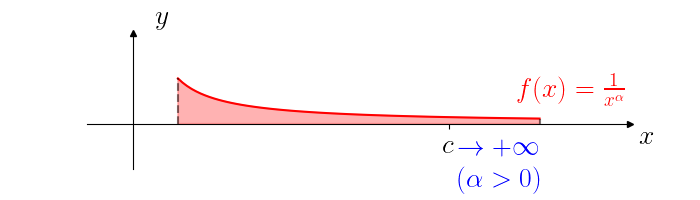
\includegraphics[width=\linewidth]{integrali_impropri/pag77}
		\label{fig:pag77}
	\end{center}

	Fissato $c > 1$, riesco a definire $\int_{1}^{c} f(x)dx$ perché integro una funzione limitata su un intervallo limitato. Posso dunque definire
	\begin{align*}
		\int_{1}^{+\infty} f(x) \ \mathrm{d}x 
		&= \lim_{c\rightarrow +\infty} \int_{1}^{c}f(x) \ \mathrm{d}x \qquad \text{se esiste}
		\\
		\int_{1}^{+\infty} \frac{1}{x^\alpha} dx 
		&= \lim_{c \rightarrow + \infty} \int_{1}^{c} \frac{1}{x^\alpha} \ \mathrm{d} x 
		\\
		&=
		\begin{cases}
			\lim_{c \rightarrow +\infty}\frac{1}{1-\alpha}[c^{1-\alpha}-1] & \text{se } \alpha \neq 1
			\\[1em]
			\lim_{c \rightarrow +\infty} \ln c & \text{se } \alpha=1
		\end{cases}
		\\
		&=
		\begin{cases}
			 \frac{1}{\alpha-1} & \text{se } \alpha > 1
			\\[1em]
			+\infty & \text{se } \alpha \leq 1
		\end{cases}
	\end{align*}
\end{example}
\end{exbar}

	
\begin{exbar}
\begin{example}
	\begin{equation*}
		f(x)=-\ln x, \qquad x \in ]0,1]
	\end{equation*}
	
	e provo a definire 
	\begin{equation*}
		\int_{0}^{1} f(x) \ \mathrm{d}x
	\end{equation*}
	
	cioè l'integrale di una funzione illimitata $\left( \lim_{x \rightarrow 0^+} f(x) = + \infty \right)$ su un intervallo limitato.
	\begin{center}
		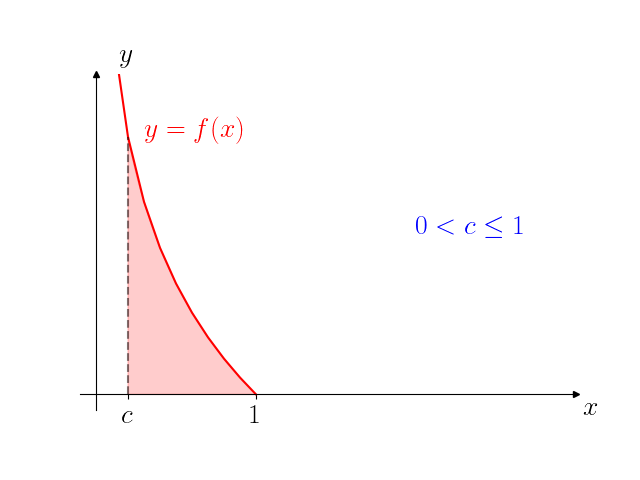
\includegraphics[width=0.75\linewidth]{integrali_impropri/pag79}
		\label{fig:pag79}
	\end{center}
	
	Riesco a definire bene $\int_{c}^{1} f(x) \ \mathrm{d}x$ perché integro una funzione limitata
	$\left( |f(x)|\leq -\ln c \quad \forall \ x \in [c,1] \right)$ su un intervallo limitato.
	
	Posso dunque definire
	\begin{align*}
		\int_{0}^{1} f(x)dx 
		&= \lim_{c\rightarrow +0^+} \int_{c}^{1} f(x) \ \mathrm{d}x \qquad \text{se esiste}
		\\
		\int_{0}^{1}(-\ln x) \ \mathrm{d}x 
		&= \lim_{c \rightarrow 0^+} \int_{c}^{1} (-\ln x) \ \mathrm{d} x
		\\
		&= \lim_{c \rightarrow 0^+} [x-x\ln x]_{c}^{1} 
		\\
		&= \lim_{c \rightarrow 0^+} [1-c+c\ln c]=1
	\end{align*}
\end{example}
\end{exbar}

\begin{definition}
	Sia $f:[a,b[ \ \rightarrow \mathbb{R}; b \in \mathbb{R} \cup\{+\infty\}$ (voglio definire $\int_{a}^{b}f(x) \ \mathrm{d}x$) Riemann integrabile in $[a,c] \ \forall c \in [a,b[$. Se $\exists$ finito il $\lim_{c \rightarrow b^-} \int_{a}^{c} f(x) \ \mathrm{d}x $, allora $f$ si dice integrale in senso improprio o generalizzato in $[a,b[$ e la quantità 
	\begin{equation*}
		\int_{a}^{b} f(x) \ \mathrm{d} x = \lim_{c\rightarrow b^-} \int_{a}^{c} f(x) \ \mathrm{d} x
	\end{equation*}
	si dice integrale improprio o generalizzato di $f$ in $[a,b[$.
	
	Analogamente, data $f:]a,b]\rightarrow \mathbb{R}; a \in \mathbb{R} \cup \{-\infty\}$, Riemann integrabile in $[c,b] \ \forall c \in ]a,b]$. Se $\exists$ finito il $\lim_{c \rightarrow a^+} \int_{c}^{b} f(x) \ \mathrm{d}x$, allora $f$ si dice integrabile in senso improprio o generalizzato in $]a,b]$ e la quantità
	\begin{equation*}
		\int_{a}^{b} f(x) \ \mathrm{d}x = \lim_{c \rightarrow a^+} \int_{c}^{b} f(x) \ \mathrm{d}x
	\end{equation*}
	si dice integrale improprio o generalizzato di $f$ in $]a,b]$.
	
	Se $f$ è integrabile in senso improprio in un intervallo $I$, allora si dice anche che l'integrale (improprio) di $f$ in $I$ è convergente o che $f$ ha integrale (improprio) convergente in $I$.
	
	Se il limite che definisce l'integrale improprio di $f$ è infinito, si dice anche che l'integrale (improprio) di $f$ è divergente o che $f$ ha integrale (improprio) divergente in $I$.
\end{definition}

\begin{attbar}
		Vista la definizione, 
	\begin{equation*}
		\int_{1}^{+\infty} \frac{1}{x^\alpha} \ \mathrm{d}x \text{ converge} \iff \alpha > 1
	\end{equation*}
\end{attbar}

\begin{exbar}
\begin{example} \textbf{importante}
	\begin{align*}
		f(x)=\frac{1}{(x-a)^\alpha}, \qquad
		& x \in ]a, a+1], 
		\\ & a \in \mathbb{R} \text{ fissato}
		\\ & \alpha \in \mathbb{R} \text{ parametro}
		\\ & \alpha > 0
	\end{align*}
	
	Studiamo la convergenza di 
	\begin{align*}
		\int_{a}^{a+1} \frac{1}{(x-a)^\alpha} \ \mathrm{d}x  
		&= \lim_{c \rightarrow a^+} \int_{c}^{a+1} \frac{1}{(x-a)^\alpha} \ \mathrm{d}x
		\\
		&=
		\begin{cases}
			\lim_{c \rightarrow a^+} \frac{1}{1-\alpha} \left[1 - (c-a)^{1-\alpha} \right] & \text{se } \alpha \neq 1 
			\\[1em]
			\lim_{c \rightarrow a^+} -\ln(c-a) & \text{se } \alpha =1
		\end{cases}\\
		&=
		\begin{cases}
			\frac{1}{1-\alpha} & \text{se } \alpha <1 
			\\[1em]
			+\infty & \text{se } \alpha \geq1.
		\end{cases}
	\end{align*}
\end{example}
\end{exbar}

\begin{attbar}
	\begin{equation*}
		\int_{a}^{a+1} \frac{1}{(x-a)^\alpha} \ \mathrm{d}x \text{ converge} \iff \alpha < 1
	\end{equation*}
	
	In particolare
	\begin{equation*}
		\int_{0}^{1} \frac{1}{x^\alpha} \mathrm{d}x \text{ converge} \iff \alpha < 1
	\end{equation*}
\end{attbar}

\begin{exbar}
\begin{example}
	Stabilire se converge 
	\begin{equation*}
		\label{eq:pag 83}
		\int_{0}^{1} \frac{\sin{\frac{1}{x}}}{x^2} \ \mathrm{d}x
	\end{equation*}
	
	\begin{center}
		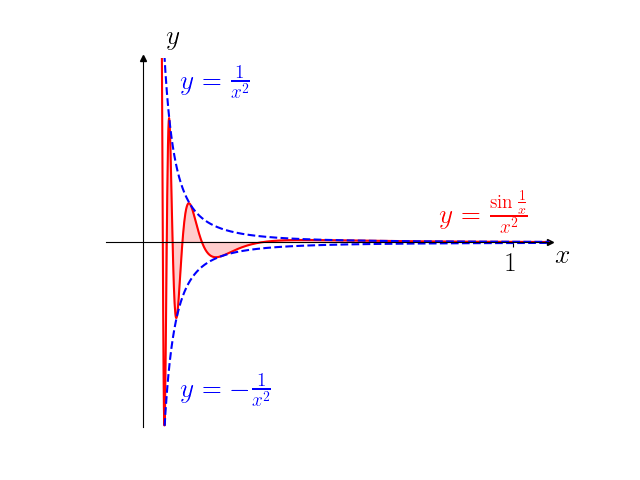
\includegraphics[width=0.75\linewidth]{integrali_impropri/pag83}
		\label{fig:pag83}
	\end{center}
	
		Devo calcolare 
	\begin{equation*}
		\lim_{c\rightarrow0^+} \int_{c}^{1} \frac{\sin{\frac{1}{x}}}{x^2} \ \mathrm{d}x= \lim_{c \rightarrow 0^+} \cos{\frac{1}{x}} \bigg|_{c}^{1}=\lim_{c\rightarrow 0^+}\left(1-\cos{\frac{1}{c}}\right)
	\end{equation*}
	
	che non esiste $\Rightarrow$ la funzione $f(x)=\frac{\sin{\frac{1}{x}}}{x^2}$, non è integrabile in senso improprio in $]0,1]$	
\end{example}
\end{exbar}

\begin{exbar}
\begin{example} \textbf{importante}
	\begin{align*}
		\int_{0}^{+\infty} e^{\alpha x} \ \mathrm{d}x 
		&= \lim_{c \rightarrow +\infty} \int_{0}^{c} e^{\alpha x} \ \mathrm{d}x 
		\\ & =^{\myarrow[10] \alpha \neq 0} \lim_{c \rightarrow +\infty} \frac{1}{\alpha} \ (e^{\alpha c}-1)
		\\
		&= \begin{cases}
			-\frac{1}{\alpha} & \text{se } \alpha <0
			\\
			+\infty & \text{se } \alpha >0.
		\end{cases}
	\end{align*}
\end{example}
\end{exbar}

\begin{attbar}
	\begin{equation*}
		\int_{0}^{+\infty} e^{\alpha x} \ \mathrm{d}x \text{ converge } \iff \alpha < 0
	\end{equation*}
	
	Analogamente
	\begin{equation*}
		\int_{-\infty}^{0} e^{\alpha x} \ \mathrm{d}x \text{ converge } \iff  \alpha > 0
	\end{equation*}
\end{attbar}

Dato $ a>0$, scrivendo $e^{\alpha x} = e^{(\alpha \ln a)x}$ si studia la convergenza degli integrali
\begin{equation*}
	\int_{-\infty}^{0} e^{\alpha x} \ \mathrm{d}x \qquad \int_{0}^{+\infty}  e^{\alpha x} \ \mathrm{d}x.
\end{equation*}

(Utile esercizio per casa)


\textbf{Nota Bene}

$f:[1,+\infty[ \ \rightarrow \mathbb{R}$ continua. E' vero o falso che $\lim_{x \rightarrow +\infty} f(x)=0 \Rightarrow \int_{1}^{+\infty} f(x) \ \mathrm{d}x$ converge?

\begin{center}
	\textbf{È falso!!!} Si veda $f(x)=\frac{1}{x}$
\end{center}

E' vero o falso che
$\int_{1}^{+\infty}f(x) \ \mathrm{d}x$ converge $\Rightarrow \lim_{x \rightarrow +\infty} f(x) = 0$?

\begin{center}
	\textbf{È falso!!!}
\end{center}

\begin{center}
	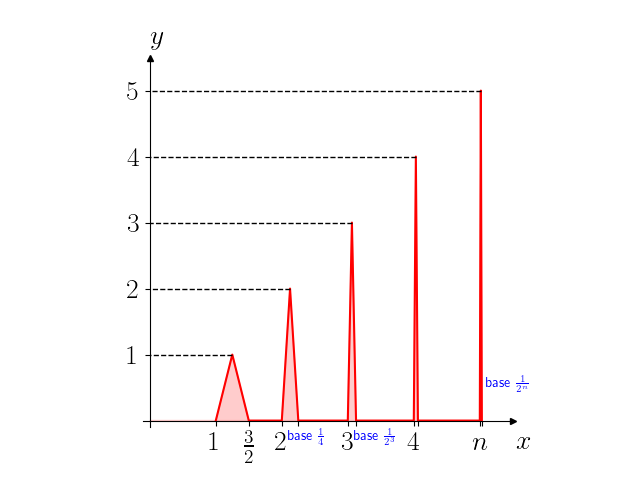
\includegraphics[width=0.75\linewidth]{integrali_impropri/pag85}
	\label{fig:pag85}
\end{center}

Ad ogni numero naturale $n$ costruite un triangolo di base $\frac{1}{2^n}$ e altezza $n$
\begin{equation*}
	\int_{1}^{+\infty} f(x) \ \mathrm{d}x = \sum (\text{aree dei triangoli}) = \sum_{n=1}^{\infty} \frac{1}{2} \frac{1}{2^n} \cdot n = \frac{1}{2} \sum_{n=1}^{\infty} \frac{n}{2^n}, 
\end{equation*}

che è una serie convergente.


\begin{attbar}
	Se $f:[a,b] \rightarrow \mathbb{R}$ è Riemann integrabile, allora è integrabile anche in senso improprio e i due integrali coincidono.
\end{attbar}


\begin{definition}
	$f:[a,b] \ \rightarrow \mathbb{R}, \; a,b \in \mathbb{R} \cup \{\pm \infty\}$, Riemann integrabile in $[c,d] \ \forall \ a < c < d < b$. $f$ si dice integrabile in senso improprio in $ ]a,b[$ se, fissato $\xi \in \ ]a,b[$, lo è in $]a, \xi]$ e in $[\xi,b[$ $\bigg($esistono finiti $\lim_{c \rightarrow a^+} \int_{c}^{\xi} f(x) \ \mathrm{d}x$ e $\lim_{d \rightarrow b^-} \int_{\xi}^{d} f(x) \ \mathrm{d}x \bigg)$ e in tal caso si pone 
	\begin{equation*}
		\int_{a}^{b} f(x)dx = \int_{a}^{\xi} f(x)dx + \int_{\xi}^{b} f(x) dx
	\end{equation*}
	
	Si verifica che la definizione non dipende da punto $\xi$ fissato.
\end{definition}


\begin{exbar}
\begin{example}
	Come si integra $\int_{-\infty}^{+\infty} \frac{1}{1+x^2} \ \mathrm{d}x$?
	
	$x \mapsto \frac{1}{1+x^2}$ è integrabile secondo Riemann in $[c,d] \ \forall  \ c < d$. 
	
	Sia $\xi = 2$. Dobbiamo verificare se la funzione è integrabile in senso improprio in $]-\infty,2] $ e in $ [2, +\infty[$
	\begin{gather*}
		\int_{-\infty}^{2} \frac{1}{1+x^2} \ \mathrm{d}x = \lim_{c \rightarrow -\infty} \int_{c}^{2} \frac{1}{1+x^2} \ \mathrm{d}x = \lim_{c \rightarrow -\infty} \left( \arctan{2 + \frac{\pi}{2}} \right)= \arctan{2 + \frac{\pi}{2}}
		\\
		\int_{2}^{+\infty} \frac{1}{1 + x^2} \ \mathrm{d}x = \lim_{c \rightarrow +\infty} \int_{2}^{c} \frac{1}{1 + x^2} \mathrm{d}x = \lim_{c \rightarrow +\infty} (\arctan{c} - \arctan{2}) = \frac{\pi}{2} - \arctan{2}
		\\
		\Rightarrow \int_{-\infty}^{+\infty} \frac{1}{1+x^2} \ \mathrm{d}x \text{ converge e } \int_{-\infty}^{+\infty} \frac{1}{1+x^2} \ \mathrm{d}x = \int_{-\infty}^{2} \frac{1}{1+x^2} \ \mathrm{d}x + \int_{2}^{+\infty} \frac{1}{1+x^2} \ \mathrm{d}x
	\end{gather*}
\end{example}
\end{exbar}


\begin{exbar}
\begin{example}
	\begin{gather*}
		f(x)=\frac{1}{x^\alpha}, \qquad x \in \ ]0,+\infty[
		\\
		\alpha > 0 \Rightarrow \lim_{x \rightarrow 0^+} f(x)=+\infty.
	\end{gather*}
	
	Preso $\xi=1$, $f$ è integrabile in senso improprio in $]0,+\infty[ \ \iff$ entrambi gli integrali $\int_{0}^{1} \frac{1}{x^\alpha} \ \mathrm{d}x$ e $\int_{1}^{+\infty} \frac{1}{x^\alpha} \ \mathrm{d}x$ convergono. Ma
	\begin{gather*}
		\int_{0}^{1} \frac{1}{x^\alpha} \ \mathrm{d}x \text{ converge} \iff \alpha < 1 
		\\
		\int_{1}^{+\infty} \frac{1}{x^\alpha} \ \mathrm{d}x \text{ converge} \iff \alpha > 1
		\\
		\Rightarrow \int_{0}^{+\infty} \frac{1}{x^\alpha} \ \mathrm{d}x \text{ non converge per alcun valore di } \alpha
	\end{gather*}
\end{example}
\end{exbar}


\begin{exbar}
\begin{example}
	\begin{equation*}
		f(x)= 
		\begin{cases}
			e^x & \text{se } x \leq 1 
			\\
			\frac{1}{x \sqrt{x-1}} & \text{se } x>1
		\end{cases}
	\end{equation*}
	
	vogliamo stabilire se $\int_{-\infty}^{+\infty} f(x) \ \mathrm{d}x$ converge.
	\begin{center}
		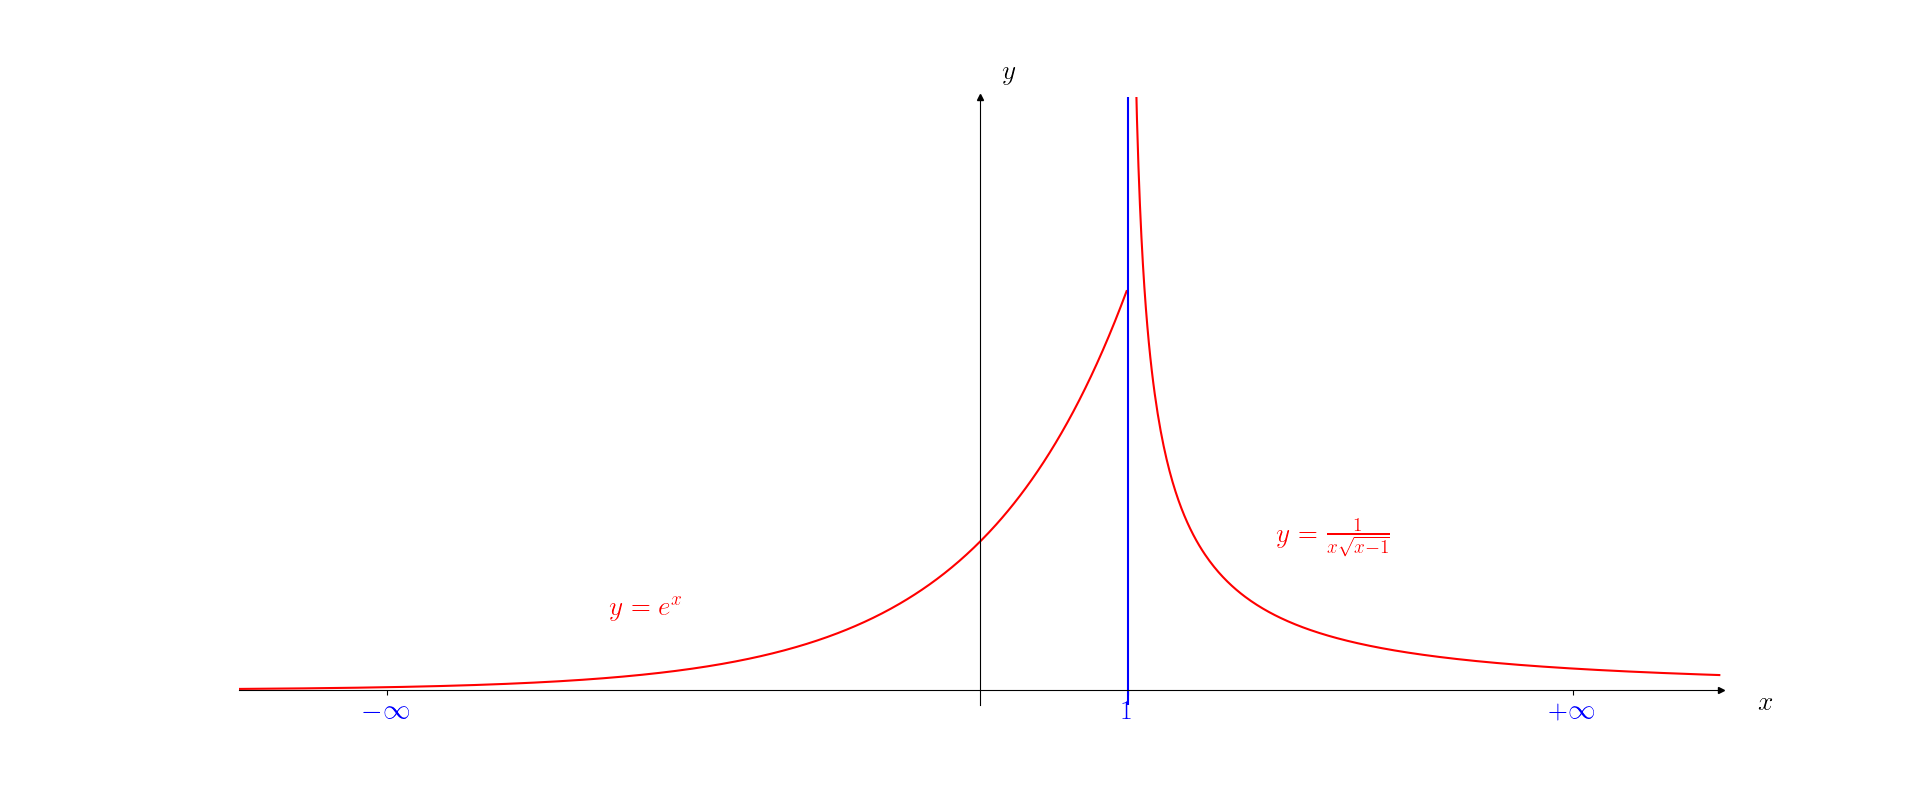
\includegraphics[width=0.75\linewidth]{integrali_impropri/pag89}
		\label{fig:pag89}
	\end{center}
	
	Devo studiare $\int_{-\infty}^{1} f(x) \ \mathrm{d}x = \int_{-\infty}^{1} e^x \ \mathrm{d}x$ e, prendendo $\xi=3$,  $\int_{1}^{3} f(x) \ \mathrm{d}x$ e $\int_{3}^{+\infty} f(x) \ \mathrm{d}x$. Se tutti convergono, anche $\int_{-\infty}^{+\infty} f(x) \ \mathrm{d}x$ converge e 
	\begin{equation*}
		\int_{-\infty}^{+\infty} f(x) \ \mathrm{d}x = \int_{-\infty}^{1} f(x) \ \mathrm{d}x + \int_{1}^{3} f(x) \ \mathrm{d}x + \int_{3}^{+\infty} f(x) \ \mathrm{d}x
	\end{equation*}
\end{example}
\end{exbar}

In generale, data $f:]a,b[ \ \rightarrow \mathbb{R}$ integrabile in senso improprio in $]x_0,x_1[, \ ]x_1,x_2[, \ \ldots, \ ]x_{n-1}, \ x_n[$ con $a = x_0 < x_1 < \ldots < x_n = b$, allora $f$ si dice integrabile in senso improprio in $]a,b[$ e si pone 
\begin{equation*}
	\int_{a}^{b} f(x) \ \mathrm{d}x= \sum_{i=1}^{n} \int_{x_{i-1}}^{x_i} f(x) \ \mathrm{d}x.
\end{equation*}

\subsection{Criteri di integrabilità}
\begin{proposition}
	\label{pr: integrabilità definita}
	Sia $f:[a,b[ \ \rightarrow \mathbb{R}, \ b \in \mathbb{R} \cup \{+\infty\}$ tale che $f(x) \geq 0$ definitivamente per $x \rightarrow b^-$ e tale che sia Riemann integrabile in $[a,b] \ \forall c \in [a,b[$. Allora esiste
	\begin{equation*}
		\lim_{c \rightarrow b^-} \int_{a}^{c} f(x) \ \mathrm{d}x
 	\end{equation*}
	cioè l'integrale improprio $\int_{a}^{b} f(x) \ \mathrm{d}x$ è ben definito (converge o diverge a $+\infty$).
\end{proposition}

\begin{dembar}
	\textbf{Dimostrazione} della \textbf{Proposizione \ref{pr: integrabilità definita}}
	
	
	Per semplicità assumiamo $f(x) \geq 0 \ \forall \ x \in [a,b[$. Sia allora $F(c)=\int_{a}^{c} f(x) \ \mathrm{d}x, \ c \in [a,b[$. 
	
	Allora $F$ è monotona crescente, dunque, presi $c_2 > c_1$ si ha
	\begin{equation*}
		F(c_2) - F(c_1) = \int_{a}^{c_2} f(x) \ \mathrm{d}x - \int_{a}^{c_1} f(x) \ \mathrm{d}x = \int_{c_1}^{c_2} f(x) \ \mathrm{d}x \geq 0
	\end{equation*}
	
	perché $f(x) \geq 0 \ \forall x \in [c_1,c_2] \Rightarrow F(c_2) \geq F_{c_1}$.
	
	$F$ ha limite per $c \rightarrow b^-$, cioè esiste
	\begin{equation*}
		\lim_{c \rightarrow b^-} F(c) = \lim_{c \rightarrow b^-} \int_{a}^{b} f(x) \ \mathrm{d}x.
	\end{equation*}
	
	Un risultato analogo si enuncia per funzioni definitivamente $\leq 0$ per $ x \rightarrow b^-$ o per una funzione $f: \ ]a,b] \rightarrow \mathbb{R}, \ a \in \mathbb{R} \cup \{-\infty\}. \ \square$ 
\end{dembar}


Come per le serie ci concentriamo su criteri di integrabilità per funzioni di segno definito.

\subsubsection{Criterio del confronto}
\begin{theorem} (criterio del confronto)
	
\end{theorem}
	\label{th:criterio del confronto integrale}
	$f,g : [a,b[ \ \rightarrow \mathbb{R}, \ b \in \mathbb{R} \cup \{+\infty\}$, Riemann integrabili in $[a,c] \ \forall c \in [a,b[$ e tali che $0 \leq f(x) \leq g(x)$ definitivamente per $x \rightarrow b^-$.
	\begin{enumerate}
		\item Se $\int_{a}^{b} g(x) \ \mathrm{d}x$ converge, allora converge anche $\int_{a}^{b} f(x) \ \mathrm{d}x$.
		\item Se $\int_{a}^{b} f(x) \ \mathrm{d}x$ diverge, allora diverge anche $\int_{a}^{b} g(x) \ \mathrm{d}x$.
	\end{enumerate}
	Un risultato analogo vale per funzioni $f,g: \ ]a,b] \rightarrow \mathbb{R}, \ a \in \mathbb{R} \cup \{-\infty\}$, con ovvie modifiche.


\begin{dembar}
		\textbf{Dimostrazione} del \textbf{Teorema \ref{th:criterio del confronto integrale}}
		
		Per semplicità assumiamo $0 \leq f(x) \leq g(x) \ \forall \ x \in [a,b[$.
		\begin{enumerate}
			\item $\exists$ finito $\lim_{c \rightarrow b^-} \int_{a}^{c} g(x) \ \mathrm{d}x \ \forall \ c \in [a,b[, \ \int_{a}^{c} f(x) \ \mathrm{d}x \leq \int_{a}^{c} g(x) \ \mathrm{d}x$ perché $f(x) \leq g(x)$. Allora 
			\begin{equation*}
				\undercomment{\lim_{c \rightarrow b^-} \int_{a}^{c} f(x) \ \mathrm{d}x} {\text{esiste perché}} {f(x) \geq 0} \leq \lim_{c \rightarrow b^-} \int_{a}^{c} g(x) \ \mathrm{d}x
			\end{equation*}
			
			e quindi $\lim_{c \rightarrow b^-} \int_{a}^{c} f(x) \ \mathrm{d}x $ esiste finito e $\int_{a}^{b} f(x) \ \mathrm{d}x$ è convergente.
			
			\item $\lim_{c \rightarrow b^-} \int_{a}^{c} f(x) \ \mathrm{d}x = +\infty $ ($f(x)\geq 0$)
			\begin{gather*}
				\int_{a}^{c} g(x) \ \mathrm{d}x \geq \uppercomment{\int_{a}^{c} f(x) \ \mathrm{d}x} {\rightarrow +\infty} {\text{per } c \rightarrow + \infty} \ \forall \ c \in [a,b[
				\\
				\Rightarrow \lim_{c \rightarrow b^-} \int_{a}^{c} g(x) \ \mathrm{d}x = +\infty
			\end{gather*}
			 
			per il teorema del confronto sui limiti. $\square$
		\end{enumerate}
\end{dembar}


\subsubsection{Criterio di assoluta integrabilità}
\begin{theorem}
	\label{th:criterio assoluta integrabilità}
	$f:[a,b[ \ \rightarrow \mathbb{R}, \ b \in \mathbb{R} \cup \{+\infty\}$ Riemann integrabile in $[a,c] \ \forall \ c \in [a,b[$ e tale che $|f|$ è integrabile in senso improprio in $[a,b[$ (si dice che l'integrale improprio di $f$ è assolutamente convergente o che converge assolutamente). Allora $\int_{a}^{b} f(x) \ \mathrm{d}x$ converge.
\end{theorem}


\begin{dembar}
	\textbf{Dimostrazione} del \textbf{Teorema \ref{th:criterio assoluta integrabilità}}
	
	\begin{gather*}
		f = f^+ - f^-
		\\
		f^+ = \max \{f(x), 0\} \geq 0 \quad f^- =\min \{f(x), 0\} \geq 0 \quad \forall \ x
		\\
		\left| f(x) \right| = f^+(x) + f^-(x)
	\end{gather*}
	\begin{center}
		\includegraphics[width=0.75\linewidth]{integrali_impropri/pag94(2)}
		\label{fig:pag94}
	\end{center}

	$f^+$ e $f^-$ sono Riemann integrabili  in  $[a,c] \ \forall \ c \in [a,b[$ e inoltre
	\begin{equation*}
		\begin{array}{c}
			0 \leq f^+(x) \leq |f(x)|
			\\
			0 \leq f^-(x) \leq |f(x)|
		\end{array}
		\qquad \forall \ x \in [a,b[
	\end{equation*}
	$\Rightarrow$ per il criterio del confronto $\int_{a}^{b} f^+(x) \ \mathrm{d}x$ e $\int_{a}^{b} f^-(x) \ \mathrm{d}x$ convergono entrambi 
	\begin{equation*}
		\Rightarrow \lim_{c \rightarrow b^-} \int_{a}^{c} f(x) \ \mathrm{d}x = \lim_{c \rightarrow b^-} \left[ \int_{a}^{c}f^+(x) \ \mathrm{d}x - \int_{a}^{c}f^-(x) \ \mathrm{d}x \right]
	\end{equation*}
	esiste finito per il teorema sulla somma dei limiti $\Rightarrow \int_{a}^{b} f(x) \ \mathrm{d}x$ converge. $\square$
\end{dembar}


\begin{attbar}
	Sia $f: [a,b[ \rightarrow \mathbb{R}, \ b \in \mathbb{R} \cup \{+\infty\}$ e se $\int_{a}^{b} f(x) \ \mathrm{d}x$ converge, non è detto che $\int_{a}^{b} |f(x)| \ \mathrm{d}x$ converga.
\end{attbar}


\begin{exbar}
\begin{example}
	\begin{equation*}
		f(x) = \frac{\sin x}{x}, \qquad x \geq 1
	\end{equation*}
	
	e dimostriamo che $ \int_{1}^{+\infty} \frac{\sin x}{x} \ \mathrm{d}x$ converge. Fissiamo $c>1$
	\begin{gather*}
		\int_{1}^{c} \frac{\sin x}{x} \ \mathrm{d}x= -\frac{\cos x}{x} \bigg|_{1}^{c} - \int_{1}^{c} \frac{\cos x}{x^2} \ \mathrm{d}x = \cos 1 - \frac{\cos c}{c} - \int_{1}^{c} \frac{\cos x}{x^2} \ \mathrm{d}x
		\\
		\lim_{c \rightarrow +\infty} \int_{1}^{c} \frac{\sin x}{x} \ \mathrm{d}x = \lim_{c \rightarrow +\infty} \left[\cos 1 - \uppercomment{\frac{\cos c}{c}} {0} {\myarrow[90]} - \lowercomment{\int_{1}^{c} \frac{cosx}{x^2} \ \mathrm{d}x} {\lim_{c \rightarrow + \infty} \int_{1}^{c} \frac{\cos x}{x^2} \ \mathrm{d}x} {\text{esiste finito}}\right] 
	\end{gather*}

	
	$\frac{|\cos x|}{x^2} \leq \frac{1}{x^2} \ \forall \ x \geq 1$ e $ \int_{1}^{+\infty} \frac{1}{x^2} \ \mathrm{d}x$ converge 
	
	$\Rightarrow \int_{1}^{+\infty} \frac{|\cos x|}{x^2} \ \mathrm{d}x$ converge per il criterio del confronto 
	
	$\Rightarrow \int_{1}^{+\infty} \frac{\cos x}{x^2} \ \mathrm{d}x$ converge per il criterio di assoluta integrabilità
	
	$\Rightarrow \lim_{c \rightarrow +\infty} \int_{1}^{c} \frac{\sin x}{x} \ \mathrm{d}x = \cos 1 - \int_{1}^{+\infty} \frac{\cos x}{x^2} \ \mathrm{d}x$ esiste finito e dunque $\int_{1}^{+\infty} \frac{\sin x}{x} \ \mathrm{d}x$ converge 
	\\[1em]

	Ma $\int_{1}^{+\infty} |\frac{\sin x}{x}|dx =+\infty$.
	
	Presi $k \geq 1, \ k \in \mathbb{N}$
	\begin{gather*}
		k\pi \leq x \leq (k+1)\pi
		\\
		\frac{1}{(k+1)\pi} \leq \frac{1}{x} \leq \frac{1}{k\pi}
		\\
		\int_{k\pi}^{(k+1)\pi} \frac{(\sin x)}{x} \ \mathrm{d}x \geq \int_{k\pi}^{(k+1)\pi} \frac{1}{(k+1)\pi} (\sin x) \ \mathrm{d}x = \frac{2}{(k+1)\pi} 
		\\
		\int_{1}^{+\infty} \frac{|\sin{x}|}{x} \ \mathrm{d}x \geq \sum_{k=1}^{\infty} \int_{k\pi}^{(k+1)\pi} \frac{|\sin{x}|}{x} \ \mathrm{d}x \geq \sum_{k=1}^{\infty} \frac{2}{(k+1)\pi}=+\infty
	\end{gather*}
	
	perché $\frac{2}{(k+1)\pi} \sim \frac{1}{k}$.
\end{example}
\end{exbar}


\subsubsection{Criterio asintotico del confronto}
\begin{theorem}
	\label{th:criterio asintotico confronto integrale}
	$f,g: [a,b[\rightarrow \mathbb{R}, \ b \in \mathbb{R} \cup \{+\infty\}$, Riemann integrabili in $[a,c] \ \forall c \in [a,b[$ tali che $f(x),g(x)\geq 0$ definitivamente per $x \rightarrow b^-$ e $\lim_{x \rightarrow b^-} \frac{f(x)}{g(x)}= \ell \in [0,+\infty[$
	\begin{enumerate}
		\item Se $\ell \in \ ]0,+\infty[$, allora $ \int_{a}^{b} f(x) \ \mathrm{d}x$ converge $\iff \int_{a}^{b} g(x) \ \mathrm{d}x$ converge.
		
		\item Se $\ell=0$ e $\int_{a}^{b} g(x) \ \mathrm{d}x $ converge, allora $\int_{a}^{b} f(x) \ \mathrm{d}x$ converge.
		
		\item Se $\ell=+\infty$ e $\int_{a}^{b} g(x) \ \mathrm{d}x$ diverge, allora $\int_{a}^{b} f(x) \ \mathrm{d}x$ diverge.
	\end{enumerate}
\end{theorem}


\begin{dembar}
\textbf{Dimostrazione} del \textbf{Teorema \ref{th:criterio asintotico confronto integrale}}
\begin{enumerate}
	\item $\lim_{x \rightarrow b^-} \frac{f(x)}{g(x)} = \ell \in \ ]0,+\infty[$ 
	allora $\frac{\ell}{2} \leq \frac{f(x)}{g(x)} \leq 2\ell$ definitivamente per $x \rightarrow b^-$ perché $]\frac{\ell}{2},2\ell[$ è un intorno di $\ell$. 
	\begin{equation*}
	\begin{array}{c c}
		f(x) \leq 2 \ell g(x) & \text{definitivamente}
		\\
		g(x) \leq \frac{2}{\ell} f(x) & \text{per } x \rightarrow b^-
	\end{array} 
	\end{equation*}
	 
	Se $\int_{a}^{b} g(x) \ \mathrm{d}x$ converge $\Rightarrow \int_{a}^{b} f(x) \ \mathrm{d}x$ converge;
	
	se $\int_{a}^{b} f(x) \ \mathrm{
	d}x$ converge $\Rightarrow \int_{a}^{b} g(x) \ \mathrm{d}x$ converge per il criterio del confronto.
	
	\item $\lim_{x \rightarrow b^-} \frac{f(x)}{g(x)} = 0 \Rightarrow \frac{f(x)}{g(x)} \leq 1 $ definitivamente per $x\rightarrow b^-$ 
	
	$\Rightarrow f(x) \leq g(x)$ definitivamente per $x\rightarrow b^- \Rightarrow $ 
	
	$\Rightarrow$ se $\int_{a}^{b} g(x) \ \mathrm{d}x$ converge, allora $\int_{a}^{b} f(x) \ \mathrm{d}x$ converge per il criterio del confronto.
	
	\item $\lim_{x \rightarrow b^-} \frac{f(x)}{g(x)} = +\infty \Rightarrow \frac{f(x)}{g(x)} \geq 1$ definitivamente per $x \rightarrow b^-$ 
	
	$\Rightarrow f(x) \geq g(x)$ definitivamente per $x \rightarrow b^-$ 
	
	$\Rightarrow$ se $\int_{a}^{b} g(x) \ \mathrm{d}x$ diverge, allora $\int_{a}^{b} f(x) \ \mathrm{d}x$ diverge sempre per il criterio del confronto. $\square$
\end{enumerate}
\end{dembar}


\begin{exbar}
\begin{example} \textbf{importante}
	
	Studiamo la convergenza di 
	\begin{equation*}
		\int_{2}^{+\infty} \frac{1}{x^\alpha (\ln x)^\beta} \ \mathrm{d}x, \qquad \alpha,\beta \in \mathbb{R}
	\end{equation*}
	\begin{itemize}
		\item Se $\alpha > 1 $
		\begin{equation*}
			\int_{2}^{+\infty}\frac{1}{x^\alpha} \ \mathrm{d}x \text{ converge}
		\end{equation*}

		
		\begin{itemize}
			\item Se $\beta \geq 0 $
			\begin{gather*}
				\frac{1}{x^\alpha (\ln x)^\beta} \leq \frac{1}{x^\alpha} \text{ per } x > a
				\\
				\Rightarrow \int_{2}^{+\infty} \frac{1}{x^\alpha(\ln x)^\beta} \ \mathrm{d}x \text{ converge}
			\end{gather*}
			
			\item Se $\beta < 0 $
			\begin{equation*}
				\frac{1}{x^\alpha(\ln x)^\beta} = \frac{(\ln x)^{-\beta}}{x^\alpha}
			\end{equation*}
			
			Preso $\epsilon > 0$ si ha $\ln x \leq x^\epsilon$ definitivamente per $x \rightarrow+\infty$ 
			\begin{equation*}
				\frac{(\ln x)^{-\beta}}{x^\alpha} \leq \frac{x^{-\epsilon \beta}}{x^\alpha}=\frac{1}{x^{\alpha+\epsilon\beta}}
			\end{equation*}
			
			definitivamente per $x\rightarrow +\infty$.
			
			Scelgo $\epsilon$ in modo che $\alpha + \epsilon\beta > 1$, cioè $\epsilon < \uppercomment{\frac{1-\alpha}{\beta}} {} { >0}$
			\begin{gather*}
				\Rightarrow \int_{2}^{+\infty} \frac{1}{x^{\alpha+\epsilon\beta}} \ \mathrm{d}x \text{ converge}
				\\
				\Rightarrow \int_{2}^{+\infty} \frac{1}{x^\alpha(\ln x)^\beta} \ \mathrm{d}x \text{ converge.}
			\end{gather*}
		\end{itemize}
		
		\item Se $\alpha < 1 $
		\begin{equation*}
			\int_{2}^{+\infty} \frac{1}{x^\alpha} \ \mathrm{d}x \text{ diverge}
		\end{equation*}

		\begin{itemize}
			\item Se $\beta \geq 0 $ 
			\begin{gather*}
				\frac{1}{x^\alpha(\ln x)^\beta }\geq \uppercomment{??} {\text{integrale}} {\text{divergente}} 
				\\
				\frac{1}{x^\alpha(\ln x)^\beta} = \frac{(\ln x)^{-\beta}}{x^\alpha}.
			\end{gather*}

			Fissato $\epsilon>0, \ \ln x \leq x^\epsilon $ definitivamente per $x \rightarrow +\infty$ 
			
			$(\ln x)^{-\beta} \undercomment{\geq} {-\beta < 0} {} x^{-\epsilon\beta}$ definitivamente per $x \rightarrow +\infty$ 
			
			$\frac{1}{x^\alpha (\ln x)^\beta} \geq \frac{x^{-\epsilon\beta}}{x^\alpha} = \frac{1}{x^{\alpha+\epsilon\beta}}$ definitivamente per $x \rightarrow +\infty$.
			
			Scelgo  $\epsilon$ in modo che $ \alpha + \epsilon\beta < 1, \ \epsilon < \frac{1-\alpha}{\beta} $
			
			\begin{gather*}
				\Rightarrow \int_{2}^{+\infty} \frac{1}{x^{\alpha + \epsilon\beta}} \ \mathrm{d}x \text{ diverge}
				\\
				\Rightarrow \int_{2}^{+\infty} \frac{1}{x^\alpha(\ln x)^\beta} \ \mathrm{d}x 
			\end{gather*}
		
			diverge per il criterio del confronto.
			
			\item  Se $\beta \leq 0 $
			\begin{gather*}
				\frac{1}{x^\alpha(\ln x)^\beta} = \frac{(\ln x)^{-\beta}}{x^\alpha} \undercomment{\geq} {\text{se } x > e} {} \frac{1}{x^\alpha}
				\\
				\int_{2}^{+\infty}\frac{1}{x^\alpha} \ \mathrm{d}x \text{ diverge}
				\\
				\Rightarrow \int_{2}^{+\infty} \frac{1}{x^\alpha (\ln x)^\beta} \ \mathrm{d}x
			\end{gather*}
			
			  diverge per il criterio del confronto.
		\end{itemize}
		
		\item Se $\alpha=1$
		\begin{equation*}
			 \int_{2}^{+\infty} \frac{1}{x(\ln x)^\beta} \ \mathrm{d}x
		\end{equation*}
		\begin{itemize}
			\item Se $\beta=0$
			\begin{equation*}
				\Rightarrow \int_{2}^{+\infty} \frac{1}{x} \ \mathrm{d}x =+\infty
			\end{equation*}
			
			\item Se $\beta \neq 0,1$
			\begin{align*}
				\int_{2}^{+\infty} \frac{1}{x(\ln x)^\beta} \ \mathrm{d}x 
				&= \lim_{c \rightarrow +\infty} \int_{2}^{c} (\ln x)^{-\beta} \frac{1}{x} \ \mathrm{d}x = \lim_{c \rightarrow +\infty} \frac{1}{1-\beta} (\ln x)^{1-\beta} \bigg|_{2}^{c} = 
				\\
				&= 
				\begin{cases}
					\frac{(\ln 2)^{1-\beta}}{\beta - 1} & \text{se } \beta > 1
					\\[1em]
					+\infty & \text{se } \beta < 1
				\end{cases}
			\end{align*}
			
			\item Se $\beta = 1$
			\begin{equation*}
			 	\int_{2}^{+\infty} \frac{1}{x \ln x} \ \mathrm{d}x = \lim_{c \rightarrow +\infty} \int_{2}^{c} \frac{1}{x \ln x} \ \mathrm{d}x = \lim_{c\rightarrow +\infty} \ln(\ln x)\bigg|_{2}^{c} = +\infty
			\end{equation*}
		\end{itemize}
	\end{itemize}	
\end{example}
\end{exbar}


\begin{attbar}
\begin{equation*}
		\int_{2}^{+\infty} \frac{1}{x^\alpha(\ln x)^\beta} \ \mathrm{d}x \text{ converge } \iff \alpha > 1 \text{ o } (\alpha=1 \text{ e } \beta >1)
\end{equation*}
\end{attbar}


\begin{exbar}
\begin{example} \textbf{importante}
	
	Studiamo la convergenza di
	\begin{equation*}
		\int_{0}^{\frac{1}{2}} \frac{1}{x^\alpha |\ln x|^\beta} \ \mathrm{d}x, \qquad \alpha,\beta \in \mathbb{R}
	\end{equation*}
	\begin{align*}
		\int_{0}^{\frac{1}{2}} \frac{1}{x^\alpha|\ln x|^\beta} \ \mathrm{d}x 
		&= \lim_{c \rightarrow 0^+} \int_{c}^{\frac{1}{2}} \frac{1}{x^\alpha |\ln x|^\beta} \ \mathrm{d}x =
		\\
		&\undercomment{=} {t = \frac{1}{x}} {} \lim_{c \rightarrow 0^+} \int_{2}^{\frac{1}{c}} \frac{1}{\frac{1}{t^\alpha} \left| \ln{\frac{1}{t}} \right|^\beta} \left( \frac{1}{t^2} \right) \ \mathrm{d}t =
		\\
		&= \lim_{c \rightarrow 0^+} \int_{2}^{\frac{1}{c}} \frac{1}{t^{2-\alpha} (\ln t)^\beta} \ \mathrm{d}t =
		\\
		&\undercomment{=} {d = \frac{1}{c}} {} \lim_{d \rightarrow +\infty} \int_{2}^{d} \frac{1}{t^{2-\alpha} (\ln t)^\beta} \ \mathrm{d}t =\int_{2}^{+\infty} \frac{1}{t^{2-\alpha}(\ln t)^\beta} \ \mathrm{d}t
	\end{align*}
	che converge $\iff 2-\alpha > 1$ oppure ($2-\alpha = 1$ e $\beta>1$) $\iff \alpha <1 $ oppure ($\alpha =1 \text{ e } \beta>1$)
\end{example}
\end{exbar}

\begin{attbar}
\begin{equation*}
	\int_{0}^{\frac{1}{2}} \frac{1}{x^\alpha |\ln x|^\beta} \ \mathrm{d}x \text{ converge } \iff \alpha < 1 \text{ o } (\alpha=1 \text{ e } \beta >1)
\end{equation*}
\end{attbar}


\begin{exbar}
\begin{example}
	
	Studiare la convergenza dell'integrale improprio
	\begin{equation*}
		\int_{-\infty}^{+\infty} e^{-x^{2}} \ \mathrm{d}x \quad (=\sqrt{\pi})
	\end{equation*}
	
	Devo studiare separatamente 
	\begin{equation*}
		\int_{-\infty}^{0} e^{-x^{2}} \ \mathrm{d}x \qquad \text{e} \qquad \int_{0}^{+\infty} e^{-x^{2}} \ \mathrm{d}x 
	\end{equation*}
	
	e vedere se entrambi convergono. 
	
	$x\mapsto e^{-x^{2}} $ è pari e dunque
	\begin{align*}
		\int_{-\infty}^{0} e^{-x^{2}} \ \mathrm{d}x
		&= \lim_{c \rightarrow -\infty} \int_{c}^{0} e^{-x^{2}} \ \mathrm{d}x \lowercomment{=}{t=-x}{}
		\\
		&= \lim_{c \rightarrow -\infty} \int_{0}^{-c} e^{-t^2} \ \mathrm{d}t \uppercomment{=}{}{d=-c}
		\\
		&= \lim_{d\rightarrow +\infty} \int_{0}^{d} e^{-x^{2}} \ \mathrm{d}x = \int_{0}^{+\infty} e^{-x^{2}} \ \mathrm{d}x
	\end{align*}
	\begin{gather*}
		\int_{-\infty}^{0} e^{-x^{2}} \ \mathrm{d}x \text{ converge } \iff \int_{0}^{+\infty} e^{-x^{2}} \ \mathrm{d}x \text{ converge.}
		\\
		0 \leq e^{-x^2} \leq e^{-x} \ \forall x \geq 1 \text{ e } \int_{0}^{+\infty}e^{-x} \ \mathrm{d}x = 1 \text{ cioè converge}
	\end{gather*}
	
	 $\Rightarrow$ per il criterio del confronto $\int_{0}^{+\infty} e^{-x^2}dx$ converge.
\end{example}
\end{exbar}


\begin{exbar}
\begin{example}
		
	Studiare la convergenza dell'integrale improprio 
	\begin{equation*}
		\int_{1}^{+\infty} \frac{x^\alpha e^{x^4}}{1+e^{4x^4}} \ \mathrm{d}x \qquad \text{ al variare di } \alpha \in \mathbb{R}.
	\end{equation*}
	
	Per $x \rightarrow +\infty$
	\begin{gather*}
		\frac{x^\alpha e^{x^4}}{1+e^{4x^4}} \sim \frac{x^\alpha e^{x^4}}{x^{4x^4}} = x^\alpha e^{-3x^4}
		\\
		\int_{1}^{+\infty}\frac{x^\alpha e^{x^4}}{1+e^{4x^4}} \ \mathrm{d}x \text{ converge } \iff \int_{1}^{+\infty} x^\alpha e^{-3x^4} \ \mathrm{d}x \text{ converge}
	\end{gather*}
	
	(Provare per casa ponendo $x=\ln t$).
	
	Sicuramente $x^\alpha \leq e^{x^4}$ definitivamente per $x \rightarrow +\infty$ e dunque $x^\alpha e^{-3x^4} \leq e^{-2x^4}\leq e^{-x} $ per $x \geq 1$
	
	$\Rightarrow \int_{1}^{+\infty} x^\alpha e^{-3x^4}dx $ converge per il criterio del confronto $\forall \ \alpha \in \mathbb{R}$.
\end{example}
\end{exbar}


\begin{exbar}
\begin{example}
	
	
	Studiare la convergenza di 
	\begin{gather*}
		\int_{0}^{\mathcircled{+\infty}} \lowercomment{\frac{\ln(3 + \sin x)}{\sqrt[4]{x^5 - x^3 + 3}}} {\geq 0} {} \ \mathrm{d}x
		\\
		\ln 2 \leq \ln(3 + \sin x) \leq \ln 4 \qquad \forall x 
	\end{gather*}
	
	$\exists \ a \in \mathbb{R} \ \bigg| \ \frac{\ln(3 + \sin x)}{\sqrt[4]{x^5 - x^3 + 3}} $ è illimitata in un intorno di $a$?
	
	$\exists \ a \in \mathbb{R}  \ \bigg| \ \sqrt[4]{x^5-x^3+3} \big|_{x=a}=0$, cioè $\exists \ a \in \mathbb{R} \bigg| x^5 - x^3 + 3 \bigg|_{x=a} = 0$?
	\begin{align*}
		g(x)=x^5 - x^3 + 3 & g(1)=3 > 0
		\\
		g'(x) = 5x^4 - 3x^2 = x^2 (5x^2 - 3) > 0 & \forall x >1
	\end{align*}
	
	$\Rightarrow g$ è strettamente crescente in $[1,+\infty[$
	
	$\Rightarrow g(x) \geq g(1)=3 \qquad \forall x \geq 1$
	\begin{equation*}
		\frac{\ln(3+\sin x)}{\sqrt[4]{x^5 - x^3 + 3}} \leq \frac{\ln 4}{\sqrt[4]{x^5 - x^3 + 3}} \underbracket[0pt][0pt]{\sim}_{\text{ per } x \rightarrow +\infty} \frac{1}{x^{\frac{5}{4}}}
	\end{equation*}
	
	che ha integrale convergente in $[1, +\infty[$ e quindi l'integrale dato converge per il criterio del confronto e per il criterio asintotico del confronto.	
\end{example}
\end{exbar}


\begin{attbar}
	\begin{equation*}
		\frac{1}{x^{\frac{5}{4}}}  \sim \frac{\ln 2}{\sqrt[4]{x^5 - x^3 + 3}} \leq \frac{\ln(3 + \sin x)}{\sqrt[4]{x^5 - x^3 + 3}} \leq  \frac{\ln 4}{\sqrt[4]{x^5 - x^3 + 3}} \sim \frac{1}{x^{\frac{5}{4}}}
	\end{equation*}
	
	Se $\int_{1}^{+\infty} \frac{1}{x^{\frac{5}{4}}} \ \mathrm{d}x$ converge, allora converge $ \int_{1}^{+\infty} \frac{\ln(3 + \sin x)}{\sqrt[4]{x^5 - x^3 + 3}} \ \mathrm{d}x$, ma vale anche che, se converge $\int_{1}^{+\infty} \frac{\ln(3+\sin x)}{\sqrt[4]{x^5 - x^3 + 3}} \ \mathrm{d}x$, allora converge $\int_{1}^{+\infty} \frac{1}{x^{\frac{5}{4}}} \ \mathrm{d}x$.
\end{attbar}


\begin{exbar}
\begin{example}
	Al variare di $\alpha, \ \beta > 0$ studiare la convergenza dell'integrale improprio
	\begin{gather*}
		\int_{0}^{1} \frac{3 + \sin{(e^{\frac{1}{t}})}} {[1 + \cos{(\pi t)}]^\alpha| \ln t |^\beta} \ \mathrm{d}t
		\\
		\lim_{t \rightarrow o^+}  \frac{3 + \sin{(e^{\frac{1}{t}})}} {[1 + \cos{(\pi t)}]^\alpha| \ln t |^\beta} = 0
	\end{gather*}
	
	La funzione integranda è Riemann integrabile in $[0,c] \ \forall \ c \in [0,1[$
	\begin{gather*}
		\lim_{t \rightarrow 1^-}  \frac {\uppercomment{3 + \sin{(e^{\frac{1}{t}})}} {2\leq 3 + \sin e^{1/t} \leq 4} {\myarrow[90]}}
		{[1+\cos{(\pi t)}]^\alpha|\ln t |^\beta} =+\infty
		\\
		\mathcircled{\frac{2}{[1 + \cos{(\pi t)}]^\alpha |\ln t |^\beta}} 
		\leq
		\frac{3 + \sin{(e^{\frac{1}{t}})}} {[1 + \cos{(\pi t)}]^\alpha |\ln t |^\beta} 
		\leq 
		\mathcircled{\frac{4}{[1 + \cos{(\pi t)}]^\alpha |\ln t |^\beta}} 
		\\
		\sim  \frac{1}{[1+\cos{(\pi t)}]^\alpha|\ln t |^\beta} \text{ per } x \rightarrow 1
		\\
		\int_{0}^{1} \frac{3 + \sin{(e^{\frac{1}{t}})}} {[1 + \cos{(\pi t)}]^\alpha |\ln t |^\beta} \ \mathrm{d}t  \text{ converge } \iff  \int_{0}^{1} \frac{1}{[1 + \cos{(\pi t)}]^\alpha |\ln t |^\beta} \ \mathrm{d}t \text{ converge}.
		\\
		\ln (1+y) = y + o(y)  \text{ per } y \rightarrow 0 
		\\
		\ln t = \ln(1 + (t - 1)) = t - 1 + o(t - 1)  \text{ per } t \rightarrow 1 
	\end{gather*}
	\begin{align*}	
		\cos( \pi t) &= \cos(\pi) + \cos'(\pi t)\bigg|_{t=1} + \frac{1}{2} \cos''(\pi t)\bigg|_{t=1} (t-1)^2 + o((t-1)^2)
		\\ 
		& = -1 +\frac{\pi^2}{2} (t - 1)^2 + o((t - 1)^2)
	\end{align*}
	\begin{gather*}
		\left(
		\begin{array}{l}
		\frac{d}{dt} \cos(\pi t) = -\pi \sin(\pi t)
		\\
		\frac{d^2}{dt^2} \cos(\pi t) = -\pi^2 \cos(\pi t)
		\end{array}
		\right)
		\\
		1 + \cos(\pi t)= \frac{\pi^2}{2} (t - 1)^2 + o((t - 1)^2)
		\\
		|\ln t|^\beta = |t - 1|^\beta + o(|t - 1|^\beta)
		\\
		(1 + \cos(\pi t))^\alpha = \left( \frac{\pi^2}{2} \right) ^\alpha |t-1|^{2\alpha} + o((t-1)^{2\alpha}) \text{ per } t \rightarrow 1
		\\
		[1 + \cos(\pi t)]^\alpha |\ln t|^\beta = \left(\frac{\pi^2}{2}\right)^\alpha |t-1|^{2\alpha+\beta} +o(|t-1|^{2\alpha+\beta})
		\\
		\frac{1}{[1 + \cos(\pi t)]^\alpha |\ln t|^\beta} \sim \frac{1}{|t-1|^{2\alpha+\beta}}
		\\ 
		\text{e } \int_{0}^{1} \frac{1}{|t-1|^{2\alpha+\beta}} \ \mathrm{d}t  \text{ converge }  \iff 2 \alpha + \beta < 1
	\end{gather*}
	L'integrale di partenza converge $\iff 2 \alpha +\beta < 1$.
\end{example}
\end{exbar}


\begin{exbar}
\begin{example}
	Al variare di $\alpha \in \mathbb{R} $ studiare la convergenza dell'integrale improprio
	\begin{equation*}
		\int_{\mathcircled{0}}^{\mathcircled{+\infty}} \frac{\sinh{x^2}}{x^\alpha e^{\alpha(x^2+x)}} \ \mathrm{d}x
	\end{equation*}
	
	A priori, la funzione potrebbe essere illimitata in un intorno di $x=0$
	
	Dobbiamo studiare la convergenza degli integrali impropri 
	\begin{equation*}
		\int_{0}^{1} \frac{\sinh{x^2}}{x^\alpha e^{\alpha(x^2 + x)}} \ \mathrm{d}x \text{ e } 
		\int_{1}^{+\infty} \frac{\sinh{x^2}}{x^\alpha e^{\alpha(x^2 + x)}} \ \mathrm{d}x
	\end{equation*}
	
	Studiamo $\int_{0}^{1} \frac{\sinh{x^2}}{x^\alpha e^{\alpha(x^2 + x)}} \ \mathrm{d}x$
	\begin{gather*}
		\sinh{y} = \frac{e^y - e^{-y}}{2} = y + o(y) \text{ per } y \rightarrow 0
		\\
		\frac{\sinh{x^2}}{x^\alpha e^{\alpha(x^2 + x)}} \sim \frac{x^2}{x^\alpha} = \frac{1}{x^{\alpha-2}}  \text{ per } x \rightarrow 0
	\end{gather*}
	
	Poiché $\int_{0}^{1} \frac{1}{x^{\alpha-2}} \ \mathrm{d}x$ converge $\iff \alpha -2 < 1 \iff \alpha < 3$, anche $\int_{0}^{1} \frac{\sinh{x^2}}{x^\alpha e^{\alpha(x^2 + x)}} \ \mathrm{d}x$ converge $\iff \alpha < 3$ per il criterio asintotico del confronto.
	
	Studiamo 
	\begin{gather*}
		\int_{1}^{+\infty} \frac{\sinh{x^2}}{x^\alpha e^{\alpha(x^2 + x)}} \ \mathrm{d}x
		\\
		\frac{\sinh{x^2}}{x^\alpha e^{\alpha(x^2 + x)}} \ \mathrm{d}x \sim \frac{e^{x^2}}{x^\alpha e^{\alpha(x^2 + x)}} = \frac{e^{(1 - \alpha)x^2 - \alpha x}}{x^\alpha}  \text{ per } x \rightarrow +\infty
	\end{gather*}
	
	Per il criterio asintotico del confronto $\int_{1}^{+\infty} \frac{\sinh{x^2}}{x^\alpha e^{\alpha(x^2 + x)}} \ \mathrm{d}x$ converge $\iff \int_{1}^{+\infty}  \frac{e^{(1-\alpha) x^2 - \alpha x}}{x^\alpha} \ \mathrm{d}x$ converge.
	
	\begin{itemize}
		\item Se $1-\alpha > 0, \ \alpha < 1$ si avrà
		\begin{gather*}
			\lim_{x\rightarrow +\infty}   \frac{e^{(1-\alpha)x^2-\alpha x}}{x^\alpha} =+\infty 
			\\
			\Rightarrow \int_{1}^{+\infty}  \frac{e^{(1-\alpha)x^2-\alpha x}}{x^\alpha} \ \mathrm{d}x  \text{ diverge.}
		\end{gather*}
		
		\item Se $ 1 - \alpha \leq 0, \ \alpha \geq 1$
		\begin{itemize}
			\item Per $\alpha = 1$ si ha
			\begin{equation*}
				\frac{e^{-x}}{x}  \text{ e } \int_{1}^{+\infty} \frac{e^{-x}}{x} \ \mathrm{d}x  \text{ converge}
			\end{equation*}
			
			\begin{gather*}
				\int_{1}^{+\infty} x^\beta e^{-x} \ \mathrm{d}x, \qquad \beta \in \mathbb{R}
				\text{ definitivamente per } x\rightarrow +\infty
				\\
				x^{\beta} e^{-x} \leq e^{-\frac{x}{2}} \text{ perché} 
				\\ 
				\lim_{x \rightarrow +\infty} \frac{x^\beta e^{-x}}{e^{-\frac{x}{2}}} = \lim_{x\rightarrow +\infty} x^{\beta} e^{-\frac{x}{2}} = 0
				\\				\int_{1}^{+\infty}e^{-\frac{x}{2}} \ \mathrm{d}x  \text{ converge } \Rightarrow \int_{1}^{+\infty} x^\beta e^{-x} \ \mathrm{d}x
				\end{gather*}
				
				converge per il criterio del confronto.
			\begin{equation*}
				\Rightarrow \int_{1}^{+\infty} \frac{e^{-x}}{x} \ \mathrm{d}x \text{ converge.}
			\end{equation*}
			
			\item Per $-1 - \alpha <0, \qquad \alpha > 1$
			\begin{equation*}
				\frac{e^{(1 - \alpha) x^2 - \alpha x}}{x^\alpha} = \frac{e^{(1 - \alpha) x^2} e^{-\alpha x}}{x^\alpha} \undercomment{\leq} {x\geq1} {} \frac{e^{(1 - \alpha) x^2}}{x^\alpha} \leq e^{-x}
			\end{equation*}
			
			definitivamente per $x \rightarrow +\infty$ perché
			\begin{gather*}
				\lim_{x \rightarrow +\infty} \frac{\frac{e^{(1 - \alpha) x^2}} {x^\alpha}} {e^{-x}} = \lim_{x \rightarrow +\infty} \frac{e^{ (1 - \alpha) x^2 + x}}{x^\alpha} = 0
				\\
				\int_{1}^{+\infty} e^{-x} \ \mathrm{d}x  \text{ converge } \Rightarrow \int_{1}^{+\infty}\frac{e^{(1 - \alpha) x^2}}{x^\alpha} \ \mathrm{d}x  \text{ converge} 
			\end{gather*}
			
			$\Rightarrow$ converge anche l'integrale di partenza
			\begin{equation*}
				\int_{0}^{+\infty} \frac{\sinh{x^2}}{x^\alpha e^{\alpha(x^2+x)}}\ \mathrm{d}x  \text{ converge } \iff 1 \leq \alpha < 3.
			\end{equation*}
		\end{itemize}
	\end{itemize}
\end{example}
\end{exbar}


\begin{exbar}
\begin{example} \textbf{importante}
	
	Sia 
	\begin{equation*}
		\Gamma(x) = \int_{0}^{+\infty} t^{x-1} e^{-t} \ \mathrm{d}t, \qquad x > 0
	\end{equation*}
	
	(funzione gamma di Eulero.)
	\begin{enumerate}
		\item Provare che $\Gamma$ è ben definita e che $\Gamma(x) \in \mathbb{R} \qquad \forall \ x > 0$
		\item Provare che $\Gamma(x+1)=x \ \Gamma(x) \qquad \forall \ x > 0$
	\end{enumerate}
	
	\vspace{2em}
	\begin{enumerate}
		\item $t \mapsto t^{x-1} e^{-t}$ è positiva e quindi l'integrale improprio converge o diverge a $+\infty$.
		
		Dimostriamo che converge $\forall \ x > 0$.
		
		Devono convergere entrambi gli integrali
		\begin{equation*}
			\int_{0}^{1} t^{x-1} e^{-t} \ \mathrm{d}t \text{ e } \int_{1}^{+\infty} t^{x-1} e^{-t} \mathrm{d}t.
		\end{equation*}
		
		Vediamo il primo
		\begin{align*}
			t^{x-1} e^{-t} \sim t^{x-1} &\text{ per } t \rightarrow 0
			\\
			\Rightarrow \int_{0}^{1}t^{x-1} \mathrm{d}t =\int_{0}^{1} \frac{1}{t^{1-x}} \ \mathrm{d}t & \text{ converge} \iff 1 - x < 1 \iff x > 0
		\end{align*}
		
		Per il criterio asintotico del confronto $\int_{0}^{1} t^{x-1} e^{-t} \ \mathrm{d}t$ converge $\iff x > 0$.
		
		Vediamo $\int_{1}^{+\infty} t^{x-1} e^{-t} \ \mathrm{d}t$
		
		Abbiamo già visto che gli integrali di questo tipo convergono $\forall x$ perché $t^{x-1} e^{-t} \leq e^{-\frac{t}{2}}$ definitivamente per $t \rightarrow +\infty$
		
		\begin{equation*}
			\Rightarrow \Gamma(x) = \int_{0}^{+\infty} t^{x-1} e^{-t} \ \mathrm{d}t \text{ converge} \qquad \forall \ x >0
		\end{equation*}
		
		\item $\Gamma(x+1) = x \ \Gamma(x) \qquad \forall \ x > 0$
		\begin{align*}
			\Gamma(x+1)
			&=\int_{0}^{+\infty} t^{x} e^{-t} \ \mathrm{d}t =
			\\
			&=  \lim_{c \rightarrow + \infty} \int_{0}^{c} t^{x} e^{-t} \ \mathrm{d}t =
			\\
			&= \lim_{c \rightarrow + \infty} \left[ -t^x e^{-t} \bigg|_{0}^c + x \int_{0}^{c} t^{x-1} e^{-t} \ \mathrm{d}t \right] = 
			\\
			&= \lim_{c \rightarrow + \infty} \left[ -c^x e^{-c} + \int_{0}^{c} t^{x-1} e^{-t} \ \mathrm{d}t \right] = 
			\\
			&= x \ \Gamma(x)
		\end{align*}
		\begin{equation*}
			\Gamma(1) = \int_{0}^{+\infty} t^{1 - 1} e^{-t} \ \mathrm{d}t = \int_{0}^{+\infty} e^{-t} \ \mathrm{d}t = 1
		\end{equation*}
		
		Per $n \in \mathbb{N}$
		\begin{align*}
			\Gamma(n+1)
			&= n \ \Gamma(n) = n \ \Gamma((n-1)+1) = n (n-1) \ \Gamma(n-1) =
			\\
			&= n(n-1) \ \Gamma((n-2)+1) = n(n-1)(n-2) \ \Gamma(n-2) = \ldots =
			\\
			&= n(n-1)(n-2) \cdot \ldots \cdot 2 \ \Gamma(1) = n(n-1)(n-2)(n-3) \cdot \ldots 2 \cdot 1 = n!    
		\end{align*}
	\end{enumerate}
\end{example}
\end{exbar}


\subsubsection{Integrali oscillanti}
\begin{theorem} (criterio di Abel)
\label{th: criterio di Abel}

Sia  $a \in \mathbb{R}, \quad f,G : [a,+\infty[ \ \rightarrow \mathbb{R}$ di classe $C^1$ tali che
\begin{enumerate}
	\item $f'(x) \leq 0 \qquad \forall \ x \geq a$ e $\lim_{x \rightarrow +\infty} f(x) = 0$
	\item $G$ è limitata, cioè $\exists \ C > 0$ tale che $ |G(x)| \leq C \qquad \forall \ x \geq a$
\end{enumerate}

Allora $\int_{a}^{+\infty} f(x) \ G'(x) \ \mathrm{d}x$ converge.
\end{theorem}


\begin{dembar}
	\textbf{Dimostrazione} del \textbf{Teorema \ref{th: criterio di Abel}}
	
	\begin{align*}
		\int_{a}^{+\infty} f(x) \ G'(x) \ \mathrm{d}x
		&=\lim_{\omega \rightarrow +\infty} \int_{a}^{\omega} f(x) \ G'(x) \ \mathrm{d}x 
		\\
		\int_{a}^{\omega} f(x) \ G'(x) \ \mathrm{d}x
		& \undercomment{=} {\text{integro}} {\text{per parti}} f(x) \ G(x) \bigg|_{a}^{\omega} - \int_{a}^{\omega} f'(x) \ G(x) \ \mathrm{d}x =
		\\
		&= \lowercomment{f(\omega) \ G(\omega)} {0 \text{ perché} f(\omega) \rightarrow 0} {\text{e } G \text{ è limitata}} - f(a) \ G(a) - \int_{a}^{\omega} f'(x) \ G(x) \ \mathrm{d}x =
		\\
		\int_{a}^{+\infty} f(x) \ G'(x) \ \mathrm{d}x
		&= -f(a) \ G(a) - \lim_{\omega \rightarrow +\infty} \int_{a}^{\omega} f'(x) \ G(x) \ \mathrm{d}x
	\end{align*}
	
	Se dimostro che $\lim_{\omega \rightarrow +\infty} \int_{a}^{\omega} f'(x) \ G(x) \ \mathrm{d}x$ esiste finito, cioè che $\int_{a}^{+\infty} f'(x) \ G(x) \ \mathrm{d}x$ è convergente, deduco che converge anche $\int_{a}^{+\infty} f(x) \ G'(x) \ \mathrm{d}x$.
	
	Dimostriamo che l'integrale $\int_{a}^{+\infty} f'(x) \ G(x) \ \mathrm{d}x$ converge assolutamente
	\begin{gather*}
		\int_{a}^{+\infty} \big|f'(x) \ G(x) \big| \ \mathrm{d}x = \underbracket[0pt][0pt]{\lim_{\omega \rightarrow +\infty} \int_{a}^{\omega} \big|f'(x) \ G(x) \big| \ \mathrm{d}x}
		_{\genfrac{}{}{0pt}{}
		{\color{blue}{\text{il limite esiste, devo}}}
		{\color{blue}{\text{far vedere che è finito}}}} \leq C \ f(a) < +\infty
		\\
		\int_{a}^{\omega} \big|f'(x) \ G(x) \big| \ \mathrm{d}x 
		\undercomment{\leq} {\big| G(x) \big| \leq C} {} C \int_{a}^{\omega} \big| f'(x) \big| \ \mathrm{d}x 
		\undercomment{=} {f'(x) \leq 0} {} -C \int_{a}^{\omega} f'(x) \ \mathrm{d}x = C \left[ f(a) - f(\omega) \right] 
		\undercomment{\leq} {f(\omega) \geq 0} {} C f(a) \quad \forall \omega \quad \square
	\end{gather*}
\end{dembar}
	
	
\begin{exbar}
\begin{example}
	\begin{gather*}
		\int_{1}^{+\infty} \frac{\sin x}{x} \ \mathrm{d}x \text{ converge}
		\\
		f(x) = \frac{1}{x} \qquad G(x) = -\cos x
		\\
		\int_{1}^{+\infty} \frac{\sin x}{x} \ \mathrm{d}x = \int_{1}^{+\infty} f(x) \ G'(x) \ \mathrm{d}x
	\end{gather*}
\end{example}
\end{exbar}


\begin{exbar}
\begin{example}
	
	Studiare la convergenza di 
	\begin{equation*}
		\int_{0}^{+\infty} \cos(e^x) dx
	\end{equation*}
	
	(Diverge assolutamente, $ \int_{0}^{+\infty} \big| \cos(e^x) \big| \ \mathrm{d}x = +\infty$)
	\begin{gather*}
		\int_{0}^{+\infty} \cos(e^x) \ \mathrm{d}x = \int_{0}^{+\infty} \underbrace{e^{-x}}_{f(x)} \cdot \underbrace{e^{x} \cos(e^x)}_{G'(x)} \ \mathrm{d}x
		\\
		G(x) = \sin(e^x) \text{ e } \big| G(x) \big| \leq 1 \qquad \forall x 
	\end{gather*}
	
	$\Rightarrow$ l'integrale converge per il criterio di Abel.
	
	\begin{align*}
		\int_{0}^{+\infty} \cos(e^x) \ \mathrm{d}x &= \lim_{c \rightarrow +\infty} \int_{0}^{c} \cos(e^x) \ \mathrm{d}x \undercomment{=} {t=e^x} {} \lim_{c \rightarrow +\infty} \int_{0}^{e^c} \frac{\cos(t)}{t} \ \mathrm{d}t =
		\\
		&= \int_{1}^{+\infty} \frac{\cos(t)}{t} \ \mathrm{d}t \text{ che converge}
	\end{align*}
\end{example}
\end{exbar}


\begin{exbar}
\begin{example}
	
	Studiare la convergenza di 
	\begin{equation*}
		\int_{0}^{+\infty} \cosh x \frac{\sin(\sinh x)}{x^\alpha} \ \mathrm{d}x
	\end{equation*}
	al variare di $\alpha >0$.
	
	Devo studiare la convergenza di 
	\begin{equation*}
		\int_{0}^{2} \cosh x \frac{\sin(\sinh x)}{x^\alpha} \ \mathrm{d}x \text{ e } \int_{2}^{+\infty} \cosh x \frac{\sin(\sinh x)}{x^\alpha} \ \mathrm{d}x
	\end{equation*}
	\begin{itemize}
		\item Vediamo il primo.
		
		$\cosh x\frac{\sin(\sinh x)}{x^\alpha}$ è definitivamente positiva per $x \rightarrow 0$
		
	\begin{gather*}
		\lowercomment{\cosh x} {1 \text{ per } x \rightarrow 0} {} \frac{ \uppercomment{\sin(\sinh x)} {= \sinh x +o(\sinh x) \text{ perché}} {\sinh x \rightarrow 0 \text{ per } x \rightarrow 0}}{x^\alpha} \sim \frac{\sinh x}{x^\alpha}\sim \frac{x}{x^\alpha}=\frac{1}{x^{\alpha-1}}\sim 
		\\
		\sim \int_{0}^{2} \frac{1}{x^{\alpha-1}} \ \mathrm{d}x \text{ converge } \iff \alpha-1 < 1 \iff \alpha < 2
		\\
		\int_{0}^{2} \cosh x \ \frac{\sin(\sinh x)}{x^\alpha} \ \mathrm{d}x \text{ converge } \iff \alpha < 2
	\end{gather*}
			
	 per il criterio asintotico del confronto.
		
	\item Vediamo il secondo.
	
	$\int_{2}^{+\infty} \cosh x \frac{\sin(\sinh x)}{x^\alpha} \ \mathrm{d}x$ con $\alpha >0$
	
	$f(x)=\frac{1}{x^\alpha}$ (decrescente infinitesima)
	
	$G(x)=-\cos(\sinh x)$, cosicché $G'(x)=\cosh x \sin(\sinh x)$ (limitata $|G(x)|\leq 1$)
	\begin{gather*}
		\int_{2}^{+\infty} \cosh x\frac{\sin(\sinh x)}{x^\alpha} \ \mathrm{d}x = \int_{2}^{+\infty} f(x) \ G'(x) \ \mathrm{d}x \text{ converge per il criterio di Abel}
		\\
		\Rightarrow \int_{2}^{+\infty} \cosh x\frac{\sin(\sinh x)}{x^\alpha} \ \mathrm{d}x, \text{ se }  \alpha > 0 \text{ converge } \iff \alpha < 2
	\end{gather*} 
	\end{itemize}
\end{example}
\end{exbar}
	


$f:[0,+\infty[ \ \rightarrow \mathbb{R}$ positiva, decrescente, infinitesima a $+\infty$. Consideriamo
\begin{equation*}
	\int_{0}^{+\infty} f(x) \sin x \ \mathrm{d}x
\end{equation*}

Come studiare la convergenza senza utilizzare il criterio di Abel?

$|f(x) \sin x| \leq f(x)$ se $\int_{0}^{+\infty} f(x) \ \mathrm{d}x$ converge $\Rightarrow \int_{0}^{+\infty}f(x)\sin x \ \mathrm{d}x$ converge assolutamente e quindi converge e se $\int_{0}^{+\infty} f(x) \ \mathrm{d}x$ diverge?

\begin{align*}
	\sin x \geq 0 & \text{ se }  2k\pi \leq x \leq (2k+1)\pi
	\\
	\text{e } \sin x \leq 0 & \text{ se } (2k+1)\pi \leq x \leq (2k+1)\pi
\end{align*}

\begin{align*}
	\int_{k\pi}^{(k+1)\pi}f(x)\sin x dx 
	&= (-1)^k \int_{k\pi}^{(k+1)\pi} f(x) |\sin x| \ \mathrm{d}x
	\\
	\int_{0}^{+\infty} f(x) \sin x \ \mathrm{d}x 
	&= \sum_{k=0}^{\infty} (-1)^k \underbrace{\int_{k\pi}^{(k+1)\pi} f(x) |\sin x| \ \mathrm{d}x }_{a_k}
\end{align*}

$a_k \geq 0$
\begin{gather*}
	a_{k+1}= \int_{(k+1)\pi}^{(k+2)\pi}f(x)|\sin x|dx \lowercomment{\leq} {f \text{ è}} {\text{decrescente}} \int_{k\pi}^{(k+1) \pi} f(x) |\sin x| \ \mathrm{d}x = a_k
	\\
	0 \leq a_k = \int_{k\pi}^{(k+1)\pi} f(x) |\sin x| \ \mathrm{d}x \leq \int_{k\pi}^{(k+1)\pi} f(x) \ \mathrm{d}x 
	\lowercomment{\leq} {f(x) \leq f(k\pi)} {\forall \ x \in [k\pi, (k+1)\pi]} \pi f(k\pi) \rightarrow 0
\end{gather*}

La serie converge per il criterio di Leibniz.	

\newpage

\section{Spazi metrici e normati}
\subsection{Norme e metriche}

\begin{definition}
	
	$X$ spazio vettoriale su $\mathbb{R}$ o $\mathbb{C}$. Una norma su $X$ è una funzione $\parallel \cdot \parallel : X \rightarrow \mathbb{R}$ tale che 
	\begin{enumerate}
		\item $\parallel x \parallel \geq 0 \quad \forall \ x \in X$ e $\parallel x \parallel = 0 \iff x = 0$
		
		\item $\parallel \lambda x \parallel = |\lambda| \parallel x \parallel \quad \forall$ scalare $\lambda$ e $\forall \ x \in X$
		
		\item $\parallel x+y \parallel \leq \parallel x \parallel + \parallel y \parallel \quad \forall x,y \in X$ (disuguaglianza triangolare)
	\end{enumerate}
	La coppia ($X,\parallel \cdot \parallel$) si dice spazio normato
\end{definition}


\begin{exbar}
\begin{itemize}
	\item $(\mathbb{R}, |\cdot|)$ è spazio normato
	
	\item $(\mathbb{R}^n, |\cdot|)$ è spazio normato (norma euclidea)
	\begin{gather*}
		\overline{x} = (x_1,...,x_n) \in \mathbb{R}^n
		\\ \big| \overline{x} \big| = \sqrt{\sum_{i=1}^{n }x_i^2}= \sqrt{ \langle \overline{x}, \overline{x} \rangle}
	\end{gather*} 
	
	dove, se $\overline{x} = (x_1,...,x_n)$ e $\overline{y} = (y_1,...,y_n)$
	\begin{gather*}
	\langle  \overline{x}, \overline{y} \rangle = \sum_{i=1}^{n} x_i y_i 
	\\
	\text{prodotto scalare tra } \overline{x} \text{ e } \overline{y}
	\end{gather*}

	\item $(\mathbb{R}^n, \parallel \cdot \parallel_{\infty})$ è spazio normato
	\begin{gather*}
		\overline{x} = (x_1,...,x_n) 
		\\
		\parallel \overline{x} \parallel_\infty = \max_{i=1,...,n} |x_i|
	\end{gather*}
	
	(Per casa dimostrare che è una norma)
	
	\item $(\mathbb{R}^n,\parallel\cdot\parallel_1)$ è spazio normato
	\begin{gather*}
		\overline{x} = (x_1,...,x_n)
		\\
		\parallel \overline{x} \parallel_1 \sum_{i=1}^{n} |x_i| = |x_1| + |x_2| + \ldots + |x_n|
	\end{gather*}
	
	
	Se $n=2$ e $(x,y)\in \mathbb{R}^2$
	\begin{gather*}
		\parallel (x,y) \parallel_\infty = \max \{ |x|,|y| \}
		\\
		\parallel (x,y) \parallel_1 = |x| + |y|
	\end{gather*}
	
	\begin{center}
		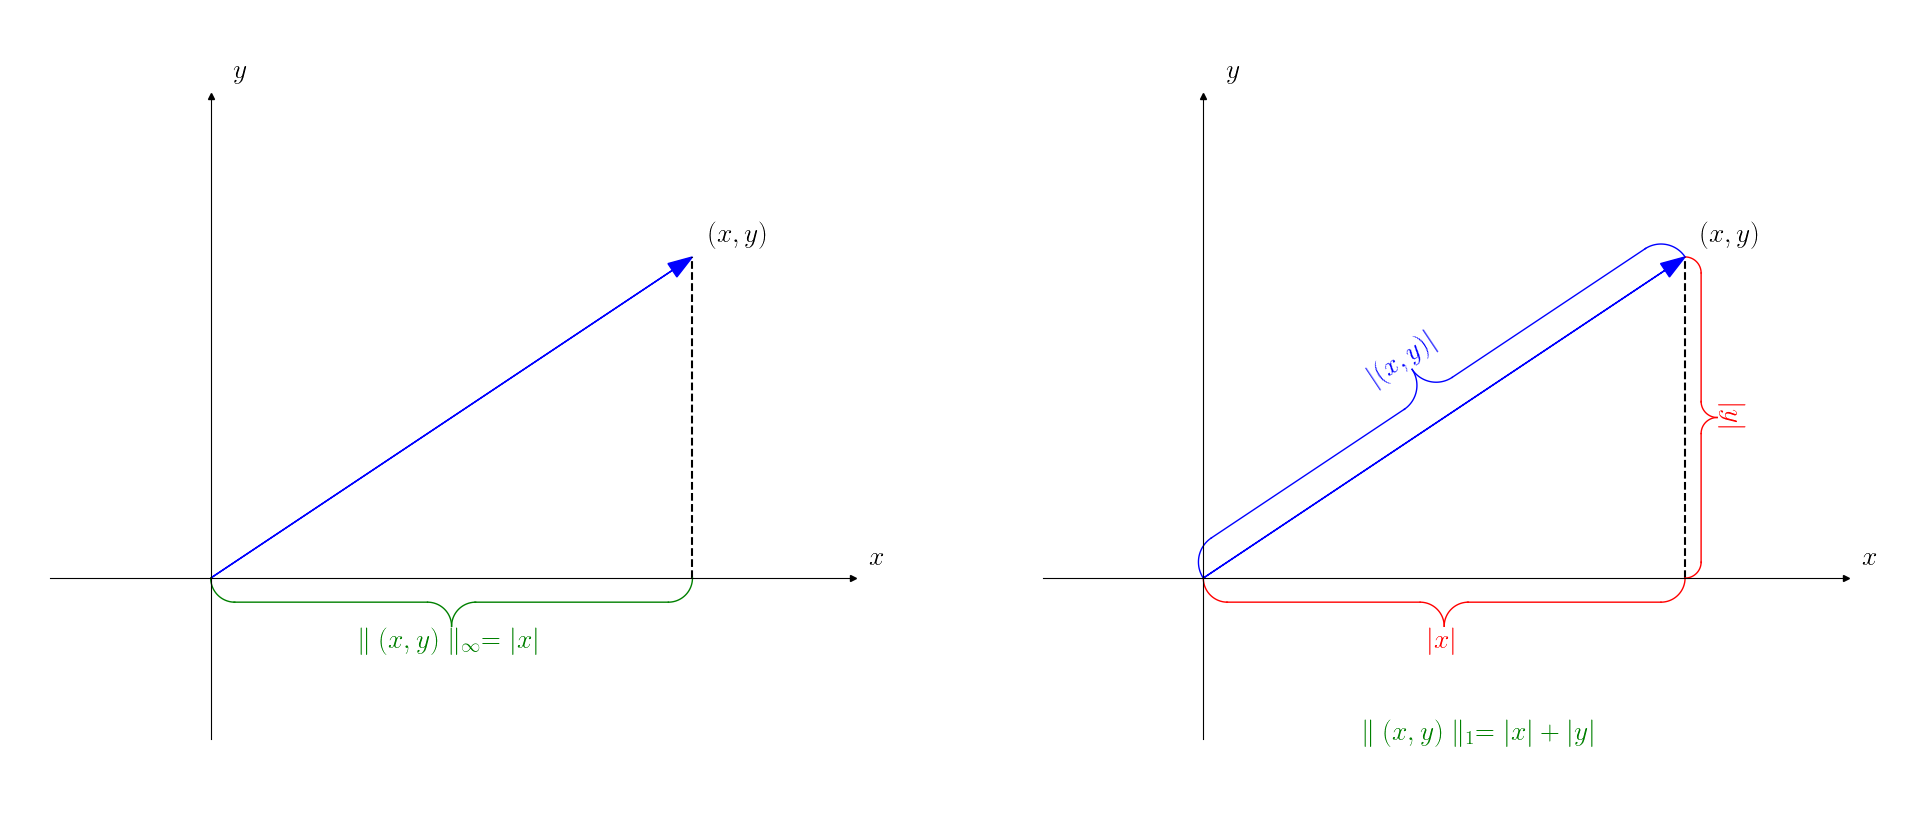
\includegraphics[width=\linewidth]{spazi_metrici_e_normati/pag126}
		\label{fig:pag126}
	\end{center}
	\begin{gather*}
		\parallel \overline{x} \parallel_p = \left( \sum_{i=1}^{n} |x_i|^p \right)^{\frac{1}{p}} \quad p \geq 1
		\\
		\parallel \overline{x} \parallel_\infty = \lim_{p \rightarrow +\infty} \parallel \overline{x} \parallel_p
	\end{gather*}
	$(\mathbb{R}^n, \parallel \cdot \parallel_p)$ è spazio normato

	\item $C^0 \left( [0,1] \right)$
	\begin{align*}
		&\parallel f \parallel_\infty = \sup_{x \in [0,1]} |f(x)| (=\max_{x \in [0,1]} |f(x)|)
		\\
		&\parallel f \parallel_1 = \int_{0}^{1} |f(x)| \ \mathrm{d}x
		\\
		&\parallel f \parallel_p = \left( \int_{0}^{1} |f(x)|^p \ \mathrm{d}x \right)^{\frac{1}{p}} \qquad p \geq 1
	\end{align*}

sono tute norme su $C^0 ([0,1])$
\end{itemize}
\end{exbar}


\begin{exbar}
\begin{example}
	Facciamo vedere che $\parallel \cdot \parallel_\infty$ su $C^0 ([0,1])$ è una norma
	\begin{enumerate}
		\item $\parallel f \parallel_\infty \geq 0 \qquad$ (banale)
		
		$\parallel f \parallel_\infty =  0 \iff f(x) = 0 \qquad \forall \ x \in [0, 1]$
		
		$\parallel f \parallel_\infty =  0 \iff \sup_{x \in [0,1]} |f(x)| = 0$
		
		$\iff 0 \leq |f(x)| \leq 0 \quad \forall \ x \in [0,1] \iff f(x) = 0 \qquad \forall \ x \in [0,1]$
		
		\item $\parallel \lambda f \parallel_\infty = |\lambda| \parallel f \parallel_\infty \qquad \forall \lambda \in \mathbb{R}$ e $\forall f \in C^0 ([0,1])$
		
		$\parallel \lambda f \parallel_\infty = \sup_{x \in[0,1]} |\lambda f(x)| = \sup_{x\in[0,1]} |\lambda| \ |f(x)| = |\lambda| \sup_{x\in[0,1]} |f(x)| = |\lambda| \parallel f \parallel_\infty$
		
		\item $\parallel f+g \parallel_\infty \leq \parallel f \parallel_\infty + \parallel g \parallel_\infty \qquad \forall f,g \in C^0 ([0,1])$
		
		$\parallel f+g \parallel_\infty = \sup_{x\in[0,1]} |f(x) + g(x)|$
		
		$|f(x) + g(x)| \distr |f(x)| + |g(x)| \leq \sup_{y\in[0,1]} |f(y)| + \sup_{y\in[0,1]} |g(y)| =  \parallel f \parallel_\infty + \parallel g \parallel_\infty \qquad \forall \ x \in [0,1]$
		
		$\parallel f+g \parallel_\infty = \sup_{x\in[0,1]} |f(x) + g(x)| \leq \parallel f \parallel_\infty + \parallel g \parallel_\infty$\\
	\end{enumerate}
\end{example}
\end{exbar}
	

\begin{exbar}
\begin{example}
		Facciamo vedere che $\parallel f\parallel_1 = \int_{0}^{1} |f(x)| \ \mathrm{d}x$
		
		è una norma
	\begin{enumerate}
		\item $\parallel f \parallel_1 \geq 0 \qquad \forall f \in C^0 ([0,1]) \text{ banale}$
		
		Dimostriamo che $\parallel f \parallel_1 = 0 \iff f(x) = 0 \qquad \forall \ x \in [0,1]$
		
		$\Leftarrow) f(x) = 0 \qquad \forall \ x \in[0,1]$
		
		$\parallel f \parallel_1 = \int_{0}^{1} 0 \ \mathrm{d}x = 0$
		
		$\Rightarrow)$ Sia $\parallel f \parallel_1 = 0$ e dimostriamo che $f(x) = 0 \qquad \forall \ x \in [0,1]$
		
		$\int_{0}^{1} |f(x)| \ \mathrm{d}x = 0$
		
		Se $\exists \ x_0 \in [0,1]$ tale che $|f(x_0)| \neq 0$ allora $\exists$ un intorno $U$ di $x_0 $ tale che $|f(x)| \geq \frac{|f(x_0)|}{2}$ $\qquad \forall x \in U \cap [0,1]$ 
		
		\begin{itemize}
			\item $U = \ ]x_0 - \delta, x_0 + \delta[ \ \subseteq [0,1]$
	
			\item $x_0=0$
			
			$U= \ ]0 - \delta, 0 + \delta[$
			
			$U \cap [0,1] = [0, \delta[$
			
			\item $x_1 = 1$
			 $U= \ ]1 - \delta, 1 + \delta[$
			 
			$U \cap [0, 1] = \ ]1 - \delta, 1]$
		\end{itemize}
		
		cioè in ogni caso $U \cap [0,1]$ è un intervallo di ampiezza almeno $\frac{\delta}{2}>0$
		
		\begin{equation*}
			\parallel f\parallel_1 = \int_{0}^{1} |f(x)| \ \mathrm{d}x \geq \int_{U \cap [0,1]} |f(x)| \ \mathrm{d}x \geq \int_{U \cap [0,1]} \frac{|f(x_0)|}{2} \ \mathrm{d}x \geq \frac{\delta}{4} |f(x_0)| > 0
		\end{equation*}
		
		il che è assurdo, perché $\parallel f\parallel_1 = 0$
		
		\item $\parallel \lambda f \parallel_1 = \int_{0}^{1} |\lambda f(x)| \ \mathrm{d}x = |\lambda| \int_{0}^{1} |f(x)| \ \mathrm{d}x = |\lambda| \parallel f \parallel_1 \qquad \lambda \in \mathbb{R}$
		
		\item $f,g \in C^0 ([0,1])$
		
		$\parallel f+g \parallel_1 = \int_{0}^{1} |f(x) + g(x)| \ \mathrm{d}x \leq \int_{0}^{1} (|f(x)| + |g(x)|) \ \mathrm{d}x = \parallel f \parallel_1 + \parallel g \parallel_1$
		
		$\Rightarrow$ vale la disuguaglianza triangolare
	\end{enumerate}
\end{example}
\end{exbar}


\begin{attbar}
	Dato uno spazio normato $(X, \parallel \cdot \parallel)$ posso definire la distanza tra due vettori $x,y \in X$ come $d(x,y)= \parallel x-y \parallel$, lunghezza del vettore $x-y$
	\begin{center}
		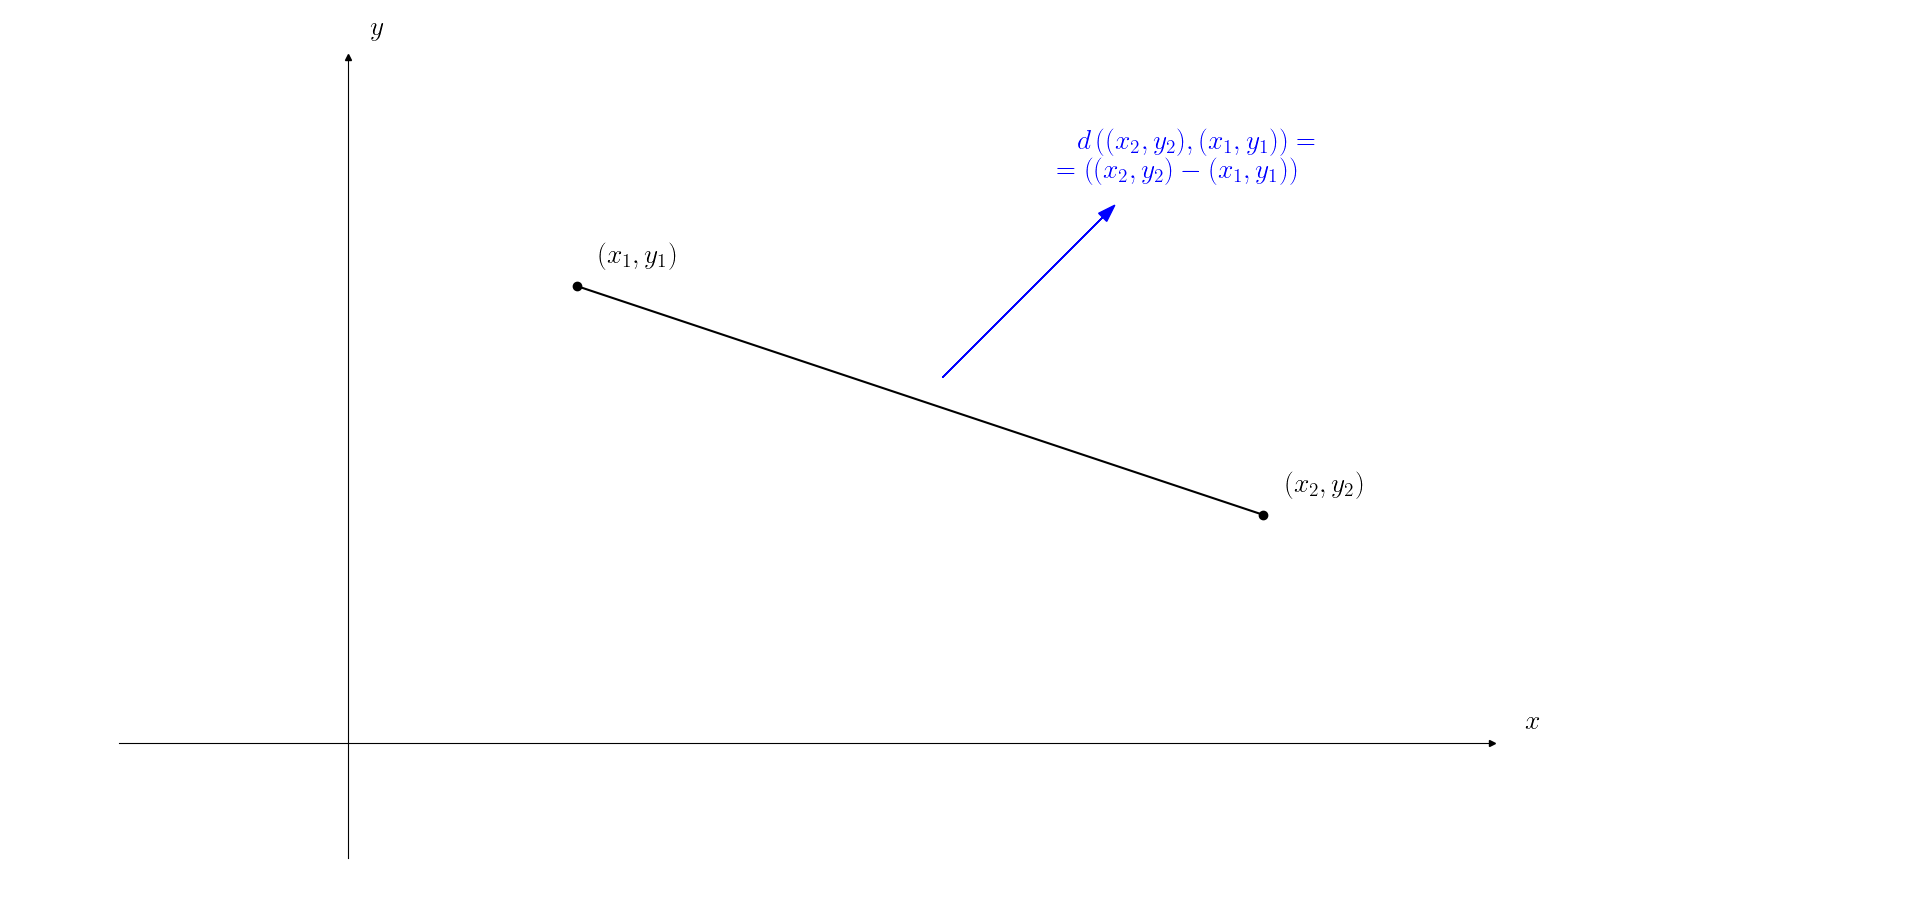
\includegraphics[width=0.75\linewidth]{spazi_metrici_e_normati/pag131}
		\label{fig:pag131}
	\end{center}
\end{attbar}


\begin{definition}
	$X$ insieme non vuoto. Una distanza o metrica su $X$ è una funzione $d:X \times X \rightarrow \mathbb{R}$ tale che
	\begin{enumerate}
		\item $d(x,y) \geq 0 \qquad \forall \ x,y \in X $ e $d(x,y) = 0 \iff x = y$
		\item $d(x,y) = d(y,x)$ (proprietà simmetrica)
		\item Disuguaglianza triangolare $d(x,y) \leq d(x,z) + d(z,y) \qquad \forall \ x,y,z \in X$
	\end{enumerate}
	
	La coppia $(X,d)$ si dice \textbf{spazio metrico}.
\end{definition}



$(X, \parallel \cdot \parallel)$ normato

$d(x,y)=\parallel x-y \parallel$ è metrica, allora
\begin{enumerate}
	\item $d(x,y)\geq 0$ banalmente 
	$d(x,y) = \parallel x-y \parallel = 0 \iff x-y = 0 \iff x = y$
	\item $d(x,y) = \parallel x-y \parallel = \parallel y-x \parallel = d(y,x)$
	\item $d(x,y) = \parallel x-y \parallel = \parallel (x-z) + (z-y) \parallel \leq \parallel x-z \parallel + \parallel z-y \parallel = d(x,z) + d(y,z)$
\end{enumerate}

Dato uno spazio vettoriale $X$ e $d$ metrica su $X$, esiste una norma $\parallel \cdot \parallel$ su $X$ tale che $d(x,y) = \parallel x-y \parallel$?

No, esistono metriche dentro lo spazio vettoriale che non derivano da una norma.


\begin{exbar}
\begin{example}
	$\mathbb{R}, \quad 0 < p < 1 , \quad d(x,y) = |x-y|^p$. 
	
	Allora $d$ è una metrica, che non deriva da una norma.
	
	Se esistesse una norma $\parallel \cdot \parallel$ su $\mathbb{R}$ tale che $d(x,y) = \parallel x-y \parallel$, allora, fissato $\lambda \in \mathbb{R}$,
	\begin{gather*}
		d(\lambda x, \lambda y) = \parallel \underbrace{\lambda x - \lambda y}_{\lambda (x - y)} \parallel \uppercomment{=} {\text{seconda}} {\text{proprietà di }\parallel \cdot \parallel} |\lambda| \parallel x-y \parallel = |\lambda | \ d(x,y)
		\\
		d(\lambda x, \lambda y) = |\lambda x - \lambda y|^p = |\lambda|^p |x-y|^p = |\lambda|^p d(x,y) \neq |\lambda| \ d(x,y) \text{ se } |\lambda \neq 1,0|
	\end{gather*}
	
	Facciamo vedere che $d(x,y) = |x-y|^p$ è una distanza, $0 < p < 1$
	\begin{enumerate}
		\item $d(x,y) \geq 0$ banale
		
		$d(x,y) = 0 \iff |x-y|^p = 0 \iff |x-y| = 0 \iff x = y$
		
		\item $d(x,y) = d(y,x)$ banale
		
		\item Disuguaglianza triangolare
		
		Dobbiamo dimostrare che $\forall \ x,y,z \in \mathbb{R}$ vale
		\begin{gather*}
			d(x,y) \leq d(x,z) + d(z,y)
			\\
			|x-y|^p \leq |x-z|^p + |z-y|^p
			\\
			|x-y|^p \distr (|x-z| + |y-z|)^p
		\end{gather*} 
	
		Se dimostro che $( \underbrace{|x-z|}_{= a} + \underbrace{|y-z|}_{=b})^p \leq |x-z|^p + |z-y|^p$, sono a posto $\forall \ x,y,z \in \mathbb{R}$ con $0<p<1$.
		
		Devo dunque dimostrare che $(a+b)^p \leq a^p + b^p \qquad \forall \ a,b \in \mathbb{R}^{\geq 0}$.
		
		Se $a=0$ o $b=0$, banale
		
		Siano $a,b \neq 0$
		\begin{gather*}
		(a + b)^p \leq a^p + b^p \qquad /.\frac{1}{b^p}
		\\
		\iff \frac{(a+b)^p}{b^p} \leq \frac{a^p}{b^p} + 1 \iff \left( \frac{a+b}{b} \right)^p \leq \left( \frac{a}{b} \right)^p + 1 \iff \left( \frac{a}{b} + 1 \right)^p \leq \left( \frac{a}{b} \right)^p + 1 \qquad \forall \ a,b > 0
		\end{gather*}
		
		Posto $\lambda = \frac{a}{b}>0$
		\begin{gather*}
		\left( \frac{a}{b} + 1 \right)^p \leq \left( \frac{a}{b} \right)^p + 1 \qquad \forall \ a,b>0 \iff (\lambda + 1)^p \leq \lambda^p + 1 \qquad \forall \ \lambda > 0
		\\
		(\lambda + 1)^p - \lambda^p \leq 1
		\\
		f(\lambda) = (\lambda + 1)^p -\lambda^p \qquad f:\mathbb{R}^{\geq 0} \rightarrow \mathbb{R}
		\\
		f(\lambda) \leq 1 = f(0)
		\\
		f'(\lambda) 
		\lowercomment{=} {\myarrow[270]} {\lambda \neq 0} p \ (\lambda + 1)^{p - 1} - p \ \lambda^{p - 1} 
		= p \ [(\lambda + 1)^{p - 1} - \lambda^{p - 1}] 
		= p \ \lambda^{p - 1} \left[ \left( \frac{\lambda + 1}{\lambda} \right)^{p-1} - 1 \right] 
		\\
		=  p \ \lambda^{p - 1} \left[ \underbrace{ \left(  1 + \frac{1}{\lambda} \right) ^{\overbrace{p - 1}^{<0}} }_{<1} - 1 \right] < 0 \qquad \forall \ \lambda > 0
 		\end{gather*}
		
		$f$ è decrescente e quindi $\forall \ \lambda > 0 \Rightarrow f(\lambda) \leq f(0)$, come si voleva.
	\end{enumerate}
\end{example}
\end{exbar}


\subsection{Topologia}

$(x,d)$ spazio metrico.

\begin{definition}
	
\end{definition}
	Sia $x \in X, r >0$, allora $B_r(x) = \{ y \in X | d(x,y) < r \}$ si dice \textbf{palla (aperta)} di centro $x$ e raggio $r$.

	
\begin{exbar}
	\begin{gather*}
		(\mathbb{R}^2, | \cdot |), \qquad \mathbb{R}^2 \text{ con norma euclidea}
		\\
		B_r (0,0), \qquad r > 0
		\\
		B_r (0,0) 
		= \{ (x,y) \in \mathbb{R}^2 \big| d((x,y), (0,0)) < r \} 
		= \{ (x,y) \in \mathbb{R}^2 \big| |(x,y)-(0,0)| < r \} =
		\\ 
		= \{ (x,y) \in \mathbb{R}^2 \big| \sqrt{x^2+y^2} < r\}
	\end{gather*}
	\begin{center}
		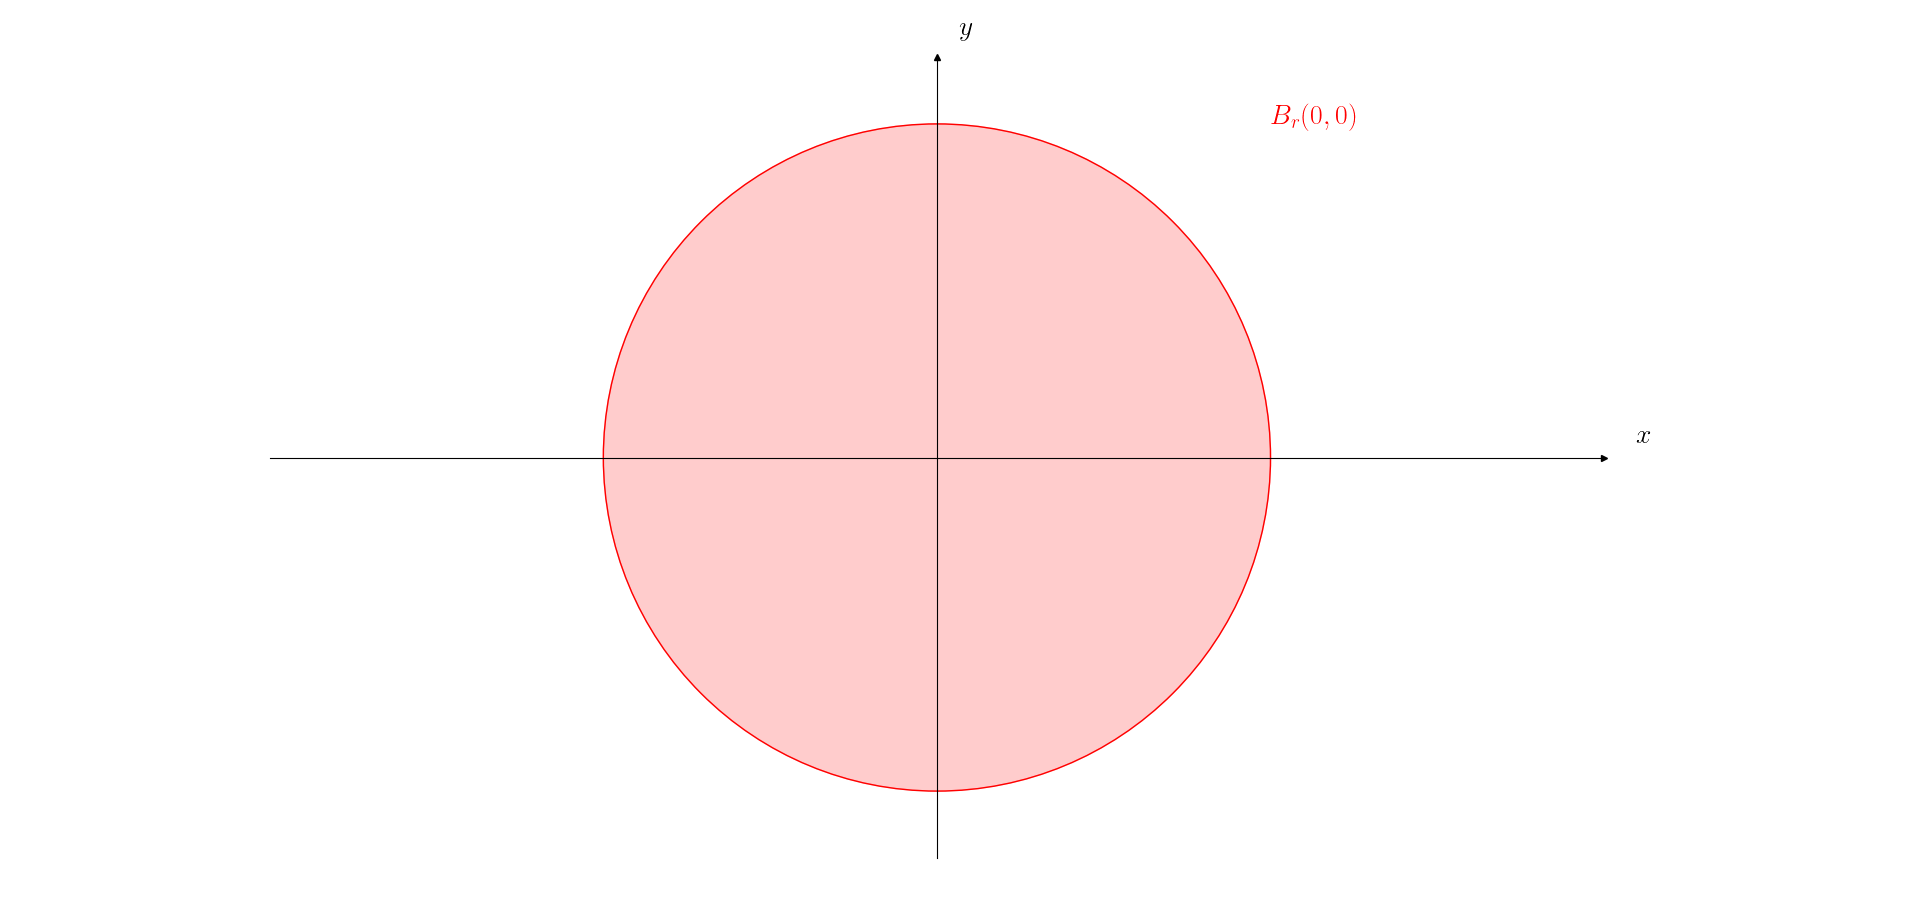
\includegraphics[width=0.75\linewidth]{spazi_metrici_e_normati/pag137circle}
		\label{fig:pag137circle}
	\end{center}
	
	\begin{gather*}
	 	(\mathbb{R}^2, \parallel \cdot \parallel_\infty)
	 	\\
		\parallel (x,y) \parallel_\infty = \max \{|x|,|y|\} 
		\\
		B_r^\infty (0,0) 
		= \{ (x,y) \in \mathbb{R}^2 \big| \parallel(x,y) - (0,0) \parallel_\infty < r \} 
		= \{ (x,y) \in \mathbb{R}^2 \big| \max \{|x|,|y| \} < r \} =
		\\
		= \{ (x,y) \in \mathbb{R}^2 \big| |x|,|y| < r\}
	\end{gather*}
	\begin{center}
		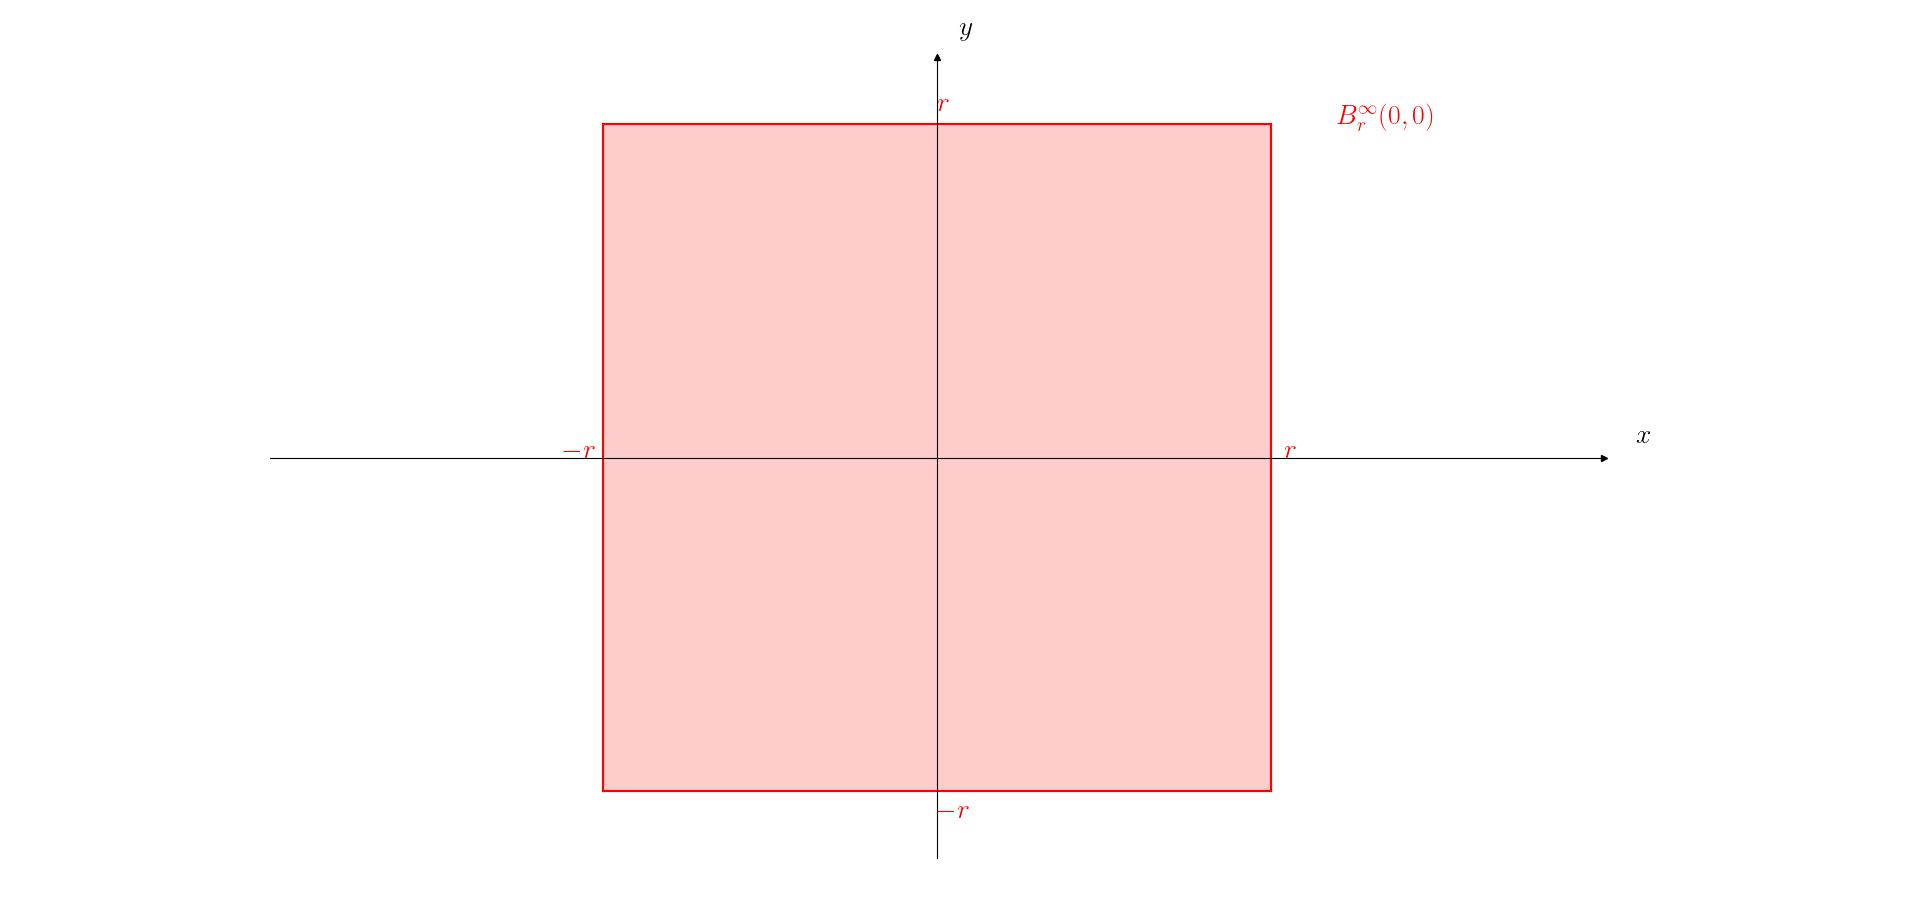
\includegraphics[width=0.75\linewidth]{spazi_metrici_e_normati/pag137square}
		\label{fig:pag137square}
	\end{center}
	
	\begin{gather*}
		(\mathbb{R}^2, \parallel \cdot \parallel_1)
		\qquad
		\parallel (x,y) \parallel_1 = |x| + |y| 
		\\
		B_r^1 (0,0) = \{(x,y) \in \mathbb{R}^2 \big| \parallel (x,y) - (0,0) \parallel_1 < r \} 
		= \{(x,y) \in \mathbb{R}^2 \big| |x| + |y| < r \}
	\end{gather*}
	\begin{center}
		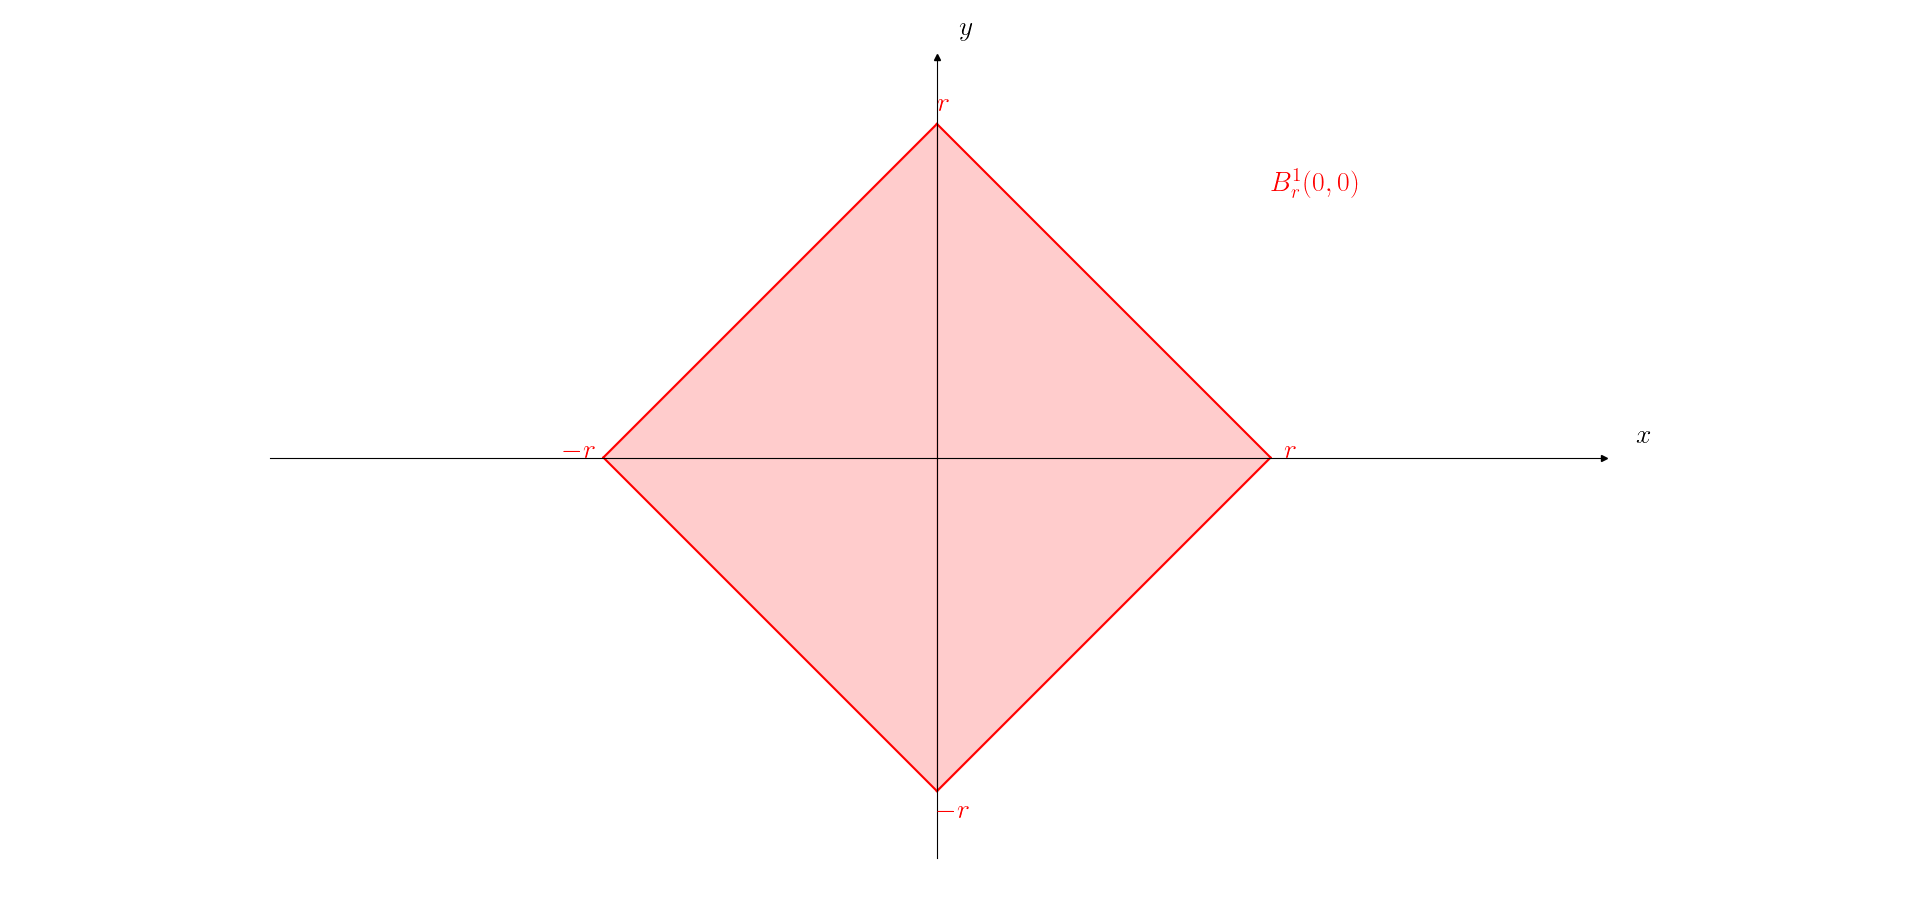
\includegraphics[width=0.75\linewidth]{spazi_metrici_e_normati/pag138rhombus}
		\label{fig:pag138rhombus}
	\end{center}

	\begin{gather*}
		(C^\circ([0,1]), \parallel \cdot \parallel_\infty) \qquad
		d(f,g) = \parallel f-g \parallel_\infty
		\\
		f \in C^0 (), \qquad r>0
		\\
		B_r^\infty(f) = \{ g \in C^0 ([0,1]) \big| \parallel f-g \parallel_\infty < r \} = \{ g \in C^0 ([0,1]) \big| \undercomment{\sup_{x \in [0,1]} |f(x) - g(x)|} {f(x) - r < g(x) < f(x) + r} {} < r \} 
	\end{gather*}		
	\begin{center}
		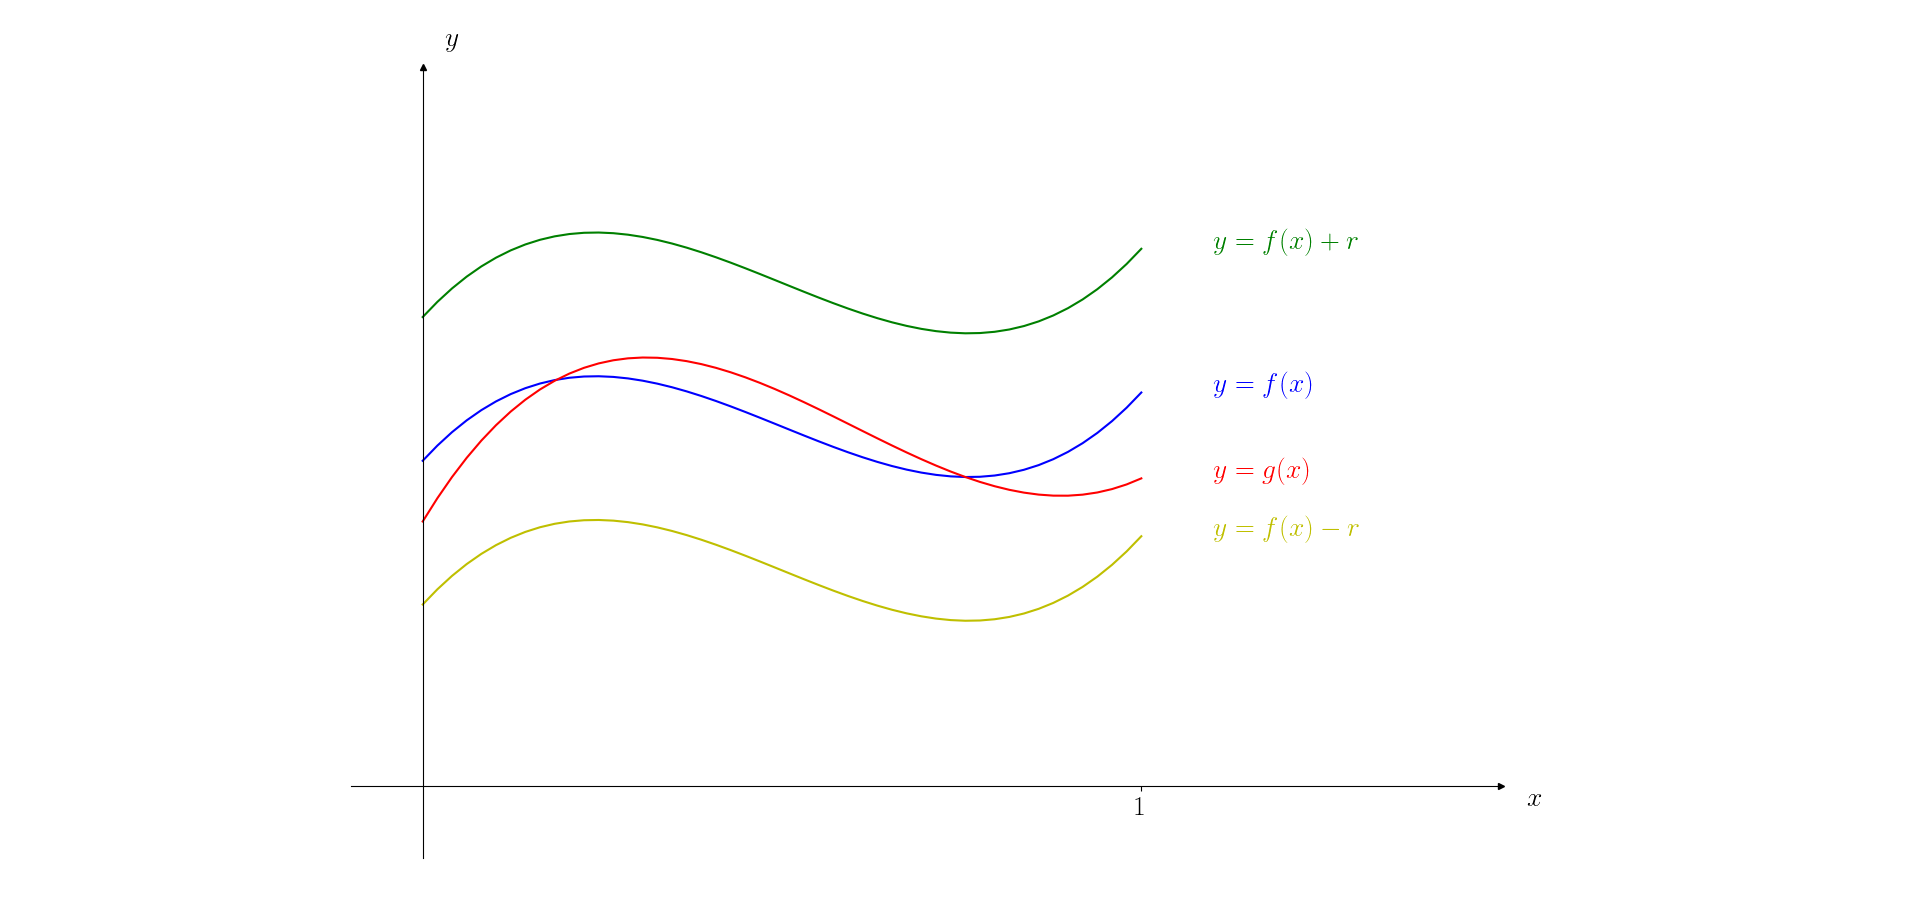
\includegraphics[width=0.75\linewidth]{spazi_metrici_e_normati/pag138curve}
		\label{fig:pag138curve}
	\end{center}
	
	$$f(x)=0 \qquad \forall \ x \in [0,1]$$
	\begin{center}
		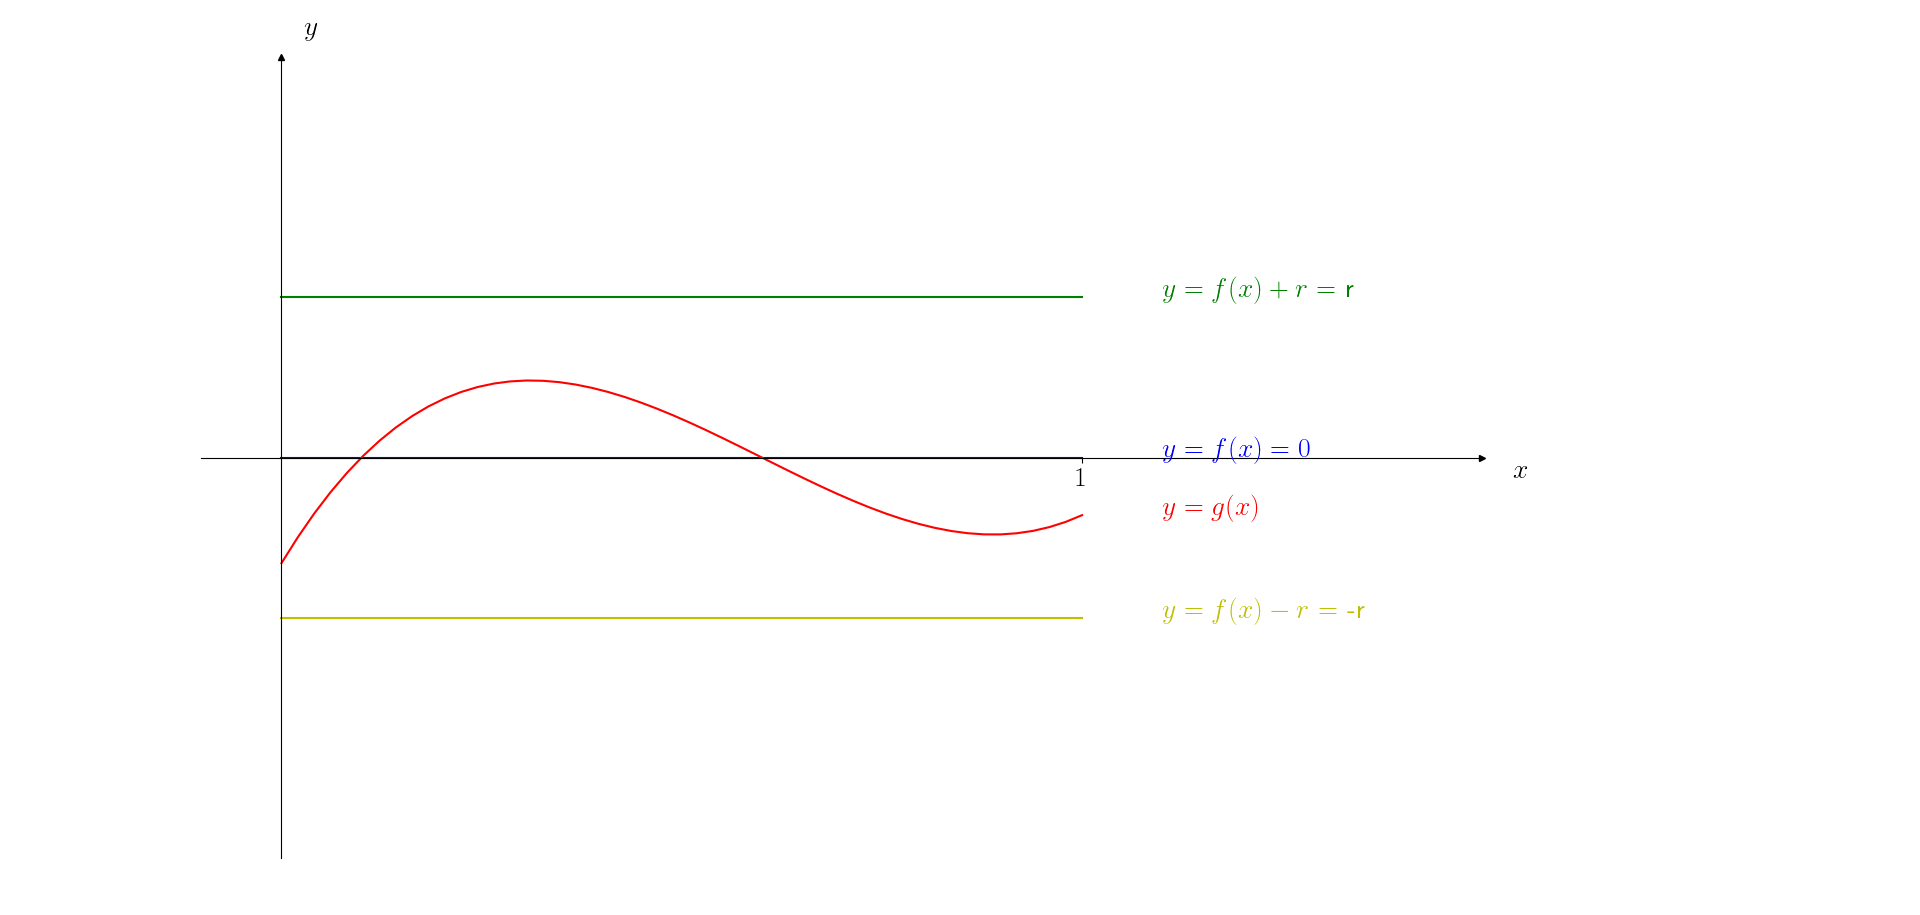
\includegraphics[width=0.65\linewidth]{spazi_metrici_e_normati/pag139curve}
		\label{fig:pag139curve}
	\end{center}
	
	\begin{gather*}
		C^0 ([0,1]), \parallel \cdot \parallel_1
		\\
		\parallel f \parallel_1 = \int_{0}^{1} |f(x)| \ \mathrm{d}x 
		\\
		B_r^1 = \{ g \in C^0 ([0,1]) \big| \parallel f-g \parallel_1 < r \} = \{g \in C^0 ([0,1]) \bigg| \int_{0}^{1} |f(x) - g(x)| \ \mathrm{d}x < r \}
		\\
		f(x) = 0 \qquad \forall \ x \in [0,1]
		\\
		B_r^1(0) = \{ g \in C^0 ([0,1]) \bigg| \int_{0}^{1} |g(x)| \ \mathrm{d}x < r \}
	\end{gather*}
	\begin{center}
		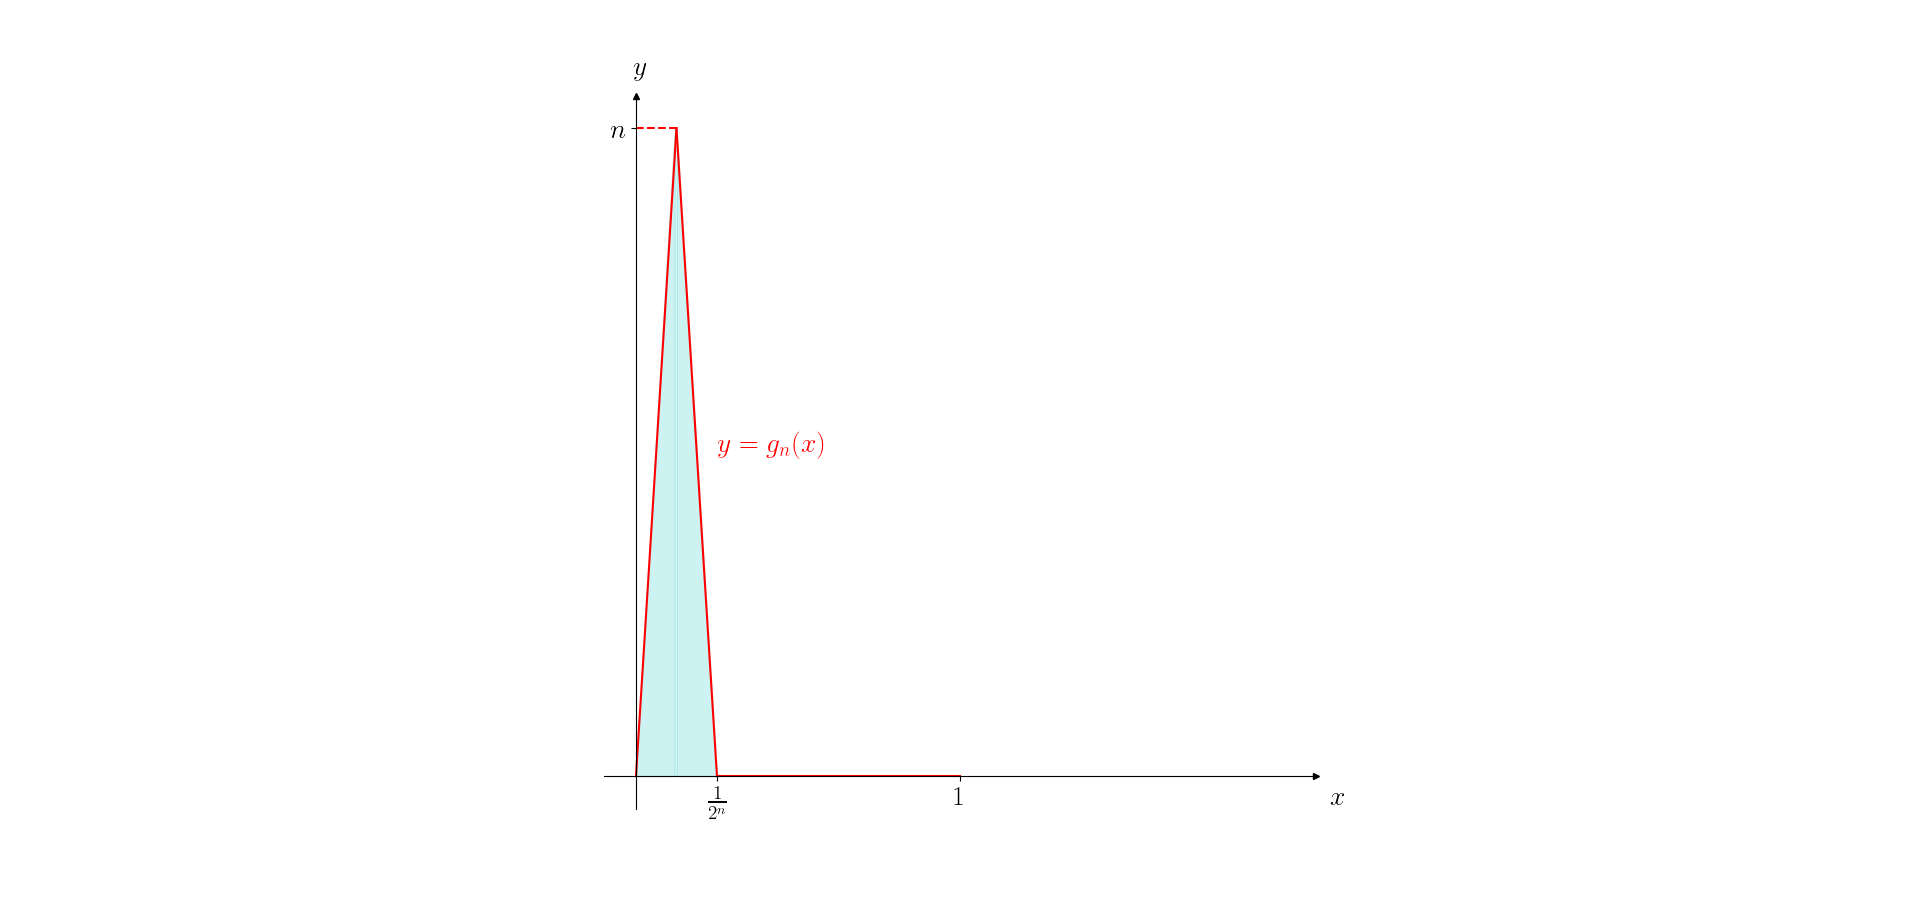
\includegraphics[width=0.85\linewidth]{spazi_metrici_e_normati/pag139triangolo}
	\end{center}

	$\int_{0}^{1} |g_n(x)| \ \mathrm{d}x =$ area del triangolo $ = \frac{1}{2} \frac{1}{2^n} n = \lowercomment{\frac{n}{2^{n+1}}} {\myarrow[270]} {0 \text{ per } n \rightarrow + \infty}$

	Fissato $r > 0$, trovo $n$ tale che $\int_{0}^{1} |g_n(x)| \ \mathrm{d}x < r$	
\end{exbar}


\begin{definition}
	$x \in X$. Un \textbf{intorno di $x$} è un qualsiasi sottoinsieme $A \subseteq X$ che contiene una palla aperta centrata in $x$, cioè per cui $\exists \ r > 0 \big| B_r(x) \subseteq A$
\end{definition}


\begin{definition}
	$A \subseteq X$ si dice \textbf{aperto} se è intorno di ogni suo punto, cioè se $\forall \ x \in A \quad \exists r > 0 \ \big| \ B_r(x) \subseteq A$.
	
	$A$ si dice \textbf{chiuso} se $A^c = X \backslash A$ è aperto.
\end{definition}


\begin{exbar}
\begin{example}
	$(x,d)$ spazio metrico, $x \in X, r>0$, $B_r(x)$ è un aperto.
	
	Devo far vedere che $\forall \ y \in B_r(x) \ \exists \ \overline{r} > 0 \ \big| \; B_{\overline{r}}(y) \subseteq B_r(x)$
	
	$\overline{r} = r - d(x,y) > 0$ perché $d(x,y) < r$ e dimostriamo che, se $z \in B_{\overline{r}} (y)$, allora $z\in B_r(x)$, cioè, se $d(y,z)< \overline{r}$, allora $d(x,z)<r$
	
	$d(x,z) \distr  d(x,y) + d(y,z) < d(x,y) + \overline{r} = d(x,y) + (r-d(x,y)) = r$	
	\begin{center}
		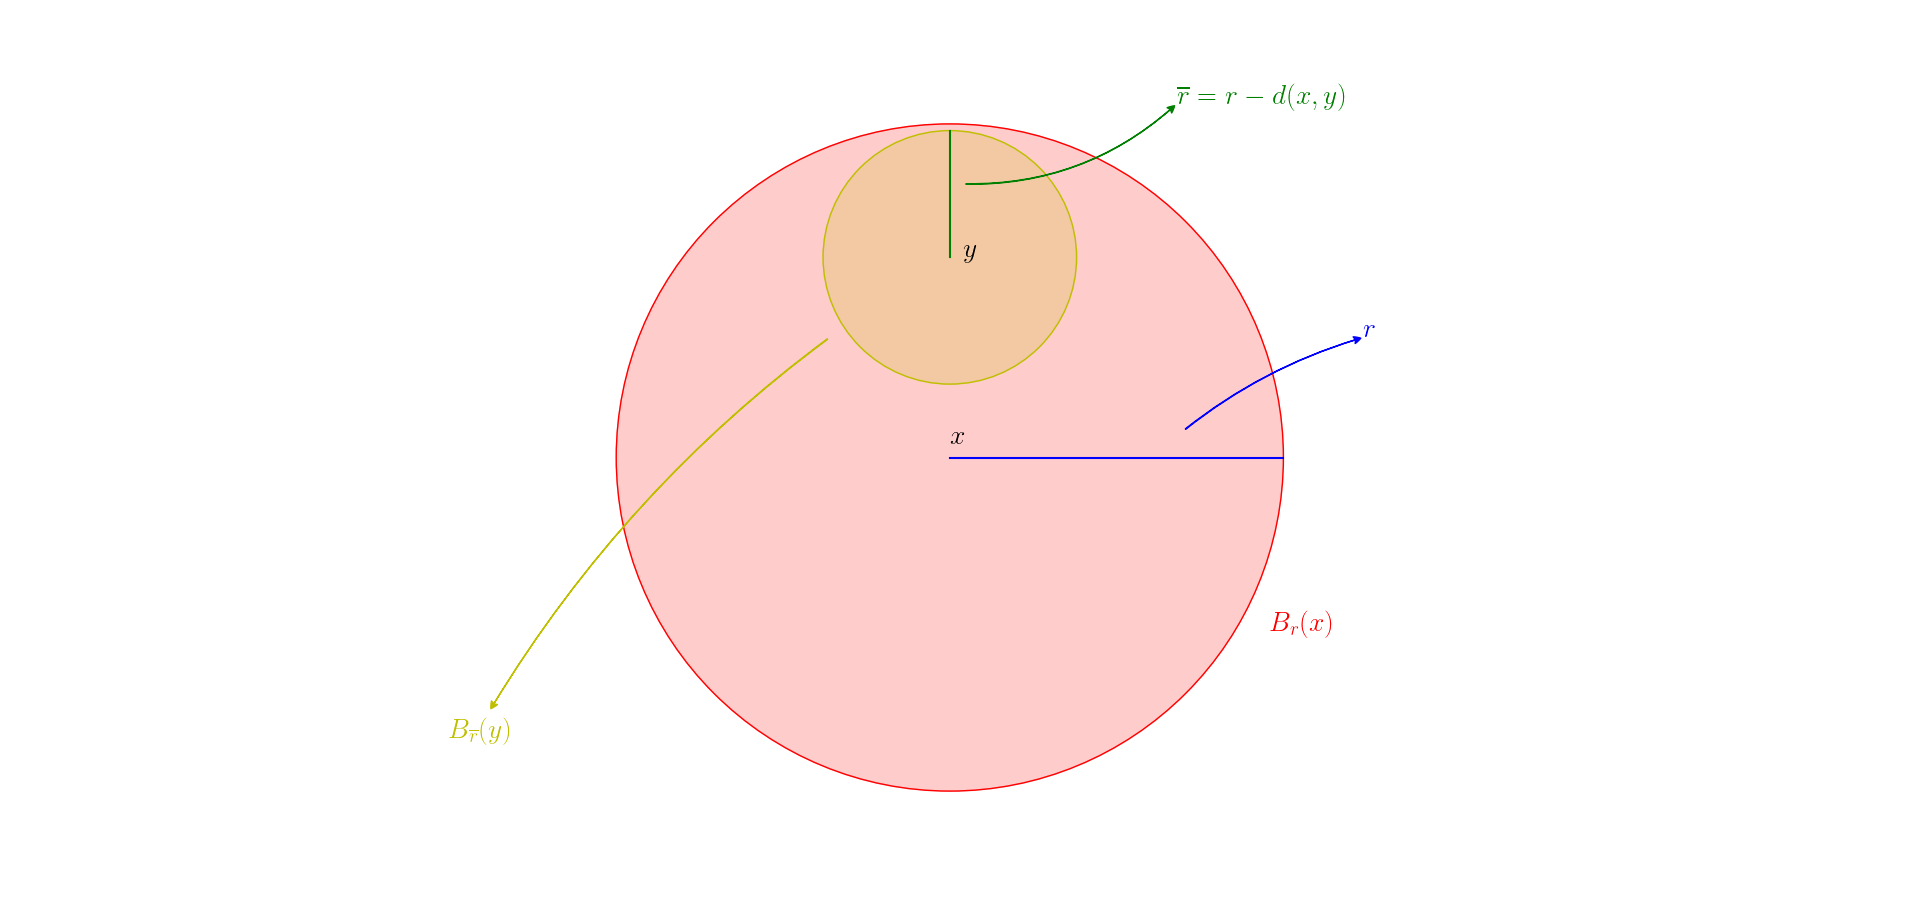
\includegraphics[width=0.75\linewidth]{spazi_metrici_e_normati/pag141}
		\label{fig:pag141}
	\end{center}
\end{example}
\end{exbar}


\begin{exbar}
	$(\mathbb{R}^2, \parallel \cdot \parallel_\infty)$
	\begin{center}
		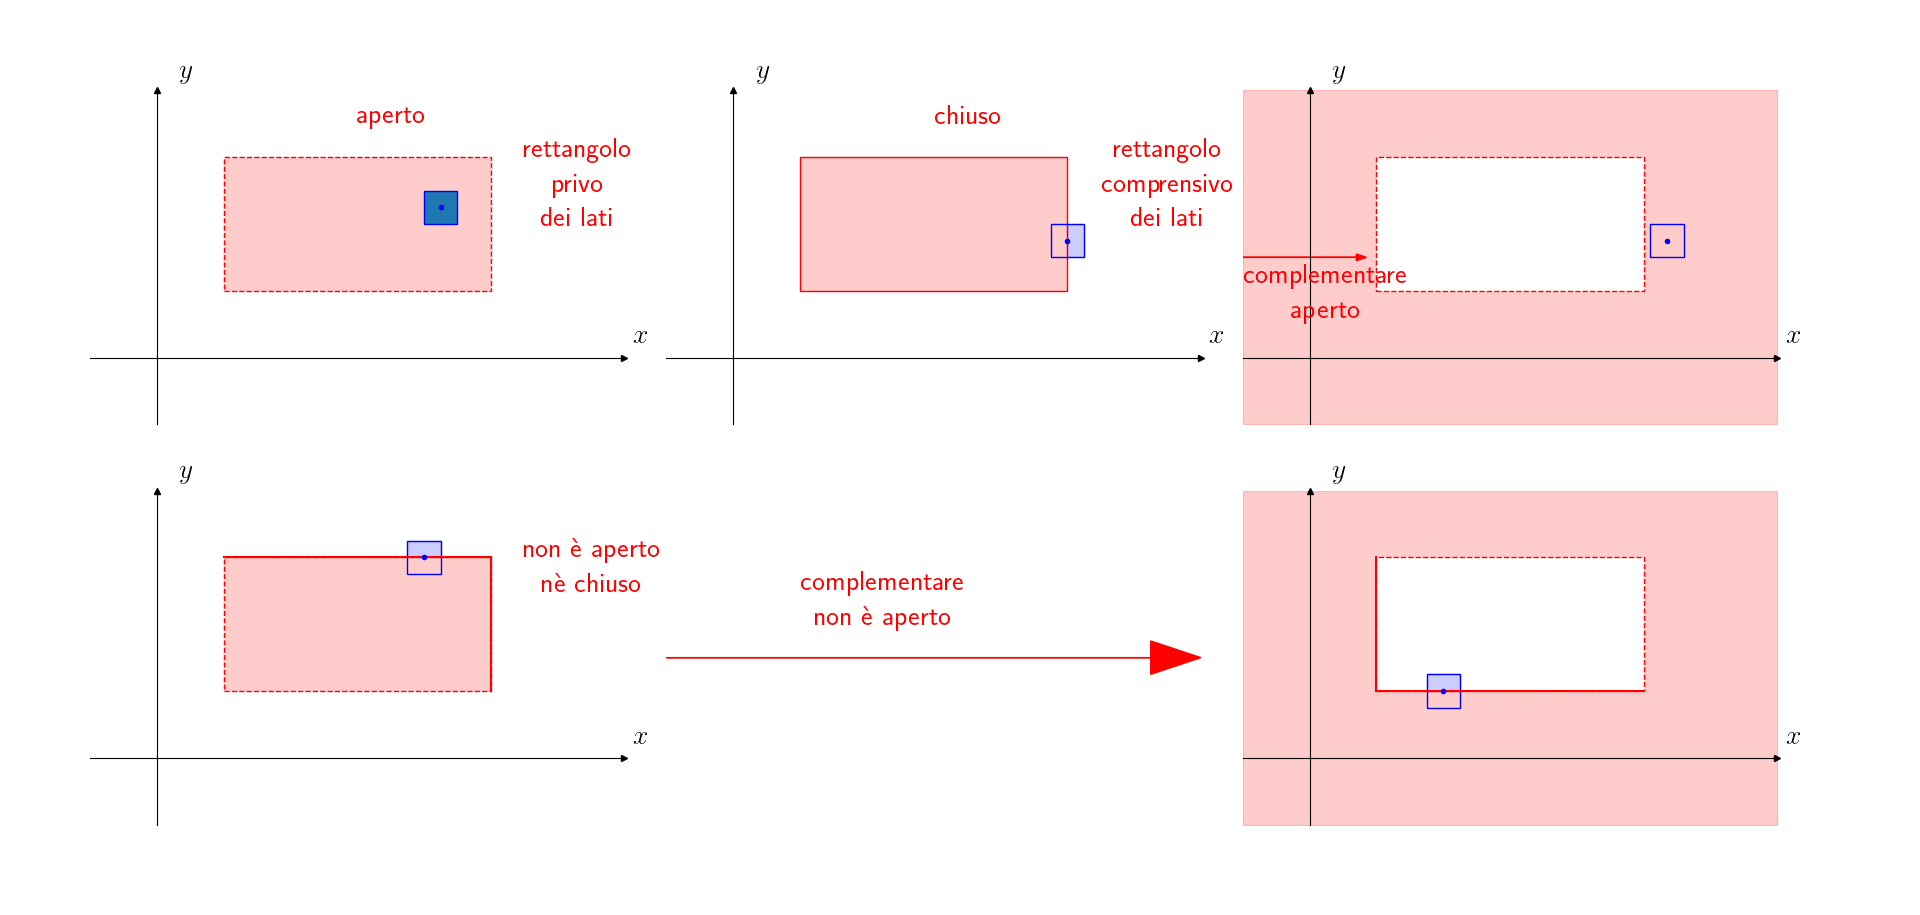
\includegraphics[width=\linewidth]{spazi_metrici_e_normati/pag141-142}
		\label{fig:pag141-142}
	\end{center}
\end{exbar}


\textbf{Osservazione:} 
	$(X,d)$ spazio metrico, $X$ è aperto banalmente (se $x \in X, B_r(x) \subseteq X \ \forall \ r > 0$) e quindi $\emptyset = X^c = X \backslash X$ è chiuso. 
	
	D'altra parte $\emptyset $ è aperto perché l'implicazione $x \in \emptyset \Rightarrow  \ \exists \ r > 0 \ \big| \ B_r(x) \subseteq \emptyset$ è vera perché $x \in \emptyset$  è falsa $\Rightarrow \emptyset^c = X \backslash \emptyset = X$ è chiuso. 
	
	\begin{attbar}
		$\emptyset, X$ sono sia aperti che chiusi.
	\end{attbar}


\begin{theorem}
	
	$(X,d)$ spazio metrico
	\begin{enumerate}
		\item $A_1, A_2 \subseteq X$ aperti $\Rightarrow A_1 \cap A_2$ è un aperto.
		 
		\item $\{A_i\}_{i \in I}$ è una famiglia di aperti, allora $\bigcup_{i \in I} A_i$ è un aperto.
		
		\item Se $C_1, C_2 \subseteq X$ sono chiusi, allora $C_1 \cup C_2$ è chiuso.
		
		\item $\{C_i\}_{i\in I}$ è famiglia di chiusi, allora $\bigcap_{i \in I} C_i$ è un chiuso.
	\end{enumerate}
\end{theorem}


\textbf{Osservazione:} 
In generale se $\{ A_i \}_{i \in I}$ è una famiglia infinita di aperti, allora $\bigcap_{i \in I} A_i$ non è un aperto e, se $\{ C_i \}_{i \in I}$ è una famiglia infinita di chiusi, allora $\bigcup_{i \in I} C_i$ non è chiuso. Facciamo un esempio.

$A_k= \ \bigg]-\frac{1}{k}, \frac{1}{k} \bigg[ \qquad k \geq 1, k \in \mathbb{N}$ sono tutti aperti di $\mathbb{R}$, allora $\bigcap_{k=1}^\infty A_k = \bigcap_{k=1}^\infty \ \bigg] -\frac{1}{k}, \frac{1}{k} \bigg[ \ = \{ 0 \}$, che è un chiuso.

$C_k = \left[ \frac{1}{k}, 1-\frac{1}{k} \right], \qquad k \geq 2, k \in \mathbb{N}$ sono tutti chiusi 

\bigg( $C_k^c = \ \bigg] -\infty, \frac{1}{k} \bigg[ \ \cup \ \bigg] 1-\frac{1}{k}, +\infty \bigg[$, unione di due intervalli aperti \bigg)

$\bigcup_{k=2}^\infty C_k = \bigcup_{k=2}^\infty \left[ \frac{1}{k}, 1-\frac{1}{k} \right] = \ ]0,1[$

Infatti, se $x \in \bigcup_{k=1}^\infty \left[ \frac{1}{k}, 1-\frac{1}{k} \right]$, allora $\exists \ \overline{k} \geq 2 \ \big| \ \left[\frac{1}{k}, 1-\frac{1}{k}\right]$, cioè $0 < \frac{1}{k} \leq x \leq 1- \frac{1}{k} < 1$

$\Rightarrow 0 < x < 1 \Rightarrow x \in \ ]0,1[.$

D'altra parte, se $x \in \ ]0,1[$, esistono $k_1$ e $k_2 \ \big| \ \frac{1}{k_1} < x<1 - \frac{1}{k_2}$

$k=\max\{k_1, k_2\}$ 

\begin{gather*}
	\frac{1}{k} \leq \frac{1}{k_1} < x < 1 - \frac{1}{k_2} \leq 1 - \frac{1}{k}
	\\
	\Rightarrow x \in C_k = \left[ \frac{1}{k}, 1 - \frac{1}{k} \right]
	\\
	\Rightarrow x \in \bigcup_{k=2}^{\infty} C_k
\end{gather*}


\begin{definition}
	
	$(X,d)$ spazio metrico, $A \subseteq X, \ x \in A$. $x$ si dice \textbf{punto interno di A} se $\exists \ r > 0 \ \big| \ B_r(x) \subseteq A$. L'interno di $A$ è l'insieme dei punti interni di $A$ ed è indicato con \AA
\end{definition}


\begin{proposition}
	\label{pr: grande aperto}
	\AA \ è un insieme aperto ed è il più grande aperto, nel senso dell'inclusione, contenuto in $A$, cioè se $B \subseteq A$ è aperto, allora $B \subseteq \AA$
\end{proposition}

\begin{dembar}
	\textbf{Dimostrazione} della \textbf{Proposizione \ref{pr: grande aperto}} (Esercizio per casa)
\end{dembar}


\begin{exbar}
	\begin{gather*}
		A = \ ]0,1], \qquad \AA = \ ]0,1[
		\\
		A = \ ]0,1] \cup \{ 2 \}, \qquad \AA = \ ]0,1[
		\\
		A = \ ]0,1] \cup \left\{2 + \frac{1}{n} \ \bigg| \ n \geq 1, n \in \mathbb{N} \right\}, \qquad \AA = \ ]0,1[
	\end{gather*}
\end{exbar}


\begin{definition}
	$A \subseteq X, x \in X$ si dice \textbf{punto di chiusura} per $A$ se $B_r(x) \cap A \neq \emptyset \ \forall \ r > 0$, cioè ogni palla di centro $x$ interseca $A$. 
	
	La chiusura di $A$ è l'insieme di tutti i punti di chiusura di $A$ ed è denotata con $\overline{A}$.
\end{definition}


\begin{proposition}
	\label{pr: grande chiuso}
	$\overline{A} $ è un insieme chiuso ed è il più piccolo chiuso, nel senso dell'inclusione, contenente $A$, cioè, se $C \geq A$ è chiuso, allora $\overline{A} \subseteq C$
\end{proposition}


\begin{dembar}
	\textbf{Dimostrazione} della \textbf{Proposizione \ref{pr: grande chiuso}} (Esercizio per casa)
\end{dembar}


\begin{exbar}
	\begin{gather*}
		A = \ ]0,1], \qquad \lowercomment{\overline{A} = [0,1]} {0 \notin A, \text{ mentre se } x \in \AA \Rightarrow x \in A} {x \in A \Rightarrow x \in \overline{A} \text{ perché } x \in B_r(x) \cap A \ \forall r > 0}
		\\
		A = \ ]0,1] \cup \{ 2 \}, \qquad \overline{A} = [0,1] \cup \{ 2 \}
		\\
		A = \ ]0,1] \cup \left\{ 2 + \frac{1}{n} \ \bigg| \ n \geq 1, n \in \mathbb{N} \right\}, \qquad \overline{A} = [0,1] \cup \left\{2 + \frac{1}{n} \ \bigg| \ n \geq 1, n \in \mathbb{N} \right\} \cup \{ 2 \}	\end{gather*}
\end{exbar}


\textbf{Osservazione:}
\begin{gather*}
	\AA \subseteq A \subseteq \overline{A}
	\\	
	A \text{ è aperto } \iff A = \AA
	\\
	A \text{ è chiuso } \iff A = \overline{A}
\end{gather*}

$(\Leftarrow) A=\overline{A}$, $\overline{A}$ è un chiuso $\Rightarrow A$ è chiuso

$(\Rightarrow)$ Sia $A$ chiuso e dimostriamo che $A = \overline{A}$. Noi sappiamo che $A \subseteq \overline{A}$.

Se per assurdo $A \nsubseteq \overline{A}, \; \exists \ x \in \overline{A} \ \big| \ x \notin A$, cioè $x \in \overline{A}$ e $x \in A^c$. Ma $ A^c $ è aperto, perché $ A $ è chiuso, e quindi $ \exists r > 0 \ \big| \ B_r (x) \subseteq A^c$

$\Rightarrow B_r (x) \cap A = \emptyset$, assurdo perché $x \in \overline{A}$.


\begin{definition}
	$A \subseteq X, x \in X$ si dice \textbf{punto di frontiera} per $A$ se $\forall \ r > 0 \quad B_r(x) \cap A \neq \emptyset$ e $B_r(x) \cap A^c \neq \emptyset$, cioè se ogni palla di centro $x$ interseca sia $A$ che il suo complementare.
	
	L'insieme dei punti di frontiera di $A$ si dice frontiera di $A$ e si indica con $\partial A$. 
\end{definition}


\begin{exbar}
	\begin{gather*}
		A = ]0,1], \qquad \partial A = \{0,1\} 
		\\
		A = \ ]0,1] \cup \{ 2 \}, \qquad \partial A = \{ 0, 1, 2 \}
		\\
		A = \ ]0,1] \cup \left\{ 2 + \frac{1}{n} \ \bigg| \ n \geq 1, n \in \mathbb{N} \right\}, \qquad \partial A = \{0,1\} \cup \left\{2 + \frac{1}{n} \ \bigg| \ n \geq 1, n \in \mathbb{N} \right\} \cup \{ 2 \}
	\end{gather*}
$(\mathbb{R}^2, \parallel \cdot \parallel_\infty)$
g
\begin{center}
	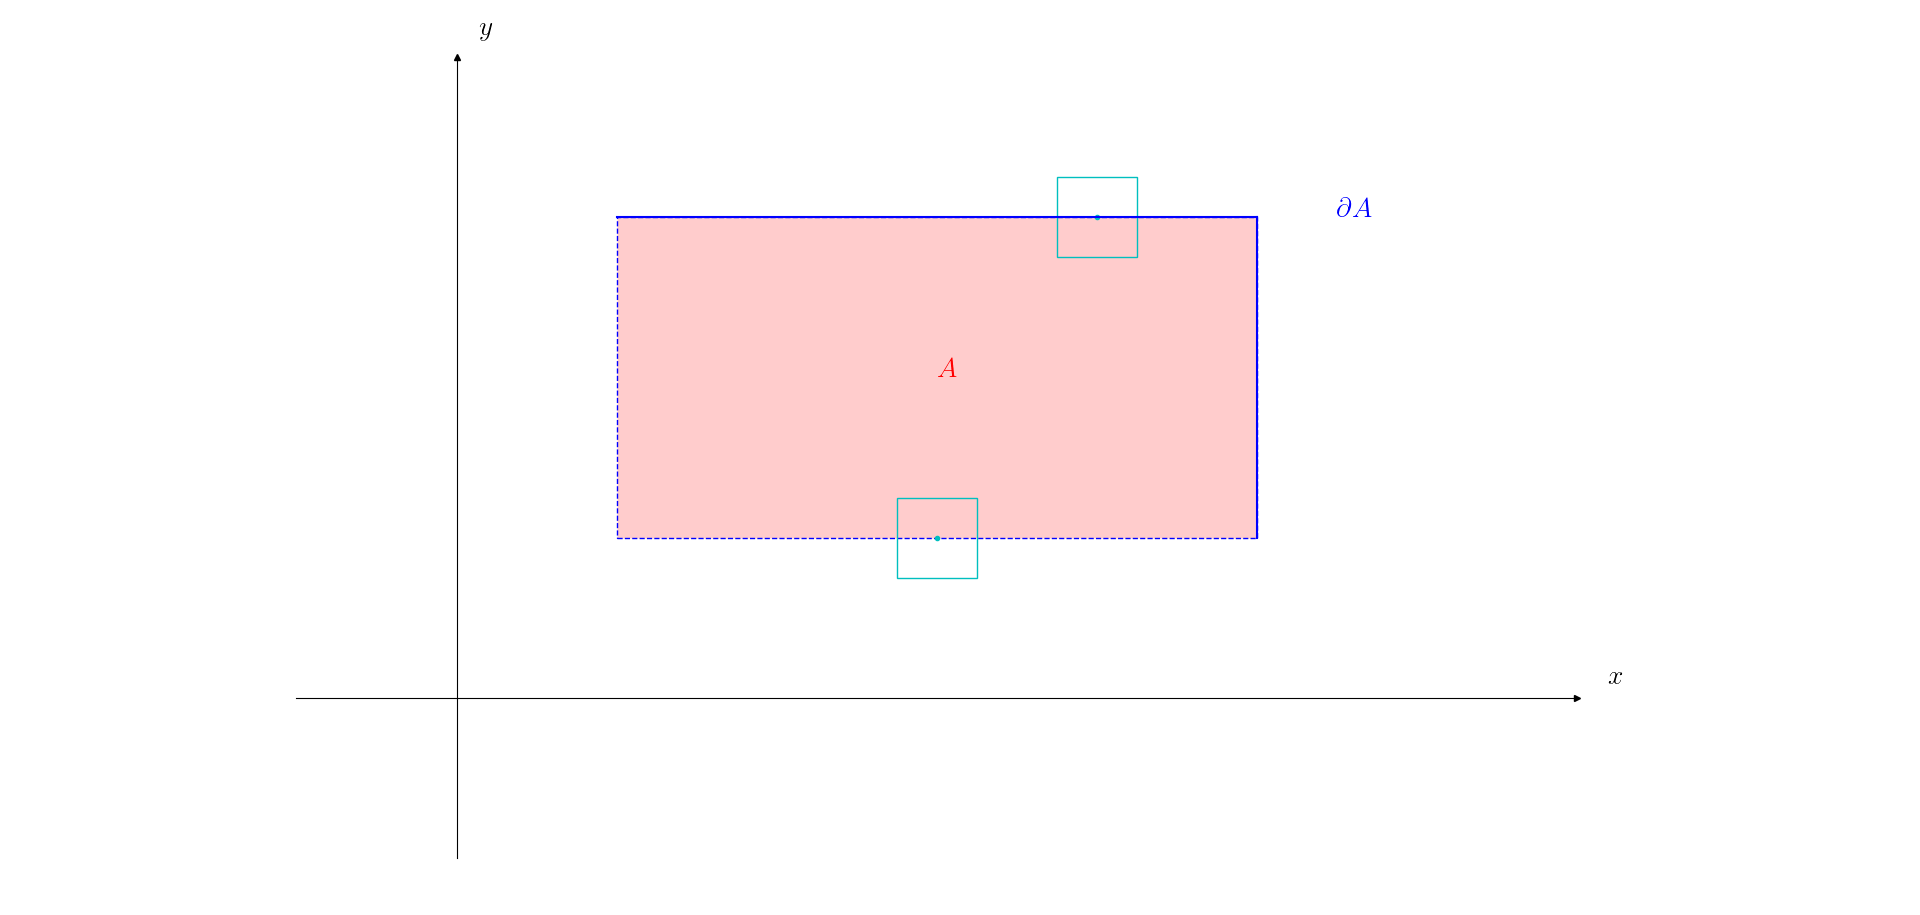
\includegraphics[width=0.65\linewidth]{spazi_metrici_e_normati/pag148}
	\label{fig:pag148}
\end{center}
\end{exbar}


\textbf{Osservazione:}

\begin{itemize}
\item $\partial A = \overline{A} \cap \overline{A^c}$
\begin{gather*}
	x \in \partial A \Rightarrow B_r (x) \cap A \neq \emptyset \qquad \forall \ r > 0, \; x \in \overline{A}
	\\
	\Rightarrow B_r(x) \cap A^c \neq \emptyset \qquad \forall r > 0, \; x \in \overline{A^c}
	\\
	\Rightarrow x \in \overline{A} \cap \overline{A^c} \Rightarrow \partial A \subseteq \overline{A} \cap \overline{A^c}
	\\
	x \in \overline{A} \cap \overline{A^c} \Rightarrow x \in \overline{A} \text{ e } x \in \overline{A^c}
	\\
	\begin{array}{c c}
		x \in \overline{A} \Rightarrow B_r(x) \cap A \neq \emptyset \quad \forall \ r > 0
		\\
		x \in \overline{A^c} \Rightarrow B_r(x)\cap A^c \neq \emptyset \quad \forall \ r > 0
	\end{array}
	\Rightarrow x \in \partial A
	\\
	\Rightarrow \overline{A} \cap \overline{A^c} \subseteq \partial A
\end{gather*}

\item $\overline{A}=A \cup \partial A$

\begin{equation*}
	A \subseteq \overline{A}, \; \partial A \subseteq \overline{A} \Rightarrow A \cup \partial A \subseteq \overline{A}
\end{equation*}
Facciamo vedere che $\overline{A} \subseteq A \cup \partial A$.
	
$x \in \overline{A}$, supponiamo che $x \notin A$ e dimostriamo che $x \in \partial A$
	
\begin{gather*}
	x \in \overline{A}  \Rightarrow \lowercomment{B_r(x) \cap A \neq \emptyset} {(x \notin A \Rightarrow x \in A^c)} {} \qquad \forall \ r > 0
	\\
	x \in B_r (x) \cap A^c \qquad \forall \ r > 0
	\\
	\mathcircled{B_r(x) \cap A^c \neq \emptyset \qquad \forall \ r > 0}
	\\
	\Rightarrow x \in \partial A, \text{ come si voleva}
\end{gather*}
\end{itemize}


\begin{attbar}
	$A$ è chiuso $\iff \partial A \subseteq A$, cioè se e solo se $A$ contiene la sua frontiera.
\end{attbar}


\begin{exbar}
\begin{example}
	$(\mathbb{R}, |\cdot|), \qquad \mathbb{Q} \subseteq \mathbb{R}$
	
	\begin{gather*}
		\overline{\mathbb{Q}} = \mathbb{R}
		\\
		\text{Fissati } x\in \mathbb{R} \text{ e }  r > 0 \quad \exists \ q \in \mathrm{Q} \text{ tale che }  q \in \ ]x-r, x+r[ \ = B_r(x)
		\\
		\partial \mathbb{Q} = \mathbb{R}
		\\
		x \in \mathbb{R}, \ B_r(x) \cap \mathbb{Q} \neq \emptyset \qquad \forall \ r > 0, B_r(x) \cap \ \mathbb{Q}^c \neq \emptyset \qquad \forall \ r > 0
		\\
		]x-r,x+r[ \ \cap \mathbb{Q}^c \neq \emptyset \qquad \forall \ r > 0
	\end{gather*}
	
	Se non fosse vero, $\exists \ x \in \mathbb{R}$ e $r > 0$ tale che $]x-r, x+r[$ è fatto tutto di numeri razionali.
	
	I razionali sono numerabili, cioè $\exists f: \mathbb{N} \rightarrow \mathbb{Q} $ iniettiva e suriettiva. I reali hanno la potenza del continuo, cioè ogni funzione $\phi: \mathbb{N} \rightarrow \mathbb{R}$ può essere al più iniettiva, ma non suriettiva. Questo è vero anche per ogni intervallo del tipo $]x-r, x+r[, r > 0$. Quindi, se $]x-r, x+r[$ fosse fatto di soli numeri razionali, sarebbe numerabile, assurdo.
\end{example}
\end{exbar}


\subsection{Successioni in spazi metrici}
\begin{exbar}
\begin{itemize}
	\item $\mathbb{R}^2 \qquad \{(e^{-n}, \frac{\sin n}{n}) \}_{n\geq 1}$ è una successione di elementi di $\mathbb{R}^2$
	\item $\mathbb{R}^3 \qquad \{ (1+\frac{1}{n}, \frac{\sinh n}{e^n},2^{-n}) \}$ è una successione di elementi di $\mathbb{R}^3$
\end{itemize}
\end{exbar}


\begin{definition}
	$\{x_k\}_{k\in \mathbb{N}} \subseteq X$ successione, con $(X,d)$ spazio metrico. 
	
	Si dice che $\{ x_k\}_{k \in \mathbb{N}}$ converge ad $x \in X$ e si scrive
	\begin{equation*}
		x_k \rightarrow x \qquad \text{o} \qquad \lim_{k\rightarrow +\infty} x_k = x \iff \lim_{k \rightarrow +\infty} d(x_k, x) = 0
	\end{equation*}
	
	(in ambito reale $\lim_{k \rightarrow +\infty} |x_k - x |=0$)
	
	cioè $\iff \forall \ \epsilon > 0 \ \exists \ N > 0 \ \big| \ k > N$
	
	$\Rightarrow d(x_k,x) < \epsilon$
	
	$x$ viene detto \textbf{limite della successione}.
	
\end{definition}


\begin{theorem}
	Sia $\{ x_k \}_{k \in \mathbb{N}} \subseteq X, (X,d)$ spazio metrico, tale che 
	\begin{equation*}
		x_k \rightarrow l_1 \in X \text{ e } x_k \rightarrow l_2 \in X
	\end{equation*}
	
	Allora $l_1=l_2$.
\end{theorem}


\begin{proposition}
	\label{pr:pag152}
	$\{\overline{x_k}\}_{k \in \mathbb{N}} \subseteq R^n$ tale che $\overline{x_k } = (x_{k_1}, x_{k_2}, \ldots, x_{k_n})$. Allora
	\begin{equation*}
		\overline{x_k} \rightarrow \overline{x} = (x_1, \ldots, x_n) \iff x_{k_{j}} \rightarrow x_{j} \qquad \forall \ j = 1, \ldots, n
	\end{equation*}
	
	cioè $\iff \forall \ j = 1, \ldots, n$ la successione di numeri reali $\{ x_{kj} \}_{k \in \mathbb{N}}$ converge a $x_{j}$.
\end{proposition}


\begin{exbar}

\begin{itemize}
	\item $\mathbb{R}^2, \left\{ \underbrace{ \left(e^{-k}, \frac{\sin k}{k} \right)} _ {\overline{x_k}} \right\}_{k \geq 1}$
	\begin{gather*}
		\overline{x_k} = (x_{k_1}, x_{k_2})
		\\
		\begin{array}{c c}
			x_{k_1} = e^{-k}, &
			x_{k_2} = \frac{\sin k}{k}
			\\
			\lim_{k \rightarrow +\infty} x_{k_1}=0, & \lim_{k \rightarrow +\infty} x_{k_2} = 0
		\end{array}
		\\
		\Rightarrow \lim_{k \rightarrow + \infty} \overline{x_k} = (0,0)
	\end{gather*}
	
	\item $\mathbb{R}^3, \left\{ \underbrace{ \left(1 + \frac{1}{k}, \frac{\sinh k}{e^k}, 2^{-k} \right)} _ {\overline{x_k}} \right\}_{k \geq 1}$
	\begin{gather*}
		\begin{array}{c c c}
		x_{k_1} = 1 + \frac{1}{k}, 
		& x_{k_2} = \frac{\sinh k}{e^k}, 
		& x_{k_3} = 2^{-k}
		\\
		\lim_{k \rightarrow +\infty} x_{k_1} = 1, \quad
		& \lim_{k \rightarrow +\infty} x_{k_2} = 1, \quad 
		& \lim_{k \rightarrow +\infty} x_{k_3} = 0 
	\end{array}
		\\
		\lim_{k \rightarrow +\infty} \overline{x_k} = (1, 1, 0)
	\end{gather*}

	\item $\mathbb{R}^2, \left\{ \underbrace{(2+e^{-k}, \sin k)} _ {\overline{x_k}} \right\} $
	\begin{gather*}
	\begin{array}{c c}
		x_{k1} = 2+e^{-k}, \quad 
		& x_{k2} = \sin k
		\\
		\lim_{k \rightarrow +\infty} x_{k_1} = 2, \quad 
		& \lim_{k \rightarrow +\infty} \nexists
	\end{array}
		\\
		\Rightarrow \lim_{k \rightarrow +\infty} \overline{x_k} \nexists
	\end{gather*}

\end{itemize}
\end{exbar}


\begin{dembar}
	\textbf{Dimostrazione} della \textbf{Proposizione \ref{pr:pag152}}
	
	
	$(\mathbb{R}^n, |\cdot|)$
	
	Se $\overline{y} = (y_1, \ldots, y_n) \in \mathbb{R}^n$, allora 
	\begin{gather*}
		|y_j| \leq |\overline{y}| \leq \sum_{i=1}^{n} |y_i| \qquad \forall \ j
		\\
		|y_j| = \sqrt{|y_j|^2} \leq \sqrt{\sum_{i=1}^{n} |y_i|^2} = |\overline{y}|
	\end{gather*}
	
	Abbiamo dimostrato che, se $0 < p < 1$, 
	\begin{equation*}
		(a+b)^p \leq a^p + b^p \qquad \forall \ a,b \geq 0
	\end{equation*}
	
	Questa disuguaglianza si può generalizzare.
	\begin{gather*}
		(a_1 + a_2 + \ldots + a_n)^p \leq a_1^p + a_2^p + \ldots + a_n^p \qquad \forall \ a_i \geq 0
		\\
		|\overline{y}| = \sqrt{\sum_{i=1}^{n} |y_i|^2} 
		\uppercomment{\leq} {p=\frac{1}{2}} {a_i = (y_1)^2} 
		(|y_1|^2)^{1/2} + (|y_2|^2)^{1/2} + \ldots + (|y_n|^2)^{1/2} =
		\\
		= |y_1| + |y_2| + \ldots + |y_n| = \sum_{i=1}^{n} |y_i|
		\\
		\uppercomment{|y_j|} {} {y_j = x_{k_{j}} - x_j}
		\leq |\overline{y}| \leq \sum_{i=1}^{n} |y_i|
		\\
		\overline{x_k} \rightarrow \overline{x} \iff x_{k_j} \rightarrow x_j \qquad \forall \, j = 1, \ldots, n
		\\
		|x_{k_{j}} - x_j| \leq |\overline{x_k} - \overline{x}| \leq \sum_{i=1}^{n} |x_{k_i} - x_i|
	\end{gather*}

	Se $|\overline{x_k} - \overline{x}| \rightarrow 0 $, cioè se $\overline{x_k} \rightarrow \overline{x}$, allora
	\begin{equation*}
		0 \leq \lowercomment{|x_{kj}-x_j|} {\myarrow[270]} {0 \text{ per confronto}} \leq |\overline{x_k} - \overline{x}| \Rightarrow x_{k_{j}} \rightarrow x_j \qquad \forall \ j
	\end{equation*}
	
	D'altra parte, se $x_{k_{i}} \rightarrow  x_i \quad \forall \ i = 1, \ldots, n$
	\begin{gather*}
		\Rightarrow \sum_{i=1}^{n} |x_{k_i} - x_i| \rightarrow 0 \text{ per } k \rightarrow + \infty
		\\
		\Rightarrow 0 \leq |x_{k} - x| \leq \sum_{i=1}^{n} |x_{k_{i}} - x_i| \Rightarrow \overline{x_k} \rightarrow \overline{x} \qquad \square
	\end{gather*}	
\end{dembar}


\begin{theorem} (caratterizzazione dei chiusi mediante le successioni)
\label{th:pag 156}	
	
$(X,d)$ spazio metrico, $A \subseteq X$. Allora $z \in \overline{A} \iff \exists$ una successione $\{x_k\}_{k \geq 1} \subseteq A \ \big| \ x_k \rightarrow z$.
\end{theorem}


\begin{corollary}
	\label{cor:pag 156}
	$(X,d)$ spazio metrico. $A \subseteq X$ è chiuso $\iff \forall \ \{x_k\}_{k \geq 1} \subseteq A$ convergente, il suo limite appartiene ad $A$.
	
	($A \subseteq X$ è chiuso $\iff A$ contiene i limiti delle successioni convergenti a valori in $A$.)
\end{corollary}


\begin{dembar}
	\textbf{Dimostrazione} del \textbf{Corollario \ref{cor:pag 156}}
	
	\begin{itemize}
		\item $(\Rightarrow) \ A$ chiuso, $A = \overline{A}$. Sia $\{x_k\}_{k \geq 1} \subseteq A$ successione convergente a $z \in X$.
		
		Allora il teorema implica che $z \in \overline{A}= A$.
		
		\item $(\Leftarrow)$ Dobbiamo dimostrare che, se $x \in \overline{A}$, allora $z \in A$
		
		($A = \overline{A}$, perché l'inclusione $A \subseteq \overline{A}$ è nota)
		
		$z \in \overline{A} \Rightarrow \exists \ \{x_k\}_{k \geq 1} \subseteq A$ convergente a $z$. 
		
		Allora $z \in A$ per ipotesi. $\qquad \square$
	\end{itemize}
\end{dembar}


\begin{dembar}
	\textbf{Dimostrazione} del \textbf{Teorema \ref{th:pag 156}}
	
	\begin{itemize}
		\item $(\Rightarrow ) $ Sia $z \in \overline{A}$. Costruiamo una successione $\{x_k\}_{k \geq 1} \subseteq A \ \big| \ x_k \rightarrow z$
		\begin{gather*}
		z\in \overline{A} \iff \forall \ r > 0, B_r(z) \cap A \neq \emptyset
		\\
		\begin{array}{c c}
			r = 1 
			& \exists \ x_1 \in B_1(z) \cap A 
			\\ & x_1 \in A \text{ e } d(x_1, z) < 1
			\\
			r = \frac{1}{2}
			& \exists \ x_2 \in B_{1/2}(z) \cap A
			\\ & x_2 \in A \text{ e } d(x_2, z )< \frac{1}{2}
			\\
			\vdots & \\
			r=\frac{1}{k}
			& \exists \ x_k \in B_{\frac{1}{k}}(z) \cap A,
			\\ & x_k \in A \text{ e } d(x_k, z) < \frac{1}{k}
		\end{array}
		\\
		\{x_k\}_{k \geq 1} \subseteq A \ \big| \; 0 \leq d(x_k, z) \leq \frac{1}{k} 
		\\ \Rightarrow \lim_{k \rightarrow +\infty} d(x_k, z) = 0 \Rightarrow x_k \rightarrow z
		\end{gather*}
		
		\item $(\Leftarrow )$ Ipotesi: $\exists \ \{x_k\}_{k\geq 1} \subseteq A \ \big| \ x_k \rightarrow z$
		
		Tesi: $z \in \overline{A}$
		
		Sia $r >0$. Poiché $x_k \rightarrow z$
		\begin{gather*}
		\exists \ N > 0 \ \big| \; d(x_k,z) < r \qquad \forall \ k > N, \lowercomment{x_k} {\in A} {} \in B_r(z) \cap A
		\\
		\Rightarrow B_r(z) \cap A \neq \emptyset \Rightarrow z \in \overline{A}. \qquad \square
		\end{gather*} 
	\end{itemize}
\end{dembar}


\begin{exbar}
	\begin{itemize}
		\item $\mathbb{Q}$ non è chiuso in $\mathbb{R}$ perché $\exists \ \{q_n\}_{n\geq 1} \subseteq \mathbb{Q} \ \big| \ q_n \rightarrow \sqrt{2} \neq \mathbb{Q}$
		
		\item $(\mathbb{R}^2, |\cdot|)$
	\end{itemize}	
	\begin{center}
		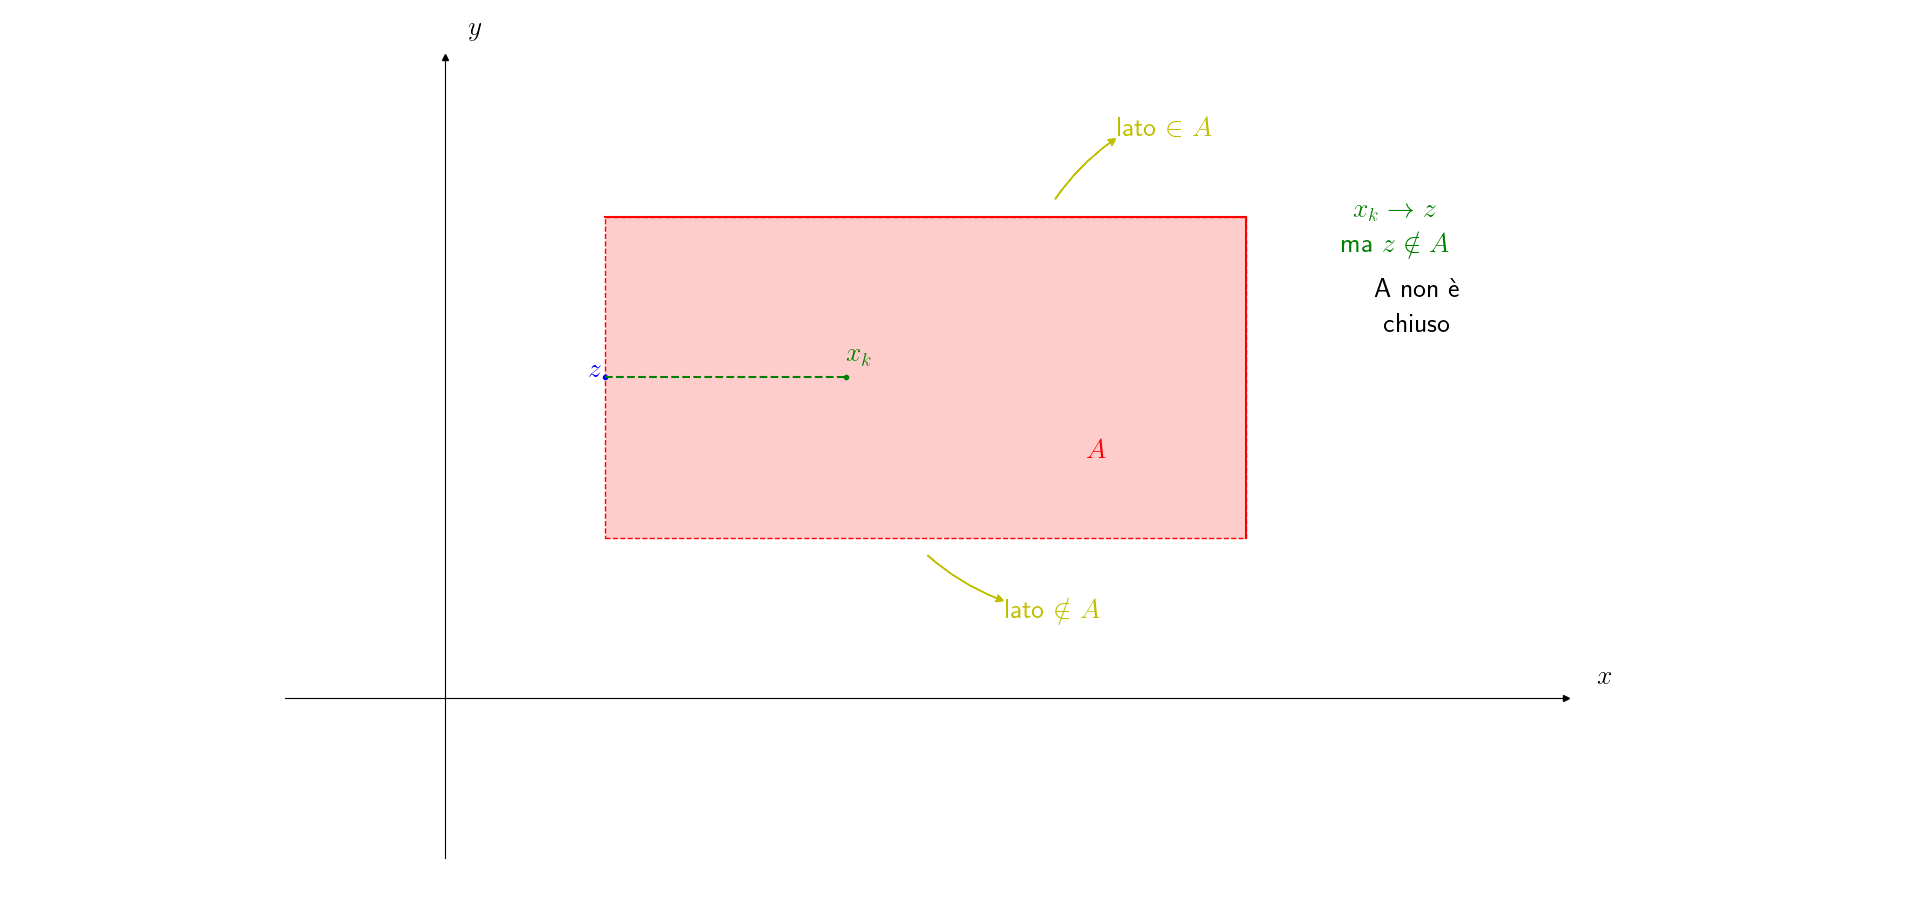
\includegraphics[width=0.75\linewidth]{spazi_metrici_e_normati/pag159}
		\label{fig:pag159}
	\end{center}	
\end{exbar}


\begin{exbar}
\begin{example} \textbf{importante}
	
	$C \subseteq \mathbb{R}^n$. Sono equivalenti le seguenti affermazioni
	\begin{enumerate}
		\item $C$ è chiuso per la topologia data dalla norma euclidea $|\cdot|$
		
		\item $C$ è chiuso per la topologia data dalla norma $\parallel \cdot \parallel_\infty$
		
		\item $C$ è chiuso per la topologia data dalla norma $\parallel \cdot \parallel_1$
	\end{enumerate}
	
	Per dimostrare che le tre affermazioni sono equivalenti, partiamo da
	\begin{gather*}
		|x_j| \leq |\overline{x}| \leq \sum_{i=1}^{n} |x_i| \qquad \forall \ \overline{x} = (x_1, \ldots, x_n) \in \mathbb{R}^n
		\\
		\lowercomment{\max_{j = 1, \ldots, n} |x_j|} {= \parallel \overline{x} \parallel_\infty} {}
		\leq |\overline{x}| \leq 
		\lowercomment{\sum_{i=1}^{n} |x_i|} {= \parallel \overline{x} \parallel_1} {} 
		\leq n \lowercomment{\max_{j = 1, \ldots, n} |x_j|} {= \parallel \overline{x} \parallel_\infty} {}
		\\
		\parallel \overline{x} \parallel_\infty \leq |\overline{x}| \leq \parallel \overline{x} \parallel_1 \leq n \parallel \overline{x} \parallel_\infty \qquad \forall \ \overline{x} \in \mathbb{R}^n
	\end{gather*}
	
	\begin{itemize}
		\item $1) \Rightarrow 2)$ 
		
		Ipotesi: $C$ è chiuso per $|\cdot|$. 
		
		Tesi: $C$ è chiuso per $ \parallel \cdot \parallel_\infty$
		
		$\{ \overline{x_k} \}_{k\geq 1} \subseteq C \ \big| \ \overline{x_k} \rightarrow \overline{z}$ per $\parallel \cdot \parallel_\infty$, cioè $\parallel \overline{x_k} - \overline{z} \parallel_\infty \rightarrow 0 $ per $k \rightarrow +\infty$, e dimostriamo che $\overline{z} \in C$
		\begin{equation*}
			|\overline{x_k} - \overline{z}| \lowercomment{\leq} {\text{disuguaglianza sopra}} {\text{con } \overline{x} = \overline{x_k} - \overline{z}}
			n \parallel \overline{x_k}-\overline{z} \parallel_\infty \rightarrow 0
		\end{equation*}
		
		$\Rightarrow |\overline{x_k} - \overline{z}| \rightarrow 0$ per $k \rightarrow +\infty$, cioè $\overline{x_k} \rightarrow \overline{z}$ per $|\cdot|$. Ma $C$ è chiuso per $|\cdot| \Rightarrow \overline{z} \in \mathbb{C}$.
		
		\item $2) \Rightarrow 3)$
		
		Ipotesi: $C$ è chiuso per $\parallel \cdot \parallel_\infty$.
		
		Tesi: $C$ è chiuso per $\parallel \cdot \parallel_1$
		
		$\{ \overline{x_k} \}_{k \geq 1} \subseteq C \ \big| \ \overline{x_k} \rightarrow \overline{z}$ per $\parallel \cdot \parallel_1$, cioè $\parallel \overline{x_k} - \overline{z} \parallel_1 \rightarrow 0$ per $k \rightarrow +\infty$ e dimostriamo che $\overline{z} \in C$.
		\begin{equation*}
			\parallel \overline{x} \parallel_\infty \leq \parallel \overline{x} \parallel_1 \qquad \forall \ \overline{x}\in \mathbb{R}^n
		\end{equation*}

		Prendo $\overline{x} = \overline{x_k} -\overline{z}$
		
		\begin{gather*}
			\parallel \overline{x_k} - \overline{z} \parallel_\infty \leq  \parallel \overline{x_k} -\overline{z} \parallel_1 \rightarrow 0 \Rightarrow \overline{x_k}  \rightarrow \overline{z} \text{ per } \parallel \cdot \parallel_\infty \rightarrow \overline{z} \in \mathbb{C}
		\end{gather*}
	
		perché $C $ è chiuso  per $\parallel \cdot \parallel_\infty$.
		
		\item $3) \Rightarrow 1)$ 
		
		Ipotesi: $C$ è chiuso per $\parallel \cdot \parallel_1$. 
		
		Tesi: $C$ è chiuso per $|\cdot|$
		
		$\{ \overline{x_k}\}_{k \geq 1} \subseteq C \ \big| \ \overline{x_k} \rightarrow \overline{z}$ per $|\cdot|$ e dimostriamo che $\overline{z} \in C$ 
		\begin{gather*}
			\parallel \overline{x} \parallel_1 \leq n \parallel \overline{x} \parallel_\infty \qquad \forall \ \overline{x} \in \mathbb{R}^n
			\\
			\frac{1}{n} \parallel \overline{x} \parallel_1 \leq \parallel \overline{x}\parallel_\infty \leq |\overline{x}| \qquad \forall \ \overline{x} \in \mathbb{R}^n
			\\
			\parallel \overline{x} \parallel_1 \leq n |\overline{x}| \qquad \forall \ \overline{x} \in \mathbb{R}^n
			\\
			\overline{x} = \overline{x_k} - \overline{z}
			\\
			\Rightarrow \parallel \overline{x_k} - \overline{z} \parallel_1 \leq n |\overline{x_k} - \overline{z}| \rightarrow 0 \text{ per } k \rightarrow +\infty
			\\
			\Rightarrow \parallel \overline{x_k} - \overline{z} \parallel_1 \rightarrow 0 \text{ per } k \rightarrow +\infty
			\\
			\Rightarrow \overline{x_k} - \overline{z} \text{ per } \parallel \cdot \parallel_1 \Rightarrow z \in C
		\end{gather*}
		
		perché $C$ è chiuso per $\parallel \cdot \parallel_1$.
	\end{itemize}
\end{example}
\end{exbar}


\textbf{Osservazione:}

Siccome $C$ è chiuso $\iff C^c$ è aperto, il corollario al teorema che abbiamo appena dimostrato implica che $A \subseteq R^n$ è aperto per $|\cdot|  \iff A $ è aperto per la topologia data da $\parallel \cdot \parallel_\infty \iff A$ è aperto per $\parallel \cdot \parallel_1$, cioè le 3 norme $|\cdot|$, $\parallel \cdot \parallel_\infty$, $\parallel \cdot \parallel_1$ descrivono la stessa topologia.

\begin{attbar}
	Si può dimostrare che in $\mathbb{R}^n$ (spazio di dimensione finita) tutte le norme sono equivalenti, cioè se $A \subseteq \mathbb{R}^n$ è aperto per una norma, lo è per qualsiasi altro.
\end{attbar}


\begin{definition}
	$(X,d)$ spazio metrico. $K \subseteq X$ si dice limitato se $\exists \ x \in X$ e $R>0 \ \big| \ K \subseteq B_R(x)$, cioè $d(x,z) < R \qquad \forall \ z \in K$. 
\end{definition}


\begin{exbar}
	$K \subseteq \mathbb{R}$ è limitato se $\exists R > 0 \ \big| \ K \subseteq \ ]-R, R \ [ \ = B_R(0)$ cioè $|z| < R \quad \forall \ z \in K$.
\end{exbar}


\textbf{Osservazione:}
Se $(X, \parallel \cdot \parallel)$ è spazio normato, il punto $x \in X$ nella definizione di insieme limite può essere preso coincidente con $0$. 

Infatti se $k \subseteq B_R(x)$
\begin{gather*}
	\Rightarrow \lowercomment{ \parallel x-z \parallel} {= d(x,z)} {} < R \qquad \forall \ z \in K
	\\
	z \in K \qquad \parallel z \parallel = \parallel z - x + x \parallel \distr \parallel x-z \parallel + \parallel x\parallel < R + \parallel x \parallel \\
	\Rightarrow z \in B_{R + \parallel x \parallel}(0)
\end{gather*}

Quindi, in uno spazio normato, $K \subseteq X$ è limitato se $\exists \ R >0 \ \big| \ K \subseteq B_R(0)$, cioè $\parallel z \parallel < R \quad \forall \ z \in K$. 

(se $x = R$ e $\parallel \cdot \parallel = |\cdot|$, si ritrova quanto scritto sopra.)


\begin{proposition}

	$(X,d)$ spazio metrico. $\{ x_k \}_{k\geq 1} \subseteq X$ successione convergente. Allora $\{ x_k \}_{k \geq 1}$ è limitata, cioè $\exists x \in X$ e $R >0 \ \big| \ x_k \in B_R(x) \quad \forall \ k \geq 1$
	
	$(d(x_k,x)< R \quad \forall \ k \geq 1)$
\end{proposition}


\begin{exbar}
\begin{example}
	$C^0 ([0,1])$
	
	$K = \{ f \in C^0 ([0,1]) \ \big| \ |f(x)| \leq \frac{1}{\sqrt{x}} \qquad \forall x \in \ ]0,1] \}$
	\begin{itemize}
		\item $(C^0 ([0,1]), \parallel \cdot \parallel_1)$, $K$ è limitato 
		\begin{gather*}
			f \in K \qquad \parallel f \parallel_1 = \int_{0}^{1} |f(x)| \ \mathrm{d}x \leq \int_{0}^{1} \frac{1}{\sqrt{x}} \ \mathrm{d}x = \lim_{c \rightarrow 0^+} \int_{c}^{1} \frac{1}{\sqrt{x}} \ \mathrm{d}x = 2
			\\
			\parallel f \parallel_1 \leq 2 \qquad \forall \ f \in K
			\\
			K \subseteq \overline{B_{2}^{\parallel \cdot \parallel_1}(0)} \subseteq B_{3}^{\parallel \cdot \parallel_1}(0)
		\end{gather*}

		\item ($C^0 ([0,1]), \parallel \cdot \parallel_\infty$), $K$ è illimitato
		
		\begin{center}
			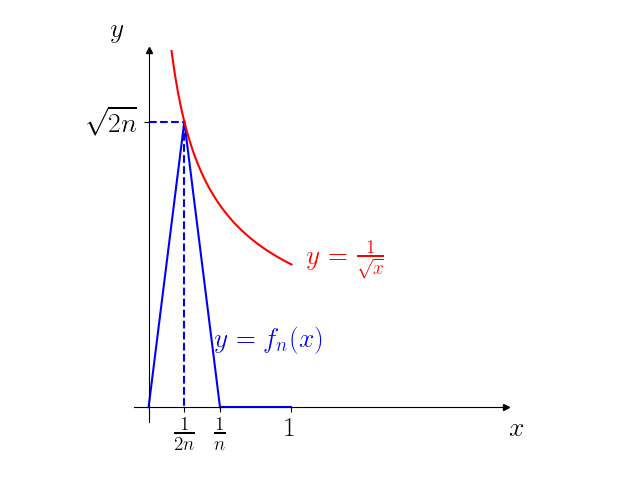
\includegraphics[width=0.7\linewidth]{spazi_metrici_e_normati/pag165}
			\label{fig:pag165}
		\end{center}
		
		$\parallel f_n \parallel_\infty = \sqrt{2n} \rightarrow +\infty \text{ se } n \rightarrow +\infty, \quad f_n \in K$
		
		\item $C^0 ([0,1]), \{ f_n \}_{n \geq 1}$ come sopra. Allora $f_n \rightarrow f = 0$ per $\parallel \cdot \parallel_1$
		\begin{gather*}
			\parallel f_n - 0 \parallel_1 =\int_{0}^{1} |f(x)| \mathrm{d}x = \frac{1}{n} \ \sqrt{2n} \ \frac{1}{2} = \frac{1}{\sqrt{2n}} \rightarrow 0 \textbf{ per } n \rightarrow +\infty
			\\
			\text{Ma } \parallel f_n - 0 \parallel_\infty = \sqrt{2n} \rightarrow +\infty \Rightarrow f_n \nrightarrow 0 \text{ per } \parallel \cdot \parallel_\infty
		\end{gather*}
	\end{itemize}
\end{example}
\end{exbar}


\textbf{Osservazione:}
$K \subseteq \mathbb{R}^n$ è limitato per $|\cdot| \iff$ lo è per $\parallel \cdot \parallel_\infty \iff$ lo è per $\parallel \cdot \parallel_1$
\begin{equation*}
	\parallel \overline{x} \parallel_\infty \leq |\overline{x}| \leq \parallel \overline{x} \parallel_1 \leq n \parallel \overline{x} \parallel_\infty
\end{equation*}


\begin{center}
	\label{fig:pag166_1}
	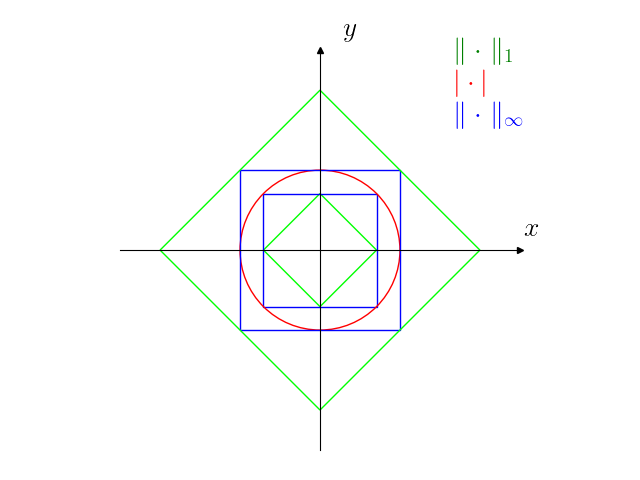
\includegraphics[width=0.7\linewidth]{spazi_metrici_e_normati/pag166_1}
\end{center}


\textbf{Osservazione:}
Introduciamo in $\mathbb{R}^n$ il simbolo $\infty$. Un intorno di $\infty$ è un qualunque insieme $A \subseteq \mathbb{R}^n \; \big| \; A$ contiene il complementare di una palla di centro l'origine, cioè $\exists \ R > 0 \; \big| \; \overline{x} \in A \Rightarrow \parallel \overline{x} \parallel > R$
\begin{center}
	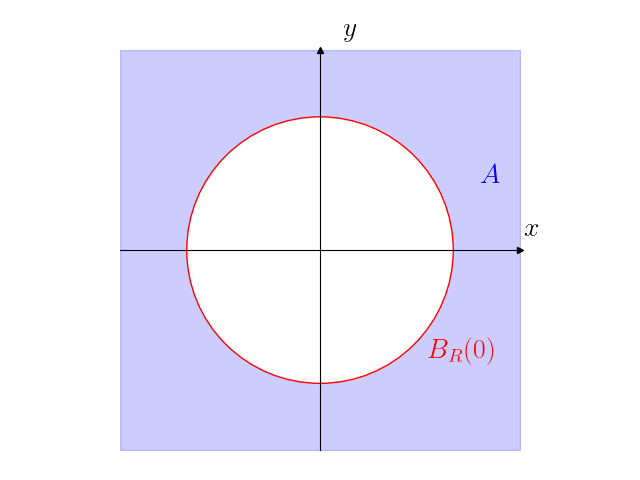
\includegraphics[width=0.7\linewidth]{spazi_metrici_e_normati/pag166_2}
	\label{fig:pag1662}
\end{center}

Una successione $\{\overline{x_k}\}_{k \geq 1} \subseteq \mathbb{R}^n$ si dice divergente a $\infty$ e si scrive $\lim_{k} \overline{x_k} = \infty$ se $\lim_{k} |\overline{x_k}| = +\infty$ cioè se $\forall \ R > 0 \; \exists \ N > 0 \; \big| \; k > N \Rightarrow |\overline{x_k}| > R$


\begin{exbar}
\begin{example}
\begin{gather*}
\overline{x_k} = (\lowercomment{e^{-k}} {x_{k1}} {}, \lowercomment{2+\frac{1}{k}} {x_{k2}} {}, \lowercomment{\ln k} {x_{k3}} {}) \subseteq \mathbb{R}^3, \qquad k \geq 1
\\
\lim_{k} x_{k1} = \lim_{k} e^{-k} = 0
\\
\lim_{k} x_{k2} = \lim_{k} 2 + \frac{1}{k} = 2
\\
\lim_{k} x_{k3} = \lim_{k} \ln k = +\infty
\\
\lim_{k} |\overline{x_k}| = \lim_{k} \sqrt{e^{-2k} + \bigg(2+\frac{1}{k} \bigg)^2 + (\ln k)^2} = +\infty \Rightarrow \lim_{k} \overline{x_k} = \infty
\end{gather*}
\end{example}
\end{exbar}


\subsection{Limiti di funzione}
\begin{definition}
	$(X,d)$ spazio metrico, $A \subseteq X$, non vuoto. $x_0 \in X$ si dice \textbf{punto di accumulazione} per $A$ se  $\forall \epsilon >0 \ \exists \ x \in A, x \neq x_0,$ tale che $x \in B_\epsilon(x_0)$, cioè se $B_\epsilon (x_0) \cap A$ contiene punti di $A$ diversi da $x_0$. 
	
	$x_0 \in A$ si dice \textbf{punto isolato} se non è di accumulazione, cioè se $\exists \epsilon > 0$ tale che $B_\epsilon (x_0) \cap A =\{ x_0 \}$.
\end{definition}


\begin{definition}
	$(X,d_x),(Y,d_y)$ spazi metrici, $f:dom \ f \rightarrow Y$, con $dom \ f \subseteq X, x_0 \in X $ punto di accumulazione per $dom \ f$. Si dice che $f$ ha limite $\ell \in Y$ per $x \rightarrow x_0$ e si scrive
	\begin{equation*}
	\begin{array}{r l}
		\lim_{x \rightarrow x_0} f(x) = \ell & \text{oppure}
		\\
		f(x) \rightarrow \ell & \text{per } x \rightarrow x_0
	\end{array}
	\end{equation*}
	se per ogni intorno  $V$ di $\ell$  esiste un intorno $U$ di $x_0 \; \big| \; f(x) \in V, \ x \in U \cap dom \ f, x \neq x_0 $
	
	In altre parole, $\lim_{x \rightarrow x_0} f(x) = \ell \quad \forall \ \epsilon > 0 \quad \exists \ \delta > 0 \; \big| $ se $ 0 < \lowercomment{d_x(x, x_0)} {x \in B_\delta^x(x_0)} {} < \delta$ e $x \in dom \ f $, allora $\lowercomment{d_y (f(x), \ell)} {f(x) \in B_\epsilon^y(\ell)} {} < \epsilon$ 
	
	(Se prendo la definizione data con $\epsilon$ e $\delta$ per $X = Y = \mathbb{R}$ e le distanze $d_x(x,y) = d_y(x,y) = |x-y|$, ottengo la definizione con $\epsilon$ e $\delta$ data in ambito reale.)
\end{definition}


\begin{theorem} (di unicità del limite)
	
	$(X,d_x)$ e $(Y,d_y)$ spazi metrici, $f : dom \ f \rightarrow Y, \ dom \ f \subseteq X, \ x_0 \in X$ punto di accumulazione per $dom \ f$.
	
	Se $\lim_{x \rightarrow x_0} f(x) = \ell_1 \in Y$ e $\lim_{x \rightarrow x_0} f(x) = \ell_2 \in Y$, allora $\ell_1 = \ell_2$.
\end{theorem}


\begin{proposition}
	$(X,d)$ spazio metrico, $\overline{f}: dom \ \overline{f} \rightarrow \mathbb{R}^n, \qquad \overline{f}(x) = \big(f_1(x), \ldots, f_n(x) \big), \ x_0 \in X$ punto di accumulazione per $dom \ \overline{f} \subseteq X$, allora 
	\begin{equation*}
		\lim_{x \rightarrow x_0} \overline{f}(x) = \overline{\ell} = (\ell_1, \ldots, \ell_n) \in \mathbb{R}^n \iff \lim_{x \rightarrow x_0} f_j(x) = \ell_j \qquad \forall j = 1, 2, \ldots, n
	\end{equation*}
\end{proposition}


\begin{theorem} (della permanenza del segno)
	
	$(X,d)$ spazio metrico, $f: dom \ f \rightarrow \mathbb{R}, \ dom \ f \subseteq X, \ x_0 \in X$ punto di accumulazione per $dom \ f$.
	
	Se $\lim_{x \rightarrow x_0} f(x) = \ell > 0$, allora $f(x) > 0$ definitivamente per $ x \rightarrow x_0$, cioè $\exists \ \delta > 0 \; \big| \; f(x) > 0 \ \forall \ x \in B_\delta (x_0) \cap dom \ f, \ x \neq x_0$. 
\end{theorem}


\begin{theorem}
	$(X,d)$ spazio metrico, $f,g: A \rightarrow \mathbb{R}, \ A \subseteq X, \ x_0 \in X$ punto di accumulazione per $A$, tali che $\lim_{x \rightarrow x_0} f(x) = \ell_f, \ \lim_{x \rightarrow x_0} g(x) = \ell_f$ e $f(x) \leq g(x)$ definitivamente per $x \rightarrow x_0$. ($\exists \ \delta > 0 \; \big| \; f(x) \leq g(x) \forall x \in B_\delta (x_0) \cap A$, \ $x \neq x_0$.)
	
	Allora $\ell_f \leq \ell_g$.
\end{theorem}


\begin{theorem}(del confronto o dei due carabinieri)
	
	$(X,d)$ spazio metrico, $f,g,h : A \rightarrow \mathbb{R}, \ A \subseteq X, x_0$ punto di accumulazione per $A$, tali che $g(x) \leq f(x) \leq h(x)$ definitivamente per $x \rightarrow x_0$. 
	
	Se $\lim_{x \rightarrow x_0} g(x) = \lim_{x \rightarrow x_0} h(x) = \ell$, allora $\lim_{x \rightarrow x_0} f(x) = \ell$.
\end{theorem}


\subsection{Funzioni continue tra spazi metrici}

\begin{definition}	
	$(X,d_x), \ (Y,d_y)$ spazi metrici, $f:dom \ f \rightarrow Y, \ dom \ f \subseteq X$, si dice \textbf{continua in } $\mathbf{x_0 \in dom \ f}$ se vale una delle due
	\begin{enumerate}
		\item $x_0$ è punto isolato per $dom \ f$
		\item $\lim_{x \rightarrow x_0} f(x) = f(x_0)$
	\end{enumerate}
	
	In altre parole, $f$ è continua in $x_0$ se $\forall \ \epsilon > 0 \ \exists \ \delta > 0 \; \big| \; \text{ se } d_x(x, x_0) < \delta \text{ e } x \in dom \ f$, allora $d_y(f(x), f(x_0) < \epsilon$. 
	

	$\bigg( \begin{array}{l}
	x \in B_{\delta}^{x}(x_0) \cap dom \ f \Rightarrow f(x) \in B_{\epsilon}^{y} (f(x_0)) \Rightarrow x \in f^{-1}(B_{\epsilon}^{y} (f(x_0)))$
	\\
	$\forall \ \epsilon > 0 \ \exists \ \delta > 0 \; \big| \; B_{\delta}^{x}(x_0) \cap dom \ f \subseteq f^{-1} (B_{\epsilon}^{y} (f(x_0)))
	\end{array}
	\bigg)$
	
	Una funzione $f:dom \ f \rightarrow Y $ si dice continua se è continua in ogni punto del suo dominio.
\end{definition}


\begin{theorem}
	\label{th: pag172}
	$(X,d_x), \ (Y,d_y)$ spazi metrici, $f:X \rightarrow Y$. $f$ è continua $\iff f^{-1}(A)$ è aperto (in $X$) per ogni aperto $A \subseteq Y$.
\end{theorem}


\begin{dembar}
\textbf{Dimostrazione} del \textbf{Teorema \ref{th: pag172}}

	
	\begin{itemize}
		\item $\Rightarrow)$ Ipotesi: $f$ continua.
		
		Tesi: Dato $A \subseteq Y$ aperto, $f^{-1}(A)\subseteq X$ è aperto.
		
		Sia $x_0 \in f^{-1}(A)$. Dobbiamo trovare una palla centrata in $x_0$ contenuta in $f^{-1}(A)$.
		
		$f(x_0) \in A$, che è aperto, 
		\begin{gather*}
			\exists \ \epsilon >0 \; \big| \; B_{\epsilon}^{Y} (f(x_0)) \subseteq A
			\\
			\exists \ \delta > 0 \; \big| \; B_{\delta}^{X} (x_0) \Rightarrow f(x) \in B_{\epsilon}^{Y} (f(x_0)) \subseteq A
			\\
			B_{\delta}^{X}(x_0) \subseteq f^{x_0} (A) \text{, come si voleva.}
		\end{gather*}
		\item $\Leftarrow)$ Ipotesi: $f^{-1}(A) \subseteq X$ è aperto $\forall A \subseteq Y$ aperto. Tesi: $f$ è continua
		
		Fissiamo $x_0 \in X$ e $\epsilon > 0$.
		
		Dobbiamo trovare $\delta > 0 \; \big| \; x \in B_{\delta}^{X} (x_0) \Rightarrow f(x) \in B_{\epsilon}^{Y} (f(x_0))$
		
		\begin{gather*}
			B_{\epsilon}^{y} (f(x_0)) \text{ è un aperto } \Rightarrow f^{-1}(B_{\epsilon}^{Y} (f(x_0))) \text{ è aperto e } x_0 \in f^{-1} (B_{\epsilon}^{Y} (f(x_0))) 
			\\
			\Rightarrow \exists \ \delta > 0 \; \big| \; B_{\delta}^{X} (x_0) \subseteq f^{-1} (B_{\epsilon}^{Y}(f(x_0))) 
			\\
			\text{ cioè, se } x \in B_{\delta}^{X}(x_0) \Rightarrow f(x) \in B_{\epsilon}^{Y} (f(x_0)) \text{ come si voleva.} \qquad \square
		\end{gather*}
		
	\begin{center}
		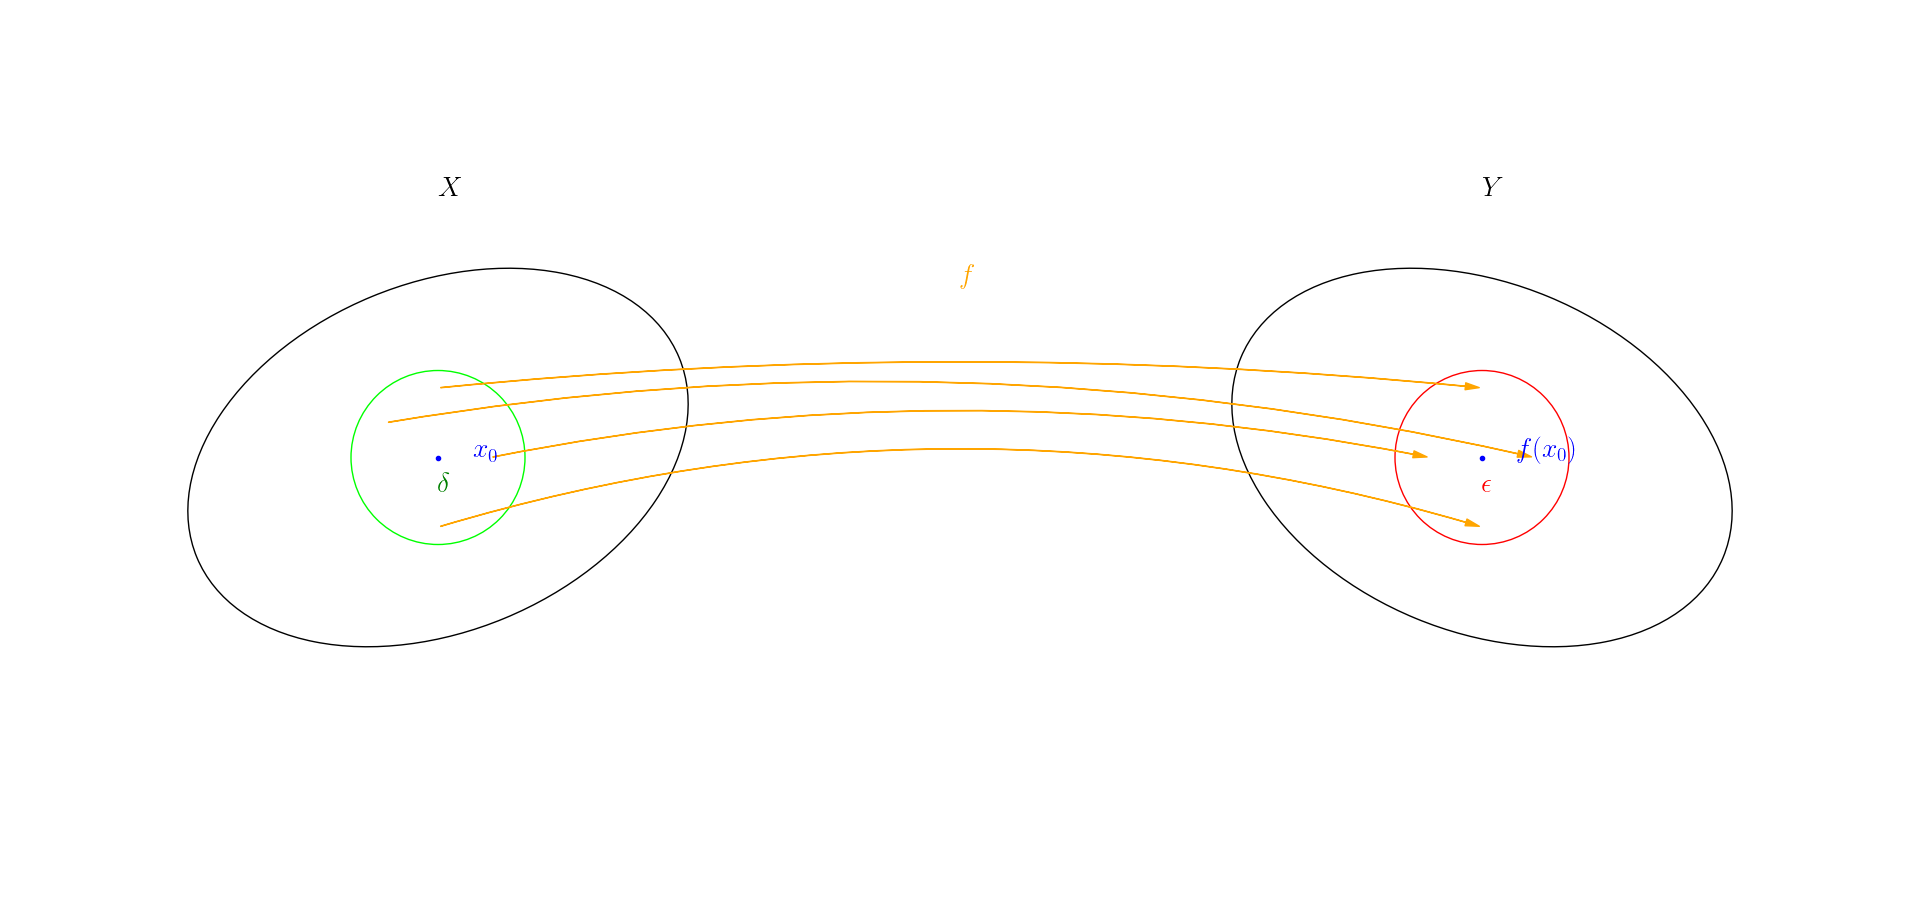
\includegraphics[width=0.7\linewidth]{spazi_metrici_e_normati/pag174}
		\label{fig:pag174}
	\end{center}
	\end{itemize}
\end{dembar}


\begin{theorem}
	$(X,d)$ spazio metrico. $A \subseteq X, \ f,g: A \rightarrow \mathbb{R}, \ x_0 \in A$, $f$ e $g$ continue in $x_0$. Allora $f + g, f \cdot g$ e $f / g$, se $g(x_0) \neq 0$, sono continue in $x_0$.
\end{theorem}


\begin{proposition}
	$(X,d)$ spazio metrico, $A \subseteq X, \overline{f}: A \rightarrow \mathbb{R}^n, \ \overline{f}(x) = (f_1(x), \ldots, f_n(x))$, è continua in $x_0 \in A \iff$ sono continue in $x_0$ le sue componenti $f_j \qquad \forall j = 1, \ldots, n$.
\end{proposition}


\begin{exbar}
\begin{example}
	$(X,d_x),(Y,d_y)$ spazi metrici.
	\begin{enumerate}
		\item Provare che \begin{gather*}
			d((x_1,y_1), (x_2,y_2)) = \sqrt{(d_x(x_1,x_2))^2 + (d_y(y_1,y_2))^2}
			\\
			(x_1, y_1), (x_2,y_2) \in X \times Y \text{ è una metrica in } X \times Y
		\end{gather*}
		
		\item Provare che $\forall r > 0$ vale
		\begin{equation*}
			B_{\frac{r}{\sqrt{2}}}^{X}(x) \times B_{\frac{r}{\sqrt{2}}}^{Y}(y) \subseteq B_{r}^{X \times Y} ((x_0,y_0)) \subseteq B_{r}^{X} (x_0) \times B_{r}^{Y} (y_0)
		\end{equation*}
		
		\begin{center}
			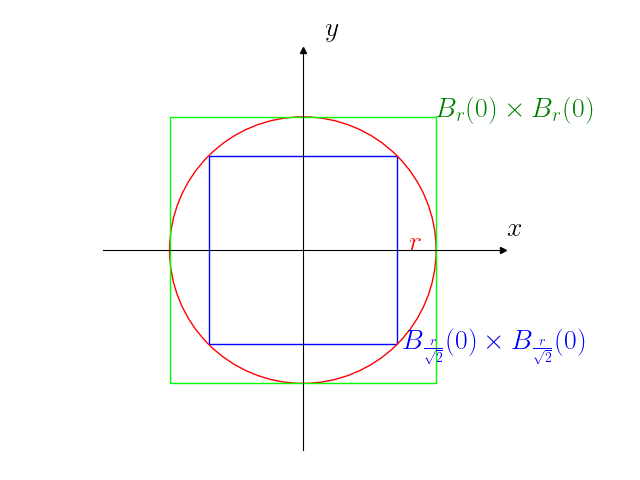
\includegraphics[width=0.7\linewidth]{spazi_metrici_e_normati/pag175}
			\label{fig:pag175}
		\end{center}
			
		\item Sia ora $Y = \mathbb{R}$ con la metrica usuale che deriva dal valore assoluto.
		
		$f:X \rightarrow \mathbb{R}$
		
		$A = \{ (x,y) \in X \times \mathbb{R} \; \big| \; y > f(x) \}$
		
		$C = \{ (x,y) \in X \times \mathbb{R} \; \big| \; y \geq f(x) \}$
		
		Provare che, se $f $ è continua, allora $A$ è aperto e $C$ è chiuso in $X \times \mathbb{R}$ con la metrica $d$.
		
		\item Provare che, in generale, il viceversa non è vero, cioè $A$ può essere aperto con $f$ discontinua e $C$ chiuso con $f$ discontinua.	
	\end{enumerate}
	
	\hline
	
	\begin{enumerate}
		\item Per casa
		
		\item Facciamo vedere che se $(x,y) \in B_{\frac{r}{\sqrt{2}}}^{X}(x_0) \times B_{\frac{r}{\sqrt{2}}}^{Y}(y_0)$, allora $(x, y) \in B_{r}^{X \times Y} ((x_0, y_0))$
		
		\begin{equation*}
			d_x(x, x_0) < \frac{r}{\sqrt{2}} \text{  e  } d_y(y, y_0) < \frac{r}{\sqrt{2}}
			\Rightarrow d((x,y), (x_0,y_0)) < r
		\end{equation*}
		\begin{align*}
			d((x,y),(x_0,y_0)) 
			&= \sqrt{(d_x(x, x_0))^2 + (d_y(y,y_0))^2} <
			\\
			&< \sqrt{\left( \frac{r}{\sqrt{2}} \right)^2+\left( \frac{r}{\sqrt{2}} \right)^2} = \sqrt{r^2} = r
		\end{align*}

		Facciamo vedere che, se $(x,y) \in B_{r}^{X \times Y}((x_0, y_0))$, allora $(x,y) \in B_{r}^{X} (x_0) \times B_{r}^{Y} (y_0)$, cioè che, se $d((x,y), (x_0,y_0)) < r$, allora $d_x(x, x_0) < r$ e $d_y(y, y_0) < r$
		
		\begin{equation*}
			d_x (x, x_0)= \sqrt{(d_x (x, x_0))^2} \leq \sqrt{(d_x (x, x_0))^2 + (d_y (y, y_0))^2} = d((x,y), (x_0,y_0)) < r
		\end{equation*}
	
		\item Introduciamo la funzione 
		\begin{align*}
			\phi: 
			&X \times \uppercomment{\mathbb{R}} {} {\text{c'è la metrica } d} \rightarrow \mathbb{R},
			\\
			&(x,y) \mapsto y-f(x)
		\end{align*}
		\begin{gather*}
			A= \{ (x,y) \in X \times \mathbb{R} \; \big| \; \phi(x, y) > 0 \} = \phi^{-1} \big( ]0,+\infty[ \big)
			\\
			C = \{ (x,y) \in X \times \mathbb{R} \; \big| \; \phi(x, y) \geq 0 \} = \phi^{-1} \big( ]0,+\infty[ \big)
			\\
			\phi^{-1} \big( B^c \big) = \big( \phi^{-1}(B) \big)^c
			\\
			x \in \phi^{-1} \big( B^c \big) \iff \phi(x) \in B^c \iff \phi(x) \notin B \iff x \notin \phi^{-1} \big( B \big) \iff x \in \big( \phi^{-1}(B) \big)^c
		\end{gather*}

		Se $B$ è chiuso e $\phi$ è continua, 
		\begin{gather*}
			\phi^{-1} \big( B \big) = \phi^{-1}\big( (B^c)^c\big) =
			\\
			= \big( \lowercomment{\phi^{-1} (\lowercomment{B^c} {\text{aperto}} {}) } {\text{aperto}} {} \big)^c \text{ è chiuso}
		\end{gather*} 
		
		cioè l'antimmagine di un chiuso tramite una funzione continua è un insieme chiuso.
		
		Poiché $B = [0,+\infty[$ è chiuso e $C = \phi^{-1} \big( B \big)$, se $\phi$ è continua, $C$ è chiuso.
		
		Tutto l'esercizio si riduce a dimostrare che $\phi$ è continua.
		
		\begin{align*}
			\phi_1: 
			& X \times \mathbb{R} \rightarrow \mathbb{R},
			& \phi_2: 
			& X \times \mathbb{R} \rightarrow \mathbb{R}
			\\
			& (x,y) \mapsto y
			&
			& (x,y) \mapsto f(x)
		\end{align*}
		\begin{equation*}
			\phi(x,y) = \phi_1(x,y) - \phi_2(x,y)
		\end{equation*}
		
		Se dimostro che $\phi_1$ e $\phi_2$ sono continue, allora $\phi$ è continua perché differenza di funzioni continue.
		
		Dimostriamo la continuità di $\phi_1$.
		
		$(x_0, y_0) \in X \times \mathbb{R}$ e fissiamo $\epsilon > 0$
		
		Dobbiamo dimostrare che $\exists \ \delta > 0 \; \big| \; \text{ se } d((x,y), (x_0,y_0)) < \delta$, allora $\lowercomment{|y-y_0|}{| \phi_1(x, y) - \phi_2 (x_0, y_0) |}{} < \epsilon$
		
		Sia $U = X \times  ]y_0 - \epsilon, y_0 + \epsilon[$
		
		Se $(x,y) \in U \Rightarrow |\phi_1(x,y) - \phi_1(x_0,y_0)| = |y - y_0| < \epsilon$
		
		$U$ è un intorno di $(x_0, y_0)$, cioè
		\begin{gather*}
			\exists \ \delta > 0 \; \big| \; B_{\delta}^{X \times \mathbb{R}} ((x_0, y_0)) \subseteq U
			\\
			B_{\delta}^{X \times \mathbb{R}} ((x_0, y_0))\subseteq B_{\delta}^{X} (x_0) \times B_{\delta}^{\mathbb{R}} (y_0) \subseteq X \times ]y_0 - \epsilon, y_0 + \epsilon[
		\end{gather*}

		Continuità di $\phi_2$ in $(x_0,y_0)$
		
		$\forall \ \epsilon > 0$ devo trovare $\delta >0 \; | \; \text{ se } d((x,y), (x_0,y_0)) < \delta$ 
		\begin{equation*}
			\Rightarrow | \phi_2(x,y) - \phi_2(x_0,y_0)| = |f(x) - f(x_0)| < \epsilon
		\end{equation*}

		Poiché $f$ è continua, $\exists \ \delta > 0 \; \big| \; x \in B_{\delta}^{X} (x_0) \Rightarrow |f(x) - f(x_0)| < \epsilon$
		
		L'insieme $B_{\delta}^{X} (x_0) \times \mathbb{R}$ è un intorno di $(x_0,y_0)$ e $\forall \ (x,y) \in B_{\delta}^{X} (x_0) \times \mathbb{R}$ si ha
		\begin{equation*}
			|\phi_2(x,y) - \phi(x_0,y_0)| = |f(x) - f(x_0)| < \epsilon
		\end{equation*}
		
		\item $X = Y = \mathbb{R}$ con la distanza data dal valore assoluto
		
		\begin{equation*}
			f(x) = \lowercomment{\chi_{[0,+\infty[}(x)} {\text{funzione caratteristica di }[0,+\infty[}{\text{o funzione di Heaviside}} =
			\begin{cases}
				1 & \text{se } x \geq 0
				\\
				0 &  \text{se } x < 0
			\end{cases}
		\end{equation*}
		
		\begin{center}
			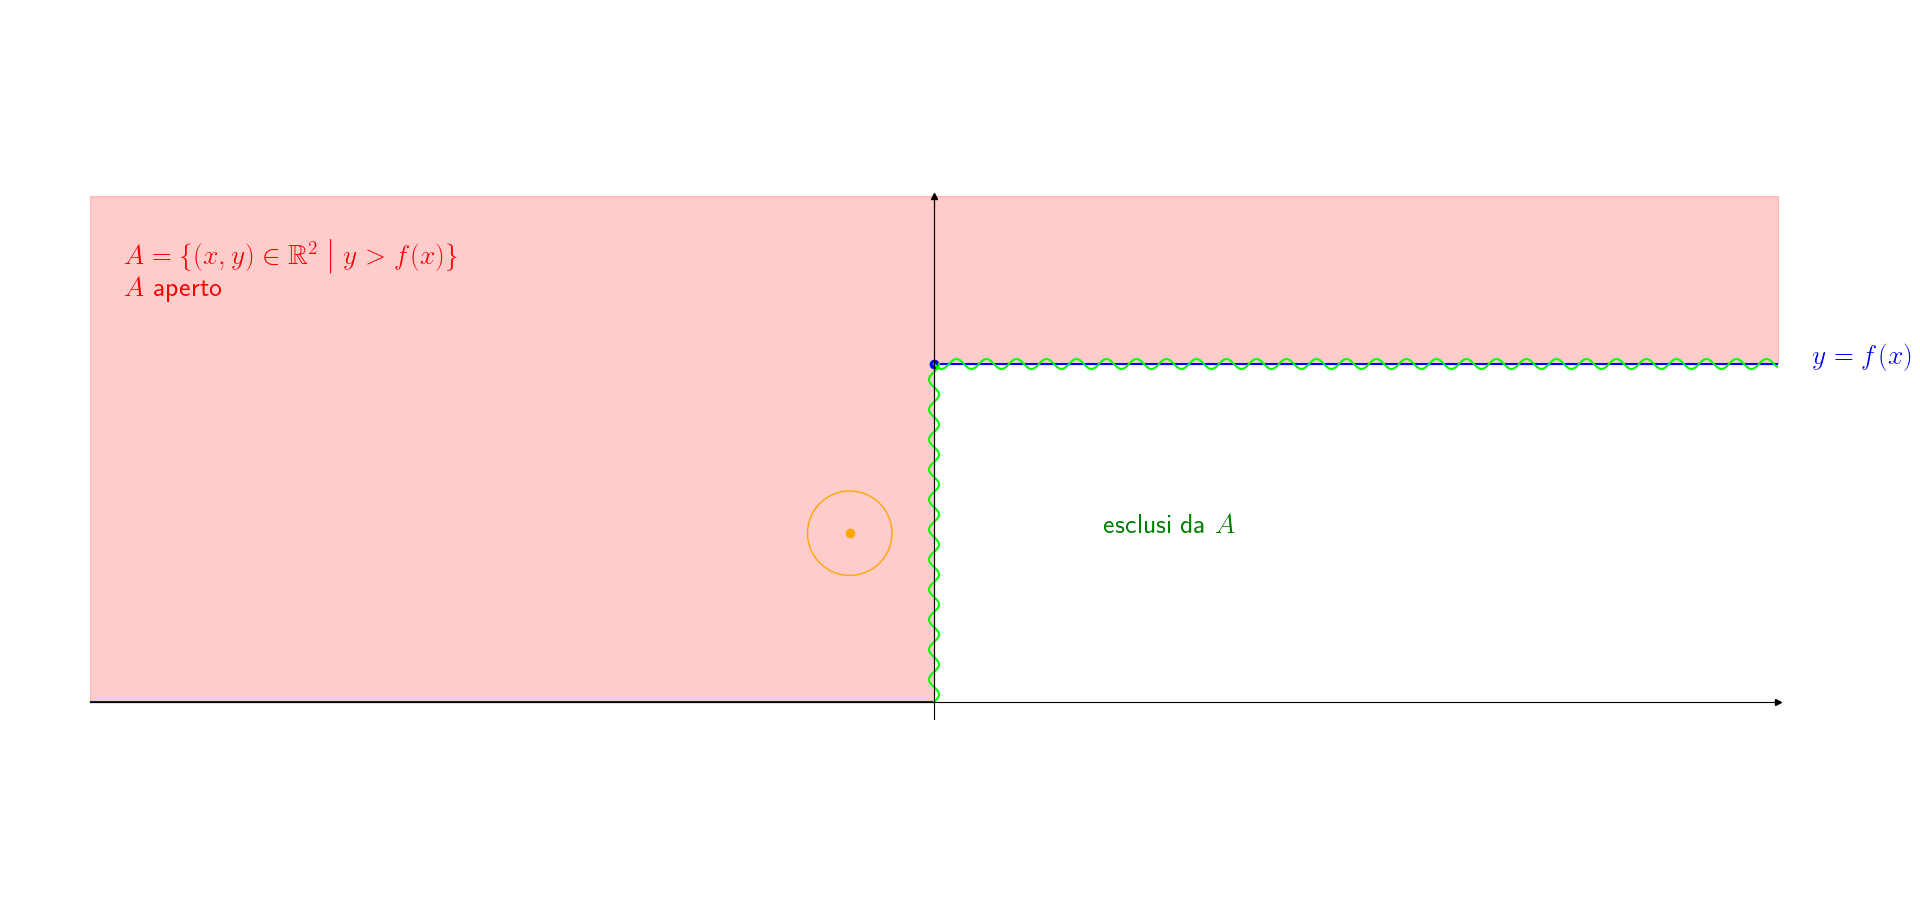
\includegraphics[width=0.7\linewidth]{spazi_metrici_e_normati/pag181_1}
			\label{fig:pag1811}
		\end{center}
		
		\begin{equation*}
			f(x) = 		\chi_{]0,+\infty[} = 
			\begin{cases}
				1 & \text{se } x > 0
				\\
				0 &  \text{se } x \leq 0
			\end{cases}
		\end{equation*}
		
		\begin{center}
			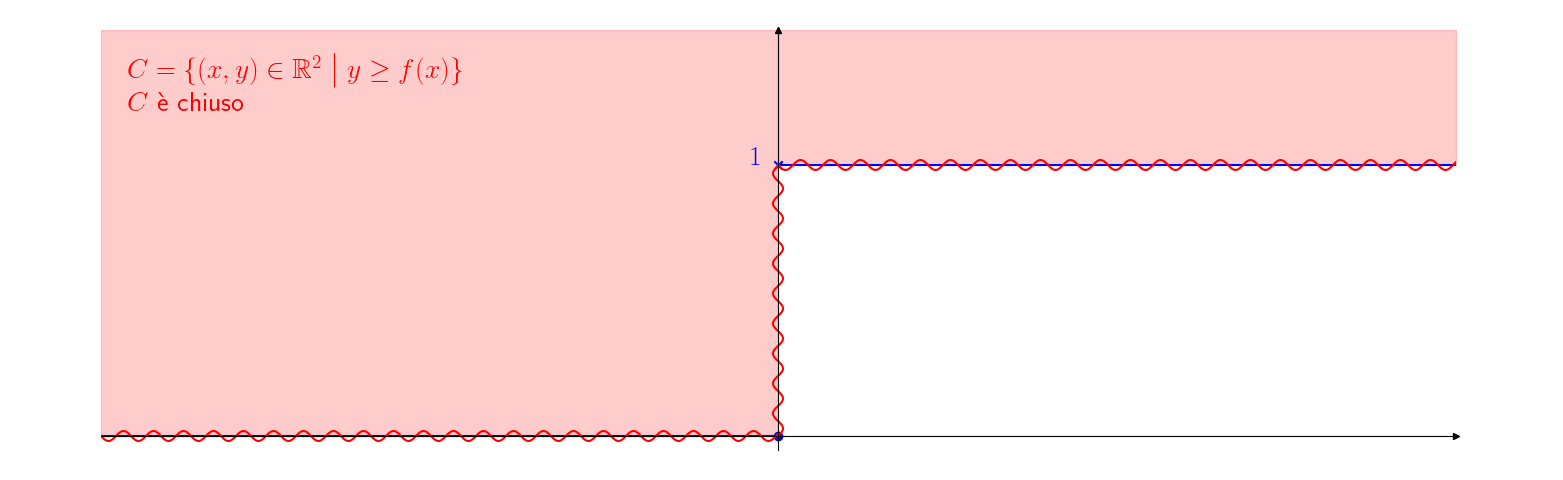
\includegraphics[width=0.7\linewidth]{spazi_metrici_e_normati/pag181_2}
			\label{fig:pag1812}
		\end{center}
	\end{enumerate}
\end{example}
\end{exbar}


\subsection{Successioni di funzioni}

\begin{definition}
	$(X,d)$ spazio metrico.
	
	Una successione di funzioni da $X$ in $\mathbb{R}$ è una funzione che ad ogni numero naturale $k$ associa una ed una sola funzione $f_k : X \rightarrow \mathbb{R}$. 
\end{definition}


\begin{definition}
	Sia $\{ f_k \}_{k \in \mathbb{N}}, f_k : X \rightarrow \mathbb{R}$, successione di funzioni. Si dice che la successione \textbf{converge puntualmente} in $D \subseteq X$ se $\{ f_k(x) \}_{k \in \mathbb{N}}$ converge $\forall \ x \in D$, cioè se $\forall \ x \in D$ esiste finito
	\begin{equation*}
		\lim_{k \rightarrow + \infty} f_k(x) = f(x),
	\end{equation*}
	limite puntuale della successione $f : D \rightarrow \mathbb{R}$. L'insieme degli $x \in X$ dove $\{f_k \}_{k \in \mathbb{N}}$ converge puntualmente si dice \textbf{insieme di convergenza puntuale} della successione.
\end{definition}


\begin{exbar}
	\begin{gather*}
	f_k: \mathbb{R} \rightarrow \mathbb{R}, \qquad f_k(x) = x^k
	\\
	\lim_{k \rightarrow + \infty} f_k(x) = \lim_{k \rightarrow + \infty} x^k =
	\begin{cases}
		0 & \text{se } |x|<1
		\\
		1 & \text{se } x=1 
		\\
		\nexists & \text{se } x \leq -1
		\\
		+\infty & \text{se } x >1
	\end{cases}
	\end{gather*}
	
	Insieme di convergenza puntuale: $D = ]-1,1]$
	
	Limite puntuale $f:D \rightarrow \mathbb{R}$		
	\begin{equation*} f(x) = \begin{cases}
		0 & \text{se } |x|<1
		\\
		1 & \text{se } x=1
	\end{cases}
	\end{equation*}	
\end{exbar}


\begin{definition}
	$f_k:X \rightarrow \mathbb{R}, k \in \mathbb{N}$, successione di funzione. Si dice che $\{ f_k \}_{k \in \mathbb{N} }$ \textbf{converge uniformemente} in $D \subseteq X$ ad una funzione $f: D \rightarrow \mathbb{R}$ se 
	\begin{gather*}
		\lim_{k \rightarrow +\infty} \sup_{x \in D} |f_k(x) - f(x)| = 0 
		\\
		\text{e si scrive } f_k \rightrightarrows f \text{ in } D
	\end{gather*}
	
	($\forall \epsilon >0 \exists N \; \big| \; k >N \qquad \sup_{x \in D} |f_k(x)-f(x)| < \epsilon$, e quindi, in particolare $|f_k(x) - f(x)| < \epsilon  \quad \forall \ x \in D$ cioè $f(x) - \epsilon <f_k(x) < f(x) + \epsilon \qquad \forall x \in D$)
	
	\begin{center}
		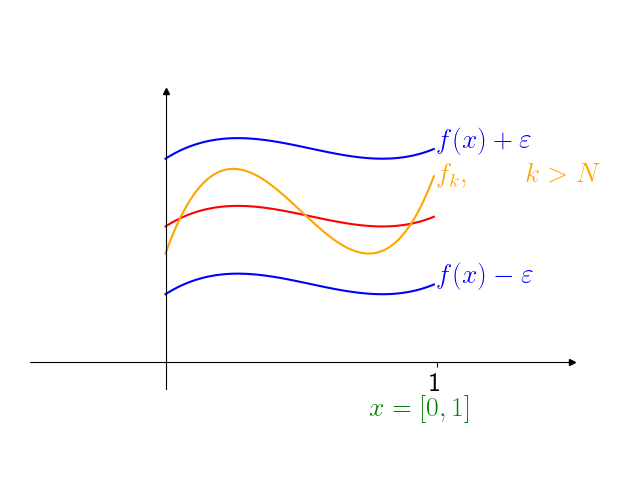
\includegraphics[width=0.7\linewidth]{spazi_metrici_e_normati/pag184}
		\label{fig:pag184}
	\end{center}
\end{definition}


\begin{exbar}
	$(X,d)$ spazio metrico
	
	$B(x) = \{ f:X \rightarrow \mathbb{R} \; \big| \; \lowercomment{f \text{ è limitata }} {\exists \ M > 0 \; | \; |f(x)| \leq M} {\forall x \in X} \} $ 
	
	$f\in B(x)$
	\begin{equation*}
		\parallel f \parallel_\infty = \sup_{x \in X} |f(x)|\text{, norma infinito di } f
	\end{equation*}
	$f_k \rightrightarrows f$ in $X$ se $\parallel f_k - f \parallel_\infty \rightarrow 0$ per $k \rightarrow +\infty$
	
	cioè la convergenza uniforme è la convergenza per $\parallel \cdot \parallel_\infty$.
\end{exbar}


\begin{proposition}
	\label{pr: pag185}
	Se $f_k \rightrightarrows f$ in $D$, allora $\{ f_k \}_{k \in \mathbb{N}}$ converge puntualmente ad $f$ in $D$.
\end{proposition}


\begin{dembar}
	\textbf{Dimostrazione} della \textbf{Proposizione \ref{pr: pag185}}
	
	Se $x \in D$
	\begin{gather*}
		0 \leq |f_k(x) - f(x)| \leq \underbrace{\sup_{y\in D}|f_k(y)-f(y)|}_{0 \text{ per } k \to +\infty} 
		\\
		\Rightarrow |f_k(x) - f(x)| \rightarrow 0 \text{ per } k \rightarrow +\infty
		\\
		\text{cioè } f(x) = \lim_{k \rightarrow +\infty f_k (x)} \qquad \forall \ x \in D.
	\end{gather*}
\end{dembar}


\begin{exbar}
\begin{example}
	\begin{equation*}
		f_k(x) = x^k, \qquad x \in \mathbb{R}
	\end{equation*}

	Insieme di convergenza puntuale è $D=]-1,1]$
	
	Limite puntuale $f:D \rightarrow \mathbb{R}$
	\begin{equation*}
		f (x) = 
		\begin{cases}
			0 & \text{se } -1 < x < 1
			\\
			1 & \text{se } x = 1
		\end{cases}
	\end{equation*}
	
	$f_k \rightrightarrows f$ in $D$?

	\begin{gather*}
		\rho_k(x)= \frac{e^{-x^2}}{k}, \qquad x \geq 1, \quad x \in \mathbb{R}
		\\
		\lim_{k \rightarrow +\infty} g_k(x)=0 \qquad \forall x
	\end{gather*}

		$\{ \rho(x) \}_{k \geq 1}$ converge puntualmente alla funzione nulla $\rho(x) = 0 \qquad  \forall x \in \mathbb{R}$ in $\mathbb{R}$
		\begin{gather*}
			\sup_{x \in \mathbb{R}} |\rho_k(x) - \rho(x)| = \sup_{x \in \mathbb{R}} \frac{e^{-x^2}}{k} = \frac{1}{k} \rightarrow 0
			\\
			\rho_k \rightrightarrows g \text{ in } \mathbb{R}
		\end{gather*}

	\begin{gather*}
		\phi_k(x) = \frac{x^2}{k}, \qquad k \geq 1, \quad x \in \mathbb{R}
		\\
		\lim_{k \rightarrow +\infty} \phi_k(x) = 0 = \phi(x) \qquad \forall x \in \mathbb{R}
	\end{gather*}
	
	Insieme di convergenza puntuale è $\mathbb{R}$ e il limite puntuale è la funzione nulla
	
	\begin{gather*}
		\sup_{x \in \mathbb{R}} |\phi_k(x) - \phi(x)| = \sup_{x \in \mathbb{R}} \frac{x^2}{k} = +\infty
		\\
		\phi_k \nrightrightarrows \phi \text{ in } \mathbb{R}
	\end{gather*}
		
	Fissato $M > 0$, ho convergenza uniforme in $[-M, M]$?
	
	\begin{gather*}
		\sup_{x \in [-M,M]} |\phi_k(x) - \phi(x)| = \sup_{x \in [-M,M]} \frac{x^2}{k} = \frac{M^2}{k} \rightarrow 0 \text{ per } k \rightarrow + \infty
		\\
		\phi_k \rightrightarrows \phi \text{ in } [-M, M] \qquad \forall \ M > 0 \
		\text{\textcolor{red}{ ma non in $\mathbb{R}$}.}
	\end{gather*}
	
	Torniamo a $f_k =x^k$
	
	\begin{gather*}
		\sup_{x \in ]-1, 1]} |f_k(x) - f(x)| \geq \sup_{x \in ]-1, 1[} |f_k(x) - f(x)| = \sup_{x \in ]-1, 1[} |x^k| = 1 \qquad \forall \ k
		\\
		f_k \nrightrightarrows f \text{ in } ]-1, 1]
	\end{gather*}
	
	Sia $0 < \epsilon < 1$ e studiamo la convergenza uniforme in $[-1+\epsilon, 1-\epsilon]$
	\begin{gather*}
		\sup_{x \in [-1+\epsilon, 1-\epsilon]} |f_k(x) - f(x)| = \sup_{x \in [-1+\epsilon, 1-\epsilon]} |f_k(x)| = \sup_{x \in [-1+\epsilon, 1-\epsilon]} |x^k| =
		\\
		= (1-\epsilon)^k \rightarrow 0 \text{ per } k \rightarrow +\infty \text{ perché } 0 < 1 - \epsilon < 1 
		\\
		\Rightarrow f_k \rightrightarrows f \text{ in } [-1+\epsilon, 1-\epsilon] \qquad  \forall \epsilon > 0 \ \text{\textcolor{red}{ ma non in $]-1,1]$!}}
	\end{gather*}
\end{example}
\end{exbar}


\begin{exbar}
\begin{example}
	\begin{equation*}
		f_k(x) = \frac{kx}{1+k|x|}, \qquad k \geq 0, \quad x \in \mathbb{R}
	\end{equation*}
	
	Convergenza puntuale
	\begin{equation*}
		\lim_{k \rightarrow +\infty} f_k(x) = \begin{cases}
			1 & \text{se } x > 0 
			\\
			0 & \text{se } x = 0 
			\\
			-1 & \text{se } x < 0
		\end{cases}
	\end{equation*}
		
		L'insieme di convergenza puntuale è $\mathbb{R}$ e il limite puntuale è la funzione segno
		\begin{gather*}
			sgn(x) = 
			\begin{cases}
				1 & \text{se } x > 0
				\\
				0 & \text{se }  x = 0
				\\
				-1 & \text{se }  x < 0
			\end{cases}
			\\
			\sup_{x \in \mathbb{R}} |f_k(x) - sgn(x)| \geq \sup_{x>0} |f_k(x) - sgn(x)| =
			\\
			= \sup_{x>0} |\frac{kx}{1+kx} - 1| = \sup_{x>0} |\frac{1}{1+kx}| = 1
			\\
			f_k \nrightrightarrows sgn\text{ in } \mathbb{R}
	\end{gather*}
	
	Fissiamo $\epsilon > 0$ e studiamo la convergenza uniforme in $]-\infty - \epsilon] \cup [\epsilon, +\infty[$
	
	\begin{align*}
		\sup_{|x| \geq \epsilon} |f_k(x) - sgn(x)| 
		&\uppercomment{=}{f_k \text{ e } sgn}{\text{sono dispari}} 
		\sup_{x \geq \epsilon} |f_k(x) - sgn(x)| 
		\\
		&= \sup_{x \geq \epsilon} |\frac{1}{1+kx}|= \frac{1}{1+k\epsilon} \rightarrow 0 \text{ per } k \rightarrow +\infty
	\end{align*}
	\begin{gather*}
		f_k \rightrightarrows sgn \text{ in } ]-\infty, -\epsilon] \cup [\epsilon, +\infty[ \qquad \forall \epsilon > 0, \text{\textcolor{red}{ma non in $\mathbb{R} \backslash \{ 0 \}$}}
		\\
		\sup_{x \in \mathbb{R} \backslash \{ 0 \}} |f_k(x) - sgn(x)| \uppercomment{=} {} {\text{per simmetria}} \sup_{x >0} |f_k(x) - sgn(x)| = 1 \qquad \forall k
	\end{gather*}
\end{example}
\end{exbar}
	
	
\begin{theorem}
	\label{th: pag190}
	$(X,d)$ spazio metrico, $f_k:X \rightarrow \mathbb{R}$, $\{f_k\}_{k \in \mathbb{N}}$ successione di funzioni tale che $f_k \rightrightarrows f$ in $D$. 
	
	Se $f_k$ è continua in $x_0 \in X \quad \forall \ k \in \mathbb{N}$, allora $f$ è continua in $x_0$. In particolare, se $f_k \in C^0(X) \quad \forall \ k \in \mathbb{N}$, allora $f \in C^0(X)$
	
	(il limite uniforme di funzioni continue è continuo.)
\end{theorem}


\begin{attbar}
	\textbf{Osservazione:}
	
	$f_k(x) = \frac{kx}{1+k|x|}$ non può convergere uniformemente a $sgn$ in $\mathbb{R}$ perché $f_k \in C^0 (\mathbb{R}) \quad  \forall \ k$, ma $sgn$ ha un punto di salto in $x=0$.
\end{attbar}


\begin{dembar}
	\textbf{Dimostrazione} del \textbf{Teorema \ref{th: pag190}}
	
	
	$x_0 \in X$. Fissiamo $\epsilon > 0$. Dobbiamo dimostrare che $\exists \ \delta > 0 \; \big| \; d(x,x_0) < \delta \Rightarrow |f(x) - f(x_0)| < \epsilon$
	\begin{itemize}
		\item $f_k$ è continua in $x_0 \quad \forall \ k$
		\item $f_k \rightrightarrows f$ in $X$
	\end{itemize}
	\begin{gather*}
		f_k \rightrightarrows f \text{ in } X \Rightarrow \exists \ N > 0 \; \big| \ k > N \Rightarrow |f_k(x) - f(x)| < \frac{\epsilon}{3} \qquad \forall \ x \in X
		\\
		\text{perché } \sup_{x \in X}|f_k(x) - f(x)| < \frac{\epsilon}{3}
	\end{gather*}

	Fissiamo $\overline{k} > N$, cosicché $|f_{\overline{k}}(x) - f(x)| < \frac{\epsilon}{3} \quad \forall \ x \in X$ e sia $\delta > 0 \; \big| \;  d(x,x_0) < \delta$
	\begin{equation*}
		\Rightarrow |f_{\overline{k}}(x) - f_{\overline{k}}(x_0)| < \frac{\epsilon}{3}
	\end{equation*} 
	
	($\delta$ esiste perché $f_{\overline{k}}$ è continua in $x_0$).
	\begin{align*}
		|f(x) - f(x_0)| 
		& =|(f(x) - f_{\overline{k}}(x)) + (f_{\overline{k}}(x) - f_{\overline{k}}(x_0)) + (f_{\overline{k}}(x_0) - f(x_0))| \leq
		\\
		& \leq  \uppercomment{|f(x) - f_{\overline{k}}(x)|}
		{}{<\frac{\epsilon}{3} \text{ per } \overline{k} > n} 
		+ \uppercomment{|f_{\overline{k}}(x) - f_{\overline{k}}(x_0)|}
		{}{<\frac{\epsilon}{3} \text{ se } d(x, x_0) < \delta} 
		+ 
		\uppercomment{|f_{\overline{k}}(x_0) - f(x_0)|}
		{}{<\frac{\epsilon}{3} \text{ per } \overline{k} > n} 
		<
		\\
		& < \frac{\epsilon}{3} + \frac{\epsilon}{3} + \frac{\epsilon}{3} = \epsilon \text{ a patto che } d(x,x_0)< \delta \qquad \square
	\end{align*}
\end{dembar}


\begin{attbar}
	Tutto quello che abbiamo detto e che diremo  per successioni di funzioni a valori in $\mathbb{R}$ vale per successioni di funzioni a valori in $\mathbb{C}$.
\end{attbar}


\begin{exbar}
\begin{example}
	\begin{gather*}
		\phi: [0,1] \rightarrow \mathbb{R}^{\geq 0} \text{ continua}
		\\
		C = \{ f \in C^\circ ([0,1]) \; \big| \; |f(x)| \leq \phi(x) \forall x \in [0,1] \}
	\end{gather*}

	Dotato $C^0 ([0,1])$ con la norma $\parallel \cdot \parallel_\infty$, provare che $C$ è chiuso e trovare $\partial C$.
	\begin{itemize}
		\item $C$ è chiuso $\iff$ presa $\{f_k\}_{k \in \mathbb{N}} \subseteq C$, convergente per $\parallel \cdot \parallel_\infty$ a $f:[0,1] \rightarrow \mathbb{R}$, si ha che $f \in C$.
		
		$\{ f_k \}_{k \in \mathbb{N}} \subseteq C, \quad f_k \rightrightarrows f \Rightarrow f \in C^0([0,1])$ perché limite uniforme di una successione di funzioni continue. Affinché $f \in C$, deve essere $|f(x)| \leq \phi(x) \quad \forall x \in [0,1]$
		
		Sappiamo che $\forall x \in [0,1] \quad |f_k(x)| \leq \phi(x) \quad \forall k \in \mathbb{N}$ perché $f_k \in C \quad \forall k \in \mathbb{N}$
		
		$f_k \rightrightarrows f$ in $[0,1] \Rightarrow f_k(x) \rightarrow f(x) \quad \forall x \in [0,1] $ perché la convergenza uniforme implica quella puntuale 
		\begin{gather*}
			\Rightarrow |f_k(x)| \rightarrow |f(x)| \qquad \forall x \in [0,1]
			\\
			|f_k(x)| \leq \phi(x) \qquad \forall x \in [0,1]
			\\
			\color{blue}{ \tiny{\downarrow \text{ passando al limite per } k \to +\infty } } 
			\\
			\Rightarrow |f(x)| \leq \phi(x) \qquad \forall x \in [0,1]
			\\
			\Rightarrow f \in C \Rightarrow C \text{ è chiuso}
		\end{gather*}

		\item Troviamo $\partial C$
		\begin{align*}
			C 
			&= \{ f \in C^0 ([0,1]) \; \big| \; |f(x)| \leq \phi(x) \qquad \forall x \in [0,1] \} 
			\\
			&= \{ f \in C^0 ([0,1]) \; \big| \; -\phi(x) \leq f(x) \leq \phi(x) \qquad \forall x \in [0,1] \}
		\end{align*}

		\segnaposto %194
		\begin{equation*}
			f_0 \in \partial C \Leftrightarrow \forall \epsilon > 0, B_\epsilon(f_0) \cap C \neq \emptyset \text{ e } B_\epsilon (f_0)\cap C^c \neq \emptyset
		\end{equation*}

		
		Congettura: 
		\begin{equation*}
			\partial C = \{ f \in C^0 ([0,1]) \; \big| \; \exists x_0 \in [0,1] \; \big| \; |f(x_0)| = \phi(x_0) \}
		\end{equation*}
		
		Sia $f\in \partial C$ e proviamo che $\exists x_0 \in [0,1] \; \big| \; |f(x_0)| = \phi(x_0)$
		
		$f \in \partial C \Rightarrow f \in C$ perché $C$ è chiuso $\Rightarrow |f(x)| \leq \phi(x) \quad \forall x \in [0,1]$.
		
		Per assurdo, assumiamo che 
		\begin{equation*}
			|f(x)| < \phi(x)  \qquad \forall x \in [0,1]
		\end{equation*}
		
		E' vero o falso che $\inf_{x \in [0,1]}( \phi(x) -|f(x)| )>0$?	
		\segnaposto %195
		
		$[0,1]$ è compatto quindi $\phi - |f|$ è continua 
		\begin{align*}
			\Rightarrow \inf_{x \in [0,1]} [\phi(x) - |f(x)|] 
			&= \min_{x \in [0,1]} [\phi(x) - |f(x)|] =
			\\
			&= \phi(x_0) - |f(x_0) > 0 \qquad \exists x_0 \in [0,1]
			\\
			&= r
		\end{align*}
		
		$\Rightarrow B_{\frac{r}{2}}(f) \leq C$ perché, fissata $\rho \in B_{\frac{r}{2}}(f)$ si ha
		
		\begin{align*}
			|\rho(x)| 
			&\leq |g(x) - f(x) + f(x)| 
			\\
			&\leq |g(x) - f(x)| + |f(x)| \lowercomment{<} {\text{perché} \parallel \rho - f \parallel_\infty < \frac{r}{2}} {} \frac{r}{2} + |f(x)| 
			\\
			&\lowercomment{\leq} 
			{\phi(x) - |f(x)| \geq r > 0 \quad \forall x \in [0, 1]} 
			{|f(x)| \leq \phi(x) -r \qquad \forall x \in [0, 1] }
			\frac{r}{2} + \phi(x) - r = \phi(x) - \frac{r}{2} \\
			&\leq \phi(x) \qquad \forall x \in [0,1]
		\end{align*}
		\begin{equation*}
			\Rightarrow \rho \in C \Rightarrow B_{\frac{r}{2}}(f) \cap C^c = \emptyset \Rightarrow f \notin \partial C \text{, assurdo.}
		\end{equation*}

		Adesso proviamo che, se $\uppercomment{f \in C} {C \text{ chiuso}} {\partial C \subseteq C}$ è tale che $\exists x_0 \in [0,1] \; \big| \; |f(x_0)| = \phi(x_0)$, allora $f \in \partial C$, cioè $\forall \ \epsilon > 0$, $B_\epsilon(f) \cap C \neq \emptyset$ e $B_\epsilon(f) \cap C^c \neq \emptyset$.
		
		Sicuramente $f \in B_\epsilon (f) \cap C$, che così è diverso da $\emptyset$.
		
		Basta verificare che $\forall \ \epsilon > 0$, $B_\epsilon (f) \cap C^c \neq \emptyset$
		
		$|f(x_0|=\phi(x_0)$. Per fissare le idee assumiamo che $f(x_0)\geq 0$
		\begin{equation*}
			f(x_0) = |f(x_0)|= \phi(x_0)
		\end{equation*}

		\segnaposto %196
		\begin{gather*}
			\epsilon >0, \qquad f + \frac{\epsilon}{2} = \rho, \qquad  |g(x_0)| = f(x_0) + \frac{\epsilon}{2} > \phi(x_0)
			\\
			g \notin C \text{ e } \parallel g - f \parallel_\infty = \frac{\epsilon}{2} < \epsilon
			\\
			g \in B_\epsilon (f) \Rightarrow B_\epsilon (f) \cap C^c \neq \emptyset\text{, come si voleva.}
		\end{gather*}	
	\end{itemize}
\end{example}
\end{exbar}


\begin{exbar}
\begin{example}
	Data la successione di funzioni
	\begin{equation*}
		f_k: \mathbb{R} \backslash \{0\} \rightarrow \mathbb{R}, \qquad k \geq 1
	\end{equation*}
	
	definita da
	\begin{equation*}
		f_k(x) = \frac{\ln x^{2k}}{(1 + x)^{2k}}
	\end{equation*}
	
	trovare gli insiemi di convergenza puntuale e uniforme.
	\begin{align*}
		\lim_{k \rightarrow +\infty} f_k(x) = \lim_{k \rightarrow +\infty} 2k \frac{\ln |x|}{(1+x)^{2k}}
		&=\begin{cases}
			+\infty & \text{se } |1 + x| \leq 1 \text{ e } |x| > 1 
			\\
			-\infty & \text{se } |1 + x| \leq 1 \text{ e } |x| < 1
			\\
			0 & \text{se } |1 + x| \geq 1
		\end{cases}
		\\
		&=\begin{cases}
			+\infty & \text{se } -2 \leq x <- 1 
			\\
			-\infty & \text{se } -1 < x < 0 
			\\
			0 & \text{se } x < -2 \text{ o } x > 0
		\end{cases}
	\end{align*}
	
	L'insieme di convergenza puntuale è $D = ]-\infty,-2[ \cup ]0,+\infty[$ e il limite puntuale è la funzione $f(x) = 0 \quad \forall x \in D$.
	
	Studiamo la convergenza uniforme in $D$ e studiamo separatamente gli intervalli $]-\infty,-2[$ e $]0,+\infty[$.
	
	Valutiamo 
	\begin{align*}
		\sup_{x >0} |f_k(x) - f(x)|
		&\uppercomment{=}{}{k \text{ fissato!}}
		\sup_{x >0}|f_k (x)| = \sup_{x>0}2k \frac{|\ln |x||}{(1+x)^{2k}} 
		\geq \lim_{x \rightarrow 0^+} \frac{2k |\ln|x||}{(1+x)^{2k}} = +\infty
	\end{align*}
	\begin{equation*}
		f_k \nrightrightarrows f \text{ in } ]0,+\infty[
	\end{equation*}
	
	Vediamo cosa succede in $]-\infty,-2[$
	\begin{align*}
		\sup_{x < -2}|f_k(x) - f(x)| 
		&= \sup_{x<-2} |f_k(x)| = \sup_{x <-2}2k \frac{|\ln|x||}{|1+x|^{2k}}
		&\geq\lim_{x \rightarrow -2^-} \frac{2k|\ln |x|}{|1+x|^{2k}}= 2k \ln 2 \xrightarrow{k \rightarrow +\infty} +\infty 
	\end{align*}
	\begin{equation*}
		f_k \nrightrightarrows f \text{ in } ]-\infty,-2[
	\end{equation*}

	Proviamo a studiare la convergenza uniforme in sottointervalli di $]0,+\infty[$ e $]-\infty,-2[$.
	
	Concentriamoci su $]0,+\infty[$ e studiamo l'andamento di $f_k$ in questo intervallo
	\begin{gather*}
		f_k(x) = 2k \frac{\ln |x|}{(1+x)^{2k}} \qquad x >0
		\\
		\lim_{x \rightarrow 0^+} f_k(x) = -\infty \qquad \lim_{x \rightarrow +\infty} f_k(x) = 0
		\\
		f_k' (x) = 2k \frac{1+x(1-2k \ln |x|)}{x(1+x)^{2k+1}}
		\\
		f_k' (x) \geq 0 \iff 1+x(1-2k \ln |x|) \geq 0, \qquad x >0
	\end{gather*}

	se $x \in ]0,1]$, $-\ln x \geq 0$
	\begin{gather*}
		\Rightarrow 1+x(1-2k\ln x)\geq 0
		\\
		\lim_{x \rightarrow +\infty} [1+x(1-2k\ln x)]= -\infty
		\\
		\Rightarrow 1+x(1-2k\ln x)<0 \text{ definitivamente per } x \rightarrow +\infty
		\\
		f_k' (x) > 0 \qquad \forall x \in ]0,1] \text{ e } f_k' (x) < 0 \text{ definitivamente per } x \rightarrow +\infty
	\end{gather*} 
	
	\segnaposto %200
	Devo provare a vedere più in dettaglio il segno di $f_k' $, cioè di $\underbrace{1+x(1-2k \ln x)}_{\phi(x)}$, per $x \geq 1$
	\begin{gather*}
		\phi(1) = 2 > 0
		\\
		\phi'(x)=1-2k\ln x -2k = 1-2k(1+\ln x)< 0 \qquad \forall x >1
		\\
		\exists! \ \alpha_k > 1 \; \big| \; \phi(\alpha_k) = 0
	\end{gather*}
	\segnaposto %201_1
	$\exists! \ \alpha_k >1 \; \big| \; f_k' (\alpha_k)=0$
	
	\segnaposto %201_2
	\begin{align*}
		\sup_{x \geq a}|f_k (x)| 
		&= \max\{|f_k(a)|,|f_k(\alpha_k)|\}\leq
		\\
		&\leq |f_k(a)|+|f_k(\alpha_k)| = \lowercomment{2k \frac{|\ln a|}{(1+a)^{2k}}}
		{0 \text{ per } k \to +\infty} {}
		+ \lowercomment{|f_k(\alpha_k)|}{\text{da stimare}}{}
	\end{align*}
	\begin{gather*}
		f_k' (\alpha_k)=0
		\\
		1+\alpha_k (1-2k \ln \alpha_k)=0
		\\
		1+\alpha_k - 2 k \alpha_k \ln \alpha_k=0
		\\
		\ln\alpha_k= \frac{1+\alpha_k}{2k\alpha_k}
	\end{gather*}
	\begin{gather*}
		f_k (x)= 2k \frac{\ln x}{ (1+x)^{2k}}, \qquad x >0
		\\
		f_k(\alpha_k) = 2k\frac{\ln \alpha_k}{(1+\alpha_k)^{2k}} = 2k \frac{1+\alpha_k}{2k\alpha_k}\cdot \frac{1}{(1+\alpha_k)^{2k}} =
		\\
		= \frac{1}{\alpha_k(1+\alpha_k)^{2k-1}} \uppercomment{\leq} {} {k_\alpha > 1} \frac{1}{2^{2k-1}} \xrightarrow{k \rightarrow +\infty} 0 
		\\
		\sup_{x \geq a}|f_k(x)|\leq |f_k(a)|+|f_k(\alpha_k)|\xrightarrow{k \rightarrow +\infty} 0 \\
		\Rightarrow f_k \rightrightarrows f \text{ in } [a,+\infty[ \qquad \forall a >0
	\end{gather*}

	Studiamo $f_k$ in $]-\infty,-2[$.
	\begin{gather*}
		\lim_{x \rightarrow-2^-} f_k(x) = 2k\ln 2
		\\
		\lim_{x \rightarrow-\infty}f_k(x) = 0
		\\
		f_k' (x) = 2k \frac{1+x(1-2k\ln|x|)}{x(1+x)^{2k+1}}
	\end{gather*}

	Se $x <-2 $, $x(1+x)>0 \Rightarrow x(1+x)^{2k+1}>0$
	
	Se $x <-2$, $f_k'(x) \geq 0 \Leftrightarrow 1+x(1-2k\ln|x|)\geq 0$
	\begin{gather*}
		x <0 \text{ e } 1-2k\ln |x| \uppercomment{\leq} {} {x<-2} 1-2k \ln 2 < 0 \qquad \forall k \geq 1
		\\
		\Rightarrow x(1-2k\ln|x|)\geq 0 \qquad \forall x <-2
		\\
		\Rightarrow f_k'(x) > 0 \qquad \forall x \in ]-\infty,-2[
		\\
		\Rightarrow f_k \text{ è crescente in } ]-\infty,-2[ 
	\end{gather*}
	\segnaposto %204
	
	Fissato $b < -2$
	\begin{gather*}
		\sup_{x \leq b} |f_k(x)| = f_k(b)= 2k \frac{\ln |b|}{(1+b)^{2k}}\xrightarrow{k \rightarrow+\infty} 0
		\\
		\Rightarrow f_k \rightrightarrows f \text{ in } ]-\infty, b] \qquad \forall b < -2
		\\
		\Rightarrow f_k \rightrightarrows f \text{ in } ]-\infty,b] \cup [a, +\infty[ \qquad \forall b < -2 \text{ e } \forall a > 0
	\end{gather*}
\end{example}
\end{exbar}


\begin{attbar}
	$(X,d)$ spazio metrico, $\{f_k\}_{k\in \mathbb{N}}\leq C^\circ(X)$ tale che $f_k \rightrightarrows f \in C^\circ (X)$ in $D \subseteq X$. Allora $f_k \rightrightarrows f$ in $\overline{D}$.
\end{attbar}

Riprendendo l'esercizio precedente, se $f_k \rightrightarrows f$, funzione nulla, in $]-\infty-2[$, allora dovrebbe esserci convergenza uniforme anche in $]-\infty,-2[=]-\infty,-2]$. Ma $f_k(-2)\rightarrow+\infty$, e quindi non c'è neanche convergenza puntuale.

Sia $x \in \overline{D} \Rightarrow \exists \{ x_j\}_{j\geq 1} \subseteq D |x_j\rightarrow x$ per la metrica $d$
\begin{gather*}
	|f_k(x)-f(x)| = \lim_{j}|f_k(x_j)-f(x_j)| \uppercomment{\leq}
	{}{x_j \in D}
	\sup_{y\in D}|f_(y)-f(y)| \qquad \forall x \in \overline{D}
	\\
	\Rightarrow \lowercomment{\sup_{x \in \overline{D}}|f_k(x)-f(x)|} 
	{0 \text{ per } k \to \infty}{}
	\leq \lowercomment{\sup_{y \in D}|f_k(y)-f(y)|}
	{0 \text{ per } k \to \infty}{\text{perché } f_k \rightrightarrows f \text{ in } D}
	\\
	\Rightarrow f_k \rightrightarrows f \text{ in } \overline{D}
\end{gather*}


\begin{theorem}
	\ref{th: pag206}
	$\{f_k\}_{k\in\mathbb{N}}, f_k:[a,b]\rightarrow\mathbb{R},\ a,b\in\mathbb{R}$, successione di funzioni Riemann integrabile in $[a,b]$ tale che $f_k \rightrightarrows f$ in $[a,b]$. Allora $f$ è Riemann integrabile in $[a,b]$ e 
	\begin{equation*}
		\int_{a}^{b} f(x) \mathrm{d}x = \lim_{k\rightarrow+\infty} \int_{a}^{b} f_k(x) \mathrm{d}x = \int_{a}^{b}\lim_{k \rightarrow +\infty} f_k(x) \mathrm{d}x
	\end{equation*}
\end{theorem}


\begin{attbar}
	Per ottenere un risultato analogo non basta la convergenza puntuale.
\end{attbar}
\begin{gather*}
	f_k:[0,1]\rightarrow\mathbb{R}, \qquad k \geq 2

	f_k(x) = 
	\begin{cases}
		k^2x &\text{se } 0 \leq x < \frac{1}{k}
		\\
		-k^2\left(x-\frac{2}{k}\right) & \text{se } \frac{1}{k} \leq x < \frac{2}{k}
		\\
		0 & \text{se } \frac{2}{k} \leq x \leq 1
	\end{cases}
\end{gather*}
\segnaposto %207

$f_k(x) \rightarrow 0 \quad \forall x \in [0,1]$ puntualmente.

$\parallel f_k-0 \parallel_\infty = \parallel f_k\parallel_\infty=k \xrightarrow{k \rightarrow +\infty} +\infty

$f_k \nrightrightarrows 0$,  $\int_{0}^{1} f_k(x) \mathrm{d}x = 1 \quad \forall k \geq 2 \cancel{\rightarrow} \int_{0}^{1} 0 \mathrm{d}x = 0$.


\begin{dembar}
	\textbf{Dimostrazione} del \textbf{Teorema \label{th: pag206}}
	
	Per semplicità, assumiamo che $f_k \in C^0 ([a,b]) \quad \forall k \in \mathbb{N}$. Allora $f\in C^0 ([a,b])$ perché limite uniforme di una successione di funzioni continue, e quindi, in particolare, è Riemann integrabile in $[a,b]$.
	
	Resta da dimostrare il passaggio a limite sotto segno di integrale. Dobbiamo stimare 
	\begin{align*}
		|\int_{a}^{b}f_k(x) dx -\int_{a}^{b}f(x) \mathrm{d}x|
		&=|\int_{a}^{b} [f_k(x)-f(x)] \mathrm{d}x| \leq \int_{a}^{b}|f_k(x)-f(x)| \mathrm{d}x
		\\ 
		&\leq \int_{a}^{b}\sup_{y \in [a,b]} |f_k(y)-f(y)| \mathrm{d}x = (b-a)\sup_{y \in [a,b]} |f_k(y)-f(y)| \xrightarrow{k \rightarrow+\infty} 0
	\end{align*}
	
	perché $f_k \rightrightarrows f$ in $[a,b]$, e si conclude. $\qquad \square$	
\end{dembar}


\begin{attbar}
	Non è possibile enunciare lo stesso teorema per gli integrali generalizzati.  In generale, se $f_k \rightrightarrows f$ in $[1,+\infty[$ e le funzioni $f_k$ sono integrabili in senso improprio in $[1,+\infty[$ non è detto che $f$ lo sia.
\end{attbar}

\begin{equation*}
	f_k(x) =
	\begin{cases}
		\frac{1}{x} & \text{se } 1 \leq x \leq k
		\\
		0 & \text{se } x > k
	\end{cases}
\end{equation*}
\segnaposto %209

$\int_{1}^{+\infty}f_k(x)dx=\ln k$ e $f_k \rightrightarrows \frac{1}{x}$ in $[1,+\infty[$ perchè $\sup_{x \geq 1}|f_k(x) -\frac{1}{x}|=\sup_{x \geq k}\frac{1}{x}=\frac{1}{k} \xrightarrow{k \rightarrow +\infty} 0$.\\
Ma $x \mapsto \frac{1}{x}$ non è integrabile in senso proprio in $[1,+\infty[$.



\begin{comment}	


	


	



	
	\paragraph{\textcolor{red}{Teorema}}
	$I \subseteq \R$ intervallo limitato, $\{f_k\}_{k \in \N}, f_k: I \rightarrow \R$, successione di funzioni derivabili in $I$. Se 
	\begin{enumerate}
		\item $\exists x_0 \in I\,\, |\,\, \{f_k(x_0)\}_{k \in \N} $ converge;
		\item $\exists g:I \rightarrow \R \,\, |\,\, f_k' \rightrightarrows g$ in $I$
	\end{enumerate}
	allora $\exists f: I \rightarrow \R$ derivabile tale che $f_k\rightrightarrows f$ in $I$ e $f' (x)= g(x) \,\, \forall x \in I$.
	
	\paragraph{\textcolor{red}{Dimostrazione}}
	Per semplicità, assumiamo che $f_k\in C^1(I)\,\, \forall k \in \N$, cosicchè $f_k' \in C^\circ(I) \,\, \forall k \in \N$, ed essendo $f_k' \rightrightarrows g$ in $I$, si deduce che $g \in C^\circ (I)$. Sia $\alpha = \lim_{k \rightarrow +\infty}f_k(x_0) \in \R$, allora $f_k(x) = f_k(x_0)+\int_{x_0}^{x}f_k' (t)dt\,\,\, x \in I $.\\
	Sia $f(x) = \alpha + \int_{x_0}^{x}g(t) dt$, cosicchè, siccome $g$ è continua, per il teorema fondamentale del calcolo $f$ è derivabile e $f'(x) =g(x)$. Devo dimostrare che $f_k \rightrightarrows f$ in $I$, \\
	$|f_k(x)-f(x)|= |f_k(x_0)+ \in_{x_0}^{x}f_k' (t) dt+\alpha - \int_{x_0}^{x}g(t) dt|\leq |f_k(x_0)-\alpha|+|\int_{x_0}^{x}[f_k'(t)-g(t)] dt|\leq |f_k(x_0)-\alpha| + |\int_{x_0}^{x}|f_k'(t)-g(t)|dt|\leq |f_k(x_0)-\alpha| + |\int_{x_0}^{x}\sup_{y \in I}|f_k'(y)-g(y)|dt|=|f_k(x_0)-\alpha|+ |x-x_0|\sup_{y \in I}|f_k'(y)-g(y)|\leq |f_k(x_0)-\alpha|+|I|\sup_{y\in I}|f_k'(y)-g(y)|$ che non dipende da $x$, ma solo da $k$.\\
	Dunque $\forall x \in I$, $|f_k(x)-f(x)| \leq |f_k(x_0)-\alpha|+|I|\sup_{y\in I}|f_k'(y)-g(y)| $\\
	$\sup_{x\in I}|f_k(x)-f(x)|\leq |f_k(x_0)-\alpha|+|I|\sup_{y \in I}|f_k'(y)-g(y)|\rightarrow0$ per $k \rightarrow +\infty$ $\Rightarrow f_k \rightrightarrows f$ in $I$.
	\begin{flushright}
		\large\Lightning
	\end{flushright}
	
	\textcolor{orange}{Errore tipico dei compiti:\\
		$\{f_k\}_{k \in \N}, f_k: I \rightarrow \R$, $\lim_{k}f_k(x) = f(x)$, $f: I \rightarrow \R$ ho convergenza puntuale in $I$. Studio la convergenza uniforme $f_k(x) -f(x)|\leq ... \leq g_k(x) \rightarrow 0$ per $k \rightarrow +\infty$, $\sup_{x \in I}|f_k(x)-f(x)|\leq g_k(x) \Rightarrow f_k \rightrightarrows f$ in $I$.
	} \textcolor{red}{NO!!!}\\
	\textcolor{orange}{La stima giusta è $\sup_{x \in I} |f_k(x)-f(x)|\leq \sup_{x \in I}g_k(x)$.}
	
	\paragraph{\textcolor{red}{Osservazione}}
	$I \subseteq \R$ intervallo, $f_k: I \rightarrow \R$ successione di funzioni derivabili uniformemente convergente ad $f$ in $I$. Possiamo dedurre che $f'(x) = \lim_{k}f_k'(x)$, $x \in I$?\\
	No!\\
	$f_k(x)=\frac{\sin(k^2x^2)}{k}$. Allora $f_k \rightrightarrows 0$ in $\R$, $\sup_{x \in \R}|f_k(x)-0|= \sup_{x \in \R}|\frac{\sin(k^2x^2)}{k}|= \frac{1}{k}\rightarrow 0$ per $k \rightarrow+\infty$\\
	$f(x)=0 \,\, \forall x \in \R$ è il limite uniforme di $\{f_k\}_{k\geq 1}$. Ma $f_k'(x)=2kx\cos(k^2x^2)\nrightarrow 0$ per $k \rightarrow +\infty$.
	
	\paragraph{\textcolor{red}{Osservazione}}
	$I \subseteq \R$ intervallo, $f_k: I \rightarrow \R$ funzioni derivabili tali che $f_k \rightrightarrows f$ in $I$. Possiamo dedurre che $f$ è derivabile?\\
	No!\\
	$f_k(x)= \sqrt{x^2+\frac{1}{k}}, \,\, x$ in $\R$.\\
	IMMAGINI\\
	$\lim_{k}f_k(x)=|x|$, $f_k \rightrightarrows |x|$ in $\R$ perchè $\sup_{x\in \R}|f_k(x)-(x)|= \frac{1}{\sqrt{k}}\xrightarrow{k \rightarrow +\infty}0$. $f_k \in C^1(\R)$, mentre $f$ non è derivabile in $x =0$, $f_k' (x) = \frac{x}{\sqrt{x^2+\frac{1}{k}}}\rightarrow sgnx$, 
	$\lim_{k \rightarrow+\infty}f_k'(x)=f'(x)$, $x \neq 0$.\\
	$f_k' \rightrightarrows f'$ in $]-\infty,-\epsilon]\cup[\epsilon,+\infty[\,\, \forall \epsilon >0$ \textcolor{orange}{(Provare per casa)}
	
	\paragraph{\textcolor{red}{Esempio}}
	Sia $\{f_k\}_{k \geq 1}$ la successione di funzioni definita da 
	\begin{equation*}
		f_k(x)=\left(\frac{x}{k} \right)^2 e^{-\left(\frac{x}{k}\right)^2}, \,\,\, x \in \R.
	\end{equation*}
	Trovare l'insieme di convergenza puntuale, stabilire se in tale insieme la convergenza è uniforme e calcolare poi 
	\begin{equation*}
		\lim_{k \rightarrow +\infty} \int_{0}^{\alpha}f_k(x)dx\,\,\,\,\, \forall \alpha >0,
	\end{equation*}
	$\lim_{k \rightarrow +\infty} f_k(x)=0 \,\,\, \forall x \in \R$. Calcoliamo dunque $\sup_{x \in \R}|f_k(x)-0|=\sup_{x \in \R}f_k(x)$ perchè $f_k(x) \geq 0\,\, \forall x \in \R$.\\
	Sappiamo che $\lim_{x \rightarrow \pm \infty}f_k(x)=0$, $ f_k'(x) = \frac{2x}{k^2}e^{-\left(\frac{x}{k}\right)^2}-\frac{2x}{k^2}\left(\frac{x}{k}\right)^2 e^{-\left(\frac{x}{k}\right)^2}= \frac{2x}{k^4}e^{-\left(\frac{x}{k}\right)^2}(k^2-x^2)$, dunque $\sup_{x \in \R}f_k(x) = f_k(k)= e^{-1}$. Quindi $f_k \nrightrightarrows 0$ in $\R$.\\
	Fissato $\alpha >0$, studiamo la convergenza uniforme in $[0, \alpha]$.\\
	IMMAGINE\\
	Per $k > \alpha$, avremo $\sup_{x \in [0,\alpha]}f_k(x)=f_k(\alpha)$ cioè $\sup_{x \in [0, \alpha]} f_k(x) = \left( \frac{\alpha}{k} \right)^2 e^{-\left(\frac{\alpha}{k}\right)^2}\rightarrow 0$ per $k \rightarrow +\infty \,\, \forall \alpha >0$ fissato $\Rightarrow f_k \rightrightarrows f$ in $[0,\alpha] \Rightarrow$ per il teorema di passaggio al limite sotto segno di integrale\\
	\begin{equation*}
		\lim_{k \rightarrow+\infty}\int_{o}^{\alpha} f_k(x) dx = \int_{0}^{\alpha}f(x) dx=0.
	\end{equation*}
	
	\subsection{\textcolor{red}{Proprietà topologiche degli spazi metrici}}
	\subsubsection{\textcolor{red}{Compattezza negli spazi metrici}}
	
	\paragraph{\textcolor{red}{Definizione}}
	$(X,d)$ spazio metrico. $K \subseteq X$ si dice \textcolor{red}{(sequenzialmente) compatto} se ogni successione a valori in $K$ ammette una sottosuccessione convergente ad un elemento di $K$.
	
	\paragraph{\textcolor{red}{Teorema }}
	$(X,d_x),(Y,d_y)$ spazi metrici, $K \subseteq X$ compatto e $f:K \rightarrow Y$ continua. Allora $f(K)$ è compatto in $Y$ \textcolor{orange}{(l'immagine continua di un compatto è compatta)}.
	
	\paragraph{\textcolor{red}{Corollario (Teorema di Weierstrass)}}
	$(X,d)$ spazio metrico, $K \subseteq X$ compatto, $f:K \rightarrow\R$ continua. Allora $f$ ha massimo e minimo.
	
	\paragraph{\textcolor{red}{Dimostrazione del Corollario}}
	$f(K)\subseteq \R$ è un compatto, quindi è chiuso e limitato $\Rightarrow$ è un insieme con $\max$ e $\min$, che banalmente coincidono con massimo e minimo di $f$ per definizione. 
	\begin{flushright}
		\large\Lightning
	\end{flushright}
	
\end{comment}

\newpage

\section{Serie di funzioni}


\begin{definition}
	$(X,d)$ spazio metrico, $\{f_k\}_{k \in \mathbb{N}}, f_k : X \rightarrow \mathbb{R} $ (o $\mathbb{C}$) una successione di funzioni 
	
	$$\sum_{k=0}^{\infty} f_k, \qquad \lowercomment{\sum_{k=0}^{\infty}f_k(x)}
	{\text{è una serie numerica}} {\forall x \in X \text{ fissato}}$$. 
	
	Una serie di funzioni è una coppia 
	
	$$(\{f_k\}_{k \in \mathbb{N}},\{S_n\}_{n \in \mathbb{N}})$$ 
	
	dove $\{f_k\}_{k \in \mathbb{N}}, f_k: X \rightarrow \mathbb{R}$, è successione di funzioni e 
	
	$$\{S_n\}_{n \in \mathbb{N}}, \qquad S_n = \sum_{k=0}^{n}f_k \qquad {\color{blue} S_n(x) = \sum_{k=0}^{n} f_k(x) = f_0(x) +f_1(x) + \ldots + f_n(x)}$$
	
	è la successione delle ridotte. La serie è indicata con $\sum_{k=0}^{\infty}f_k$ o $\sum_{k=0}^{\infty}f_k (x)$.
\end{definition}


\begin{exbar}
	\begin{itemize}
		\item Serie esponenziale 
		\begin{gather*} 
			e^x= \sum_{k=0}^{\infty}\frac{x^k}{k!}, x \in \mathbb{R}
			\\
			X=\mathbb{R}, f_k (x)= \frac{ x^k}{k!}
		\end{gather*}
		
		\item Serie logaritmica 
		\begin{gather*} 
			\ln (1+x)= \sum_{k=0}^{\infty}(-1)^{k+1}\frac{x^k}{k}, x \in ]-1,1]=X
			\\
			f_k(x)=(-1)^{k+1}\frac{x^k}{k}
		\end{gather*}
	\end{itemize}
\end{exbar}


\begin{definition}
	Una serie di funzioni $\sum_{k=0}^{\infty} f_k$ si dice \textbf{puntualmente convergente} in $D \subseteq X$ se la sua successione delle ridotte converge puntualmente. In tal caso il limite puntuale si dice (funzione) somma della serie ed è indicato con $\sum_{k=0}^{\infty}f_k(x), x \in D$.
		
	Una serie di funzioni $\sum_{k=0}^{\infty}f_k$ si dice \textbf{uniformemente convergente} in $D \subseteq X$ se la sua successione delle ridotte converge uniformemente in $D$.
		
	\color{blue}{$\sum_{k=0}^{\infty}f_k$ \textbf{converge puntualmente} in $D$ se le serie numeriche $\sum_{k=0}^{\infty}f_k(x)$ convergono $\forall x \in D$.
	
	$\sum_{k=0}^{\infty}f_k$ \textbf{converge uniformemente} in $D$, 
	
	$$\sup_{x \in D}\bigg| \lowercomment{\sum_{k=0}^{\infty}f_k(x)}{S_n(x)}{} - \lowercomment{f(x)}{\text{somma delle}}{\text{serie}}|\xrightarrow{n \rightarrow+\infty}0$$}
\end{definition}


\begin{theorem} \textbf{di passaggio al limite sotto il segno di integrale}
	
	Sia $\sum_{k=0}^{\infty}f_k$ una serie di funzioni $f_k: [a,b]\rightarrow \mathbb{R}$, Riemann integrabili in $[a,b]$, uniformemente convergente in $[a,b]$ ad una funzione $f$, somma della serie. Allora $f$ è Riemann integrabile in $[a,b]$ e 
	\begin{equation*}
		\lowercomment{\int_{a}^{b}f(x)dx} {= \sum_{k=0}^{\infty} f_k(x)} {} =\sum_{k=0}^{\infty} \int_{a}^{b}f_k(x)dx
	\end{equation*}
	

	\begin{align*}
		\color{blue} \int_{a}^{b} \underbrace{\lim_{n\rightarrow +\infty}S_n(x)}_{f(x)} dx=
		&\color{blue} \underbrace{\lim_{n\rightarrow +\infty}\int_{a}^{b}S_n (x)dx}_{=}
		\\
		&\color{teal}\lim_{n\rightarrow +\infty}\int_{a}^{b}\sum_{k=0}^{n}f_k(x)dx=
		\\
		&\color{teal} =\lim_{n\rightarrow+\infty} \sum_{k=0}^{n} \int_{a}^{b} f_k(x)dx=
		\\
		&\color{teal} =\sum_{k=0}^{\infty}\int_{a}^{b}f_k(x)dx
	\end{align*}	
\end{theorem}


\begin{theorem} \textbf{di passaggio al limite sotto segno di derivata}
	
	$I \subseteq \mathbb{R}$ intervallo. $\{f_k\}_{k \in \mathbb{N}}, f_k: I \rightarrow \mathbb{R}$, successione di funzioni derivabili. Se 
	\begin{enumerate}
		\item $\exists\,\, x_0\in I \,\, \big|$ $\sum_{k=0}^{\infty}f_k(x_0)$ converge;
		
		\item la serie di funzioni $\sum_{k=0}^{\infty}f_k'$ converge uniformemente in $I$;
	\end{enumerate}
	
	allora la serie di funzioni $\sum_{k=0}^{\infty}f_k$ converge uniformemente in $I$ ad una funzione somma $f$ derivabile e tale che $f'(x)= \sum_{k=0}^{\infty}f_k'(x)$, $x \in I$, cioè $f'$ è la somma della serie delle derivate.
	
	\color{blue}{
		\begin{enumerate}
			\item $\exists x_0 \in I \,\, \big|$ $\{S_n(x_0)\}_{n \in \mathbb{N}},$ $S_n= \sum_{k=0}^{\infty}f_k$, converge
			
			\item $\{S_n'\}_{n \in \mathbb{N}}$ converge uniformemente in $I$ ad una funzione $g$.
		\end{enumerate}
		
		Allora $\{S_n\}_{n \in \mathbb{N}}$ converge uniformemente in $I$ ad una funzione derivabile $f$ tale che 
		
		$$f'=g=\lim_{n\rightarrow +\infty} S_n' =\lim_{n\rightarrow +\infty} \sum_{k=0}^{n} f_k'=\sum_{k=0}^{\infty}f_k'$$.
	}
\end{theorem}


\begin{proposition}
	\label{pr: pag 260}
	Sia $\sum_{k=0}^{\infty} f_k$ serie uniformemente convergente in $D \subseteq X$, $(X,d)$ spazio metrico. Allora 
	\begin{equation*}
		\lim_{k\rightarrow+\infty}\sup_{x \in D} |f_k(x)|=0,
	\end{equation*}
	
	cioè $f_k \rightrightarrows 0$ in $D$.
	
	\textcolor{blue}{Se $f_k \nrightrightarrows 0$ in $D$, la serie $\sum_{k=0}^{\infty}f_k$ non può convergere uniformemente.}
\end{proposition}


\begin{exbar}
	Serie esponenziale, $e^x= \sum_{k=0}^{\infty} \uppercomment{\frac{x^k}{k!}}{}{f_k(x)},$ $x \in \mathbb{R}$ che converge puntualmente in $\mathbb{R}$. Converge uniformemente in $\mathbb{R}$?
	\begin{center} 
		$\sup_{x \in \mathbb{R}}|f_k(x)|=\sup_{x \in \mathbb{R}}\frac{|x|^k}{k!}=+\infty \,\,\forall\,\, k$
		
		$\rightarrow f_k \nrightrightarrows 0$ in $\mathbb{R}$ 
		
		$\Rightarrow$ la serie non converge uniformemente in $\mathbb{R}$.
	\end{center} 
\end{exbar}


\begin{dembar}
	\textbf{Dimostrazione} della \textbf{Proposizione \ref{pr: pag 260}}
	
	$f:D \rightarrow \mathbb{R}$ somma della serie. Se $\{S_n\}_{n \in \mathbb{N}}$ è la successione delle ridotte, si ha 
	\begin{equation*}
		\lim_{n \rightarrow + \infty} \sup_{x \in D} |S_n(x)-f(x)|=0
	\end{equation*}
	
	perché $S_n \rightrightarrows f(x)$ in $D$.
	
	Fissato $\epsilon >0 \,\, \exists\,\, N >0\,\, \big|$ 
	\begin{itemize} 
		\item $n > N$
		
		$$\sup_{x \in D} |S_n(x)-f(x)|< \epsilon$$
		
		$\Rightarrow$ Se $n > N,$ $|S_n(x)-f(x)|< \epsilon \,\, \forall \,\, x \in D$
		
		\item $n > N +1$
		
		$$|f_n(x)|=|\lowercomment{S_n(x)}{=}{\sum_{k=0}^{n} f_k(x)}-\lowercomment{S_{n-1}(x)}{=}{\sum_{k=0}^{n-1} f_k(x)}| \leq \underbrace{|S_n (x)-f(x)|}_{\color{blue} <\epsilon, \; n>N+1}+ \underbrace{|S_{n-1}(x)-f(x)|}_{\color{blue} <\epsilon \text{ perché } n-1>N} < 2 \epsilon \,\, \forall \,\, x \in D$$
		
		Se $n > N+1 \Rightarrow \sup_{x \in D}|f_n(x)| < 2 \epsilon \Rightarrow f_n \rightrightarrows 0$ in $D$. $\qquad\square$
	\end{itemize}
\end{dembar}


\begin{definition}
	Una serie di funzioni $\sum_{k=0}^{\infty}f_k$ si dice \textbf{totalmente convergente} in $D \subseteq X$ se converge la serie numerica 
	\begin{equation*}
		\sum_{k=0}^{\infty}\sup_{x\in D}|f_k(x)|
	\end{equation*}
\end{definition}


\textbf{Osservazione:}

Se $\exists\,\, \{a_k\}_{k \in \mathbb{N}}\subseteq \mathbb{R}$ tale che 
\begin{enumerate}
	\item $|f_k(x)|\leq a_k \,\, \forall \,\, x \in D$ e $\forall\,\, k \in \mathbb{N} $
	\item $\sum_{k=0}^{\infty}a_k$ converge 
\end{enumerate}

allora $\sum_{k=0}^{\infty}f_k$ converge totalmente in $D$.

Infatti, se $|f_k(x)|\leq a_k \,\,\forall \,\,x \in D$ $\Rightarrow \sup_{x \in D} |f_k (x)|\leq a_k$ $\forall\,\, k \in \mathbb{N} \Rightarrow$ la serie $\sum_{k=0}^{\infty} \sup_{x \in D}|f_k(x)|$ converge per il criterio del confronto.


\begin{theorem} \textbf{Criterio di Weierstrass}
	\label{th: pag 263}
	Sia $\sum_{k=0}^{\infty}f_k$ serie di funzioni totalmente convergente in $ D \subseteq X$, $ (X,d)$ spazio metrico. Allora $\sum_{k=0}^{\infty}f_k$ converge uniformemente in $D$.	
\end{theorem}


\begin{dembar}
	\textbf{Dimostrazione} del \textbf{Teorema \ref{th: pag 263}}
	
	$\sum_{k=0}^{\infty}\sup_{y \in D} |f_k(y)|$ converge.
	
	Siccome $|f_k(x)|\leq \sup_{y \in D}|f_k(y)|$ $\forall\,\, x \in D$ per il criterio del confronto $\sum_{k=0}^{\infty}|f_k(x)|$ converge $\forall \,\, x \in D$ e quindi, per il criterio di convergenza assoluta, converge $\forall\,\, x \in D$ la serie $\sum_{k=0}^{\infty} f_k(x)$.
	
	Sia $f(x)=\sum_{k=0}^{\infty}f_k(x)$ la sua somma, $x \in D$.
	
	Stimiamo $|S_n(x)-f(x)|$ dove $S_n(x)=\sum_{k=0}^{n}f_k(x)$.
	
	$\sum_{k=n+1}^{\infty}f_k(x)=f(x)-S_n(x)$ è ben definita $\forall \,\, n$, perché è il resto di una serie convergente
	
	\color{blue}{($\exists$ finito $\lim_{p \rightarrow+\infty}\sum_{k=n+1}^{p}f_k(x)$)}.
	
	\begin{align*} 
		|S_n(x)-f(x)|=|\sum_{k=n+1}^{\infty}f_k(x)|\leq \sum_{k=n+1}^{\infty}|f_k(x)| \leq
		\\
		\leq \lowercomment{\sum_{k=n+1}^{\infty} \sup_{y \in D}|f_k(y)|} {\color{blue} 0 \; n \to + \infty} {\color{red} \text{non dipende da } x\in D}
	\end{align*}
	
	perché è il resto di una serie convergente 
	
	\begin{center}
	$\Rightarrow \underbrace{\sup_{x \in D}|S_n(x)-f(x)|}_{\color{red}0 \; n \to + \infty} \leq \lowercomment{\sum_{k=n+1}^{\infty}\sup_{y \in D} |f_k(y)|}{0 \; n \to + \infty}{}$
	
	$\Rightarrow S_n \rightrightarrows f$ in $D$. $\qquad\square$
	\end{center}
\end{dembar}


\begin{exbar}
\begin{example}
	La convergenza totale non è equivalente a quella uniforme, cioè una serie può convergere uniformemente senza convergere totalmente.
	
	Consideriamo 
	\begin{equation*}
		\sum_{k=1}^{\infty}(-1)^k \frac{|x|^k}{k},\,\, x \in [-1,1]    
	\end{equation*}
	
	la cui somma è $-\ln (1+|x|)$. \'E una serie di Leibniz. Detta $S_n(x)$ la sua ridotta $n$-esima
	\begin{center} 
		$|S_n(x)-(-\ln (1+|x|))|\leq \frac{|x|^{n+1}}{n+1}\leq \frac{1}{n+1}\,\, \forall x \in [-1,1]$
		
		$\sup_{x \in [-1,1]}|S_n(x)-(-\ln (1+|x|))| \leq \frac{1}{n+1}\xrightarrow{n \rightarrow +\infty} 0$
		
		$\Rightarrow$ la serie converge uniformemente in $[-1,1]$
	\end{center} 
	
	Studiamo la convergenza totale. 
	
	$$\sum_{k=1}^{\infty}\sup_{x \in [-1,1]}|(-1)^k\frac{|x|^k}{k}|= \sum_{k=1}^{\infty} \frac{1}{k}=+\infty$$
	
	cioè la serie di funzioni non converge totalmente in $[-1,1]$. 
\end{example}
\end{exbar}


\begin{exbar}
\begin{example}
	Studiamo la convergenza puntuale, uniforme e totale di 
	\begin{equation*}
		\sum_{k=0}^{\infty}z^k,\,\, z\in \mathbb{C}.    
	\end{equation*}
	
	E' una serie geometrica di ragione $z \Rightarrow$ converge $\Leftrightarrow |z|<1$ e in tal caso la sua funzione somma è $f(z)=\frac{1}{1-z}$.
	
	Insieme di convergenza puntuale è 
	
	$$B_1(0)=\{z \in \mathbb{C}\,\,|\,\, |z|< 1\}$$
	
	La ridotta $n$-esima è 
	
	$$S_n(z)=\frac{1-z^{n+1}}{1-z}$$
	
	$$|S_n(z)-f(z)|=\left|\frac{1-z^{n+1}}{1-z}-\frac{1}{1-z} \right|=\frac{|z|^{n+1}}{|1-z|}$$
	
	$$\sup_{z \in B_1(0)}|S_n(z)-f(z)|=+\infty \,\,\, \forall n$$ 
	
	$\Rightarrow$ la serie di funzioni non converge uniformemente in $B_1(0)$.
	
	Studiamo la convergenza uniforme in $B_\delta(0)=\{z \in \mathbb{C}\,\, \big|$ $|z|< \delta\}$, con $0 < \delta< 1$ fissato.\\
	
	\begin{gather*} 
		|f_k(z)|=|z|^k< \delta^k \,\, \forall z \in B_\delta(0)
		\\
		\sup_{z \in B_\delta(0)}|f_k(z)|\leq \uppercomment{\delta^k}{\color{red}\text{termine generale di una}}{\color{red}\text{serie geometrica convergente}} 
		\\
		\Rightarrow \sum_{k=0}^{\infty}\sup_{z\in B_\delta(0)}|f_k(z)| \text{ converge}
	\end{gather*}
	
	$\Rightarrow$ la serie $\sum_{k=0}^{\infty} z^k$ converge totalmente, e quindi uniformemente, in $B_\delta(0)$, per ogni $0 < \delta < 1$ fissato.
\end{example}
\end{exbar}


\begin{exbar}
\begin{example}
	Consideriamo la serie esponenziale
	\begin{equation*}
		e^z= \sum_{k=0}^{\infty} \frac{z^k}{k!}, \,\,z \in \mathbb{C}.    
	\end{equation*}
	
	Questa serie non converge uniformemente in $\mathbb{C}$.
	
	$$\sup_{z\in\mathbb{C}} \left|\frac{z^k}{k!}\right|=\sup_{z\in\mathbb{C}}\frac{|z|^k}{k!}=+\infty\,\, \forall k \geq 1$$
	
	$\Rightarrow$ detta $f_k(z)=\frac{z^k}{k!}$, si ha $f_k \nrightrightarrows 0$ in $\mathbb{C}$.
	
	Sia $M >0 $ e consideriamo 
	
	$$B_M(0)=\{z \in \mathbb{C}\,\, | \,\, |z|< M\}$$
	
	$$\sup_{z \in B_M(0)}|f_k(z)|=\sup_{z \in M}\frac{|z|^k}{k!}=\frac{M^k}{k!}$$ 
	
	e $\sum_{k=0}^{\infty} \frac{M^k}{k!}=e^M$, cioè $\sum_{k=0}^{\infty}\frac{M^k}{k!}$ converge
	
	$\Rightarrow \sum_{k=0}^{\infty}\sup_{z \in B_M(0)}|f_k(z)|$ converge $\Rightarrow \sum_{k=0}^{\infty}\frac{z^k}{k!}$ converge totalmente, e quindi uniformemente, in $B_M(0) \,\, \forall M >0$ fissato.
	
	\color{blue}{Detta $S_n(x)=\sum_{k=0}^{n}\frac{x^k}{k!},\,\, x\in \mathbb{R}$, si può stimare $\sup_{x \in \mathbb{R}}|S_n(x)-e^x|$, con $e^x=\sum_{k=0}^{\infty}\frac{x^k}{k!}$.
		
	\begin{center} 
		$\sup_{ x \in \mathbb{R}}| \underbrace{\sum_{k=0}^{n} \frac{x^k}{k!}}_{\genfrac{}{}{0pt}{}{\color{teal}\text{polinomio di}}{\color{teal}\text{grado } n}}
		-e^x|=+\infty$ 
		
		perché $\lim_{x \rightarrow +\infty}|\sum_{k=0}^{n}\frac{x^k}{k!}-e^x|=+\infty$
	\end{center}
	}
\end{example}
\end{exbar}


\begin{exbar}
\begin{example}
	Esprimere $\int_{0}^{1}e^{-x^2}dx$ come somma di una serie e darne una stima del valore con $8$ cifre decimali esatte.
	\begin{gather*}
		e^{-x^2}=\sum_{k=0}^{\infty}\frac{(-x^2)^k}{k!}=\sum_{k=0}^{\infty}(-1)^k \frac{x^{2k}}{k!}
		\\
		\sum_{k=0}^{\infty}\sup_{x \in [0,1]}|(-1)^k \frac{x^{2k}}{k!}|=\sum_{k=0}^{\infty} \frac{1}{k!},
	\end{gather*}
		 
	che è serie convergente
	
	$\Rightarrow \sum_{k=0}^{\infty}(-1)^k \frac{x^{2k}}{k!}$ converge totalmente, e quindi uniformemente in $[0,1]$.
	
	Allora
	
	$$\int_{0}^{1}e^{-x^2}dx=\int_{0}^{1}\sum_{k=0}^{\infty}(-1)^k\frac{x^{2k}}{k!}dx=\sum_{k=0}^{\infty} (-1)^k \int_{0}^{1}\frac{x^{2k}}{k!}dx=\sum_{k=0}^{\infty}(-1)^k \frac{1}{(2k+1)k!}$$
	
	$$S_n=\sum_{k=0}^{n}(-1)^k \frac{1}{(2k+1)k!}$$
	
	$$\left|S_n-\int_{0}^{1}e^{-x^2}dx \right| \leq \frac{1}{(2n+3)(n+1)!}$$ 
	
	scelgo $n$ in modo che $\frac{1}{(2m+3)(n+1)!}<10^{-8}$
	
	Preso $n=10$, si ha che
	
	$$\sum_{k=0}^{10}(-1)^k\frac{1}{(2k+1)k!}=1-\frac{1}{3}+\frac{1}{10}+...+\frac{1}{21\cdot10!}$$ 
	
	è una stima di $\int_{0}^{1}e^{-x^2}dx$ con $8$ cifre decimali esatte.
\end{example}
\end{exbar}


\begin{exbar}
\begin{example}
	Sia data la serie di funzioni
	\begin{equation*}
		\sum_{k=1}^{\infty}\frac{\sin(kx)}{k^x},\,\,\, x \geq 0
	\end{equation*}
	
	\begin{enumerate}
		\item Trovare l'insieme di convergenza puntuale
		\item Dimostrare che la serie converge totalmente in tutti gli intervali del tipo $[a,+\infty[$ con $a > 1$, ma non in $]1,+\infty[$
		\item Dimostrare che la funzione somma è derivabile in $]2,+\infty[$
	\end{enumerate}
	
	\begin{center} $\sim \circ \sim $ \end{center}
	 
	\begin{equation*}
		f_k(x)=\frac{\sin(kx)}{k^x},\,\,\, k \geq 1, \,\, x \geq 0
	\end{equation*}
	
	%====================================================================================
	
	\begin{enumerate}
		\item $f_k(0)=0\,\, \forall\,\, k \geq 1 $ e quindi $\sum_{k=1}^{\infty} f_k(0)=0$, $x >0$, $\sum_{k=1}^{\infty} \frac{\sin(kx)}{k^x}$.\\
		Osserviamo che $\{\frac{1}{k^x}\}_{k \geq 1}$ è monotona decrescente e infinitesima.\\
		Prendiamo la successione delle ridotte di $\sum_{k=1}^{\infty}\sin(kx)$\\
		$S_n(x)=\sum_{k=1}^{n}\sin(kx)= \Im \left(\sum_{k=1}^{n}e^{ikx}\right)=\Im \left( \frac{1-e^{e^{i(k+1)x}}}{1-e^{ix}}-1\right) $ con $x \neq 2j\pi,\,\,\, j \geq 1, \,\,\, , j \in \Z$\\
		$|S_n(x)|\leq |\frac{1-e^{i(n+1)x}}{1-e^{ix}}-1|\leq \frac{2}{|1-e^{ix}|}+1$, $x \neq 2j\pi$, $j \geq 1$\\
		$\{S_n(x)\}_{n \geq 1}$ è limitata $\forall\,\, x >0,\,\, x \neq 2j\pi \Rightarrow \sum_{k=1}^{\infty}\frac{\sin(kx)}{k^x}$ converge puntualmente per $x \geq 0, x \neq 2j\pi$, $j \geq 1$ per il criterio di Dirichlet.\\
		Se $x = 2j \pi$ allora $f_k(x)=f_k(2j\pi)=0 = \frac{\sin(2jk\pi)}{k^{2j\pi}} \,\, \forall k \Rightarrow \sum_{k=1}^{\infty} f_k(2j\pi)=0\Rightarrow$ la serie converge puntualmente $\forall x \geq 0$.
		\item $a > 1$, $x \in [a,+\infty[$, $x\geq a $.\\
		Dobbiamo studiare la convergenza della serie numerica $\sum_{k=1}^{\infty}\sup_{x \geq a}|\frac{\sin(kx)}{k^x}|$ se $x \geq a$ si ha $|\frac{\sin(kx)}{k^x}|\leq \frac{1}{k^x}\leq \frac{1}{k^a}$ e $\sum_{k=1}^{\infty}\frac{1}{k^a}$ converge perchè $a > 1 \Rightarrow \sup_{x \geq a}|\frac{\sin(kx)}{k^x}| \leq \frac{1}{k^a}$ e quindi la serie converge totalmente, e quindi uniformemente in $[a,+\infty[$.\\
		Dimostriamo che non converge totalmente in $]1,+\infty[$, cioè che la serie numerica \\$\sum_{k=1}^{\infty}\sup_{x >1}|\frac{\sin(kx)}{k^x}| $
		diverge siccome $\sup_{x >1}|\frac{\sin(kx)}{k^x}|\geq \lim_{x \rightarrow 1^+}|\frac{\sin(kx)}{k^x}|=\frac{|\sin (k)|}{k}$\\
		Se dimostro che $\sum_{k=1}^{\infty}\frac{|\sin(k)|}{k}$ diverge, posso concludere per il criterio del confronto.\\
		$\frac{\sin(k+1)}{k+1}=\frac{\sin (k)}{k+1}\cos (1) +\frac{\cos(k)}{k+1}\sin(1)$, $\frac{\cos(k)}{k+1}=\frac{1}{\sin(1)}\left[\frac{\sin(k+1)}{k+1} -\frac{\sin(k)}{k+1} \cos(1) \right]$, $|\frac{\sin(x)}{k+1}| \sim \frac{|\sin(k)|}{k}$\\
		Se $\sum_{k=1}^{\infty} \frac{|\sin(k)|}{k}$ converge,  allora converge $\sum_{k=1}^{\infty} \frac{|\sin(k)|}{k+1}$ e, banalmente, anche $\sum_{k=1}^{\infty}|\frac{\sin(k+1)}{k+1}| \Rightarrow \sum_{k=1}^{\infty} \frac{|\cos(k)|}{k+1}$ converge, perchè $\sum_{k=1}^{\infty} \frac{\cos(k)}{k+1}$ è somma di serie assolutamente convergenti. Ma $\frac{|\cos(k)|}{k+1} \sim \frac{|\cos(k)|}{k}\Rightarrow \sum_{k=1}^{\infty}\frac{|\cos(k)|}{k}$ converge, cioè, se $\sum_{k=1}^{\infty} \frac{\sin{k}}{k}$ converge assolutamente, anche $\sum_{k=1}^{\infty} \frac{\cos(k)}{k}$ converge assolutamente, e questo è assurdo perchè $\frac{e^{ik}}{k}=\frac{\cos(k)}{k} +i \frac{\sin(k)}{k}$ e quindi $\sum_{k=1}^{\infty}\frac{e^{ik}}{k}$ convergerebbe assolutamente. Ma $\sum_{k=1}^{\infty} |\frac{e^{ik}}{k}|=\sum_{k=1}^{\infty}\frac{1}{k}$ diverge.
		\item $f(x)=\sum_{k=1}^{\infty} \frac{\sin(kx)}{k^x},\,\,\, x \geq 0$.
		Devo studiare la derivabilità di $f$ in $]2,+\infty[$. Se la serie derivata $f(x)=\sum_{k=1}^{\infty} f_k'(x)$ converge uniformemente in $]2,+\infty[$, il teorema di derivabilità per serie permette di concludere che $f$ è derivabile.\\
		Avremo dunque $ f_k'(x)=\frac{k \cos(kx)-(\ln k) \sin(kx)}{k^x}$,      $|f_k'(x)|\leq \frac{k+\ln k}{k^x} \leq \frac{k+\ln k}{k^2} \sim \frac{1}{k}$ che però diverge.\\
		Consideriamo dunque un intervallo del tipo $[b,+\infty[$ con $b >2$. Avremo $|f_k'(x)|\leq \frac{k+\ln k}{k^x} \leq \frac{k+\ln k}{k^b}$, $\sup_{ x \geq b}|f_k'(x)|\leq \frac{k +\ln k}{k^b}\sim \frac{1}{k^{b-1}}$, che è il termine generale di una serie convergente perche $b-1  > 1 \Rightarrow$ la serie $\sum_{k=1}^{\infty}f_k'(x)$ converge totalmente, e quindi uniformemente, in $[b,+\infty[ \Rightarrow f$ è derivabile in $[b,+\infty[ \forall b > 2$.\\
		Fissato $x_0 > 2$, posso conlcudere che $f$ è derivabile in $x_0$ \textcolor{orange}{e quindi $f$ è derivabile in $]2,+\infty[$}?\\
		Certo, perchè fissato $2 < b < x_0$, $f$ è derivabile in $[b,+\infty[$ e quindi anche in $x_0$.
	\end{enumerate}
\end{example}
\end{exbar}


\begin{exbar}
\begin{example}
	Studiamo la convergenza puntuale, uniforme e totale della serie di funzioni \begin{equation*}
		\sum_{k=2}^{\infty}\left[\frac{k^y+1}{k^{x+2}(\ln k)^2} +\left( \frac{x}{y} \right)^k\right], \,\,\, x,y >0
	\end{equation*} 
	La serie è somma di due serie a termini positivi e quijndi converge puntualmente $\Leftrightarrow$ le due serie $\sum_{k=2}^{\infty} \frac{k^y+1}{k^{x+2}(\ln k)^2}$ e $\sum_{k=2}^{\infty}  \left( \frac{x}{y} \right)^k$ convergono puntualmente.\\
	Studiamo $\sum_{k=2}^{\infty} \frac{k^y+1}{k^{x+2}(\ln k)^2}$, $x,y >0$.\\
	$\frac{k^y+2}{k^{x+2}(\ln k)^2} \sim \frac{k^y}{k^{x+2}(\ln k)^2}=\frac{1}{k^{x-y+2}(\ln k)^2}$, che è il termine generale di una serie convergente $\Leftrightarrow x-y+2 \geq 1 \Leftrightarrow x-y \geq -1$.\\
	Studiamo $\sum_{k=2}^{\infty} \left(\frac{x}{y}\right)^k$, $x,y>0$, che è una serie geometrica di ragione $\frac{x}{y}$, che converge $\Leftrightarrow |\frac{x}{y}|< 1 \Leftrightarrow x <y$.\\
	La serie di partenza converge puntualmente $\Leftrightarrow 0<x<y\leq x+1$\\
	IMMAGINE\\
	Studiamo la convergenza uniforme nell'insieme di convergenza puntuale.\\
	Osserviamo che $\sup_{0<x< y\leq x+1}|\frac{k^y+1}{k^{x+2}(\ln k)^2}+\left( \frac{x}{y}\right)^k|\geq  \sup_{0<x< y\leq x+1} \left( \frac{x}{y}\right)^k=1\,\, \forall k$ perchè il rapporto $\frac{x}{y}$ può essere preso vicino a $1$ quanto vogliamo.\\
	In particolare, $\sup_{0<x< y\leq x+1}|\frac{k^y+1}{k^{x+2}(\ln k)^2}+\left( \frac{x}{y}\right)^k|\nrightarrow 0$ per $k \rightarrow +\infty$ e quindi la serie non converge uniformemente nell'insieme di convergenza puntuale.
\end{example}
\end{exbar}








\begin{comment}	
	

\paragraph{\textcolor{red}{Continuazione esercizio della scorsa lezione}}
$\sum_{k=2}^{\infty}\left[ \frac{k^y+1}{k^{x+2}(\ln k)^2} +\left(\frac{x}{y}\right)^k\right]$, $x,y >0$.\\
Fissiamo $0 < a  < 1$  e studiamo la convergenza totale nell'insieme $0 <x \leq a y \leq a(x+1)$.\\
IMMAGINE.\\
Dobbiamo stimare $\sup_{0 < \leq ay \leq a(y+1)}| \frac{k^y+1}{k^{x+2}(\ln k)^2} +\left(\frac{x}{y}\right)^k|$.\\
$| \frac{k^y+1}{k^{x+2}(\ln k)^2} +\left(\frac{x}{y}\right)^k|= \frac{k^y+1}{k^{x+2}(\ln k)^2} +\left(\frac{x}{y}\right)^k \leq  \frac{k^{x+1}+1}{k^{x+2}(\ln k)^2}+a^k\leq 2\frac{k^{x+1}}{k^{x+2}(\ln k)^2}+a^k =\frac{2}{k(\ln k)^2}+a^k$, $\forall \,\, x,y >0, 0 < x \leq ay\leq a(x+1)$.\\
La serie $\sum_{k=2}^{\infty}\left[\frac{2}{k(\ln k)^2}+a^k\right]$ converge perchè entrambe le serie $\sum_{k=1}^{\infty}\frac{2}{k(\ln k)^2}$ e $\sum_{k=2}^{\infty}a^k$ convergono $\Rightarrow$ la serie di partenza converge totalmente, e quindi uniformemente negli insiemi del tipo $\{(a,y)\in \R^2|0<x\leq ay, y \leq x+1\}$ con $0 < a<1$ fissato.

\subsection{\textcolor{red}{Serie di potenze}}
\paragraph{\textcolor{red}{Definizione}}
Una serie di potenze centrata nel punto $z_0 \in \C$ è una serie di funzioni del tipo 
\begin{equation*}
	\sum_{k=0}^{\infty} a_k(z-z_0)^k,
\end{equation*}
dove $\{a_k\}_{k\in\N}$ è una successione di numeri complessi.

\paragraph{\textcolor{red}{Esempio}}
Serie esponenziale
\begin{equation*}
	e^z=\sum_{k=0}^{\infty}\frac{z^k}{k!},\,\,\,\, z_0=0,\,\,\, a_k=\frac{1}{k!}
\end{equation*}

\paragraph{\textcolor{red}{Osservazione}}
Non è restrittivo assumere $z_0=0$. Infatti, posto $w=z-z_0$, la serie $\sum_{k=0}^{\infty} a_k(z-z_0)^k$ si riscrive come $\sum_{k=0}^{\infty} a_k w^k$, cioè come una serie di potenze di centro $w_0=0$.

\subsection{\textcolor{red}{Criterio di Cauchy-Hadamard}}
\paragraph{\textcolor{red}{Teorema}}
Sia data la serie di potenze
\begin{equation*}
	\sum_{k=0}^{\infty} a_kz^k,\,\,\, z \in \C
\end{equation*}
e sia $R\in [0,+\infty]$ la quantità definita da 
\begin{equation*}
	\frac{1}{R}=\limsup_{k \rightarrow+\infty} \sqrt[k]{|a_k|},
\end{equation*}
dove, se
\begin{equation*}
	\limsup_{k \rightarrow+\infty} \sqrt[k]{|a_k|} =0 \Rightarrow R=+\infty
\end{equation*}
e se
\begin{equation*}
	\limsup_{k \rightarrow+\infty} \sqrt[k]{|a_k|} =+\infty \Rightarrow R=0.
\end{equation*}
Allora
\begin{enumerate}
	\item la serie converge assolutamente in $B_k(0)=\{z\in\C|\,\,\,|z|<R\}$, detto disco o cerchio di convergenza;
	\item la serie converge totalmente, e quindi uniformemente, in $B_\delta (0)=\{z \in \C|\,\,\,|z|< \delta\}$ per ogni $0< \delta < R$;
	\item la serie non converge per $|z|>R$.
\end{enumerate}
$R$ è detto raggio di convergenza della serie.

\paragraph{\textcolor{red}{Osservazione}}
Il teorema non fornisce informazioni sulla convergenza della serie per $|z|=R$.

\paragraph{\textcolor{red}{Definizione}}
Data una successione $\{\alpha_k\}_{k\in\N}\subseteq \R$, 
\begin{equation*}
	\limsup_{k\rightarrow+\infty} \alpha_k=\inf_{k\in\N}\left(\sup_{l>k} \alpha_l\right)=\lim_{k \rightarrow+\infty}\left(\sup_{l>k}\alpha_l\right)
\end{equation*}
ed esiste sempre.\\
\textcolor{red}{Se $\exists \lim_{k\rightarrow+\infty}\alpha_k$, allora $\limsup_{k\rightarrow+\infty}\alpha_k=\lim_{k\rightarrow+\infty}\alpha_k$.\\ Nel criterio di Hadamard, se $\exists \lim_{k\rightarrow+\infty}\sqrt[k]{|\alpha_k|}$, allora $\frac{1}{R}=\lim_{k\rightarrow+\infty}\sqrt[k]{|a_k|}$}

\paragraph{\textcolor{red}{Osservazione}}
Si ricorda che, se $\lim_{k\rightarrow+\infty}|\frac{a_k+1}{a_k}|=l$, allora $\lim_{k\rightarrow+\infty}\sqrt[k]{|a_k|}=l$.

\paragraph{\textcolor{red}{Dimostrazione del teorema}}
Lo dimostriamo assumendo che esista $\lim_{k\rightarrow+\infty}\sqrt[k]{|a_k|}=\frac{1}{R}$.
\begin{enumerate}
	\item Dobbiamo dimostrare che la serie $\sum_{k=0}^{\infty}|a_kz^k|=\sum_{k=0}^{\infty}|a_k||z|^k$ converge se $|z|<R$.\\ Applichiamo il criterio della radice e calcoliamo $\lim_{k \rightarrow+\infty}\sqrt[k]{|a_k||z|^k}=\frac{|z|}{R}$. Se $\frac{|z|}{R}<1$, la serie converge.
	\item Dobbiamo dimostrare che, fissato $0<\delta<k$, la serie $\sum_{k=0}^{\infty}\sup_{|z|<\delta} |a_kz^k|$ converge.\\ Se $|z|<\delta \Rightarrow |a_kz^k|=|a_k||z|^k<|a_k|\delta^k$ e la serie $\sum_{k=0}^{\infty}|a_k|\delta^k$ converge perchè $\lim_{k \rightarrow+\infty} \sqrt[k]{|a_k|\delta^k}=\frac{\delta}{R}<1$. Allora $\sup_{|z|<\delta}|a_kz^k|<|a_k|\delta^k\,\, \forall k$ e quindi deduco la convergenza totale della serie in $B_{\delta}(0)$.
	\item Se $\frac{|z|}{R}>1$, il termine generale della serie non è infinitesimo, e quindi la serie non converge.
\end{enumerate}

\paragraph{\textcolor{red}{Esempio}}
$e^z=\sum_{k=0}^{\infty}\frac{z^k}{k!}$, esponenziale complesso. Calcoliamo il raggio di convergenza\\ $\lim_{k\rightarrow+\infty}\sqrt[k]{\frac{1}{k!}}=\lim_{k\rightarrow+\infty}\frac{1}{\sqrt[k]{k!}}$. $\lim_{k\rightarrow+\infty}\frac{\frac{1}{(k+1)!}}{\frac{1}{k!}}=\lim_{k\rightarrow+\infty}\frac{1}{k+1}=0\Rightarrow R=+\infty \Rightarrow$ la serie converge assolutamente in $\C$ e totalmente in $B_c(0) \,\, \forall \delta>0$.

\paragraph{\textcolor{red}{Esempio}}
$\sin x =\sum_{k=0}^{\infty}(-1)^k\frac{x^{2k+1}}{(2k+1)!}$ e
$\cos x =\sum_{k=0}^{\infty}(-1)^k\frac{x^{2k}}{(2k)!}$.\\
Studio la serie $\sum_{k=0}^{\infty}(-1)^k\frac{(x^2)^{k}}{(2k+1)!}=\sum_{k=0}^{\infty}(-1)^k\frac{y^k}{(2k+1)!}$ che è serie di potenze con $a_k=\frac{(-1)^k}{(2k+1)!}$.\\ Calcoliamo il raggio di convergenza $\lim_{k\rightarrow +\infty}|\frac{a_{k+1}}{a_k}|=\lim_{k\rightarrow+\infty}\frac{\frac{1}{(2k+3)!}}{\frac{1}{(2k+1)!}}=0\Rightarrow R=+\infty$.\\
Definiamo $\sin(z)=\sum_{k=0}^{\infty}(-1)^k\frac{z^{2k+1}}{(2k+1)!},\,\,\,\, z \in \C$.\\
Il raggio di convergenze è sempre $R=+\infty$, e quindi la serie converge assolutamente in $\C$ e totalmente in $B_\delta(0)\forall \delta >0$. La stessa cosa si può fare con la funzione coseno e definire $\cos z=\sum_{k=0}^{\infty}(-1)^k\frac{z^{2k}}{(2k)!},\,\,\,\, z \in \C$.\\
$\sin(ix)=\sum_{k=0}^{\infty}(-1)^k\frac{(ix)^{2k+1}}{(2k+1)!}=\sum_{k=0}^{\infty}(-1)^k\frac{(i)^{2k+1}(x)^{2k+1}}{(2k+1)!}=\sum_{k=0}^{\infty}(-1)^k(-1)^ki\frac{x^{2k+1}}{(2k+1)!}=i\sum_{k=0}^{\infty}\frac{x^{2k+1}}{(2k+1)!}=i\sinh x$.\\
$\cos(ix)=\sum_{k=0}^{\infty}(-1)^k \frac{(ix)^{2k}}{(2k)!}=\sum_{k=0}^{\infty}(-1)^k i^{2k} \frac{x^{2k}}{(2k)!}=\sum_{k=0}^{\infty}\frac{x^{2k}}{(2k)!}=\cosh x$.\\
Sfruttando le serie scritte sopra si dimostra che $e^{x+iy}=e^x(\cos y + i \sin y) \,\,\,\, \forall x,y\in \R$ ed inoltre che $e^{z_1+z_2}=e^{z_1}e^{z_2},\,\,\, z_1,z_2 \in \C$.

\paragraph{\textcolor{red}{Osservazione}}
$z \in \C, z=x+iy$, $e^{z+2\pi i}=e^{x+(y+2\pi)i}=e^x(\cos(y+2\pi)+i\sin(y+2\pi))=e^x(\cos y + i \sin y) =e^{x+iy}=e^z$, $z \mapsto e^z$ è funzione periodica di periodo $2\pi i$.\\
$e^z=e^x(\cos y+i \sin y)\neq 0\,\,\, \forall \,\, z \in \C$. Fissiamo $w \in \C$ e proviamo a risolvere in $z =x+iy$ l'equazione $e^z=w$, $w=\rho (\cos \omega + i \sin \omega)$, $\rho =|\omega|$, $e^x(\cos y+i \sin y)=|\omega|(\cos \omega+i\sin \omega)$.\\
\begin{equation*}
	\begin{cases}
		& e^x=|w| \\
		& y=\theta+2k\pi,\,\,\,\, \exists k\in\Z
	\end{cases} \Rightarrow \begin{cases}
		& e=\ln |w|\\
		& y=\theta+2k\pi,\,\,\,\, \exists k\in\Z
	\end{cases}
\end{equation*}\\
$z =\ln |w|+i(\arg w + 2k\pi) \exists k \in \Z$, dove $\arg w \in ]-\pi,\pi]$ è l'argomento principale di $w$. In particolare, l'immagine di $z \mapsto e^z$ è $\C \backslash \{0\}$.\\
E' possibile definire la funzione logaritmo principale di un numero complesso 
\begin{equation*}
	\ln: \C \backslash\{0\}\rightarrow\C
\end{equation*}
\begin{equation*}
	\ln w=\ln|w|=i \arg w
\end{equation*}
\begin{equation*}
	\ln (-1)=\ln|-1|+i\arg(-1)=i\pi
\end{equation*}
\begin{equation*}
	\ln (i)=\ln |i|+i\arg(i)=i \frac{\pi}{2}
\end{equation*}
\begin{equation*}
	\ln(\sqrt{2}+i\sqrt{2})=\ln|\sqrt{2}+i\sqrt{2}|+i \arg(\sqrt{2}+i\sqrt{2})=\ln2+i\frac{\pi}{4}
\end{equation*}

\paragraph{\textcolor{red}{Esempio}}
Studiare la convergenza delle seria serie di funzioni
\begin{equation*}
	\sum_{k=0}^{\infty}\frac{k!+2^k}{(2k)!-(\arctan k)^{k+1}}(\arctan x)^k,\,\,\,\,\, x \in \R.
\end{equation*}
Studiamo la serie di potenze $\sum_{k=0}^{\infty}\frac{k!+2^k}{(2k)!-(\arctan k)^{k+1}}(y)^k$, $y \in \R$. Calcoliamo il raggio di convergenza $\lim_{k\rightarrow +\infty}|\frac{a_k+1}{a_k}|=\lim_{k\rightarrow+\infty}\frac{(k+1)!+2^{k+1}}{(2k+2)!+(\arctan(k+1))^{k+1}}\frac{(2k)!-(\arctan k)^{k+1}}{k!+2k}=\lim_{k \rightarrow+\infty} \frac{(k+1)!}{(2k+2)!}\frac{(2k)!}{k!}=\lim_{k\rightarrow +\infty}\frac{k+1}{(2k+2)(2k+1)}=0 \Rightarrow R =+\infty$.\\
La serie di potenze converge assolutamente $\forall y \in \R$ e totalmente in $]-\delta,\delta[\forall \delta >0$. Poichè $\arctan x \in ]-\frac{\pi}{2},\frac{\pi}{2}[ \forall x \in \R$, la serie di partenza converge totalmente, e quindi uniformemente, in $\R$. 

\paragraph{\textcolor{red}{Esempio}}
Studiare la serie di potenze
\begin{equation*}
	\sum_{k=1}^{\infty}\frac{i^k}{k}z^k.    
\end{equation*}
Calcoliamo il raggio di convergenza $\lim_{k \rightarrow +\infty}\sqrt[k]{|a_k|}=\lim_{k\rightarrow+\infty} \sqrt[k]{|\frac{i^k}{k}|}=\lim_{k \rightarrow +\infty}\frac{1}{\sqrt[k]{k}}=1\Rightarrow R=1$.\\
La serie converge assolutamente per $z \in B_1(0)$ e totalmente in $B_\delta (0)\forall 0 < \delta<1$, e non converge se $|z|>1$.\\ Dobbiamo studiare la convergenza per $|z|= 1$, cioè se $z =e^{i\theta}$ $\exists \theta \in [0,2\pi]$. Bisogna studiare $\sum_{k=1}^{\infty}\frac{i^k}{k}e^{ik\theta}=\sum_{k=1}^{\infty}\frac{i^k}{k}(e^{i\theta})^k=\sum_{k=1}^{\infty}\frac{1}{k}(ie^{i\theta})^k$,\\
$\{\alpha_k\}_{k \geq 1}$ è monotona decrescente, infinitesima. Studiamo la successione delle ridotte di $\sum_{k=1}^{\infty}\beta_k $ che è la serie di partenza di ragione $ie^{i\theta}$. Se $i e^{i\theta}=1$, cioè $\theta =\frac{3}{2}\pi$, la serie si scrive $\sum_{k=1}^{\infty}\frac{1}{k}$, che diverge. Sia $i e^{i\theta}\neq 1$, $\theta \neq \frac{3}{2}\pi$. $S_n=\sum_{k=1}^{n}(ie^{i\theta})^k=\frac{1-i^{n+1}e^{i(n+1)\theta}}{1-ie^{i\theta}}-1$\\
$|S_n|\leq \frac{|1-i^{n+1}e^{i(n+1)\theta}|}{|1-ie^{i\theta}|}+1 \leq \frac{2}{|i -ie^{i\theta}|}+1 \Rightarrow$ la successione delle ridotte della serie $\sum_{k=1}^{\infty}(i e^{i\theta})^k$ è limitata per $\theta \neq \frac{3}{2}\pi \Rightarrow$ la serie $\sum_{k=1}^{\infty}\frac{1}{k}(ie^{i\theta})^k$ converge per $\theta \neq \frac{3}{2}\pi$ grazie al criterio di Dirichlet. La serie di partenza $\sum_{k=1}^{\infty}\frac{i^k}{k}z^k$ converge semplicemente in $\{z \in \C||z|\leq 1, z \neq -i\}$

\subsection{\textcolor{red}{Cenno alla funzioni olomorfe}}
Deriviamo $\sum_{k=0}^{\infty}a_kz^k$ ottenendo $\sum_{k=1}^{\infty}ka_kz^{k-1}$.\\
$Dz^k|_{z=z_0}=\lim_{z \rightarrow z_0} \frac{z^k-z_0^k}{z-z_0}=kz_0^{k-1}$.\\
Qual è il raggio di convergenza di $\sum_{k=1}^{\infty}ka_k z^{k-1}$?\\
$\limsup_{k \rightarrow +\infty} \sqrt[k]{k|a_k|}=\limsup_{k \rightarrow +\infty}\sqrt[k]{|a_k|}=\frac{1}{R}$ dove $R$ è il raggio di convergenza di $\sum_{k=0}^{\infty}a_kz^k$.




	
\end{comment}

\newpage

\section{Calcolo differenziale in $\mathbb{R}^n$}

\begin{definition}
	$A \subseteq \mathbb{R}^n$, $\overline{x_0}\in \mathbb{R}^n$ punto di accumulazione per $A$, $f:A\rightarrow \mathbb{R}$
	
	$$ \lim_{\overline{x}\rightarrow\overline{x_0} }f(0)=\ell \in \mathbb{R}$$
	
	$\Leftrightarrow \forall$ intorno $V$ di $l\,\, \exists\,\,$ un intorno $U$ di $\overline{x_0}\mid$ $\overline{x}\in U \cap A$, $\overline{x}\neq \overline{x_0}$ $\Rightarrow f(\overline{x}\in V)$ 
	
	$\Leftrightarrow \forall \epsilon >0$ $\exists\,\, \delta >0 \mid$ $0 < \|\overline{x}-\overline{x_0} \| <\delta$, $\overline{x}\in A\Rightarrow |f(\overline{x})-l|< \epsilon$
	
	$\Leftrightarrow |f(\overline{x})-l|\xrightarrow{\overline{x}\rightarrow\overline{x_0}}0$
\end{definition}


\begin{exbar}
	$$\lim_{(x,y)\rightarrow(0,0)}\frac{\sin(xy)}{xy}, \qquad f(x,y)=\frac{\sin(xy)}{xy}, \qquad xy\neq 0$$
	
	$$(x,y)\rightarrow (0,0)\Rightarrow xy \rightarrow 0$$
	
	$$\sin(xy)=xy+o(xy)$$
	
	$$\lim_{(x,y)\rightarrow(0,0)} \frac{\sin(xy)}{xy}=\lim_{(x,y)\rightarrow(0,0)}\frac{xy+o(xy)}{xy} \PdS \lim_{(x,y)\rightarrow(0,0)}\frac{xy}{xy}=1$$.
\end{exbar}


\begin{exbar}
	Calcoliamo, se esiste
	\begin{align*}
		\lim_{(x,y)\rightarrow(0,0)}x\frac{\sin(xy)}{x^2+y^2}
		&=\lim_{(x,y)\rightarrow(0,0)}x \frac{xy+o(xy)}{x^2+y^2}=\lim_{(x,y)\rightarrow(0,0)}\frac{x^2y+o(x^2y)}{x^2+y^2}=
		\\
		&\PdS \lim_{(x,y)\rightarrow(0,0)}\frac{x^2y}{x^2+y^2}
		\\
		\lim_{(x,y)\rightarrow(0,0)} \frac{x^2y}{x^2+y^2} &=0 
	\end{align*} 
	
	$$0 \leq \left|\frac{x^2y}{x^2+y^2} \right| = \uppercomment{\frac{x^2}{x^2+y^2}}{}{\leq 1}|y|\leq |y| \rightarrow 0$$.
\end{exbar}


\begin{exbar}
\begin{example}
	Calcolare, se esiste,
	\begin{equation*}
		\lim_{(x,y)\rightarrow (0,0)}\frac{\ln(1+\uppercomment{xy}{0}{\myarrow[90]})-\sin(\uppercomment{xy}{0}{\myarrow[90]})}{2x^2+y^2}
	\end{equation*} 
	\begin{align*} 
		\ln(1+t) &=t-\frac{t^2}{2}+o(t^2) \text{ per } t \rightarrow 0
		\\
		\sin(t) &=t-\frac{t^3}{6}+o(t^4) \text{ per } t \rightarrow 0
		\\
		\ln(1+xy) &=xy-\frac{x^2y^2}{2}+o(x^2y^2) \text{ per } (x,y)\rightarrow (0,0)
		\\
		\sin(xy) &=xy-\frac{x^3y^3}{6}+o(x^4y^4) \text{ per } (x,y)\rightarrow (0,0)
		\\
		\ln(1+xy)-\sin(xy) &=-\frac{x^2y^2}{2}+\frac{x^3y^3}{6}+o(x^2y^2)=
		\\
		&=-\frac{x^2y^2}{2}+o(x^2y^2) \text{ per } (x,y)\rightarrow (0,0)
	\end{align*}
	
	$$\lim_{(x,y)\rightarrow(0,0)}\frac{\ln(1+xy)-\sin(xy)}{2x^2+y^2} \PdS \lim_{(x,y)\rightarrow(0,0)} -\frac{1}{2}\frac{x^2y^2}{2x^2+y^2}=0$$
	
	\begin{itemize}
		\item $\bigg| -\frac{1}{2} \frac{x^2y^2}{\lowercomment{2x^2+y^2}{\geq 2x^2}{}} \bigg|\leq \frac{1}{2}\frac{x^2y^2}{2x^2}=\frac{1}{4}y^2\rightarrow 0$
		
		\item $\bigg|-\frac{1}{2}\frac{x^2y^2}{2x^2+y^2} \bigg| =\frac{1}{2}x^2 \uppercomment{\frac{y^2}{2x^2+y^2}}{}{\leq1} \leq \frac{1}{2}x^2\rightarrow 0$
		
		\item $|xy|\leq \frac{1}{2}(x^2+y^2)$
		
		$$0 \leq (|x|-|y|)^2=x^2-2|x||y|+y^2$$
	
		$$2|xy|\leq x^2+y^2$$
		
		$$ \bigg| \frac{1}{2}\frac{x^2y^2}{\lowercomment{2x^2+y^2}{\geq x^2+y^2}{}} \bigg|\leq \frac{1}{2}|xy| \uppercomment{\frac{|xy|}{x^2+y^2}}{}{\leq \frac{1}{2}}\leq \frac{1}{4}|xy|\rightarrow 0$$
	\end{itemize}
\end{example}	
\end{exbar}


\begin{exbar}
\begin{example}
	\begin{equation*}
		\lim_{(x,y)\rightarrow(0,0)}\frac{e^{xy}-\cos(xy)}{x^2-x^4+|y|}
	\end{equation*}
	\begin{align*} 
		e^{xy} &=1+xy+o(xy) \text{ per } (x,y)\rightarrow(0,0)
		\\
		\cos(xy) &=1-\frac{x^2y^2}{2}+o(x^2y^2) \text{ per } (x,y)\rightarrow(0,0)
		\\
		e^{xy}-\cos(xy) &=xy+o(xy)
	\end{align*}
	
	$$\lim_{(x,y)\rightarrow(0,0)}\frac{e^{xy}-\cos(xy)}{x^2-x^4-|y|} \PdS \lim_{(x,y)\rightarrow(0,0)}\frac{xy}{x^2-\lowercomment{x^4}{\color{blue} o(x^2+|y|)}{\color{red}??}+|y|}$$
	
	\begin{center} 
		{\color{blue}
			$x^2-x^4+|y|\geq x^2-x^4>0$ in un intorno di $x=0$
			
			$\left|\frac{xy}{x^2-x^4+|y|}\right|\leq \frac{|xy|}{x^2-x^4}$
			
			$\lim_{(x,y)\rightarrow(0,0)}\frac{|xy|}{x^2-x^4}=o(x^2)=\lim_{(x,y)\rightarrow(0,0)} \frac{|x|}{x^2}|y|=\lim_{(x,y)\rightarrow(0,0)} \left|\frac{x}{y}\right|$ } {\color{red}???}
	\end{center}
	
	$x^2-x^4 \geq 0$ definitivamente per $(x,y)\rightarrow(0,0)$
	
	$x^2-x^4+|y|\geq |y|$ definitivamente per $(x,y)\rightarrow(0,0)$
	
	$$ \left| \frac{xy}{x^2-x^4+|y|} \right|\leq \frac{|xy|}{|y|}=|x|\xrightarrow{(x,y)\rightarrow(0,0)} 0$$
	
	e quindi il limite esiste e vale zero.
\end{example}
\end{exbar}


\subsection{Limiti all'infinito}
Avevamo introdotto il simbolo  $\infty$ in $\mathbb{R}^n$. Gli intorni di infinito sono complementari di palle di centro l'origine.

Dire che $\overline{x} \rightarrow \infty$ $\Leftrightarrow \|\overline{x}\|\rightarrow +\infty$, $f:\dom f\rightarrow \R$, $\infty$ punto di accumulazione per $\dom f \subseteq \R^n$

$$\lim_{\overline{x}\rightarrow \infty} f(\overline{x})=l\in \R \Leftrightarrow$$

$\forall \,\, \epsilon >0$ $\exists\,\, M >0 \,\, \mid$ $\|\overline{x}\|>M,$ $\overline{x}\in \dom f$ $\Rightarrow |f(\overline{x})-\ell|<\epsilon$.

{\color{blue}($\forall$ intorno $V$ di $l$ $\exists$ un intorno $U$ di $\infty \mid \overline{x}\in U \cap \dom f\Rightarrow f(\overline{x})\in V$.)}


\begin{exbar}
	\begin{equation*}
		\lim_{(x,y)\rightarrow\infty} \arctan( \uppercomment{x^2+|y|}{}{+\infty})=\frac{\pi}{2}
	\end{equation*}
	\begin{equation*}
		\lim_{(x,y)\rightarrow\infty} \arctan(x^2+y)= \nexists
	\end{equation*}
	\segnaposto %pag 312_1
	\segnaposto % pag 312_2
\end{exbar}


\begin{exbar}
	$$p(x,y)=x^2+y$$
	 
	$$\lim_{(x,y)\rightarrow\infty}p(x,y) \,\,\nexists$$
	
	$p(x,y)\big|_{y+x^2=0}=0$
	
	$p(x,y)\big|_{y+x^2=1}=1$
	
	\segnaposto %pag 313 
\end{exbar}


\begin{theorem} \textbf{sui limiti lungo restrizioni}
	
	$f:\dom f\rightarrow\R$, $\dom f \subseteq\R^n$, $\overline{x_0}\in \R^n\cup\{\infty\}$ punto di accumulazione per $\dom f$.
	
	Allora $\lim_{\overline{x}\rightarrow\overline{x_0}}f(\overline{x})=\ell$ $\Leftrightarrow \forall\,A \subseteq \dom f$ tale che $\overline{x_0}$ è punto di accumulazione per $A$ si ha che 
	\begin{equation*}
		\lim_{\overline{x}\rightarrow\overline{x_0}}f\big|_A(\overline{x})=\ell
	\end{equation*}
	
	{\color{blue}
		$f\big|_A:A\rightarrow \R$, $\overline{x}\mapsto f(\overline{x})$ restrizione di $f$ ad $A$
	
		$$\lim_{\genfrac{}{}{0pt}{}{\overline{x}\rightarrow\overline{x_0}}{\overline{x}\in A}} f\big|_A(\overline{x})=\ell $$
	 }
\end{theorem}


\begin{attbar}
	Solitamente il teorema viene utilizzato per dimostrare che un limite non esiste, ad esempio trovando due restrizioni con due limiti diversi, come fatto negli esempi precedenti.
\end{attbar}


\begin{exbar}
\begin{example}
	Calcolare, se esiste,
	\begin{equation*}
		\lim_{(x,y)\rightarrow(0,0)} \uppercomment{\frac{xy}{x^2+y^2}}{}{f(x,y)}
	\end{equation*}
	
	Consideriamo la restrizione di $f$ lungo una retta uscente dall'origine di equazione $y= mx$
	
	\begin{align*} 
		f(x,y)\big|_{y=mx}
		&=f(x,mx)=\frac{mx^x}{x^2+m^2x^2}=
		\\
		=\frac{m}{1+m^2}\xrightarrow{(x,y)\rightarrow(0,0)}\frac{m}{1+m^2}
	\end{align*} 
	
	{\centering $\Rightarrow f$ non ha limite in $(0,0)$. \par}
\end{example}
\end{exbar}


\begin{exbar}
\begin{example}
	Provare che 
	\begin{equation*}
		\lim_{(x,y)\rightarrow(0,0)} \uppercomment{\frac{x^2y}{x^4+y^2}}{}{f(x,y)} \text{ non esiste}
	\end{equation*}
	\begin{align*}
		f(x,y)\big|_{y=mx}
		&=f(x,mx)=\frac{mx^3}{x^4+m^2x^2}=
		\\
		&=\frac{mx^3}{x^2(x^2+m^2)}=\frac{mx}{x^2+m^2}\xrightarrow{(x,y)\rightarrow(0,0)}0
	\end{align*}
	
	Le restrizioni di $f$ lungo le rette passanti per l'origine hanno limite zero in $(0,0)$.
	
	\textbf{Non posso dedurre che $f$ ha limite zero in $(0,0)$.}
	
	Se prendiamo la restrizione di $f$ lungo la parabola di equazione $y=x^2$ abbiamo
	\begin{equation*}
		f(x,y)\big|_{y=x^2}=f(x,x^2)=\frac{x^4}{x^4+x^4}\xrightarrow{(x,y)\rightarrow(0,0)} \frac{1}{2}
	\end{equation*}
	
	{\centering $\Rightarrow f$ non ha limite in $(0,0)$. \par}
\end{example}
\end{exbar}


\begin{exbar}
\begin{example}
	\begin{gather*}
		\lim_{(x,y)\rightarrow(0,0)} \uppercomment{\frac{xy}{y-x}}{}{f(x,y)}, \qquad y \neq x
		\\
		f(x,y)\big|_{y=mx}=f(x,mx)=\frac{mx^2}{x(m-1)}=\frac{mx}{m-1}\xrightarrow{(x,y)\rightarrow(0,0)}0
		\\
		f(x,y)\big|_{y=x+x^2}=f(x,x+x^2)= \frac{x(x+x^2)}{x^2}=\frac{x^2+x^3}{x^2}\xrightarrow{(x,y)\rightarrow(0,0)}1
	\end{gather*}
	
	{\centering $\Rightarrow f$ non ha limite in $(0,0)$. \par}
\end{example}
\end{exbar}


\subsection{Utilizzo delle coordinate polari}

$(x_0,y_0)\in \R^2$

\segnaposto %pag 316

Coordinate polari di centro $(x_0,y_0)$

\begin{gather*}
	\begin{cases}
		x=x_0+\rho \cos(\theta)
		\\
		y=y_0+\rho \sin(\theta)
	\end{cases}
	\\
	\lim_{(x,y)\rightarrow(x_0,y_0)}f(x,y)=\ell\in \R 
	\\
	\forall\,\, \epsilon >0 \,\, \exists \,\, \delta >0 \; \mid \; 0 < \overbrace{\|(x,y)-(x_0,y_0)\|}^{{\color{blue} =\delta}} \leq \delta,
	\qquad
	(x,y)\in \dom f \Rightarrow |f(x,y)-\ell|< \epsilon
	\\
	\forall \,\, \epsilon >0 \,\, \exists \delta >0 \mid 0<\rho < \delta
	\qquad
	(x_0+\rho \cos(\theta), y_0+\rho \sin(\theta))\in \dom f
	\\
	\Rightarrow |f(x_0+\rho \cos(\theta), y_0+\rho \sin(\theta))-\ell|<\epsilon \qquad \forall\theta \in [0,2\pi[
	\\
	\sup_{\theta \in [0,2\pi[}|f(x_0+\rho \cos(\theta), y_0+\rho \sin(\theta))-\ell|\leq\epsilon
	\\
	\lim_{\rho\rightarrow0}\sup_{\theta \in [0,2\pi[}|f(x_0+\rho \cos(\theta), y_0+\rho \sin(\theta))-\ell|=0
\end{gather*}


\begin{theorem}
	$f:\dom f \rightarrow\R$, $\dom f \subseteq\R^2$, $(x_0,y_0)\in \R^2$ punto di accumulazione per $\dom f$. Supponiamo {\color{blue}(per semplicità)} che esista un intorno $U$ di $(x_0,y_0) \; \mid$ $U\backslash \{(x_0,y_0)\}\subseteq \dom f$
	\begin{enumerate}
		\item $\lim_{(x,y)\rightarrow(x_0,y_0)}f(x,y)=\ell\in\R \Leftrightarrow$ $\lim_{\rho \rightarrow 0 } \sup_{\theta \in [0,2\pi[}|f(x_0+\rho\cos(\theta),y_0+\rho\sin(\theta))-\ell|=0$ 
		
		\item $\lim_{(x,y)\rightarrow(x_0,y_0)}f(x,y)=+\infty \Leftrightarrow$ $\lim_{\rho\rightarrow 0}\inf_{\theta \in[0,2\pi[}|f(x_0+\rho \cos(\theta), y_0+\rho \sin(\theta))|=+\infty$
		
		\item $\lim_{(x,y)\rightarrow(x_0,y_0)}f(x,y)=-\infty\Leftrightarrow$  $\lim_{\rho\rightarrow 0}\sup_{\theta \in[0,2\pi[}|f(x_0+\rho \cos(\theta), y_0+\rho \sin(\theta))|=-\infty$
	\end{enumerate}
\end{theorem}


\begin{exbar}
\begin{example}
	\begin{equation*}
		\lim_{(x,y)\rightarrow(0,0)} \uppercomment{\frac{5x^3+xy^2}{x^2+y^2}}{}{f(x,y)}
	\end{equation*}
	\begin{enumerate}
		\item Indovino il candidato valore del limite
		\begin{align*} 
			f(\rho\cos(\theta),\rho\sin(\theta)))
			&=\frac{5\rho^3\cos^2\theta+\rho^3\cos\theta\sin^2\theta}{\rho^2}=
			\\
			&=\rho[5\cos^2\theta+\cos\theta\sin^2\theta]\xrightarrow{\rho\rightarrow0}0 \qquad \forall \theta
		\end{align*}

		Il candidato limite è $\ell=0$

		\item Dimostro che effettivamente $f$ ha limite $l$ in $(0,0)$.
		
		Devo far vedere che 
		
		$$\sup_{\theta \in [0,2\pi[} |f(\rho\cos(\theta),\rho\sin(\theta))-\ell|=\sup_{\theta\in[0,2\pi[} |\rho(5\cos^3(\theta)+\cos(\theta)\sin^2(\theta))|\xrightarrow{\rho\rightarrow0}0$$
		
		$$|\rho(5\cos^3(\theta)+\cos(\theta)\sin^2(\theta))|\leq \rho(|5\cos^3\theta|+|\cos\theta\sin^2\theta|)\leq 6\rho$$
		
		$$\sup_{\theta\in[0,2\pi[}|\rho(5\cos^3\theta+\cos\theta\sin^2\theta)|\leq 6\rho \xrightarrow{\rho\rightarrow0}0$$
		
		$$\Rightarrow \lim_{(x,y)\rightarrow(0,0)\frac{5x^3+xy^2}{x^2+y^2}}=0$$
	\end{enumerate}
\end{example}
\end{exbar}


\begin{exbar}
\begin{example}
	Calcolare $\lim_{(x,y)\rightarrow(0,0)} \uppercomment{\frac{|x|^\alpha y}{x^2+2y^2}}{}{f(x,y)}$ al variare di $\alpha >0$.
	\begin{enumerate}
		\item Indovino il candidato valore limite
		
		\begin{align*}
			f(\rho\cos\theta,\rho\sin\theta)
			&=\rho^{1+\alpha}\frac{|\cos\theta|^\alpha\sin\theta}{\rho^2(\cos^2\theta+2\sin^2\theta)}=\rho^{\alpha-1}\frac{|\cos\theta|^\alpha \sin\theta}{\cos^2\theta+2\sin^2\theta}\rightarrow
			\\
			&\xrightarrow{\rho\rightarrow0}
			\begin{cases}
				0 &\text{  se  } \alpha > 1 
				\\
				\frac{|\cos\theta|^\alpha \sin \theta}{\cos^2\theta+2\sin^2\theta} &\text{  se  } \alpha=1  {\color{teal}*}
				\\
				\infty &\text{  se  } \alpha < 1 \text{  e   } \cos\theta \sin\theta \neq 0  {\color{blue}*}
				\\
				0 &\text{  se  } \alpha < 1  \text{  e   } \cos\theta \sin\theta = 0  {\color{blue}*}
			\end{cases}
		\end{align*}
		
		{\color{teal} Lungo semirette uscenti da $(0,0)$ ho limiti diversi perché il limite dipende da $\theta \Rightarrow$ non esiste.}
		
		{\color{blue} Ho limiti diversi a seconda che tenda a $(0,0)$ muovendomi lungo gli assi cartesiani o fuori da essi $\Rightarrow$ il limite non esiste.}
		
		Il limite può esistere solo per $\alpha > 1$.
		
		\item Proviamo a dimostrare che il limite esiste e fa zero per $\alpha >1$.
		
		$$\sup_{\theta \in [0,2\pi[} \left| f(\rho\cos\theta,\rho\sin\theta)-\ell \right| = \sup_{\theta \in [0,2\pi[} \left|\rho^{\alpha-1}\frac{|\cos \theta|^\alpha \sin\theta}{\cos^2\theta+2\sin^2\theta}-0 \right| {\color{blue} \xrightarrow[\text{per } \rho \to 0]{?}0}$$
		
		$$\bigg| \rho^{\alpha-1}\frac{ \uppercomment{|\cos \theta|^\alpha \sin\theta}{}{\leq 1}}{\cos^2\theta+2\sin^2\theta} \bigg| \lowercomment{\leq}{\cos^2\theta+2\sin^2\theta=\cos^2\theta+\sin^2\theta+\sin^2\theta=}{1+\sin^2\theta \geq 1} \rho^{\alpha-1}\frac{1}{1}=\rho^{\alpha-1}$$
		
		$$\sup_{\theta \in [0,2\pi[} \left| \rho^{\alpha-1}\frac{|\cos\theta|^\alpha\sin\theta}{\cos^2\theta+2\sin^2\theta} \right| \leq \rho^{\alpha-1}\xrightarrow{\rho\rightarrow0}0$$
		
		$\Rightarrow \lim_{(x,y)\rightarrow(0,0)}\frac{|x|^\alpha y}{x^2+2y^2}$ esiste $\Leftrightarrow \alpha> 1$ e in tal caso vale zero. 
	\end{enumerate}
\end{example}
\end{exbar}


\begin{exbar}
\begin{example}
	$f:\R^2\rightarrow \R$ definita da 
	\begin{equation*}
		f(x,y)=
		\begin{cases}
			\frac{\pi-2\arccos(1-e^{-(x^2+y^4)})}{(x^2+y^2)^\alpha}&\text{  se  }(x,y)\neq (0,0)
			\\
			0&\text{  se  }(x,y)=(0,0)
		\end{cases} \qquad\qquad \alpha \in \R.
	\end{equation*}
	
	Trovare tutti e soli i valori di $\alpha$ per cui $f$ è continua. In $\R^2 \backslash\{(0,0)\}$ $f$ è continua perché rapporto di funzioni continue con denominatore non nullo.
	
	L'esercizio si riduce a trovare tutti e soli i valori di $\alpha \in \R \mid$
	
	$$\lim_{(x,y)\rightarrow(0,0)}f(x,y)=0=f(0,0)$$
	
	Calcoliamo
	\begin{equation*}
		\lim_{(x,y)\rightarrow(0,0)}  \frac{\pi-2\arccos(\uppercomment{1-e^{-(x^2+y^4)}}{}{0 \text{ per } (x,y)\to(0,0)} )}{(x^2+y^2)^\alpha}
	\end{equation*}
	
	al variare di $\alpha \in \R$.
	
	\begin{align*}
		\arccos t &=\arccos(0)+\arccos'(0)t+o(t)=\frac{\pi}{2}-t+o(t)
		\\
		\arccos(1-e^{-(x^2+y^4)}) &=\frac{\pi}{2}-(1-e^{-(x^2+y^4)})+o(1-e^{-(x^2+y^4)})
		\\
		e^{-(x^2+y^4)} &=1-(x^2+y^4)+o(x^2+y^4)
		\\
		\arccos(1-e^{-(x^2+y^4)}) &=\frac{\pi}{2}-(x^2+y^4)+o(x^2+y^4)
		\\
		\pi-2\arccos(1-e^{-(x^2+y^4)}) &=2(x^2+y^4)+o(x^2+y^4) 
		\\
		\lim_{(x,y)\rightarrow(0,0)}f(x,y) &\PdS \lim_{(x,y)\rightarrow(0,0)} \lowercomment{2\frac{x^2+y^4}{(x^2+y^2)^\alpha}}{}{\phi(x,y)}
	\end{align*}
	
	\begin{enumerate}
		\item Individuiamo il candidato limite di $\phi$ passando in coordinate polari.
		
		$$\phi(\rho\cos(\theta),\rho\sin(\theta))=2\frac{\rho^2(\cos^2(\theta)+\rho^2\sin^4(\theta))}{\rho^{2\alpha}}=2\rho^{2(1-\alpha)}(\cos^2\theta+\rho^2\sin^4\theta)$$
		
		\begin{equation*}
			\lim_{\rho\rightarrow0}\phi(\rho\cos(\theta),\rho\sin(\theta))=
			\begin{cases}
				0&\text{ se }\alpha<1
				\\
				2\cos^2\theta&\text{ se }\alpha=1
				\\
				\infty&\text{ se }\alpha>1\text{ e }\cos^2(\theta)\neq 0
				\\
				0,1\text{ o }\infty\text{ a seconda dei casi }&\text{ se }\cos^2(\theta)=0
			\end{cases}
		\end{equation*}
		
		$\Rightarrow$ il limite può esistere solo per $\alpha< 1$ e in tal caso vale $0$.
		
		\item Cerchiamo di dimostrare che il limite vale zero stimando
		
		$\color{red} \alpha < 1$
		
		$$\sup_{\theta \in[0,2\pi[} |\phi(\rho\cos(\theta),\rho\sin(\theta))-\uppercomment{\ell}{}{=0}| = \sup_{\theta \in[0,2\pi[}|2\rho^{2(1-\alpha)}(\cos^2(\theta)+\rho^2\sin^4(\theta))|$$
		
		$$|2\rho^{2(1-\alpha)}(\cos^2(\theta)+\rho^2\sin^4(\theta))| \leq \underbrace{2\rho^{2(1-\alpha)}(1-\rho^2)}_{{\color{blue}\text{che non dipende da } \theta}}$$ 
		
		{\centering $\sup_{\theta \in[0,2\pi[}|2\rho^{2(1-\alpha)}(\cos^2(\theta)+\rho^2\sin^4(\theta))|\leq2\rho^{2(1-\alpha)}(1-\rho^2)\xrightarrow{\rho \rightarrow 0} 0 $ se $\alpha <1$ \par}

		$\Rightarrow \lim_{(x,y)\rightarrow(0,0)}f(x,y)=0$, e quindi $f$ è continua in $(0,0)$ $\Leftrightarrow \alpha<1$.
	\end{enumerate}
\end{example}
\end{exbar}


\begin{exbar}
\begin{example}
	Sia 
	\begin{equation*}
		\Gamma=\{(x,y,z)\in\R^3\mid x^2+y^2-z^2\leq 1, x+y+2z=0\} 
	\end{equation*}
	
	e sia $f:\R^3\rightarrow \R $ definita da 
	\begin{equation*}
		f(x,y,z)=
		\begin{cases}
			\frac{1-\cos(xyz)}{x^2y^2z^2}&\text{ se }xyz\neq 0\\
			\frac{1}{2}&\text{ se }xyz= 0
		\end{cases}
	\end{equation*}
	
	Provare che $f$ ha massimo e minimo in $\Gamma$.
	
	Se dimostriamo che $f$ è continua e $\Gamma$ è compatto, il teorema di Weierstrass permette di concludere.
	
	Fuori dai piani coordinati $f$ è continua perché rapporto di funzioni continue con denominatore non nullo.
	
	Sia $(x_0,y_0,z_0)$ un punto di un piano coordinato, cosicché $x_0y_0z_0=0$, e calcoliamo il
	
	$$\lim_{(x,y,z)\rightarrow(x_0,y_0,z_0)}f(x,y,z)$$
	
	Se $(x,y,z)\rightarrow(x_0,y_0,z_0)$, allora $xyz\rightarrow0$
	
	$$\cos(xyz)=1-\frac{x^2y^2z^2}{2}+o(x^2y^2z^2)$$
	
	$$\lim_{(x,y,z)\rightarrow(x_0,y_0,z_0)} \PdS \lim_{(x,y,z)\rightarrow(x_0,y_0,z_0)} \frac{\frac{x^2y^2z^2}{2}}{x^2y^2z^2}=\frac{1}{2}=f(x_0,y_0,z_0)$$
	
	$\Rightarrow f$ è continua anche in $(x_0,y_0,z_0)$.
	
	Proviamo a dimostrare che $\Gamma$ è compatto, cioè chiuso e limitato.
	\begin{align*} 
		\Gamma &=\{(x,y,z)\in\R^3\mid x^2+y^2-z^2\leq 1, x+y+2z=0\}
		\\
		\Gamma_1 &=\{(x,y,z)\in\R^3\mid x^2+y^2-z^2\leq 1\}
		\\
		\Gamma_2 &=\{(x,y,z)\in\R^3\mid x+y+2z=0\}
	\end{align*}
	\begin{center} 
		$\Gamma=\Gamma_1\cap\Gamma_2$
	
		$\phi_1(x,y,z)=x^2+y^2-z^2$, che è continua 
		
		$\Gamma_1=\{(x,y,z)\in\R^3\mid \phi_1(x,y,z)\leq 1\} =\phi_1^{-1}( \underbrace{]-\infty,1]}_{\color{blue} \text{chiuso}})$
	\end{center}
	
	$\Rightarrow \Gamma_1$ è anti-immagine di un chiuso tramite una funzione continua $\Rightarrow$ è chiuso.
	\begin{center}	
		$\phi_2(x,y,z)=x+y+2z$ è continua
	
		$\Gamma_2=\{(x,y,z)\in\R^3\mid \phi_2(x,y,z)= 0\}=\phi_2^{-1}(\underbrace{\{0\}}_{{\color{blue} \text{chiuso}}})$
	\end{center}
	
	$\Rightarrow\Gamma_2$ è anti-immagine di un chiuso tramite una funzione continua $\Rightarrow$ è chiuso $\Rightarrow$ siccome $\Gamma$ è intersezione di chiusi, è chiuso.
	
	Dimostriamo che $\Gamma $ è limitato.
	
	Devo far vedere che $\exists C>0 \;\mid$ $|x|,|y|,|z|\leq C$ $\forall (x,y,z)\in \Gamma$ oppure che $\exists C>0 \; \mid$ $\|(x,y,z)\|\leq C$ $\forall(x,y,z)\in\Gamma$.
	
	$$x^2+y^2-z^2\leq 1, \qquad z=-\frac{x+y}{2}$$
	
	$$x^2+y^2\leq 1+\left(\frac{x+y}{2}\right)^2=1+\frac{1}{4}(x^2+y^2+2xy)$$
	
	$$\frac{3}{4}(x^2+y^2)\leq 1+\frac{1}{2}xy\leq 1+\frac{1}{4}(x^2+y^2)$$
	
	$$\frac{1}{2}(x^2+y^2)\leq 1\Rightarrow x^2+y^2\leq 2\Rightarrow |x|,|y|\leq \sqrt{2}$$
	
	$$z=-\frac{x+y}{2}\Rightarrow |z|=\frac{|x+y|}{2}\leq \frac{|x|+|y|}{2}\leq \sqrt{2}$$
	
	Prese $C=\sqrt{2}$, si ha $|x|,|y|,|z|\leq C \; \forall(x,y,z)\in \Gamma$
	
	{\centering $\Rightarrow\Gamma$ è limitato. \par}
\end{example}
\end{exbar}


\subsection{Derivate parziali e direzionali}
$f:\R\rightarrow\R$, $x_0\in\R$
\begin{equation*}
	\lim_{x \rightarrow x_0}\frac{f(x)-f(x_0)}{x-x_0}=f'(x_0)
\end{equation*}

$f(x)=f(x_0)+f'(x_0)(x-x_0)+o(x-x_0)$

$f:\R^2\rightarrow\R$

\segnaposto %pag 329

\begin{itemize}
	\item $f:\dom f\rightarrow\R$, $domf \subseteq \R^n$
	\item $\overline{x_0}\in \dom f$, punto interno
	\item $\overline{v}\in \R^n$ versore
\end{itemize}

Considero la restrizione di $f$ lungo la retta passante per $\overline{x_0}$ e parallela a $\overline{v}$

$$\phi_{\overline{v}}(t)=f(\overline{x_0}+t\overline{v})$$

ben definita in un intorno di $t=0$ perché $\overline{x_0}$ è interno a $\dom f$.


\begin{definition}
	Se $\phi_{\overline{v}}$ è derivabile in $t=0$ allora 
	\begin{equation*}
		\phi_{\overline{v}}'(0)=\lim_{t\rightarrow0}\frac{\phi_{\overline{v}}(t)-\phi_{\overline{v}}(0)}{t}=\lim_{t\rightarrow 0}\frac{f(\overline{x_0}+t\overline{v})-f(\overline{x_0})}{t}=D_{\overline{v}}f(x_0)
	\end{equation*}
	
	si dice derivata di $f$ in $\overline{x_0}$ nella direzione $\overline{v}$ e $f$ si dice derivabile in $\overline{x_0}$ nella direzione $\overline{v}$ o lungo $\overline{v}$.
\end{definition}


\begin{exbar}
	$$f(x,y)=e^{x+y}+xy \qquad \overline{v}=(\cos\alpha,\sin\alpha)$$
	
	Calcoliamo, se esiste, $D_{\overline{v}}f(x_0,y_0)$.
	
	\begin{align*} 
		\phi_{\overline{v}}(t) &=f((x_0,y_0)+t(\cos\alpha,\sin\alpha)) =f(x_0+t\cos\alpha,y_0+t\sin\alpha)=
		\\
		&=e^{x_0+y_0+t(\cos\alpha+\sin\alpha)}+(x_0+t\cos\alpha)(y_0+t\sin\alpha)
	\end{align*}
	
	$$\phi_{\overline{v}}'(0)=(\cos\alpha+\sin\alpha)e^{x_0+y_0}+y_0\cos\alpha+x_0\sin\alpha=D_{\overline{v}}f(x_0,y_0)$$
\end{exbar}


\begin{definition}
	Se $\overline{v}=\overline{e_k}$, $k-$esimo vettore della base canonica, $D_{\overline{e_k}}f(\overline{x_0})$ \textbf{si dice derivata parziale di $f$ in $x_0$ rispetto a $x_k$} \textcolor{blue}{$(\overline{x}=(x_1,x_2,...,x_n))$} ed è indicata con uno dei simboli 
	
	$\partial_{x_k}f(\overline{x_0})$, $\frac{\partial f}{\partial x_k}(\overline{x_0})$, $D_{x_k}f(\overline{x_0})$, $f_{x_k}(\overline{x_0})$, $D_kf(\overline{x_0})$.
	
	Se esistono tutte $n$ le derivate parziali di $f$ in $\overline{x_0}$, $\partial_{x_1}f(\overline{x_0}),\partial_{x_2}f(\overline{x_0}),...,\partial_{x_n}f(\overline{x_0})$, \textbf{f si dice derivabile in $\overline{x_0}$} e il vettore 
	
	$$(\partial_{x_1}f(\overline{x_0}),\partial_{x_2}f(\overline{x_0}),...,\partial_{x_n}f(\overline{x_0}))$$
	
	si dice \textbf{gradiente di $f$ in $\overline{x_0}$} e si scrive $\nabla f(\overline{x_0})$ o grad$f(\overline{x_0})$.
\end{definition}


\begin{exbar}
	$$f:\R^2\rightarrow\R, \qquad (x_0,y_0)\in\R^2$$
	
	$$\partial_xf(x_0,y_0)=\lim_{t\rightarrow0}\frac{f((x_0,y_0)+t\overline{e_1})-f(x_0,y_0)}{t}=\lim_{t\rightarrow0}\frac{f(x_0+t,y_0)-f(x_0,y_0)}{t}$$
	
	\segnaposto %pag 332
	
	$$\partial_y f(x_0,y_0)=\lim_{t \rightarrow 0}\frac{f(x_0,y_0+t)-f(x_0,y_0)}{t}$$
	
	$$\nabla f(x_0,y_0)=(\partial_xf(x_0,y_0),\partial_yf(x_0,y_0))$$
	
	$$f(x,y)=e^{x^2+y}+x^2y^3$$
	
	$\partial_xf(x,y)=2xe^{x^2+y}+2xy^3$
	
	$\partial_yf(x,y)=e^{x^2+y}+3x^2y^2$
	
	$$\nabla f(x,y)=(2xe^{x^2+y}+2xy^3,e^{x^2+y}+3x^2y^2)$$
\end{exbar}


\begin{attbar}
	$f,g:A\rightarrow\R$, $A\subseteq\R^n$ aperto e derivabile
	\begin{gather*}
		\partial_{x_k}(\alpha f+\beta g)(\overline{x_0})=\alpha\partial_{x_k}f(\overline{x_0})+\beta\partial_{x_k}g(\overline{x_0}) \text{  per  }   \alpha,\beta\in\R
		\\
		\partial_{x_k}(f\cdot g)(\overline{x_0})=g(\overline{x_0})\partial_{x_k}f(\overline{x_0})+f(\overline{x_0})\partial_{x_k}g(\overline{x_0})
		\\
		\partial_{x_k}\left(\frac{f}{g}\right)(\overline{x_0})=\frac{g(\overline{x_0})\partial_{x_k}f(\overline{x_0})-f(\overline{x_0})\partial_{x_k}g(\overline{x_0})}{(g(\overline{x_0}))^2} \text{  per  } g(\overline{x_0})\neq 0
	\end{gather*}
\end{attbar}


\begin{attbar}
	\textbf{Regola della catena:}
	
	$A\subseteq \R^n$ aperto, $g:A\rightarrow \R$, derivabile in $\overline{x_0}\in A$, $f:I\rightarrow\R$, $I$ intervallo, derivabile in $g(\overline{x_0})\in I$, allora $f\circ g$ è derivabile in $\overline{x_0}$ e 
	\begin{align*}
		\nabla(f \circ g)(\overline{x_0})&=f'(g(\overline{x_0}))\nabla g(\overline{x_0}),\\
		\partial_{x_k}(f\circ g)(\overline{x_0})&=f'(g(\overline{x_0}))\partial_{x_k}g(\overline{x_0})
	\end{align*}
	
	Se $f:\R\rightarrow\R$ è derivabile in $x_0$, allora
	\begin{enumerate}
		\item $f$ è continua in $x_0$
		\item posso definire la retta tangente al grafico di $f$ in $x_0$ come la retta di equazione
		\begin{equation*}
			y=f(x_0)+f'(x_0)(x-x_0).
		\end{equation*}
	\end{enumerate}
\end{attbar}


\begin{exbar}
\begin{example}
	\begin{equation*}
		f(x,y)=
		\begin{cases}
			\sin\frac{1}{xy}&\text{  se  }xy\neq0
			\\
			1& \text{  se  }xy=0
		\end{cases}
	\end{equation*}
	
	\begin{itemize} 
		\item $\partial_{x}f(0,0)$
		
		Per calcolarla, guardiamo la restrizione di $f$ lungo l'asse delle ascisse
		\begin{gather*}
			\phi(t)=f(t,0)=0\,\,\forall\,\,t\in\R
			\\
			\partial_xf(0,0)=\phi'(0)=0
		\end{gather*}
		
		\item $\partial_yf(0,0)$
		
		guardiamo $\psi(t)=f(0,t)$, restrizione di $f$ lungo l'asse delle ordinate
		\begin{gather*}
			\psi(t)=f(0,t)=0\,\,\forall\,\, t \in \R
	 		\\
			\partial_yf(0,0)=\psi'(0)=0
		\end{gather*}
	\end{itemize}
	
	$\Rightarrow f$ è derivabile in $(0,0)$ e $\nabla f(0,0)=(0,0)$. 
	
	Ma $\lim_{(x,y)\rightarrow(0,0)}f(x,y)$ non esiste perché non esiste $\lim_{(x,y)\rightarrow(0,0)}\sin\frac{1}{xy}$ $\Rightarrow f$ non è continua in $(0,0)$, anche se è derivabile.  
\end{example}
\end{exbar}


\begin{exbar}
	{$f:\R^2\rightarrow\R$
		\begin{equation*}
			f(x,y)=
			\begin{cases}
				1&\text{  se  }x^4<y<x^2
				\\
				0 &\text{  altrimenti}
			\end{cases}
		\end{equation*}

		\segnaposto % pag 335
		
		$\Rightarrow D_{\overline{v}}f(0,0)=0\,\,\forall$ versore $\overline{v}$ però $f$ non è continua in $(0,0)$.}
\end{exbar}


\subsection{Differenziabilità}

$f:\R\rightarrow\R$ è derivabile in $x_0\in \R \Leftrightarrow \exists \,\, a \in \R \mid f(x)=f(x_0)+a(x-x_0)+o(x-x_0)$ per $x \rightarrow x_0$ e in tal caso $a=f'(x_0)$.

$f:\R^n\rightarrow\R, \overline{x_0}\in\R^n$, $\exists\overline{a}\in\R^n$

$${\color{blue} (*)}f(\overline{x})=\overline{x_0}+ \langle \overline{a},\overline{x}-\overline{x_0} \rangle +o(\overline{x}-\overline{x_0})$$

$$\lim_{\overline{x}\rightarrow\overline{x_0}}\frac{o(\overline{x}-\overline{x_0})}{\|\overline{x}-\overline{x_0}\|}=0$$

Se vale {\color{blue}$(*)$}, $f$ è continua e posso definire l'iperpiano tangente al grafico di $f$ in $(\overline{x_0},f(\overline{x_0}))$ come l'iperpiano $\R^{n+1}$ di equazione
\begin{equation*}
	x_{n+1}=f(\overline{x_0})+\langle \overline{a},\overline{x}-\overline{x_0}\rangle
\end{equation*}
\begin{equation*}
	f(\overline{x})-f(\overline{x_0})-\langle \overline{a},\overline{x}-\overline{x_0} \rangle=o(\overline{x}-\overline{x_0})
\end{equation*}

\textcolor{blue}{$\Gamma_f=\{(\overline{x},f(\overline{x}))\mid \overline{x} \in \R^n\}\subseteq\R^{n+1}$, $(x_1,...,x_n,x_{n+1})$}


\begin{definition}
	$A\subseteq\R^n$ aperto, $f:A\rightarrow \R$, $\overline{x_0}\in A$. $f$ si dice \textbf{differenziabile} in $\overline{x_0}$ se $\exists\,\, \overline{a}\in \R^n$ tale che
	\begin{equation*}
		\lim_{\overline{x}\rightarrow\overline{x_0}}\frac{f(\overline{x})-f(\overline{x_0})-\langle \overline{a},\overline{x}-\overline{x_0}\rangle}{\|\overline{x}-\overline{x_0}\|}=0.
	\end{equation*}
\end{definition}


\begin{theorem}
	\label{th: pag 337}
	
	$A\subseteq\R^n$ aperto, $f:A\rightarrow\R$ differenziabile in $\overline{x_0}\in A$. Allora 
	\begin{enumerate}
		\item $f$ è continua e derivabile in $\overline{x_0}$;
		\item vale 
		\begin{equation*}
			\lim_{\overline{x}\rightarrow\overline{x_0}}\frac{f(\overline{x})-f(\overline{x_0})-\langle \nabla f(\overline{x_0}),\overline{x}-\overline{x_0}\rangle}{\|\overline{x}-\overline{x_0}\|}=0;
		\end{equation*}
		\item (Formula del gradiente) $\forall$ versore $\overline{v}\in\R^n\exists$ la derivata direzionale di $f$ lungo $\overline{v}$ in $\overline{x_0}$ e vale
		\begin{equation*}
			D_{\overline{v}}f(\overline{x_0})=\langle \nabla f(\overline{x_0}), \overline{v} \rangle.
		\end{equation*}
	\end{enumerate}
\end{theorem}


\begin{attbar}
	Se $f$ è funzione di una variabile reale, $f: \dom f\rightarrow\R$, $\dom f \subseteq\R$, $f$ è differenziabile in $x_0\in \dom f \Leftrightarrow$ è derivabile in $x_0$.
\end{attbar}


\textbf{Osservazione:} la tesi 2) del teorema dice che il vettore $\overline{a}$ he compare nella definizione di differenziabilità è $\nabla f(\overline{x_0})$. Quindi, si può riparafrasare la definizione di differenziabilità dicendo che $f$ è differenziabile in $\overline{x_0}$ se è derivabile in $\overline{x_0}$ e vale 
\begin{equation*}
	\lim_{\overline{x}\rightarrow\overline{x_0}}\frac{f(\overline{x})-f(\overline{x_0})-\langle \nabla f(\overline{x_0}),\overline{x}-\overline{x_0}\rangle}{\|\overline{x}-\overline{x_0}\|}=0.
\end{equation*}


\begin{dembar}
	\textbf{Dimostrazione} del \textbf{Teorema \ref{th: pag 337}}
	
	\begin{enumerate}
		\item $f(\overline{x})=f(\overline{x_0})+\langle \overline{a},\overline{x}-\overline{x_0} \rangle+o(\overline{x}-\overline{x_0})$ $\exists \ \overline{a}\in \R^n$
		
		$$\lim_{\overline{x}\rightarrow\overline{x_0}}f(\overline{x})=\lim_{\overline{x}\rightarrow\overline{x_0}}f(\overline{x_0})+ \lowercomment{\langle \overline{a},\overline{x}-\overline{x_0} \rangle}{\myarrow[270]}{0} +\lowercomment{o(\overline{x}-\overline{x_0})=f(\overline{x_0})}{\myarrow[270]}{0}$$
		
		$\Rightarrow f$ è continua in $\overline{x_0}$.
		
		Calcoliamo $\partial_{x_k}f(\overline{x_0})$
		\begin{gather*} 
			\partial_{x_k}f(\overline{x_0})=\lim_{\overline{x}\rightarrow\overline{x_0}}\frac{f(\overline{x_0}+t\overline{e}^k)-f(\overline{x_0})}{t}
			\\
			f(\overline{x})=f(\overline{x_0})+\langle\overline{a},\overline{x}-\overline{x_0}\rangle+o(\overline{x}-\overline{x_0})
			\\
			{\color{blue} \myarrow[270] \overline{x} = \overline{x}_0 + \overline{e}_k}
			\\
			f(\overline{x_0}+t\overline{e_k})=f(\overline{x_0})+\langle\overline{a},t\overline{e_k}\rangle+o(t\overline{e_k})=f(\overline{x_o})+ta_k+o(t)
		\end{gather*}
		
		dove $\overline{a}=(a_1,...,a_n)$, cioè $a_k$ è la $k$-esima componente del vettore $\overline{a}$.
		
		$$\partial_{x_k}f(\overline{x_0})=\lim_{\overline{x}\rightarrow\overline{x_0}}\frac{f(\overline{x_0})-ta_k+o(t)-f(\overline{x_0})}{t}=a_k$$
		
		$\Rightarrow f$ è derivabile in $\overline{x_0}$ e $\nabla f(x_0)=\overline{a}$.
		
		\item \'E conseguenza del fatto che 
		$$\lim_{\overline{x}\rightarrow\overline{x_0}}\frac{f(\overline{x})-f(\overline{x_0})-\langle\overline{a},\overline{x}-\overline{x_0}\rangle}{\|\overline{x}-\overline{x_0}\|}=0$$ 
		
		e che $\overline{a}=\nabla f(\overline{x_0})$.
		
		In particolare, 
		
		$${\color{blue}(*)} f(\overline{x})=f(\overline{x_0})+\langle \nabla f(\overline{x_0}),\overline{x}-\overline{x_0} \rangle +o(\overline{x}-\overline{x_0})$$
		
		\item Sia $\overline{v}\in \R^n$ versore. Calcoliamo $D_{\overline{v}}f(\overline{x_0})$
		
		$$D_{\overline{v}}f(\overline{x_0})=\lim_{t\rightarrow0}\frac{f(\overline{x_0}+t\overline{v})-f(\overline{x_0})}{t}$$
		
		Utilizziamo {\color{blue}$(*)$} con $\overline{x}=\overline{x_0}+t\overline{v}$
		
		$$f(\overline{x_0}+t\overline{v})=f(\overline{x_0})+\langle \nabla f(\overline{x_0}), t\overline{v} \rangle + o(t\overline{v})=f(\overline{x_0})+t\langle \nabla f(\overline{x_0}),\overline{v} \rangle +o(t)$$
		
		$$D_{\overline{v}}f(\overline{x_0})=\lim_{t\rightarrow 0}\frac{ \cancel{f(\overline{x_0})}+t\langle\nabla f(\overline{x_0}),\overline{v}\rangle+o(t)-\cancel{f(\overline{x_0})}}{t}=\langle \nabla f(\overline{x_0}),\overline{v} \rangle. \qquad \square$$
	\end{enumerate}
\end{dembar}


\begin{attbar}
	Una funzione può essere continua e derivabile in un punto senza essere differenziabile.
\end{attbar}


\begin{exbar}
	\begin{equation*}
		f(x,y)=\begin{cases}
			\frac{x^2y}{x^2+y^2}&\text{  se  }(x,y)\neq (0,0) \\
			0&\text{  se  }(x,y)=(0,0)
		\end{cases}
	\end{equation*}
	
	$$0 \leq |f(x,y)|=\frac{x^2|y|}{x^2+y^2}\leq |y|\xrightarrow{(x,y)\rightarrow(0,0)}0$$
	
	$\Rightarrow f$ è continua in $(0,0)$. 
	
	$f(x,0)=f(0,y)=0 \,\,\forall \,\,x,y \in \R$, $\partial_{x}f(0,0)=\partial_yf(0,0)=0$
	
	$\Rightarrow f$ è derivabile in $(0,0)$ e $\nabla f(0,0)=(0,0)$.
	
	$f$ è differenziabile in $(0,0)$?
	
	Lo è $\Leftrightarrow$
	
	$$\lim_{(x,y)\rightarrow(0,0)}\frac{f(x,y)-\uppercomment{f(0,0)}{}{=0}-\uppercomment{\langle \nabla f(0,0),(x,y)-(0,0) \rangle}{}{=0}}{\|(x,y)-(0,0)\|}=0$$
	
	Dobbiamo calcolare 
	
	$$\lim_{(x,y)\rightarrow(0,0)}\frac{f(x,y)}{\sqrt{x^2+y^2}}=\lim_{(x,y)\rightarrow(0,0)}\uppercomment{\frac{x^2y}{(x^2+y^2)\sqrt{x^2+y^2}}}{}{\phi(x,y)}$$
	
	Passiamo in coordinate polari
	
	$$\phi(\rho\cos\theta,\rho\sin\theta)=\frac{\rho^3\cos^2\theta\sin\theta}{\rho^2\cdot \rho}=\cos^2\theta\sin\theta$$
	
	$\lim_{\rho\rightarrow0}\phi(\rho\cos\theta,\rho\sin\theta)=\cos^2\theta\sin\theta$, che dipende da $\theta$
	
	$\Rightarrow \lim_{(x,y)\rightarrow(0,0)}\frac{f(x,y)}{\sqrt{x^2+y^2}}$ non esiste $\Rightarrow f$ non è differenziabile in $(0,0)$.
\end{exbar}


\begin{attbar}
	Somma, prodotto, quoziente (con denominatore non nullo) e composizioni di funzioni differenziabili sono differenziabili.
\end{attbar}


\textbf{Osservazione (direzione di massima crescita):}

$f:\R^2\rightarrow\R$, differenziabile in $(x_0,y_0)$, consideriamo tutte le rette passanti per $(x_0,y_0)$ e le restrizioni di $f$ lungo tali rette.

Qual è la retta lungo cui $f$ cresce più velocemente?

\segnaposto % pag 342

$f:A \rightarrow\R$, $A\subseteq\R^n$ aperto, $\overline{x_0}\in A$, $f$ differenziabile in $\overline{x_0}$. Voglio trovare il versore $\overline{v}$ di $\R^n$ per cui la restrizione di $f$ lungo la retta per $\overline{x_0}$ parallela a $\overline{v}$

$\phi_{\overline{v}}t\mapsto f(\overline{x_0}+\overline{v})$ cresce più velocemente in un intorno di $\overline{x_0}$, $\phi_{\overline{v}}'(0)=D_{\overline{v}}f(\overline{x_0})$.

Cerco $\overline{v}$ in modo che $\phi_{\overline{v}}'(0)=D_{\overline{v}}f(\overline{x_0})$ sia massima

$$D_{\overline{v}}f(\overline{x_0})=\langle \nabla f(x_0),\overline{v} \rangle$$ è massima se $\overline{v}=\frac{\nabla f(\overline{x_0})}{\|\nabla f(\overline{x_0})\|}$ ($\nabla f(\overline{x_0})\neq \overline{0}$).

Quindi $\nabla f(\overline{x_0})$ fornisce la direzione di massima crescita di $f$ in $\overline{x_0}$.

\segnaposto % pag 343


\begin{definition}
	$A\subseteq\R^n$ aperto, $f:A \rightarrow \R$ differenziabile in $\overline{x_0}\in A$. Si definisce \textbf{iperpiano tangente} al grafico di $f$ in $(\overline{x_0},f(\overline{x_0}))$ l'iperpiano di $\R^{n+1}$ di equazione
	\begin{gather*}
		x_{n+1}=f(x_0)+\langle \nabla f(\overline{x_0}), \overline{x}-\overline{x_0} \rangle
		\\
		\overline{x}(x_1,...,x_n).
	\end{gather*}
	
	In particolare, se $A \subseteq \R^2$ e $f$ è differenziabile in $(x_0,y_0)$, il piano tangente al grafico di $f$ in $((x_0,y_0),f(x_0,y_0))$ è il piano di equazione
	\begin{align*}
		z&=f(x_0,y_0)-\langle \nabla f(x_0,y_0),(x-x_0,y-y_0) \rangle
		\\
		\text{cioè }z&=f(x_0,y_0)+\partial_xf(x_0,y_0)(x-x_0)+\partial_yf(x_0,y_0)(y-y_0).
	\end{align*}
\end{definition}


\begin{exbar}
\begin{example}
	$$f(x,y)=e^{x+y-1}+x^4+y^2$$
	
	Calcoliamo l'equazione del piano tangente al grafico di $f$ in $((1,0),f(1,0))$.
	
	$$z=f(1,0)+\partial_xf(1,0)(x-1)+\partial_yf(1,0)y$$
	
	$f(1,0)=1+1=2$
	
	$$\partial_xf(x,y)=e^{x+y-1}+4x^3$$
	
	$\partial_x f(1,0)=1+4=5$
	
	$$\partial_yf(x,y)=e^{x+y-1}+2y$$
	
	$\partial_yf(1,0)=1$
	
	$$z=2+5(x-1)+y \qquad \Rightarrow \qquad z=5x+y-3$$
\end{example}
\end{exbar}


\begin{theorem} \textbf{Teorema del differenziale totale}
	
	$A \subseteq \R^n$, $f:A\rightarrow \R$ derivabile in un intorno di $\overline{x_0}\in A$. Se le derivate parziali di $f$ sono continue in $\overline{x_0}$, cioè
	\begin{equation*}
		\lim_{\overline{x}\rightarrow\overline{x_0}}\partial_{x_k}f(\overline{x})=\partial_{x_k}f(\overline{x_0})\,\,\, \forall \,\,k=1,...,n,
	\end{equation*}
	
	allora $f$ è differenziabile in $\overline{x_0}$.
\end{theorem}


\begin{exbar}
	$$f(x,y)=e^{x+y-1}+x^4+y^2$$
	
	è derivabile in $\R^2$ e 
	
	$$\partial_x f(x,y)=e^{x+y-1}+4x^3, \qquad \partial_y f(x,y)=e^{x+y-1}+2y^2$$
	
	sono funzioni continue in $\R^2 \Rightarrow f$ è differenziabile in ogni punto di $\R^2$.
\end{exbar}


\begin{definition}
	Una funzione $f$ definita in un sottoinsieme di $\R^n$ si dice differenziabile in $A \subseteq\R^n$ se è differenziabile in ogni punto di $A$. Si dice di classe $C^1$ in $A$ e si scrive $f \in C^1(A)$ se è derivabile in $A$ e le sue derivate parziali sono continue in $A$.
\end{definition}


\begin{corollary}
	$A\subseteq\R^n$ aperto, $f\in C^1(A)$. Allora $f$ è differenziabile in $A$.
\end{corollary}


\begin{attbar}
	Il teorema del differenziale totale fornisce una condizione sufficiente, \textbf{ma non necessaria}, per la differenziabilità, cioè una funzione può essere differenziabile in un punto senza avere le derivate parziali continue in quel punto.
\end{attbar}


\begin{exbar}
	\begin{equation*}
		f(x,y)=
		\begin{cases}
			x^2\sin\frac{1}{x}&\text{  se  }x\neq0
			\\
			0&\text{  se  }x=0
		\end{cases}
		\qquad (x,y)\in \R^2
	\end{equation*}
	
	$$f\in C^1\left( \R^2\backslash\{(0,y),y\in\R\} \right)$$
	
	Sia $(0,y_0)$ fissato e calcoliamo $\partial_x f(0,y_0)$ e $\partial_y f(0,y_0)$
	
	$\phi: f \mapsto f(t,y_0)=t^2\sin\frac{1}{t}$, $t \neq 0$
	
	$\partial_x f(0,y_0)=\phi'(0)=0$
	
	$\Phi:f\mapsto f(0,y_0+t)=0\,\,\, \forall t$
	
	$\partial_y f(0,y_0)=0=\Phi'(0)$
	
	$x \neq 0$, $\partial_x f(x,y)=2x\sin\frac{1}{x}-\cos\frac{1}{x}$
	
	$\lim_{(x,y)\rightarrow(0,y_0)}\partial_x f(x,y)$ non esiste $\Rightarrow \partial_xf$ non è continua in $(0,y_0)$. 
	
	Ciononostante è differenziabile in $(0,y_0)$
	
	$\nabla f(0,y_0)=(0,0)$.
	
	Devo verificare che 
	
	$$\lim_{(x,y)\rightarrow(0,y_0)}\frac{f(x,y)-\uppercomment{f(0,y_0)}{}{=0}-\uppercomment{\langle \nabla f(0,y_0),(x,y-y_0) \rangle}{}{=0}}{\|(x,y)-(0,y_0)\|}=0$$
	
	$$\lim_{(x,y)\rightarrow(0,y_0)}\frac{x^2\sin\frac{1}{x}}{\sqrt{x^2+(y-y_0)^2}}$$
	
	$$ \bigg| \frac{x^2\sin\frac{1}{x}}{\underbrace{\sqrt{x^2+(y-y_0)^2}}_{{\color{blue} \geq x^2}}} \bigg|\leq \frac{x^2}{|x|} \bigg|\sin\frac{1}{x} \bigg|=|x| \bigg|\sin\frac{1}{x} \bigg|\xrightarrow{(x,y)\rightarrow(0,y_0)}0$$.
\end{exbar}


\begin{exbar}
\begin{example}
	Data la funzione 
	
	$$f(x,y)=\ln(2+\sqrt{2x^2+y^2})\sin(x+2y)$$ 
	
	se ne determinino dominio, punti di continuità, di derivabilità e di differenziabilità.
	\begin{enumerate}
		\item Dominio
		
		$2+\sqrt{2x^2+y^2}>0$ vero $\forall(x,y)\in\R^2 \Rightarrow \dom f =\R^2$
		
		\item Derivabilità
		
		Per $2x^2+y^2\neq 0$, cioè in $\R^2\backslash\{(0,0)\}$, $f$ è prodotto e composizione di funzioni derivabili, e quindi è derivabile.
		\begin{align*} 
			\partial_x f(x,y)&=\frac{\sin(x+2y)}{2+\sqrt{2x^2+y^2}}\cdot \frac{1}{2\sqrt{2x^2+y^2}}\cdot4x+\ln(2+\sqrt{2x^2+y^2})\cos(x+2y)
			\\
			\partial_yf(x,y)&=\frac{\sin(x+2y)}{2+\sqrt{2x^2+y^2}}\cdot\frac{1}{2\sqrt{2x^2+y^2}}\cdot 2y+2\ln(2+\sqrt{2x^2+y^2})\cos(x+2y)
		\end{align*}
		
		$\Rightarrow \partial_x f$ e $\partial_y f$ sono continue in $\R^2\backslash\{(0,0)\} \Rightarrow f \in C^1(\R^2\backslash\{(0,0)\})$ e quindi è differenziabile in $\R^2\backslash\{(0,0)\}$.
		
		Per verificare se $f$ è derivabile in $(0,0)$ utilizzo la definizione di derivata parziale, guardando le restrizioni di $f$ lungo gli assi cartesiani.
		
		$\phi: t \mapsto f(t,0)=\ln(2+\sqrt{2t^2})\sin(t)= \ln(2+\sqrt{2}|t|)\sin(t)$.
		
		Se esiste, $\partial_x f(0,0)=\phi'(0)$
		
		Se $t\neq 0$
		
		$$\phi'(t)=\frac{\sin(t)}{2+\sqrt{2}|t|}\sqrt{2}\sgn(t)+\ln(2+\sqrt{2}|t|)\cos(t)$$
		
		$\lim_{t \rightarrow0} \phi'(t)=\ln 2 \Rightarrow \phi$ è derivabile in $0$ e $\phi'(0)=\ln 2=\partial_x f(0,0)$
		
		$\psi: t \mapsto f(0,t)=\ln(2+\sqrt{t^2})\sin(2t)=\ln(2+|t|)\sin(2t)$.
		
		Se esiste, $\partial_y f(0,0)=\psi'(0)$
		
		Se $t \neq 0$
		
		$$\psi'(t)=\frac{\sin(2t)}{2+|t|}\sgn (t)+2\ln(2+|t|)\cos(2t)$$
		
		$\lim_{t\rightarrow0}\psi'(t)=2\ln 2=\Phi'(0)=\partial_y f(0,0)$
		
		$\Rightarrow f$ è derivabile in $(0,0)$ e $\nabla f(0,0) =(\ln2,2\ln2)$
		
		\item Differenziabilità in $(0,0)$
		
		Conviene utilizzare il teorema del differenziale totale e provare a verificare che 
		{\centering $\lim_{(x,y)\rightarrow(0,0)}\partial_xf(x,y)=\partial_xf(0,0)=\ln2$ e $\lim_{(x,y)\rightarrow(0,0)}\partial_y f(x,y)=\partial_y f(0,0)=2 \ln 2$ \par}
		
		Oppure conviene utilizzare la definizione di differenziabilità e calcolare
		
		$$\lim_{(x,y)\rightarrow(0,0)}\frac{f(x,y)-f(0,0)-\langle\nabla f(0,0),(x,y)\rangle}{\sqrt{x^2+y^2}}?$$
		
		{\color{red} Conviene utilizzare la definizione.}
		
		Calcoliamo 
		\begin{align*} 
			&\lim_{(x,y)\rightarrow(0,0)}\frac{\ln(2+\sqrt{2x^2+y^2})\sin(x+2y)-\ln(2x)-2\ln(2y)}{\sqrt{x^2+y^2}}
			\\
			=&\lim_{(x,y)\rightarrow(0,0)}\frac{\ln(2+\sqrt{2x^2+y^2})\sin(x+2y)-\ln2(x+2y)}{\sqrt{x^2+y^2}}=
			\\
			=&\lim_{(x,y)\rightarrow(0,0)}\frac{1}{\sqrt{x^2+y^2}} \big[ \ln(2+\sqrt{2x^2+y^2})\sin(x+2y)-\ln2\sin(x+2y)+
			\\
			& \qquad \qquad +\ln2\sin(x+2y)-\ln2(x+2y) \big]=
			\\
			=&\lim_{(x,y)\rightarrow(0,0)} \left[ \frac{\ln(2+\sqrt{2x^2+y^2})-\ln 2}{\sqrt{x^2+y^2}}\sin(x+2y) + \ln 2 \frac{\sin(x+2y)-(x+2y)}{\sqrt{x^2+y^2}}\right]
		\end{align*}
		
		Dimostriamo che 
		
		$$\lim_{(x,y)\rightarrow(0,0)} \uppercomment{\frac{\ln(2+\sqrt{2x^2+y^2}-\ln2)}{\sqrt{x^2+y^2}}\sin(x+2y)}{}{\psi(x,y)}=0$$
		\begin{align*} 
			\ln(2+\sqrt{2x^2+y^2})-\ln2 
			&=\ln\left( \frac{2+\sqrt{2x^2+y^2}}{2}\right)=\ln\left(1+\frac{\sqrt{2x^2+y^2}}{2}\right)=
			\\
			&=\frac{1}{2}\sqrt{2x^2+y^2}+o(\sqrt{2x^2+y^2})
		\end{align*}
			
		$$\lim_{(x,y)\rightarrow(0,0)} \psi(x,y) \PdS \lim_{(x,y)\rightarrow(0,0)}\frac{1}{2}\frac{\sqrt{2x^2+y^2}}{\sqrt{x^2+y^2}} \uppercomment{\sin(x+2y)}{}{\to 0}=0$$
		
		{\color{blue} $\left| \frac{\sqrt{2x^2+y^2}}{x^2+y^2} \right| = \sqrt{\frac{2x^2+y^2}{x^2+y^2}} \leq \sqrt{\frac{2x^2+2y^2}{x^2+y^2}} = \sqrt{2}$
		}
		
		Dimostriamo anche
		
		$$\lim_{(x,y)\rightarrow(0,0)}\frac{\sin(x+2y)-(x+2y)}{\sqrt{x^2+y^2}}=0$$
		
		$\sin(x+2y)=(x+2y)-\frac{1}{6}(x+2y)^3+o((x+2y)^4)$
		
		$$\lim_{(x,y)\rightarrow(0,0)}\frac{\sin(x+2y)-(x+2y)}{\sqrt{x^2+y^2}} \PdS \lim_{(x,y)\rightarrow(0,0)}-\frac{1}{6} \uppercomment{\frac{(x+2y)^3}{\sqrt{x^2+y^2}}}{}{\xi(x,y)}$$
		
		Passando in coordinate polari
		
		$$\xi(\rho\cos\theta,\rho\sin\theta)=\frac{\rho^3(\cos\theta+2\sin\theta)^3}{\rho}=\rho^2(\cos\theta+2\sin\theta)^3\xrightarrow{\rho\rightarrow 0}0 \forall \theta$$
		
		$|\xi(\rho\cos\theta,\rho\sin\theta)|\leq 2\rho^2$
		
		$$\sup_{\theta \in [0,2\pi[}|\xi(\rho\cos\theta,\rho\sin\theta)|\leq 27\rho^2\xrightarrow{\rho \rightarrow 0}0$$
		
		$\Rightarrow\lim_{(x,y)\rightarrow(0,0)}-\frac{1}{6}\xi(x,y)=0$  e $f$ è differenziabile in $(0,0)$.
	\end{enumerate}
\end{example}
\end{exbar}


\begin{attbar}
	\textbf{Notazione:} $\overline{x_1},\overline{x_2}\in\R^n$
	\begin{align*} 
		[\overline{x_1},\overline{x_2}] &=\{\overline{x_1}+\lambda(\overline{x_2}-\overline{x_1})\mid\lambda\in[0,1]\}
		\\
		]\overline{x_1},\overline{x_2}[ &=\{\overline{x_1}+\lambda(\overline{x_2}-\overline{x_1})\mid\lambda\in]0,1[\}
		\\
		[\overline{x_1},\overline{x_2}[ &=\{\overline{x_1}+\lambda(\overline{x_2}-\overline{x_1})\mid\lambda\in[0,1[\}
		\\
		]\overline{x_1},\overline{x_2}] &=\{\overline{x_1}+\lambda(\overline{x_2}-\overline{x_1})\mid\lambda\in]0,1]\}
	\end{align*}
	
	segmenti di estremi $\overline{x_1}$ e $\overline{x_2}$.
\end{attbar}


\begin{theorem} \textbf{Teorema del valore medio}
	
	\label{th: pag 355}
	$A \subseteq \R^n$ connesso per archi, $f:A\rightarrow \R$, $\overline{x_1},\overline{x_2}\in A$ tali che $[\overline{x_1},\overline{x_2}]\subseteq A$. Se $f$ è continua in $[\overline{x_1},\overline{x_2}]$ e differenziabile in $]\overline{x_1},\overline{x_2}[$, allora $\exists\,\, \overline{\xi} \in]\overline{x_1},\overline{x_2}[$ tale che $f(\overline{x_2})-f(\overline{x_1})=\langle \nabla f(\overline{\xi}),\overline{x_2}-\overline{x_1} \rangle$.
\end{theorem}


\begin{dembar}
	\textbf{Dimostrazione} del \textbf{Teorema \ref{th: pag 355}}
		
	Sia $\overline{v}=\frac{\overline{x_2}-\overline{x_1}}{\|\overline{x_2}-\overline{x_1}\|}$ versore.
	
	$$\phi_{\overline{v}}:[0,\|\overline{x_2}-\overline{x_1}\|]\rightarrow\R \qquad \phi_{\overline{v}}(t)=f(\overline{x_1}+t\overline{v})$$
	
	$\phi_{\overline{v}}$ è continua nel suo dominio e derivabile in $]0,\| \overline{x_2}-\overline{x_1} \|[$ per la formula del gradiente e $\phi_{\overline{v}}'(t)=\langle\nabla f(\overline{x_1}+t\overline{v}),\overline{v}\rangle$.
	
	Per il teorema di Lagrange $\exists\,\, \overline{t}\in]0,\|\overline{x_2}-\overline{x_1}\|[\,\, \mid $
	\begin{gather*} 
		\lowercomment{\phi_{\overline{v}}(\|\overline{x_2}-\overline{x_1}\|)}{=f(\overline{x}_2)}{}- \lowercomment{\phi(0)}{}{=f(\overline{x}_1) }=\phi'(\overline{t})(\|\overline{x_2}-\overline{x_1}\|-0)
		\\
		{
			\color{blue} \phi' (\overline{t} = \langle \nabla f (\underbrace{\overline{x}_1 + \overline{t} \overline{v}}_{{\color{teal} = \overline{\xi}}}), \frac{\overline{x}_2 - \overline{x}_1} {\| \overline{x}_2 - \overline{x}_1 \| } \rangle
		}
		\\
		\Rightarrow f(\overline{x}_2) - f(\overline{x}_1) = \langle \nabla f(\overline{\xi}), \overline{x}_2 - \overline{x}_1 \rangle \qquad \square
	\end{gather*}
\end{dembar}


\begin{corollary}
	\label{cor: pag 357}
	Sia $A \subseteq \R^n$ aperto connesso per archi, $f:A \rightarrow \R$ derivabile con $\nabla f(\overline{x})=\overline{0}$ $\forall \,\, \overline{x} \in A$. Allora $f$ è costante. 
\end{corollary}


\begin{dembar}
	\textbf{Dimostrazione} del \textbf{Corollario \ref{cor: pag 357}}
	
	$f \in C^1(A)$ e quindi è differenziabile in $A$. Supponendo per semplicità $A$ convesso. $\overline{x_1},\overline{x_2}\in A\Rightarrow [\overline{x_1},\overline{x_2}]\subseteq A \,\,\exists \,\, \overline{\xi}\in ]\overline{x_1},\overline{x_2}[\,\,\mid\,\, f(\overline{x_2})-f(\overline{x_1})=\langle\nabla f(\overline{\xi}),\overline{x_2}-\overline{x_1}\rangle =0 \Rightarrow f$ è costante.
	
	\segnaposto % pag 357
	
	$f(\overline{x_1})=f(\overline{y_1})=f(\overline{y_2})=f(\overline{x_2})$.
\end{dembar}


\begin{exbar}
\begin{example}
	Sia data la funzione $f: \R^2\rightarrow \R$
	\begin{equation*}
		f(x,y)=
		\begin{cases}
			\frac{\sin(x|y|^\alpha)}{x^4+|y|^7}& \text{  se  }(x,y)\neq (0,0)
			\\
			0& \text{  se  } (x,y)=(0,0) 
		\end{cases}
	\end{equation*}
	
	Si stabilisca per quali valori del parametro $\alpha >0$
	\begin{enumerate}
		\item $f$ è continua in $(0,0)$
		\item $f$ è derivabile in $(0,0)$
		\item $f$ è differenziabile in $(0,0)$
	\end{enumerate}
	
	{\centering $\sim \circ \sim$ \par}
	
	\begin{enumerate}
		\item $\sin(x|y|^\alpha)=x|y|^\alpha+o(x|y|^\alpha)$ per $(x,y)\rightarrow (0,0)$ perché $x|y|^\alpha \rightarrow 0 $ per $(x,y)\rightarrow (0,0)$
		
		$$\lim_{(x,y)\rightarrow(0,0)}f(x,y) \PdS \lim_{(x,y)\rightarrow(0,0)} \lowercomment{\frac{x|y|^\alpha}{x^4+|y|^7}}{\phi(x,y)}{}$$
		
		Proviamo con ad utilizzare le coordinate polari 
		
		\begin{align*} 
			\phi(\rho\cos\theta,\rho\sin\theta)
			&=\phi^{\alpha+1}\frac{\cos\theta|\sin \theta|^\alpha}{\rho^4(\cos^4\theta+\rho^3|\sin\theta|^7)} =\rho^{\alpha-3}=\frac{\cos\theta|\sin\theta|^\alpha}{\cos^4\theta+\rho^3|\sin\theta|^7} \xrightarrow{\rho \rightarrow 0} 
			\\
			&\xrightarrow{\rho \rightarrow 0}
				\begin{cases}
				0& \text{  se  } \alpha > 3
				\\ 
				\infty& \text{  o qualcosa che dipende da }\theta \text{ se } \alpha \leq 3
				\end{cases}
		\end{align*}
		
		$\Rightarrow f$ non è continua in $(0,0)$ se $\alpha \leq 3$.
		
		Per $\alpha > 3 $ dobbiamo stimare
		
		\begin{align*} 
			\sup_{\theta \in [0,2\pi[} \rho^{\alpha-3}\frac{|\cos\theta||\sin\theta|^\alpha}{\cos^4\theta+\rho^3|\sin\theta|^7}
			&{\color{blue} \leq \rho^{\alpha-3}\frac{|\cos\theta||\sin\theta|^\alpha}{\rho^3|\sin\theta|^7}}=
			\\
			&=\rho^{\alpha-6}|\cos\theta||\sin\theta|^{\alpha-7}\leq \rho^{\alpha-6}
		\end{align*}
		
		{\centering \color{blue}se $\alpha >7$ $\Rightarrow f$ {\color{red}(e non $\Leftrightarrow$)} è continua, quindi non ci porta da nessuna parte. \par}
		
		Proviamo a studiare la restrizione di $\phi$ lungo $x^4 =|y|^7$
		
		$$|\phi(x,y)||_{x^4=|y|^7} = \frac{|y|^{\frac{7}{4}} |y|^\alpha}{2|y|^7}=\frac{1}{2}|y|^{\alpha +\frac{7}{4}-7}=\frac{1}{2}|y|^{\alpha-\frac{21}{4}}$$
		
		Se $\alpha \leq \frac{21}{4} \Rightarrow \phi(x,y) \nrightarrow 0$ per $(x,y)\rightarrow(0,0)$.
		
		Se voglio aver speranza che $\phi(x,y)\rightarrow 0$ per $(x,y)\rightarrow(0,0)$ deve essere $\alpha > \frac{21}{4}$.
		
		Siano $0 \leq p \leq q$, allora $\exists\,\, C >0 \mid$
		
		$$ \underbrace{\frac{|\alpha|^{q-p}|\beta|^p}{|\alpha|^q+|\beta|^q}}_{{\color{blue} \frac{1}{|\alpha|^q+|\beta|^q} \leq \frac{C}{|\alpha|^{q-p} |\beta|^p}}} \leq C \qquad \forall (\alpha,\beta)\neq(0,0)$$
		
		\begin{align*} 
			|\phi(x,y)|
			&=\frac{|x||y|^\alpha}{|x|^4+|y|^7} \lowercomment{=}{q=4}{} \frac{|x||y|^\alpha}{|x|^q+|y|^{\frac{7}{q}\cdot q}}=
			\\
			&= |x||y|^\alpha \cdot \lowercomment{\frac{1}{|x|^q+|y|^{\frac{7}{q}\cdot p}}}{\alpha=|x|}{\beta=|y|^{\frac{7}{q}}} \leq |x||y|^\alpha \frac{C}{|x|^{4-p}\cdot |y|^{\frac{7}{q}p}} = & 0 \leq p \leq 4, 
			\\
			&= C|x|^{p-3}|y|^{\alpha-\frac{7}{4}p} \uppercomment{=}{}{p=3} C|y|^{\alpha-\frac{21}{4}}
		\end{align*}
		{\centering
		$ \exists  C > 0 \mid |\phi(x,y)|\leq C|y|^{\alpha-\frac{21}{4}}\xrightarrow{(x,y)\rightarrow(0,0)} 0$ se $\alpha > \frac{21}{4}$
		
		$\Rightarrow f$ è continua in $(0,0)\Leftrightarrow \alpha> \frac{21}{4}$. \par}
		
		
		{\color{blue} Dimostriamo che $\exists C > 0 \mid $
			$$ \lowercomment{\frac{|\alpha|^{q-p}|\beta|^{p}}{|\alpha|^q+|\beta|^q}}{{\color{teal} \psi(x,y)}}{} \leq C \qquad \forall (\alpha,\beta)\neq(0,0)$$
			
			$\Phi(0,\beta)=0$, $\alpha \neq 0$
			
			\begin{align*} 
				\frac{|\alpha|^{q-p}|\beta|^p}{|\alpha|^q+|\beta|^q}
				&=\frac{|\alpha|^q}{|\alpha^q}\frac{|\alpha|^{-p}|\beta|^p}{1+|\frac{\beta}{\alpha}|^q}=
				\\
				&=\frac{|\frac{\beta}{\alpha}|^p}{1-|\frac{\beta}{\alpha}|^q}\leq C & |\frac{\beta}{\alpha}|\geq 0
			\end{align*}
		}
		
		\color{orange}{\centering 
			$\xi(t)=\frac{t^p}{1+t^q}$, $t\geq 0$, 
			
			$\exists C > 0 \mid \xi(t)\leq C \,\, \forall\,\, t \geq 0$ perché $0 \leq p \leq q$. \par}		
		
		\item Derivabilità in $(0,0)$.
		
		Guardo le restrizioni di $f$ lungo gli assi cartesiani $f(x,0)=0\,\, \forall x$, $f(0,y)=0\,\, \forall y$
		
		{\centering $\partial_xf(0,0)=0$ e $\partial_yf(0,0)=0$ \par}
		
		perché $f$ è costante lungo gli assi cartesiani $\Rightarrow f$ è derivabile in $(0,0) \forall \,\, \alpha >0$ e $\nabla f(0,0)=(0,0)$.
		
		\item Calcoliamo 
		\begin{align*} 
			\lim_{(x,y)\rightarrow(0,0)}\frac{f(x,y)-\uppercomment{f(0,0)}{}{=0}-\langle \uppercomment{\nabla f(0,0)}{}{=\overline{0}},(x,y) \rangle}{\sqrt{x^2+y^2}}
			&=\lim_{(x,y)\rightarrow(0,0)}\frac{f(x,y)}{\sqrt{x^2+y^2}}=
			\\
			&=\lim_{(x,y)\rightarrow(0,0)} \frac{\uppercomment{\sin(x|y|^\alpha)}{}{= x|y|^\alpha + o(x|y|^\alpha)}}{(x^4+|y|^7)\sqrt{x^2+y^2}} 
			\\
			&\PdS \lim_{(x,y)\rightarrow(0,0)}\frac{x|y|^\alpha}{(x^4+|y|^7)\sqrt{x^2+y^2}}
		\end{align*}
		
		$$|\frac{x|y|^\alpha}{x^4+|y|^7}|\leq C|y|^{\alpha-\frac{21}{4}}$$
		
		$$\bigg|\frac{x|y|^\alpha}{(x^4+y^7)\sqrt{x^2+y^2}}\bigg| \leq \frac{C|y|^{\alpha-\frac{21}{4}}}{\underbrace{\sqrt{x^2+y^2}}_{{\color{blue} \geq y^2}}}\leq C \frac{|y|^{\alpha-\frac{21}{4}}}{|y|}=C |y|^{\alpha -\frac{25}{4}}\xrightarrow{(x,y)\rightarrow(0,0)}0 $$
		
		Se $\alpha > \frac{25}{4}$, $f$ è differenziabile in $(0,0)$.
		
		\begin{align*} 
			\bigg| \frac{x|y|^\alpha}{(x^4+|y|^7)\sqrt{x^2+y^2}} \bigg| \mid_{x^4=|y|^7}
			&=|y|^{\alpha -\frac{21}{4}}\frac{1}{\sqrt{x^2+y^2}}|_{x^4=|y|^7}=|y|^{\alpha-\frac{21}{4}}\frac{1}{\sqrt{|y|^{\frac{7}{2}}+y^2}}=
			\\
			&=\frac{|y|^{\alpha-\frac{21}{4}}}{|y|}\frac{1}{\sqrt{1+|y|^{\frac{3}{2}}}}=|y|^{\alpha-\frac{25}{4}}\frac{1}{\sqrt{1+|y|^{\frac{3}{2}}}}\nrightarrow 0
			\\
			&\text{ per } y \rightarrow 0 \text{ se } \alpha \leq \frac{25}{4}
		\end{align*}
		
		$\Rightarrow f$ non è differenziabile in $(0,0)$ se $\alpha \leq \frac{25}{4}$. $f$ è differenziabile in $(0,0)\Leftrightarrow \alpha > \frac{25}{4}$. 
	\end{enumerate}
\end{example}
\end{exbar}


\subsection{Ricerca di punti di estremo}

$f:]a,b[\rightarrow \R$, derivabile.
\begin{enumerate}
	\item Teorema di Fermat: i punti di massimo e minimo di $f$ sono punti stazionari, cioè soddisfano $f'(x)=0$.
	$f: A \rightarrow \R$, $A \subseteq \R^n$ aperto $\overline{x_0}\in A$ punto di estremo per $f \Rightarrow \nabla f(\overline{x_0})=\overline{0}$
	
	\item Se $x_0 \in ]a,b[$ è punto stazionario, come faccio a capire se è di massimo, di minimo o di flesso orizzontale?
	\begin{itemize} 
		\item $f''(x_0)<0 \Rightarrow x_0$ punto di massimo
		\item $f''(x_0)>0 \Rightarrow x_0$ punto di minimo
		\item $f''(x_0)=0 \Rightarrow x_0$ è candidato punto di flesso.
	\end{itemize}
\end{enumerate}


\begin{definition}
	$f:\dom f \rightarrow \R$, $\dom f \subseteq \R^n$. $\overline{x_0}\in \dom f$ si dice punto di massimo relativo per $f$ se $\exists r >0 \mid$
	
	$$ f(\overline{x_0})\geq f(\overline{x})\forall\overline{x}\in B_r(\overline{x_0})\cap \dom f$$
	
	$\overline{x_0}\in \dom f$ si dice punto di minimo relativo se $\exists r >0 \mid$
	 
	$$ f(\overline{x_0})\leq f(\overline{x})\forall \overline{x} \in B_r(\overline{x_0})\cap \dom f$$
	 
	$\overline{x_0} \in \dom f$ di massimo o minimo relativo si dice anche punto di estremo relativo.
	
	$\overline{x_0}\in \dom f$ si dice di massimo (assoluto o globale) se 
	
	$$f(\overline{x_0})\geq f(\overline{x})\forall \overline{x} \in \dom f$$
	
	Definizione analoga si dà per un punto di minimo (assoluto o globale).
\end{definition}


\subsubsection{Teorema di Fermat}
\begin{theorem} \textbf{di Fermat}
	
	\label{th: pag 366}
	$A \in \R^n$ aperto, $f: A \rightarrow \R$ derivabile in $\overline{x_0} \in A$, punto di estremo relativo per $f$. Allora $\nabla f(\overline{x_0})=\overline{0}$, cioè $\partial_{x_k}f(\overline{x_0})=0 \forall k =1,...,n$.
\end{theorem}


\begin{dembar}
	\textbf{Dimostrazione} del \textbf{Teorema \ref{th: pag 366}}
	
	$\exists \delta >0 \mid B_\delta (\overline{x_0})\subseteq A$ perché $A$ è aperto. Fissato $k=1,...,n$ sia 
	
	$$\phi(t)=f(\overline{x_0}+t\overline{e_k}), \qquad t \in ]-\delta,\delta[$$
	
	restrizione di $f$ lungo un segmento parallelo  a $\overline{e_k}$ passante per $\overline{x_0}$ e di lunghezza $2\delta$.

	\segnaposto % pag 366

	Per fissare le idee assumiamo che $\overline{x_0}$ sia di massimo relativo. Prendendo $\delta$ abbastanza piccolo, possiamo assumere che 
	
	$$f(\overline{x_0})\geq f(\overline{x})\forall \overline{x} \in B_\delta (\overline{x_0})$$
	
	$$\phi(0)=f(\overline{x_0})\geq f(\overline{x_0}+t\overline{e_k})=\phi(t)\forall \,\, t \in ]-\delta,\delta[$$ 
	
	perché $\overline{x_0}+t \overline{e_k} \in B_\delta (\overline{x_0})\forall t \in ]-\delta,\delta[$ $\Rightarrow t=0$ è punto di massimo per \\%riq mal
	$\phi \Rightarrow \phi'(0)\lowercomment{=}{}{\text{per definizione}}\partial_{x_k}f(\overline{x_0})=0$ per il teorema di Fermat in una variabile. $\qquad\square$
\end{dembar}


\begin{definition}
	$f:\dom f \rightarrow \R$, $\overline{x_0}\in \dom f \subseteq \R^n$. $f$ derivabile in $\overline{x_0}$. Se $\nabla f(\overline{x_0})=\overline{0}$, allora $\overline{x_0}$ si dice \textbf{punto stazionario o critico} per $f$.
\end{definition}


\begin{definition}
	$f: \dom f \rightarrow \R$, $ \overline{x_0}\in \dom f \subseteq \R^n$ punto stazionario. Se $\overline{x_0}$ non è punto di estremo relativo, allora si dice \textbf{punto di sella} per $f$.
\end{definition}


\begin{exbar}
	{\centering $f(x,y)=x^2-y^2$
		
	$\nabla f(x,y)=(2x,-2y)$
	
	$\nabla f(0,0)=(0,0)$
	
	$f(x,0)=x^2\geq 0=f(0,0) \forall x \in \R$
	
	$f(0,y)=-y^2 < 0 =f(0,0)\forall y \neq 0$ \par}
	
	$\Rightarrow (0,0)$ non è punto di estremo relativo per $f$ perché in ogni intorno di $(0,0)$ $f$ assume valori sia maggiori che minori di $0=f(0,0)$.
\end{exbar}


\subsubsection{Derivate di ordine superiore e polinomio di Taylor}

$f: \R \rightarrow \R$, $x_0\in\R \mid f'(x_0)=0$. Guardo $f''(x_0)$.

$f''(x_0)<0$ 

\segnaposto % pag 369_1

$f''(x_0)>0$ 

\segnaposto % pag 369_2

\begin{align*} 
	f(x)
	&=f(x_0)+\uppercomment{f'(x_0)(x-x_0)}{}{=0}+\frac{1}{2}f''(x_0)(x-x_0)^2+o((x-x_0)^2)
	\\
	&=f(x_0)+\frac{1}{2}f''(x_0)(x-x_0)^2+{\color{blue}\xcancel{o((x-x_0)^2)}}
\end{align*}

$$y=f(x_0)+\frac{1}{2}f''(x_0)(x-x_0)^2$$
\begin{align*} 
	f(x)
	&=f(x_0)+\frac{1}{2}f''(x_0)(x-x_0)^2+o((x-x_0)^2)=
	\\
	&=\lowercomment{ 
		f(x_0)+(x-x_0)^2 \bigg[ \underbrace{\frac{1}{2} f''(x_0)+o(1)}_{{\color{teal} \genfrac{}{}{0pt}{}{>0 \textbf{ o } < 0 \text{ vicino a}}{x_0 \text{ se } f''(x_0) > 0 \text{ o } f''(x_0)<0} }} \bigg]}
		{>f(x_0) \text{ o } < f(x_0) \text{ vicino a }x_0}{\text{se } f''(x_0)<0 \text{ o } f''(x_0)>0}
\end{align*} 

Il criterio della derivata seconda per studiare la natura di un punto critico discende dalla possibilità di scrivere una formula di Taylor al secondo ordine.


\begin{definition}
	$A \subseteq \R^n$ aperto, $f: A \rightarrow \R$ derivabile rispetto a $x_i$ in un intorno $U$ di $\overline{x_0}$. Se 
	\begin{align*} 
		\partial_{x_i}f: &U\rightarrow \R
		\\
		&\overline{x} \mapsto \partial_{x_i}f(\overline{x})
	\end{align*}
	
	è derivabile rispetto a $x_j$ in $\overline{x_0}$, allora si dice che $f$ ha derivata parziale seconda in $\overline{x_0}$
	
	$$\partial_{x_j}(\partial_{x_i}f)(\overline{x_0})$$
	
	ed è indicata con 
	
	$$\partial_{x_jx_i}^2f(\overline{x_0}), \qquad \frac{\partial^2 f}{\partial_{x_j}\partial_{x_i}}(\overline{x_0}), \qquad D_{x_jx_i}^2f(\overline{x_0})$$
	
	\begin{itemize}
		\item $f$ si dice derivabile due volte in $\overline{x_0} $ se in $\overline{x_0}$ ha tutte le $n^2$ derivate parziali seconde.
		
		\item $f$ si dice differenziabile due volte in $\overline{x_0}$ se è differenziabile in un intorno di $\overline{x_0}$ e le sue derivate parziali prime sono differenziabili in $\overline{x_0}$.
		
		\item $f$ si dice di classe $C^2$ in $A$ e si scrive $f \in C^2(A)$ se è derivabile due volte in $A$ e le sue derivate parziali seconde sono continue in $A$. In tal caso $f$ è differenziabile due volte in $A$ per il teorema differenziale totale. 
	\end{itemize}
\end{definition}


\begin{definition}
	In generale, se $A \subseteq \R^n$ è aperto e $f:A\rightarrow\R$, $f$ si dice di classe $C^k$ in $A$ e si scrive $f \in C^k(A)$, $k \geq 1$, se $f$ è derivabile $k$ volte in $A$ e le sue derivate parziali di ordine $k$ sono continue. $f$ si dice di classe $C^\infty$ in $A$ e si scrive $f \in C^\infty(A)$ se $f\in C^k(A) \,\, \forall \,\, k \geq 1$.
\end{definition}

\newpage %riq mal
\begin{exbar}
	$$f(x,y)=\sin(x^3y+y^3), \qquad f \in C^\infty(\R^2)$$
	
	$\partial_xf(x,y)=3x^2y \cos(x^3y+y^3)$
	
	$\partial_y f(x,y)=(x^3+3y^2)\cos(x^3y+y^3)$
	
	$\partial_y(\partial_xf)(x,y)=\partial_{yx}^2f(x,y)=3x^2 \cos(x^3y+y^3)-3x^2y(x^3+3y^2)\cos(x^3y+y^3)$
	
	$\partial_x(\partial_x f)(x,y)= \partial_{xx}^2f(x,y)=6xy\cos(x^3y+y^3)-3x^2y(3x^2y)\sin(x^3y+y^3)$
	
	$\partial_y(\partial_y f)(x,y)=\partial_{yy}^2f(x,y)=6y\cos(x^3y+y^3)-(x^3+3y)^2\sin(x^3y+y^3)$
	
	$\partial_x(\partial_y f)(x,y)=\partial_{xy}^2f(x,y)=3x^2\cos(x^3y+y^3)-3x^2y(x^3y+y^3)\sin(x^3y+y^3)$
	
	Noto che vale
	\begin{equation*}
		\partial_{yx}^2f(x,y)=\partial_{xy}^2f(x,y).
	\end{equation*}
	
	E' sempre vero? NO!
\end{exbar}


\subsubsection{Teorema di Schwarz e matrice Hessiana}
\begin{theorem} \textbf{(di Schwarz)}
	
	$A \subseteq\R^n$ aperto, $f:A\rightarrow\R$ tale che $\partial_{x_ix_j}^2f$ e $\partial_{x_jx_i}^2f$ ($i$ e $j$ fissati) esistono in un intorno $U$ di $\overline{x_0}\in A$ e sono continue in $\overline{x_0}$. Allora
	\begin{equation*}
		\partial_{x_jx_i}^2f(\overline{x_0})=\partial_{x_ix_j}^2f(\overline{x_0}).
	\end{equation*}
	
	In particolare, se $f \in C^2(A)$, allora 
	\begin{equation*}
		\partial_{x_jx_i}^2f(\overline{x})=\partial_{x_ix_j}^2f(\overline{x})\,\,\, \forall\,\, \overline{x} \in A\,\, \forall \,\,i,j=1,...,n 
	\end{equation*}  
\end{theorem}


\begin{exbar}
\begin{example}
	(funzione per cui le derivate seconde miste non sono uguali)
	
	$$f:\R^2\rightarrow\R$$
	
	\begin{equation*}
		f(x,y)=
		\begin{cases}
			xy\frac{x^2-y^2}{x^2+y^2}&\text{  se  }(x,y)\neq (0,0)
			\\
			0&\text{  se  }(x,y)=(0,0)
		\end{cases}
	\end{equation*}
	
	Calcoliamo $\partial_{yx}^2f(0,0)$ e $\partial_{xy}^2f(0,0)$
	
	$f(x,0)=f(0,y)\,\, \forall\,\, x,y \Rightarrow \nabla f(0,0)=(0,0)$
	
	$(x,y)\neq (0,0)$
	
	$\partial_x f(x,y)=y \frac{x^2-y^2}{x^2+y^2}+xy\frac{2x(x^2+y^2)-2x(x^2-y^2)}{(x^2+y^2)^2}= y \frac{x^2-y^2}{x^2+y^2}+4xy\frac{xy^2}{(x^2+y^2)^2}$
	
	$\partial_yf(x,y)=x\frac{x^2-y^2}{x^2+y^2}+xy\frac{-2y(x^2+y^2)-2y(x^2-y^2)}{(x^2+y^2)^2}=x\frac{x^2-y^2}{x^2+y^2}-4xy\frac{x^2y}{(x^2+y^2)^2}$
	
	$\partial_{yx}^2f(0,0)=\partial_y (\partial_x f)(0,0)=[\partial_y(\partial_xf(0,y))]|_{y=0}=[\partial_y(-y)]|_{y=0}=-1$
	
	$\partial_{xy}^2f(0,0)=\partial_x(\partial_yf)(0,0)= [\partial_x(\partial_yf(x,0))]|_{x=0}=[\partial_x(x)]|_{x=0}=1$
	
	Le due derivate parziali seconde miste in questo caso sono diverse.
\end{example}
\end{exbar}


\begin{definition}
	$A \subseteq \R^n$ aperto, $f: A \rightarrow \R$ derivabile due volte in $\overline{x}\in A$. Si dice \textbf{matrice hessiana} di $f$ in $\overline{x}$ la matrice
	\begin{equation*}
		D^2f(\overline{x})=
		\begin{pmatrix}
			\partial_{x_1x_1}^2f(\overline{x})& \partial_{x_1x_2}^2f(\overline{x})  & \cdots & \partial_{x_1x_n}^2f(\overline{x})
			\\
			\partial_{x_2x_1}^2f(\overline{x})& \partial_{x_2x_2}^2f(\overline{x}) & \cdots & \partial_{x_2x_n}^2f(\overline{x})
			\\
			\vdots&\vdots & \ddots &\vdots 
			\\
			\partial_{x_nx_1}^2f(\overline{x})& \partial_{x_nx_2}^2f(\overline{x})& \cdots & \partial_{x_nx_n}^2f(\overline{x}) 
		\end{pmatrix}
	\end{equation*}
\end{definition}


\begin{attbar}
	Se $f \in  C^2(A)$, $D^2f(\overline{x})$ è matrice simmetrica per il teorema di Schwarz.
\end{attbar}


\begin{exbar}
	$$f(x,y)=x^2y+y^3$$
	
	$$\partial_x f(x,y)=2xy, \qquad \partial_y f(x,y)=x^2+3y^2$$
	
	{\centering $\partial_{yx}^2f(x,y)=2x=\partial_{xy}^2f(x,y)$ per il teorema di Schwarz. \par}
	
	$$\partial_{xx}^2f(x,y)=2y, \qquad \partial_{yy}^2f(x,y)=6y$$
	
	$D^2f(1,1)=
	\begin{pmatrix}
		\partial_{xx}^2f(1,1) & \partial_{xy}^2f(1,1)
		\\
		\partial_{yx}^2f(1,1)& \partial_{yy}^2f(1,1)
	\end{pmatrix} =
	\begin{pmatrix}
		2 & 2 \\
		2 & 6
	\end{pmatrix}$
\end{exbar}


\subsubsection{Formula di Taylor}

$f: \R \rightarrow \R$ derivabile due volte in $x_0 \in \R$

$\Rightarrow f(x)=f(x_0)+f'(x_0)(x-x_0)+\frac{1}{2}f''(x_0)(x-x_0)^2+o(|x-x_0|^2)$

$f: \R^n \rightarrow \R$, differenziabile due volte in $\overline{x_0} \in \R^n $

\begin{align*} 
	\Rightarrow f(\overline{x})
	&=f(\overline{x_0})+\langle \nabla f(\overline{x_0}), \overline{x}-\overline{x_0} \rangle + \frac{1}{2} \langle D^2f(\overline{x_0})(\overline{x}-\overline{x_0}), \overline{x}-\overline{x_0} \rangle + o(\|\overline{x}-\overline{x_0}\|^2) =
	\\
	&=f(\overline{x_0})+\langle \nabla f(\overline{x_0}), \overline{x}-\overline{x_0} \rangle + \frac{1}{2} (\overline{x}-\overline{x_0})^TD^2 f(\overline{x_0})(\overline{x}-\overline{x_0})+o(\|\overline{x}-\overline{x_0}\|^2)
\end{align*}
\begin{attbar}
	\begin{equation*}
		T(\overline{x})=f(\overline{x_0}) +\langle\nabla 	f(\overline{x_0}),\overline{x}-\overline{x_0} \rangle +\frac{1}{2} \langle D^2f(\overline{x_0})(\overline{x} -\overline{x_0}),\overline{x}-\overline{x_0} \rangle
	\end{equation*}
\end{attbar}

polinomio di Taylor di ordine o grado $2$ di $f$ di centro $\overline{x_0}$.


\begin{theorem}
	
	\label{th: pag 377}
	$A \subseteq \R^n$ aperto, $f: A \rightarrow \R$
	\begin{enumerate}
		\item Se $f$ è differenziabile $2$ volte in $\overline{x_0} \in A$, allora
		
		\begin{equation}
			\label{eq: pag 377}
			f(\overline{x})=T(\overline{x})+o(\|\overline{x}-\overline{x_0}\|^2) \text{ per } \overline{x}\rightarrow \overline{x_0}
		\end{equation}
		
		e $T$ è l'unico polinomio di grado al più $2$ che soddisfa la formula di Taylor di ordine $2$ di $f$ di centro $\overline{x_0}$.
		
		\item Se $f$ è differenziabile due volte in $A$ e $[\overline{x_0},\overline{x}]\subseteq A$, $\overline{x_0},\overline{x}\in A$ allora $ \exists\,\, \overline{\xi}\in ]\overline{x_0},\overline{x}[$ tale che
		
		$$f(\overline{x})=f(\overline{x_0})+\langle \nabla f(\overline{x_0}),\overline{x} -\overline{x_0}\rangle +\frac{1}{2}\langle D^2 f(\overline{\xi})(\overline{x}-\overline{x_0}),\overline{x}-\overline{x_0} \rangle$$
	\end{enumerate} 
\end{theorem}


\begin{dembar}
	\textbf{Dimostrazione} dell'\textbf{Equazione \ref{eq: pag 377}}
	
	$\overline{x_0}, \overline{x}\in A$, $\overline{x}\neq \overline{x_0}$, $\phi:[0, \|\overline{x}-\overline{x_0}\|]\rightarrow \R$, $\overline{v}=\frac{\overline{x}-\overline{x_0}}{\|\overline{x}-\overline{x_0}\|}$
	
	$\phi(t)=f(\overline{x_0}+t\overline{v})$, restrizione di $f$ lungo il segmento $[\overline{x_0},\overline{x}]$.
	
	$\phi$ è derivabile due volte in $t=0$ perché $f$ lo è in $\overline{x_0}$.
	
	$$\phi(t)=\phi(0)+ {\color{teal} \phi'(0)} {\color{red}t} +\frac{1}{2} {\color{blue}\phi''(0)}t^2+o(t^2) \text{ per } t \rightarrow 0$$.
	
	{\color{red} $t=\| \overline{x}-\overline{x}_0 \|$}
	
	{ \color{teal}
		$\phi'(t)=\langle\nabla f(\overline{x_0}+t\overline{v}),\overline{v}\rangle$
		
		$\phi'(0)=\langle \nabla f(\overline{x_0}), \frac{\overline{x}-\overline{x_0}}{\|\overline{x}-\overline{x_0}\|}\rangle$
	}
	
	{\color{blue}
		$\phi''(t)=\langle D^2f(\overline{x_0}+t\overline{v})\overline{v},\overline{v} \rangle$
		
		$\phi''(0)=\langle D^2 f(\overline{x_0})\frac{\overline{x}-\overline{x_0}}{\|\overline{x}-\overline{x_0}\|}, \frac{\overline{x}-\overline{x_0}}{\|\overline{x}-\overline{x_0}\|}\rangle$
	}
	
	$$\lowercomment{\phi(\|\overline{x}-\overline{x_0}\|)}{f(\overline{x})}{}
	=\lowercomment{\phi(0)}{f(\overline{x}_0)}{} + \phi'(0) \|\overline{x}-\overline{x_0}\|+\frac{1}{2}\phi''(0)\| \overline{x}-\overline{x_0}\|^2+o(\|\overline{x}-\overline{x_0}\|^2)$$
	\begin{align*} 
		f(\overline{x})
		&=f(\overline{x_0})+
		\langle \nabla f(\overline{x_0}), \frac{\overline{x}-\overline{x_0}}{\cancel{\|\overline{x}-\overline{x_0}\|}} \rangle \cancel{\|\overline{x} -\overline{x_0}\|} +
		\\
		&\qquad + \frac{1}{2}\langle D^2 f(\overline{x_0})\frac{\overline{x}-\overline{x_0}}{\cancel{\|\overline{x}-\overline{x_0}\|}},\frac{\overline{x}-\overline{x_0}}{\cancel{\|\overline{x}-\overline{x_0}\|}}  \rangle \cancel{\|\overline{x}-\overline{x_0}\|^2}
		+o(\|\overline{x}-\overline{x_0}\|)
	\end{align*}
\end{dembar}


\begin{exbar}
\begin{example}
	$$f(x,y)=e^y\ln(1+x)$$
	
	Calcoliamo il polinomio di Taylor di $f$ di ordine $2$ e centro $(0,0)$.
	
	$$\partial_xf(x,y)=\frac{e^y}{1+x} \qquad \partial_y f(x,y) =e^y \ln(1+x)$$
	
	$$\partial_xf(0,0)=1 \qquad \partial_y f(0,0)=0$$
	
	$$\partial_{xx}^2f(x,y)=\frac{-e^y}{(1+x)^2} \qquad \partial_{yy}^2f(x,y)=e^y\ln(1+x)$$
	
	{\centering $\partial_{yx}^2 f(x,y)=\frac{e^y}{1+x}=\partial_{xy}^2f(x,y)$ per il teorema di Schwarz \par}
	
	$$\partial_{xx}^2f(0,0)=-1 \qquad \partial_{yy}^2f(0,0)=0 \qquad \partial_{yx}^2f(0,0)=1=\partial_{xy}^2f(0,0)$$
	
	$$\nabla f(0,0)=(1,0)$$
	
	$$D^2f(0,0)=
	\begin{pmatrix}
		-1&1
		\\
		1&0
	\end{pmatrix}$$
	\begin{align*} 
		T(\overline{x})&=f(0,0)+\langle\nabla f(0,0),(x,y) \rangle + \frac{1}{2}\langle D^2f(0,0)(x,y),(x,y) \rangle=
		\\
		&=0+\langle (1,0),(x,y) \rangle + \frac{1}{2}
		\begin{pmatrix}
			x&y
		\end{pmatrix}\begin{pmatrix}
			-1& 1\\
			1 &0
		\end{pmatrix} \begin{pmatrix}
			x\\
			y
		\end{pmatrix}=
		\\
		&=x+\frac{1}{2}
		\begin{pmatrix}
			-x+y & x
		\end{pmatrix}\begin{pmatrix}
			x\\
			y
		\end{pmatrix}=
		\\
		&=x-\frac{1}{2}x^2+\frac{1}{2}xy+\frac{1}{2}xy=
		\\
		&=x-\frac{1}{2}x^2+xy
	\end{align*}
	
	$$f(x,y)=e^y\ln(1+x)$$
	
	$e^y=1+y+\frac{1}{2}y^2+o(y^2)$ per $y \rightarrow0$
	
	$\ln(1+x)=x-\frac{x^2}{2}+o(x^2)$ per $x \rightarrow 0$
	
	
	\begin{align*} 
		f(x,y)
		&=(1+y+\frac{1}{2}y^2+o(y^2))(x-\frac{x^2}{2}+o(x^2))=
		\\
		&=x-\frac{x^2}{2}+o(x^2)+xy-\cancel{\frac{x^2}{2}y}+o(x^2y)+\cancel{\frac{1}{2}x^2y}-\frac{1}{4}x^4y^4+o(x^2y^2)+o(y^2)=
		\\
		&=x-\frac{x^2}{2}+xy+\bigg[ \lowercomment{-\frac{1}{4}x^4y^4}{o(x^2)}{}+o(x^2)+o(y^2) \bigg]
	\end{align*}
	
		$$o(x^2)=o(x^2+y^2) \qquad o(y^2)=o(x^2+y^2)$$
		
		{\color{teal}
			$\lim_{(x,y)\rightarrow(0,0)}\frac{o(x^2)}{x^2+y^2}=0$, è vero? 
			
			Sì: $o(x^2)=x^2\cdot \uppercomment{o(1)}{\to 0}{\text{per }x\to0}$
			
			$\lim_{(x,y)\rightarrow(0,0)} \frac{o(x^2)}{x^2+y^2}=\lim_{(x,y)\rightarrow(0,0)} \uppercomment{\frac{x^2}{x^2+y^2}}{}{\leq1}\cdot o(1)=0$
		}
			
		\begin{equation} 
			\label{eq: pag 381}
			f(x,y)=x-\frac{x^2}{2}+xy+o(x^2+y^2)=x-\frac{x^2}{2}+xy+o(\|x,y\|^2)
		\end{equation}
		
		Il polinomio di Taylor di $f$ di ordine $2$ e centro $(0,0)$ è l'unico polinomio di grado al più $2$ che soddisfa l'equazione \ref{eq: pag 381} 
		
		$$\Rightarrow T(\overline{x})=x-\frac{x^2}{2}+xy$$
\end{example}
\end{exbar}


\subsubsection{Studio della natura dei punti critici}

Sia $Q: \R^n$ forma quadratica. $Q(\overline{x})=\overline{x}^T A \overline{x}$, con $A$ matrice simmetrica $n\times n$.

\begin{definition}
	\begin{enumerate}
		\item $Q$ si dice \textbf{definita positiva} se $Q(\overline{x}) >0\,\, \forall\,\, \overline{x} \neq \overline{0}$.
		
		\item $Q$ si dice \textbf{definita negativa} se $Q(\overline{x})<0 \,\, \forall \,\, \overline{x} \neq \overline{0}$.
		
		\item $Q$ si dice \textbf{semidefinita positiva} se $Q(\overline{x})\geq 0 \,\, \forall \,\, \overline{x} \in \R^n$.
		
		\item $Q$ si dice \textbf{semidefinita negativa} se $Q(\overline{x})\leq 0 \,\, \forall \,\, \overline{x} \in \R^n$.
		
		\item $Q$ si dice \textbf{indefinita} se $\exists \,\,\overline{x_1},\overline{x_2}\in \R^{n}$ tali che $Q(\overline{x_1})>0$ e $Q(\overline{x_2})<0$.
	\end{enumerate}
\end{definition}


\begin{proposition}
	$Q$ forma quadratica su $\R^n$. Sia $A$ la matrice simmetrica $n \times n$ associata a $Q$ e siano $\lambda_1,...,\lambda_n$ gli autovalori di $A$ contati con la loro molteplicità.
	\begin{enumerate}
		\item $Q$ è definita positiva $\Leftrightarrow \lambda_i >0 \,\, \forall i =1,...,n$ e in tal caso $\exists \,\, c >0 \mid Q(\overline{x})\geq c\|\overline{x}\|^2\,\, \forall \overline{x} \in \R^n$.
		\item $Q$ è semidefinita positiva $\Leftrightarrow \lambda_i \geq 0 \,\, \forall i=1,...,n$.
		\item $Q$ è definita negativa $\Leftrightarrow \lambda_i <0 \,\, \forall i =1,...,n$ e in tal caso $\exists \,\, c >0 \mid Q(\overline{x})\leq -c\|\overline{x}\|^2\,\, \forall \overline{x} \in \R^n$.
		\item $Q$ è semidefinita negativa $\Leftrightarrow \lambda_i \leq 0 \,\, \forall i=1,...,n$.
		\item $Q$ è indefinita $\Leftrightarrow \exists\,\, i,j \in \{1,...,n\} \mid \lambda_i <0$ e $\lambda_j>0$.
	\end{enumerate}
\end{proposition}


\begin{attbar}
	Se $Q$ è la forma quadratica nulla, è contemporaneamente semidefinita positiva e semidefinita negativa.
\end{attbar}

Sia $A$ matrice $n \times n$ nella forma
\begin{equation*}
	A= 
	\begin{pmatrix}
		a_{11}&a_{12} &\cdots &a_{1n} \\
		a_{21}&a_{22} &\cdots &a_{2n} \\
		\vdots&\vdots &\ddots &\vdots \\
		a_{n1}&a_{n2} &\cdots &a_{nn} \\
	\end{pmatrix}
\end{equation*}

I minori principali di $A$ sono i determinanti delle sottomatrici lungo la diagonale principale cioè $\alpha_1=a_{11}$, $\alpha_2=\det\begin{pmatrix}
	a_{11}&a_{12} \\
	a_{21}&a_{22}
\end{pmatrix}$, $\alpha_3=\det\begin{pmatrix}
	a_{11}&a_{21}&a_{31} \\
	a_{21}&a_{22}&a_{32} \\
	a_{31}&a_{23}&a_{33} 
\end{pmatrix}$
etc.

$$
A_{ij} = \begin{pmatrix}
	a_{11} & a_{12} & a_{13} & \cdots & a_{1n} \\
	a_{21} & a_{22} & a_{23} & \cdots & a_{2n} \\
	a_{31} & a_{32} & a_{33} & \cdots & a_{3n} \\
	\vdots & \vdots & \vdots & \ddots & \vdots \\
	a_{m1} & a_{m2} & a_{m3} & \cdots & a_{mn} \\
\end{pmatrix}
$$ 

%================================================ PAG384 MATRICEEEE


\begin{proposition}
	Sia $Q$ forma quadratica, sia $A$ la matrice simmetrica ad essa associata e sia $\alpha_1,...,\alpha_n$ i suoi minori principali.
	\begin{enumerate}
		\item $Q$ è definita positiva $\Leftrightarrow \alpha_i >0\,\, \forall \,\, i =1,...,n$
		\item $Q$ è definita negativa $\Leftrightarrow \alpha_i <0 $ per i dispari e $\alpha_1>0$ per i pari. 
	\end{enumerate}
	
	In particolare, se $A$ è matrice $2 \times 2$, allora
	\begin{enumerate}
		\item se $\det A <0 \Rightarrow Q$ è indefinita,
		\item se $\det A=0 \Rightarrow 0$ è semidefinita.
	\end{enumerate}
\end{proposition}


\begin{attbar}
	\textbf{Notazione.} Con abuso di notazione si usa dire:
	\begin{enumerate}
		\item $Q$ definita positiva: $A >0$; 
		\item $Q$ definita negativa: $A<0$;
		\item $Q$ semidefinita positiva: $A \geq 0$;
		\item $Q$ semidefinita negativa: $A \leq 0$.
	\end{enumerate}
\end{attbar}

%======================================================================

\begin{theorem}
	
	\label{th: pag 385}
	$A \subseteq \R^n$ aperto, $f:A \rightarrow  \R$ differenziabile due volte in $\overline{x_o}\in A$, punto stazionario per $f$.
	\begin{enumerate}
		\item Se $D^2f(\overline{x_0})>0 ${\color{blue} (definita positiva)}, allora $\overline{x_0}$ è punto di minimo relativo per $f$.
		\item Se $D^2f(\overline{x_0})<0${\color{blue} (definita negativa)}, allora $\overline{x_0}$ è punto di massimo relativo per $f$. 
		\item Se $D^2f(\overline{x_0})$ è indefinita, allora $\overline{x_0}$ è punto di sella per $f$.
		\item Se $\overline{x_0}$ è punto di minimo relativo, allora $D^2f(\overline{x_0})\geq0$ {\color{blue}(semidefinita positiva)}.
		\item Se $\overline{x_0}$ è punto di massimo relativo per $f$, allora $D^2f(\overline{x_0})\leq0$ {\color{blue}(semidefinita negativa)}.
	\end{enumerate}
\end{theorem}


\begin{attbar}
	I punti 4. e 5. sono conseguenza di 1., 2. e 3.
\end{attbar}


\begin{exbar}
	$$f(x,y)=x^4+y^4$$
	
	$f(x,y)\geq 0 = f(0,0)$ $\forall (x,y)\in \R^2 \Rightarrow (0,0)$ è punto di minimo assoluto.
	
	$$\partial_xf(x,y)=4x^3 \qquad \partial_yf(x,y)=4y^3$$
	
	$$\partial_{xx}^2f(x,y)=12x^2 \quad \partial_{yy}^2f(x,y)=12y^2 \quad \partial_{xy}^2f(x,y)=\partial_{yx}^2f(x,y)=0$$
	
	{\centering $D^2f(0,0)=\begin{pmatrix}
		0&0\\
		0&0
	\end{pmatrix}$
	che è semidefinita. \par}
\end{exbar}

%==================================== PAG 387

\begin{dembar}
	\textbf{Dimostrazione} del \textbf{Teorema \ref{th: pag 385}}
	
	\begin{enumerate}
		\item 
		\begin{align*} 
			f(\overline{x})&=f(\overline{x_0})+ \overbrace{\langle \nabla f(\overline{x_0}), \overline{x}-\overline{x_0} \rangle}^{{\color{blue} =0 \text{ perché } \nabla f(\overline{x}_0=\overline{0})}} +\frac{1}{2}\langle D^2f(\overline{x_0})(\overline{x}-\overline{x_0}),(\overline{x}-\overline{x_0}) \rangle+o(\| \overline{x}-\overline{x_0} \|^2)=
			\\
			&=f(\overline{x_0})+\frac{1}{2}\langle D^2f(\overline{x_0})(\overline{x}-\overline{x_0}),(\overline{x}-\overline{x_0})\rangle+o(\|\overline{x}-\overline{x_0}\|^2)
		\end{align*}
		
		$D^2f(\overline{x_0})>0 \Rightarrow \exists \,\, c >0 \mid$
		
		$$\langle D^2f(\overline{x_0})(\overline{x}-\overline{x_0}),\overline{x}-\overline{x_0} \rangle \geq \|\overline{x}-\overline{x_0} \|^2$$
		
		$$\Rightarrow f(\overline{x})\geq f(\overline{x_0})+\frac{c}{2}\|\overline{x}-\overline{x_0}\|^2+o(\|\overline{x}-\overline{x_0}\|^2)=-f(\overline{x_0})+\|\overline{x}-\overline{x_0} \|^2(\frac{c}{2}+\uppercomment{o(1)}{=0}{\text{per } \overline{x} - \overline{x}_0})$$
		
		$\Rightarrow \exists\,\, r>0 \mid \frac{c}{2}+o(1)\geq \frac{c}{4}$in $B_r(\overline{x_0})$ per il teorema della permanenza del segno
		
		$\Rightarrow \forall\,\, \overline{x}\in B_r(\overline{x_0})$ si ha
		
		$$f(\overline{x})\geq f(\overline{x_0})+\frac{c}{4}\|\overline{x}-\overline{x_0}\|^2 \geq f(\overline{x_0}) \Rightarrow \overline{x_0}$$
		
		è punto di minimo relativo.
		
		\item Analogo al punto 1. Si sfrutta il fatto che $\exists \,\, c>0 \mid$
		
		$$ \langle D^2f(\overline{x_0})(\overline{x}-\overline{x_0}),\overline{x}-\overline{x_0} \rangle \leq -c\|\overline{x}-\overline{x_0}\|^2$$
		
		\item $D^2f(\overline{x_0})$ è indefinita, quindi ha due autovalori $\lambda_1$ e $\lambda_2$ tali che $\lambda_1<0$ e $\lambda_2>0$.
		
		Siano $\overline{r_1}$ e $\overline{r_2}$ i rispettivi autovettori tali che 
		
		$$D^2f(\overline{x_0})\overline{r_1}=\lambda_1\overline{r_1}, \qquad D^2f(\overline{x_0})=\lambda_2\overline{r_2}$$
		
		 che supponiamo avere norma uno, $\|\overline{r_1} \|=\|\overline{r_2}\|=1$.
		
		$$f(\overline{x})=f(\overline{x_0})+\frac{1}{2}\langle D^2f(\overline{x_0})(\overline{x}-\overline{x_0}),\overline{x}-\overline{x_0} \rangle + o(\|\overline{x}-\overline{x_0}\|^2)$$
		
		$\overline{x}=\overline{x_0}+t\overline{r_1}$, $t \in \R$, sufficientemente piccolo in modo che $\overline{x_0}+t\overline{r_1}\in A$.
		\begin{align*} 
			f(\overline{x_0}+t\overline{r_1})
			&=f(\overline{x_0})+\frac{1}{2}\langle D^2f(\overline{x_0})t\overline{r_1},t\overline{r_1} \rangle + o(t^2)=
			\\
			&=f(\overline{x_0})+\frac{1}{2}\langle \lambda_1 +\overline{r_1},t\overline{r_1}\rangle + o(t^2)=
			\\
			&=f(\overline{x_0})+\frac{1}{2}\lambda_1 t^2 + o(t^2)=f(\overline{x_0})+t^2(\frac{1}{2} \lowercomment{\lambda_1}{<0}{}+\uppercomment{o(1)}{0 \text{ per } t\to0 \text{ cioè}}{\text{per } \overline{x}_0 + t\overline{r}_1\to\overline{x}_0}) 
		\end{align*}
		
		{\centering $\Rightarrow \frac{1}{2}\lambda_1+o(1) < \frac{1}{4}\lambda_1$ in un intorno di $t=0$ \par}
			
		$f(\overline{x_0}+t\overline{r_1})<f(\overline{x_0})+\frac{1}{4}\lambda_1 t^2< f(\overline{x_0})$ in un intorno di $t=0$, $t\neq 0$.
		
		Analogamente
		\begin{align*} 
			f(\overline{x_0}+t\overline{r_2})
			&=f(\overline{x_0})+\frac{1}{2}\langle D^2f(\overline{x_0})t\overline{r_2},t\overline{r_1} \rangle +o(t^2)=
			\\
			=f(\overline{x_0})+\frac{1}{2}\lambda_2t^2+o(t^2)>f(\overline{x_0})
		\end{align*}
		
		in un intorno di $t=0$, $t \neq 0$
		
		$\Rightarrow \overline{x_0}$ non è punto di estremo per $f \Rightarrow \overline{x_0}$ è punto di sella per $f. \qquad \square$
	\end{enumerate}
\end{dembar}


\begin{exbar}
\begin{example}
	Cercare i punti di estremo relativo della funzione 
	$$f(x,y)=4xe^x\cos y, \quad (x,y)\in\R^2, \quad f \in C^\infty(\R^2)$$
	
	Cerchiamo i punti critici di $f$ 
	
	$$\partial_xf(x,y)=4e^x(x+1)\cos y \qquad \partial_yf(x,y)=-4xe^x\sin y$$
	
	Deve essere 
	\begin{gather*} 
		\nabla f(x,y)=(0,0) \Leftrightarrow 
		\begin{cases}
			\partial_x f(x,y)=0\\
			\partial_y f(x,y)=0
		\end{cases} = 
		\begin{cases}
			e^x(x+1)\cos y=0\\
			xe^x\sin y=0
		\end{cases}
		\\
		\Leftrightarrow 
		\begin{cases}
			x=-1 &\text{  o  }\cos y =0\\
			x=0 &\text{  o  }\sin y=0
		\end{cases} \Leftrightarrow 
		\begin{cases}
			x=-1\\
			\sin y =0
		\end{cases} \text{ oppure } 
		\begin{cases}
			\cos y=0\\
			x=0
		\end{cases}
		\\
		(-1,k\pi), \quad (0,\frac{\pi}{2}+k\pi), \quad k \in \mathbb{Z}
	\end{gather*}
	
	Studiamo la natura dei punti critici.
	
	$$\partial_xf(x,y)=4e^x(x+1)\cos y \qquad \partial_yf(x,y)=-4xe^x\sin y$$
	
	$$\quad \partial_{xx}^2f(x,y)=4e^x(x+2)\cos y \quad \partial_{yy}^2f(x,y)=-4xe^x \cos y$$
	
	$$ \partial_{yx}f(x,y)=-4e^x(x+1)\sin y= \partial_{xy}^2f(x,y)$$
	
	$$D^2f(x,y)=
	4 \begin{pmatrix}
		e^x(x+2)\cos y & -e^x(x+1)\sin y\\
		-e^x(x+1)\sin y & -x e^x \cos y
	\end{pmatrix}$$
	
	$$D^2f(-1, k\pi)=
	4 \begin{pmatrix}
		e^{-1}\cos(k \pi)&0\\
		0&e^{-1}\cos(k\pi)
	\end{pmatrix}=\begin{pmatrix}
		e^{-1}(-1)^k&0\\
		0&e^{-1}(-1)^k
	\end{pmatrix}$$
	
	$k$ pari $D^2f(-1,k\pi) >0 \Rightarrow (-1,k\pi)$ sono punti di minimo relativo.
	
	$k$ dispari $D^2f(-1,k\pi)< 0 \Rightarrow (-1,k\pi)$ sono punti di massimo relativo.
	
	$$D^2f(0,\frac{\pi}{2}+k \pi)=4 
	\begin{pmatrix}
		0 & -\sin(\frac{\pi}{2}+k\pi)\\
		-\sin(\frac{\pi}{2}+k\pi)& 0
	\end{pmatrix}=
	4 \begin{pmatrix}
		0&(-1)^{k+1}\\
		(-1)^{k+1}&0
	\end{pmatrix}$$
	
	che è matrice indefinita $\Rightarrow$ i punti $(0,\frac{\pi}{2}+k \pi)$ sono punti di sella.
\end{example}
\end{exbar}


\begin{exbar}
\begin{example}
	Calcolare i punti critici della funzione 
	
	$$f(x,y)=(y-x^2)(y-2x^2), \qquad (x,y) \in \R^2$$
	
	e studiare la loro natura. $f\in C^\infty (\R^2)$.
	
	$\partial_xf(x,y)=-2x(y-2x^2)-4x(y-x^2)=8x^3-6xy$
	
	$\partial_yf(x,y)=y-2x^2+y-x^2=2y-3x^2$
	
	$$\begin{cases}
		\partial_xf(x,y)=0\\
		\partial_yf(x,y)=0
	\end{cases} \Leftrightarrow 
	\begin{cases}
		8x^3-6xy=0\\
		2y-3x^2=0
	\end{cases} \Leftrightarrow 
	\begin{cases}
		x=0 \text{   o   } 4x^2-3y=0\\
		y=\frac{3}{2}x^2
	\end{cases}\Leftrightarrow 
	\begin{cases}
		x=0\\
		y=0
	\end{cases}$$
	
	$\Rightarrow(0,0)$ è l'unico punto critico per $t$
	
	Calcoliamo $D^2f(0,0)$.
	
	$$\partial_x f(x,y) = 8x^3-6xy \qquad \partial_y f(x,y) = 2y-3x^2$$
	
	$$\partial_{xx}^2f(x,y)=24x^2-6y \quad \partial_{yy}^2f(x,y)=2 \quad \partial_{yx}^2f(x,y)=\partial_{xy}^2f(x,y)-6x$$
	
	$$D^2f(0,0)=\begin{pmatrix}
		0&0\\
		0&2
	\end{pmatrix} \Rightarrow$$
	
	è semidefinita positiva e non è la matrice nulla $\Rightarrow (0,0)$ è punto di minimo o è punto di sella.
	
	$$f(x,y)=(y-x^2)(y-2x^2)$$
	
	$$f(0,0)=0, \quad f(x,y) \big|_{y=x^2}=0 \quad f(x,y)\big|_{y=2x^2}=0$$
	
	\segnaposto % pag 394

	Se $y < x^2 \Rightarrow y-x^2 < 0$ e $y-2x^2< 0 \Rightarrow f(x,y)>0$. 
	
	Se $y > 2x^2 \Rightarrow y-x^2 >0$ e $y-2x^2 >0 \Rightarrow f(x,y)> 0$.
	
	$$x^2< y< 2x^2$$
	
	$y- x^2>0$, $y-2x^2< 0 \Rightarrow f(x,y)<0 \Rightarrow (0,0)$ è punto di sella.
\end{example}
\end{exbar}


\begin{exbar}
\begin{example}
	Studiare la natura dei punti critici della funzione $f: \R^3 \rightarrow \R$ definita da 
	
	$$f(x,y,z)=x\sin z + y^2$$
	
	$$\partial_x f(x,y,z)=\sin z \quad \partial_y f(x,y,z)=2y \quad \partial_z f(x,y,z)=x \cos z$$
	
	$$\begin{cases}
		\partial_x f(x,y,z)=0\\
		\partial_y f(x,y,z)=0\\
		\partial_z f(x,y,z)=0
	\end{cases}\Leftrightarrow
	\begin{cases}
		\sin z=0\\
		2y=0\\
		x\cos z=0
	\end{cases}\Leftrightarrow
	\begin{cases}
		z=k\pi\\
		y=0\\
		x=0 \text{  o  } z=\frac{\pi}{2}+k\pi
	\end{cases}$$
	
	$$(0,0,k\pi), \qquad k \in \mathbb{Z}$$
	
	Per studiarne la natura calcoliamo le derivate seconde.
	
	$$\partial_x f(x,y,z)=\sin z \quad \partial_y f(x,y,z)=2y \quad \partial_z f(x,y,z)=x \cos z$$
	
	$$\partial_{xx}^2f(x,y,z)=0 \quad \partial_{yx}^2f(x,y,z)=0=\partial_{xy}^2f(x,y,z) \quad \partial_{zx}^2f(x,y,z)=\cos z$$
	
	$$\partial_{yy}^2f(x,y,z)=2 \quad \partial_{zy}^2f(x,y,z)=0=\partial_{yz}^2f(x,y,z) \quad \partial_{zz}^2f(x,y,z)=-x \sin z$$
	
	$$D^2f(x,y,z)=\begin{pmatrix}
		0&0&\cos z\\
		0&2&0\\
		\cos z&0&-x \sin z
	\end{pmatrix}$$
	
	$$D^2f(0,0,k\pi)=\begin{pmatrix}
		0&0&(-1)^k\\
		0&2&0\\
		(-1)^k&0&0
	\end{pmatrix}$$
	
	Calcoliamo gli autovalori della matrice hessiana.
	
	$0=\det(D^2 f(0,0,k\pi)-\lambda I)= 
	\det\begin{pmatrix}
		-\lambda&0&(-1)^k\\
		0&-2\lambda&0\\
		(-1)^k&0&-\lambda
	\end{pmatrix}=(2-\lambda)(\lambda^2-1)$
	
	Autovalori: $\lambda=2$ e $\lambda= \pm 1$. Avendo due autovalori di segno opposto, la matrice hessisiana è indefinita e quindi tutti i punti critici sono punti di sella.
\end{example}
\end{exbar}


\begin{exbar}
\begin{example}
	Studiare i punti critici della funzione definita da 
	
	$$f(x,y,z)=2x^3-2y^2+z^2+3(x^2+y)z, \quad (x,y,z)\in \R^3 \quad f\in C^\infty(\R^3)$$.
	
	$$\partial_xf(x,y,z)=6x^2+6xz \quad \partial_yf(x,y,z)=-4y+3z \quad \partial_zf(x,y,z)=2z+3(x^2+y)$$
	
	$\nabla f(x,y,z)=(0,0,0)$
	
	$$\begin{cases}
		6x(x+z)=0\\
		-4y+3z=0\\
		2z+3(x^2+y)=0
	\end{cases}\Leftrightarrow
	\begin{cases}
		x=0\text{  o  }x=-z\\
		-4y+3z=0\\
		2z+3(x^2+y)=0
	\end{cases}\Leftrightarrow
	\begin{cases}
		x=0\\
		-4y+3z=0\\
		3y+2z=0
	\end{cases}$$
	
	$$\det\begin{pmatrix}
		-4&3\\
		3&2
	\end{pmatrix}=-17\neq 0 \Leftrightarrow (x,y,z)=(0,0,0)$$
	
	$$\begin{cases}
		x=-z\\
		-4y+3z=0\\
		2z+3z^2+3y=0
	\end{cases}\Leftrightarrow
	\begin{cases}
		x=-z\\
		y=\frac{3}{4}z\\
		2z+3z^2+\frac{9}{4}z=0
	\end{cases}$$
	$\Leftrightarrow (x,y,z)=(0,0,0)$ oppure $(x,y,z)=(\frac{17}{12},-\frac{17}{16},-\frac{17}{12})$.
	
	I punti critici sono $(0,0,0)$ e $(\frac{17}{12},-\frac{17}{16},-\frac{17}{12})$. Studiamone la natura.
	
	$$\partial_xf(x,y,z)=6x^2+6xz \quad \partial_yf(x,y,z)=-4y+3z \quad \partial_zf(x,y,z)=2z+3(x^2+y)$$
	
	$$\partial_{xx}^2f(x,y,z)=12x+6z \quad \partial_{yx}^2f(x,y,z)=0=\partial_{xy}^2f(x,y,z) \quad \partial_{zx}^2f(x,y,z)=6x=\partial_{xz}^2f(x,y,z)$$
	
	$$\partial_{yy}^2f(x,y,z)=-4 \quad \partial_{zy}^2f(x,y,z)=3=\partial_{yz}^2f(x,y,z) \quad \partial_{zz}^2f(x,y,z)=2$$
	
	$$D^2f(x,y,z)=\begin{pmatrix}
		12x+6z&0&6x\\
		0&-4&3\\
		6x&3&2
	\end{pmatrix}$$
	
	$$D^2f(0,0,0)=\begin{pmatrix}
		0&0&0\\
		0&-4&3\\
		0&3&2
	\end{pmatrix}$$
	
	\begin{align*} 
		0
		&=\det(D^2f(0,0,0)-\lambda I)
		= \det \begin{pmatrix}
			-\lambda&0&0\\
			0&-4-\lambda&3\\
			0&3&2-\lambda
		\end{pmatrix}=
		\\
		&=-\lambda[(\lambda-2)(4+\lambda)-9]=-\lambda[\lambda^2+2\lambda-17]
	\end{align*}
	
	$ \Rightarrow$ ha autovalore positivo ad uno negativo $\Rightarrow$ la metrica è indefinita $\Rightarrow (0,0,0)$ è punto di sella.
	
	$$D^2f(\frac{17}{12},-\frac{17}{16},-\frac{17}{12})=\begin{pmatrix}
		\frac{17}{2}&0&\frac{17}{2}\\
		0&-4&3\\
		\frac{17}{2}&3&2
	\end{pmatrix}$$
	
	$\det D^2f(\frac{17}{12},-\frac{17}{16},-\frac{17}{12})\neq 0$ e i primi due minori principali $\alpha_1$ e $\alpha_2$ soddisfano $\alpha_1= \frac{17}{2} >0$ e $\alpha_2 =-34 <0$
	
	$\Rightarrow$ la matrice è indefinita $\Rightarrow (\frac{17}{12},-\frac{17}{16},-\frac{17}{12})$ è punto di sella.
\end{example}
\end{exbar}


\subsubsection{Matrice Jacobiana}

$A \subseteq \R^n$ aperto, $\overline{f}: A \rightarrow \R^p$, $p \geq 1$, 

$$\overline{f}(\overline{x})=(f_1(\overline{x}),f_2(\overline{x}),...,f_p(\overline{x}))$$

$f_i:A \rightarrow \R$, $ i =1,...,p$.


\begin{definition}
	$\overline{f}$ si dice derivabile in $\overline{x_0}$ nella direzione $\overline{v}\in \R^n$, $\overline{v}$ versore, se tali sono $f_1,...,f_p$ e in tal caso si pone
	\begin{equation*}
		D_{\overline{v}}f(\overline{x_0})=
		\begin{pmatrix}
			D_{\overline{v}}f_1(\overline{x_0})\\
			D_{\overline{v}}f_2(\overline{x_0})\\
			\vdots\\
			D_{\overline{v}}f_p(\overline{x_0})
		\end{pmatrix}
	\end{equation*}
	
	In particolare, $\overline{f}$ è derivabile in $\overline{x_0}$ se ciascuna componente $f_1,...,f_p$ lo è e in tal caso si pone 
	\begin{equation*}
		\partial_{x_k}\overline{f}(\overline{x_0})=
		\begin{pmatrix}
			\partial_{x_k}f_1(\overline{x_0})\\
			\partial_{x_k}f_2(\overline{x_0})\\
			\vdots\\
			\partial_{x_k}f_p(\overline{x_0})
		\end{pmatrix}
	\end{equation*}
\end{definition}


\begin{definition}
	$\overline{f}$ è differenziabile in $\overline{x_0}\in A  \Leftrightarrow$ lo sono tutte le sue componenti. Se $\overline{f}$ è derivabile in $\overline{x_0}$, poniamo 
	\begin{equation*}
		D\overline{f}(\overline{x_0})=\overline{d_f}(\overline{x_0})=
		\begin{pmatrix}
			\nabla f_1(\overline{x_0})\\
			\nabla f_2(\overline{x_0})\\
			\vdots\\
			\nabla f_p(\overline{x_0})
		\end{pmatrix}=
		\begin{pmatrix}
			\partial_{x_1}f_1(\overline{x_0})&\partial_{x_2}f_1(\overline{x_0})&\cdots&\partial_{x_n}f_1(\overline{x_0})\\
			\partial_{x_1}f_2(\overline{x_0})&\partial_{x_2}f_2(\overline{x_0})&\cdots&\partial_{x_n}f_2(\overline{x_0})\\
			\vdots&\vdots&\ddots&\vdots \\
			\partial_{x_1}f_p(\overline{x_0})&\partial_{x_2}f_p(\overline{x_0})&\cdots&\partial_{x_n}f_p(\overline{x_0})
		\end{pmatrix}
	\end{equation*}
	
	che viene detta \textbf{matrice jacobiana} di $\overline{f}$ in $\overline{x_0}$.
\end{definition}


\begin{theorem}
	Se $\overline{f}$ è differenziabile in $\overline{x_0}$, allora $\overline{f}(\overline{x})=\overline{f}(\overline{x_0})+Df(\overline{x_0})(\overline{x}-\overline{x_0})+o(\|\overline{x}-\overline{x_0}\|)$.
	
	{\color{teal}
		$f: \R \rightarrow \R$, differenziabile in $x_0$, 
		
		$$f(x)=f(x_0)+\lowercomment{f'(x_0)}{\in\R}{}(x-x_0)+o(x-x_0)$$
		
		$f:\R^n \rightarrow \R$ differenziabile in $\overline{x_0}$,
		
		$$f(\overline{x})=f(\overline{x_0})+\langle \lowercomment{\nabla f}{\in\R^n}{}(\overline{x_0}), \overline{x}-\overline{x_0} \rangle + o(\|\overline{x}-\overline{x_0} \|)$$
		
		$\overline{f}: \R^n \rightarrow \R^p$ differenziabile in $\overline{x_0}$
		
		$$\overline{f}(\overline{x})=\overline{f}(\overline{x_0})+ \lowercomment{Df(\overline{x_0})}{\text{matrice } p\times n}{}(\overline{x}-\overline{x_0})+o(\|\overline{x}-\overline{x_0}\|)$$
		}
\end{theorem}


\begin{exbar}
	$\overline{f}:\R^n \rightarrow \R^p$ lineare, $\overline{f}(\overline{x})=M \overline{x}$, $M$ matrice $p \times n$, allora $D \overline{f}(\overline{x})=M$.
\end{exbar}


\begin{exbar}
	$\overline{f}:\R^2 \rightarrow \R^3$
	
	$$\overline{f}(x,y)=
	\begin{pmatrix}
		\sin(xy)\\
		x^2+y^2\\
		e^{x^2y^3}
	\end{pmatrix}$$
	
	$$Df(x,y)=
	{\color{blue} 
		\begin{pmatrix}
			\nabla \sin(xy)\\
			\nabla (x^2+y^2)\\
			\nabla (e^{x^2y^3})
		\end{pmatrix}=
	}
	\begin{pmatrix}
		y \cos(xy) & x \cos (xy)\\
		2x & 2y\\
		2xy^3e^{x^2y^3}&3x^2y^2e^{x^2y^3}
	\end{pmatrix}$$
\end{exbar}


\begin{theorem} \textbf{Regola della catena}
	
	$A \subseteq \R^n$ e $B \subseteq \R^p$ aperti, $\overline{f}: B \rightarrow \R^k$ e $\overline{g}:A \rightarrow B$
	{\color{blue}($\overline{f}\circ \overline{g}: A \rightarrow \R^k$)}.
	
	Se $\overline{g}$ è differenziabile in $\overline{x_0}\in A$ e $\overline{f}$ è differenziabile in $\overline{g}(\overline{x_0})\in B$, allora $\overline{f}\circ \overline{g}$ è differenziabile in $\overline{x_0}$ e in tal caso
	\begin{equation*}
		D(\overline{f}\circ \overline{g})(\overline{x_0})=D\overline{f}(\overline{g}(\overline{x_0}))D\overline{g}(\overline{x_0}).
	\end{equation*}	
\end{theorem}

% PAG 405


\end{document}